%%%%%%%%%%%%%%%%%%%%%%%%%%%%%%%%%%%%%%%%%%%%%%%%%%%%
%%%                                              %%%
%%%     Language Science Press Master File       %%%
%%%         follow the instructions below        %%%
%%%                                              %%%
%%%%%%%%%%%%%%%%%%%%%%%%%%%%%%%%%%%%%%%%%%%%%%%%%%%%

% please fill in some information in the following lines as soon
% as you have it
% Everything following a % is ignored
% Some lines start with %. Remove the % to include them

\documentclass[number=??                 %replace by your number in series
                ,series=sidl,     % Choose series abbreviation as appropriate
                ,isbn=978-3-000000-00-0, %add your isbn here
                ,url=http://langsci-press.org/catalog/book/0,  %change to the running number of your book
	        ,output=long             % long|short|inprep              
	        %,blackandwhite
% 		,smallfont
%  	        ,draftmode  
		,biblatex
		  ]{LSP/langsci}    
  
%%%%%%%%%%%%%%%%%%%%%%%%%%%%%%%%%%%%%%%%%%%%%%%%%%%%
%%%                                              %%%
%%%          additional packages                 %%%
%%%                                              %%%
%%%%%%%%%%%%%%%%%%%%%%%%%%%%%%%%%%%%%%%%%%%%%%%%%%%%

% put all additional commands you need in the 
% following files. If you do not know what this might 
% mean, you can safely ignore this section

\usepackage{localmetadata}
\usepackage{localpackages}
\usepackage{localhyphenation}
\usepackage{localcommands}
\usepackage{authorindex}
\bibliography{localbibliography}
%%%%%%%%%%%%%%%%%%%%%%%%%%%%%%%%%%%%%%%%%%%%%%%%%%%%
%%%                                              %%%
%%%             BEGIN DOCUMENT                   %%%
%%%                                              %%%
%%%%%%%%%%%%%%%%%%%%%%%%%%%%%%%%%%%%%%%%%%%%%%%%%%%%      
\begin{document}       
%%%%%%%%%%%%%%%%%%%%%%%%%%%%%%%%%%%%%%%%%%%%%%%%%%%%
%%%                                              %%%
%%%             Frontmatter                      %%%
%%%                                              %%%
%%%%%%%%%%%%%%%%%%%%%%%%%%%%%%%%%%%%%%%%%%%%%%%%%%%%        
\maketitle                
\frontmatter
% %% uncomment if you have preface and/or acknowledgements
 %\addchap{Preface} 
 %
\addchap{Preface}

This is a thoroughly revised version of my doctoral dissertation \textit{Typology and evolution of adjective attribution marking in the languages of northern Eurasia}, which I defended at Leipzig University in January 2011 and published electronically as \citet{riesler2011a}. I am indebted to my family members, friends, project collaborators, data consultants, listeners, supporters, sources of inspiration, opponents and other people who assisted in completing my dissertation. 

I am very thankful to the series editors who accepted my manuscript for publication with this prestigious open-access publisher, to the technical staff at Language Science Press, as well as to proofreaders and other individuals who have spent their valuable time producing of this book. 

My sincere thanks are due to my thesis supervisor and \emph{Doktorvater} Balthasar Bickel,\ia{Bickel, Balthasar}, to my second thesis supervisor and mentor throughout my whole career as a linguist Jurij Kusmenko,\ia{Kusmenko, Jurij} as well as to Martin Haspelmath,\ia{Haspelmath, Martin} who provided particularly valuable comments after his careful reading of my manuscript. Other important comments on the manuscript where provided by Rogier Blokland,\ia{Blokland, Rogier} Ciprian Gerstenberger,\ia{Gerstenberger, Ciprian} Martin Kümmel\ia{Kümmel, Martin} and Joshua Wilbur\ia{Wilbur, Joshua} as well as two anonymous reviewers.

\bigskip

\noindent
Freiburg, 1\textsuperscript{st} July 2016\hfill Michael Rießler

% \addchap{Acknowledgements} 
% 
\addchap{Acknowledgments}

%My sincere thanks are due to my supervisor, my family and my friends, former collaborators at the Autotyp project, teachers, consultants, proofreaders, listeners, supporters, sources of inspiration, opponents… In particular I have to thank Alma Kalina, André Rießler, Anke Rießler, Balthasar Bickel, Ciprian Gerstenberger, Diane Zille, Fernando Zúñiga, Florian Siegl, Franziska Crell, Iva Maria, Jenny Seeg, Johanna Domokos, Josh Wilbur, Jürgen Rießler, Jurij Kusmenko, Kathi Stutz, Katja Gruzdeva, Kristina Kotcheva, Kristine Hildebrandt, Lena Karvovskaya, Lena Witzlack-Makarevich, Marco Gerwin, Martin Haspelmath, Mirko Tietgen, Nina Afanasyeva, Penka Kotcheva, Rebecca Voll, Rogier Blokland, Sven Siegmund, Thomas Goldammer, Thomas Mohnike, Trond Trosterud and Vlado Kotchev.

%This book is typeset with \xelatex. We thank the \latex developers for their work and the members of the \textit{German Language TeX Users Group Communication List} and those replying at \url{http://tex.stackexchange.com} for many useful hints and suggestions.

\bigskip

\noindent
Freiburg, \today\hfill Michael Rießler

 %\addchap{List of abbreviations} 
 %
\addchap{Abbreviations and notational conventions}

\section*{Morphological glosses}
%%%
The following list includes only abbreviations for glossing of linguistic examples not defined by the Leipzig Glossing Rules.\footnote{\url{http://www.eva.mpg.de/lingua/resources/glossing-rules/} 16.02.2014}
%%%
\begin{multicols}{2}
\begin{tabbing}
\TABh \= \kill
\textsc{abess} \> abessive\\
\textsc{adjz} \> adjectivizer, adjectivization\is{adjective derivation}\\
\textsc{agr} \> (any kind of) agreement\is{agreement marking}\\
\textsc{attr} \> or (attr.); attribution,\\ \> attributive\\
\textsc{anr} \> action nominal(izer)\\
\textsc{compar} \> comparative (adjective\\ \> derivation)\\
\textsc{contr} \> \isi{contrastive focus}\\
\textsc{crs} \> currently relevant state\\
\textsc{deriv} \> derivative, derivation\\ \> (unspecified)\\
\textsc{dim} \> diminutive\\
\textsc{ess} \> essive\\
\textsc{hum} \> human (gender)\\
\textsc{ill} \> illative\\
\textsc{infl} \> (any) inflection\\
\textsc{mod} \> modification\is{modification marking}\\
\textsc{nar} \> narrative (case)\\
\textsc{nonfut} \> non-future\\
\textsc{nonhum} \> non-human (gender)\\
\textsc{pfct} \> perfective (verb derivation)\\
\textsc{pred} \> or (pred.); predication, predicative\is{predicative marking}\\
\textsc{prepos} \> prepositional\\
\textsc{real} \> realis\\
\textsc{stat} \> stative (verb derivation)\is{stative verb}\\
\textsc{super} \> superlative\\
\textsc{utr} \> utrum, common (gender)
\end{tabbing}
\end{multicols}

\section*{Syntactic classes and phrase constituents}
%%%
\begin{tabbing}
\TABh \= \kill
{A} \> adjective\\
{AdP} \> adposition phrase\\
{AP} \> adjective phrase\\
{ART} \> (attributive) article\is{attributive article}\\
{CASE} \> case (\isi{clitic})\\
{DEF} \> definite article\is{species marking!definite}\\
{Deg} \> degree word\\
{HEAD} \> phrase head\\
{INDEF} \> indefinite article\is{species marking!indefinite}\\
{N} \> noun\\
{NP} \> noun phrase\\
{PSD} \> possessed (head in possessive noun phrase)\\ 
{PSR} \> possessor (dependent in possessive noun phrase)\is{adnominal modifier!possessor noun}\\
{Rel} \> relative clause\is{adnominal modifier!relative clause}\\
{V} \> verb
\end{tabbing}
%%%

\section*{Abbreviations for cardinal directions}
%%%
\begin{multicols}{2}
\begin{tabbing}
\TABh \= \kill
{C} \> Central\\
{E} \> East(ern)\\
{N} \> North(ern)\\
{NE} \> North-East(ern)\\
{NW} \> North-West(ern)\\
{S} \> South(ern)\\
{SE} \> South-East(ern)\\
{SW} \> South-West(ern)\\
{W} \> West(ern)
\end{tabbing}
\end{multicols}
%%%

\section*{Other symbols}
%%%
The following symbols are used for the illustration of linguistic changes.
%%%
\begin{tabbing}
\TABh \= \kill
\textasciitilde \> variant\\
<  \> borrowing\\
$\leftarrow$  \> derivation or other synchronic process\\
$\Leftarrow$  \> \isi{grammaticalization} or other diachronic process\footnotemark
\end{tabbing}

\footnotetext{Note that the term \textsc{grammaticalization} is used for different types of linguistic changes leading to re-analysis\is{re-analysis} of a given construction's grammatical meaning. A prototypical instance in this rather broad sense of grammaticalization is the morphologization of a formerly lexical morpheme to a grammatical morpheme, as the development of definite markers\is{species marking!definite} from anaphoric pronouns in Germanic\il{Germanic languages} languages, like in English\il{English} \textit{the house} (\textit{the} $\Leftarrow$ Old English\il{Old English} \textit{þæt}) and Swedish\il{Swedish} \textit{hus-et} (\textit{-et} $\Leftarrow$ Old Norse\il{Old Norse} \textit{hið}).
}

\is{article|see{attributive article}}
\is{associative marker|see{anti\hyp{}construct state}}
\is{attributive affix|see{anti\hyp{}construct state}}
\is{attributive case|see{anti\hyp{}construct state}}
\is{attributive particle|see{anti\hyp{}construct state}}
\is{attributive state!dependent\hyp{}marking|see{anti\hyp{}construct state}}
\is{attributive state!head-marking|see{construct state}}
\is{attributive state!neutral|see{linker}}
\is{Autotypology|see{AUTOTYP}}
\is{Central Asia|see{Inner Asia}}
\is{cross-reference|see{dependent\hyp{}driven agreement}}
\is{Ezafe|see{construct state}}
\is{Izafe|see{construct state}}
\is{linking article|see{attributive article}}
\is{noun phrase marker|see{attributive article}}
\is{possessor agreement|see{dependent\hyp{}driven agreement}}
\is{relative clause|see{adnominal modifier}}
\is{relator|see{anti\hyp{}construct state}}
\is{restrictive marking|see{focus marking}}

\tableofcontents      
\mainmatter         

%%%%%%%%%%%%%%%%%%%%%%%%%%%%%%%%%%%%%%%%%%%%%%%%%%%%
%%%                                              %%%
%%%             Chapters                         %%%
%%%                                              %%%
%%%%%%%%%%%%%%%%%%%%%%%%%%%%%%%%%%%%%%%%%%%%%%%%%%%%

% \chapter{Introduction}
\section{What this book is about}

%\begin{styleBodyTextFirst}
The two Swedish parishes of Älvdalen and Överkalix enjoy certain fame for harbouring the most incomprehensible of all traditional Swedish dialects; indeed, the distance from Standard Swedish is great enough for it to be more natural to think of them as separate languages. Although the geographical distance from Älvdalen to Överkalix is almost a thousand kilometres, and the two varieties have developed in quite different directions, there are still a number of striking similarities between them. Given their generally conservative character, it is not surprising to find many features that have been retained from older periods of the language and which can also be found in other geographically peripheral Scandinavian varieties. More intriguing, however, are phenomena that are only marginally present, if at all, in attested earlier forms of Scandinavian languages and that must thus represent innovations. Most of these concern the grammar of noun phrases and nominal categories, e.g. many distinctive and unexpected uses of the definite forms of nouns, the use of incorporated adjectives, and the use of the still surviving dative case in possessive constructions. These phenomena are, or were, found over large areas in Northern Sweden and sometimes also in the Swedish-speaking areas in Finland and Estonia – a dialect area that I shall refer to as the “Peripheral Swedish area”.

%\end{styleBodyTextFirst}

%\begin{styleBodytextC}
In the dialectological tradition, the phenomena referred to here are often mentioned but usually only in passing. It is only fairly recently that researchers have begun to investigate them more systematically, mainly from a synchronic point of view. I find that adding a diachronic dimension is worthwhile from at least two perspectives. The first perspective is that of typology and the study of grammaticalization processes: the paths of development in question are relatively infrequent and have not so far been studied in detail anywhere else. The second perspective is that of Scandinavian history: we are dealing with innovations that have taken place outside of the assumed “mainstream” language history represented in written sources. A major challenge is thus to present plausible hypotheses about their origin and spread. In this book, I shall approach the Northern Swedish phenomena from both these perspectives. Since our knowledge about the synchronic facts is still rather patchy, in spite of the pioneering work of researchers such as Lars-Olof Delsing, I must also devote considerable attention to the descriptive side of the problem.

%\end{styleBodytextC}

%\begin{styleBodytextC}
As I mentioned, some varieties in the Peripheral Swedish area are different enough from the standard and from each other to merit being regarded as separate languages. The distinction between languages and dialects is a notoriously vexatious one. In this particular case (which is of course far from unique), the varieties under discussion vary considerably with respect to their distance from the standard language. On the one hand, it seems wrong to refer to \textstyleLinguisticExample{älvdalska} and \textstyleLinguisticExample{överkalixmål }as dialects, in particular as dialects of Swedish; on the other hand, it would be rather strange to think of every parish in Sweden as having its own language. To circumvent this terminological problem, I shall use “vernacular” because this word has a venerable tradition as a general term to designate a local, non-standard variety as opposed to a standard or prestige language, irrespective of the linguistic distance between these two (originally, of course, the vernaculars were non-standard in relation to the prestige language Latin).\footnote{ In Swedish, the perhaps slightly old-fashioned word \textit{mål} has the advantage of being neutral to the language-dialect distinction and is thus often a suitable way of referring to vernaculars. } For the sake of variation, I shall sometimes use “(local) variety” instead.\footnote{ In addition, I shall at times give the most distinctive vernacular Älvdalen a privileged position by referring to it in the Latinate form, “Elfdalian”.}

%\end{styleBodytextC}

\section{Remarks on methodology}

%\begin{styleBodyTextFirst}
The main focus of traditional dialectology and historical linguistics was on sounds; this meant that attention to grammar was largely restricted to the expression side of morphology, that is, to the shapes of word forms, whereas the meanings of morphological categories and their role in a larger grammatical context were neglected to a large extent. The phenomena to be discussed in this book were no exception: as I mentioned in the preceding section, in most works, they were usually only mentioned in passing (if at all), without any attempt at detailed analyses.

%\end{styleBodyTextFirst}

%\begin{styleBodytextC}
This lack of attention to major parts of grammar reflects the general profile of linguistic research in the 19\textsuperscript{th} and early 20\textsuperscript{th} century, but we have to acknowledge that there is also another reason for the reluctance to analyze syntactic and functional phenomena: it is simply rather difficult to get adequate data. Before the advent of modern recording technology, the syntax of spoken language could not really be studied systematically. Researchers had to rely on what they heard or thought they heard. Furthermore, grammatical intuitions in a non-standard variety are difficult to use as empirical material because informants tend to be biased by their knowledge of the standard norm and are mostly unused to thinking in terms of grammaticality with respect to their native variety. These problems are still with us today and are aggravated by the fact that many speakers no longer have a full competence in the local variety due to the on-going shift to more acrolectal forms of the language.

%\end{styleBodytextC}

%\begin{styleBodytextC}
In spite of technological innovations, recordings of natural speech and proper transcriptions of such recordings are usually hard to come by. Early on, large numbers of recordings were made with now obsolete techniques and are presently inaccessible, awaiting digitalization in the archives. Even where properly transcribed versions of spoken material exist, the volume is often not large enough to guarantee a sufficient number of occurrences of the phenomenon that interests the researcher. This is especially true if someone wants to study one and the same phenomenon in a number of different varieties. 

%\end{styleBodytextC}

%\begin{styleBodytextC}
In this situation, it is natural to look for other kinds of written material than transcriptions of recorded speech. The total amount of texts written in traditional non-standard Swedish varieties is in fact quite impressive. Obviously, however, the coverage is very uneven and the reliability of the data is often questionable. The oldest materials, from the 17\textsuperscript{th} century onwards, tend to be “wedding poems” and the like, which were often written in a local vernacular according to the fashion of the time. However, the bound form of these texts is likely to have promoted influences from the standard language. Later, during the heyday of the dialectological movement around the turn of the previous century, a large number of texts were written down and published by dialectologists. However, it is not always clear how these texts came about. Some of them seem to be composed by non-native speakers, and whether they bothered to check the correctness of the text with native speakers is hard to tell. 

%\end{styleBodytextC}

%\begin{styleBodytextC}
In addition, even when texts were obtained from informants, the methodology applied sometimes seems rather questionable from the modern point of view. The well-known Swedish dialectologist Herman Geijer wrote some comments on his transcription of the text [S11] that are quite revealing in this respect. The text, “En byskomakares historia”, is about twenty pages long, and contains the life-story of Gunnar Jonsson, a village shoemaker from the parish of Kall in western Jämtland. It was taken down in 1908. In his comments, Geijer describes his method as follows: Jonsson spoke for a while,\footnote{ “G.J. hade under föregående uppteckningar vant sig vid att berätta ett lagom långt stycke i sänder.”} and then paused to let Geijer write down what he had said. “When memory was insufficient” Geijer “incessantly” asked for advice. After the day’s session, the whole text was read out to Jonsson, but “no essential changes or additions were made at this point”. Jonsson started out trying to speak Standard Swedish, but after a few sentences switched to his dialect, “which is to some extent individual and rather inconsistent”. Hence, Geijer felt he could not write it down literally: “His language has naturally been considerably normalized in my rendering, partly intentionally, partly unconsciously”. Jonsson’s language, according to Geijer’s comments, was not only a mixture of standard language and dialect, but also a mixture of dialectal forms “at least from the two parishes where he has been living”. As an example of the normalization he found necessary, he notes in his comments that the two pronunciations of the word \textit{men} ‘but’ used by Jonsson, [m[25B?]n] and [mæn], were rendered in the final text with the standard spelling, thus neglecting the variation. It would have been pointless, Geijer claims, to try to render variation of this kind in a longer text. On the other hand, Geijer says that he left a few cases of inconsistency in the text “on purpose”, apparently expecting some negative reactions to this. “In spite of the broad transcription and the normalization applied here, and in spite of the inconsistency that I insist on as a matter of principle, in contradistinction to many other transcribers”, he hoped that the text would be useful as a sample of a dialect which had not been well represented before. Geijer’s formulation suggests that other researchers applied a much more radical form of “normalization” of transcribed texts and that it was indeed customary to “correct” forms that did not seem to be in accordance with the researcher’s assumptions of what the dialect should be like. It is obvious that this throws doubt on the general reliability of older dialect texts.

%\end{styleBodytextC}

\section{Sources}

%\begin{styleBodyTextFirst}
Like my area of investigation, my set of sources is rather open-ended and extremely varied. The main categories are as follows:

%\end{styleBodyTextFirst}

%\begin{styleBodytextC}
\subsection{Dialectological literature}
This is in itself a varied category, including overviews, papers on specific topics and descriptions of individual vernaculars. The literature on Swedish dialects is vast, but as noted already, the problems that are central to my investigation have generally not been given too much attention. Quite a few individual vernaculars have received monograph treatment, but the quality of these works varies considerably. In recent decades, many vernaculars have been described by their own speakers. Although these works tend to concentrate on vocabulary and sometimes display a rather low degree of linguistic sophistication, they do contain valuable information that is not found anywhere else. Many relevant example sentences can be found in dialect dictionaries. 

%\end{styleBodytextC}

%\begin{styleBodytextC}
\subsection{Published and archived texts}
 This is a particularly open-ended category, in the sense that I have looked at more texts than could be conveniently listed, but in most cases my reading was rather cursory: I looked for interesting examples, but did not try to do a complete analysis. It should be added that in addition to the reliability problems discussed in the previous section, many of the texts are not easy to read, let alone to convert to an electronic format – in particular this goes for hand-written materials in the archives. 

%\end{styleBodytextC}

%\begin{styleBodytextC}
\subsection{Questionnaires}
At a fairly early stage of the investigation, I constructed a translation questionnaire of 73 sentences and expressions which has been filled out by informants from different parts of the area of investigation, although the coverage could certainly have been more complete. A number of questionnaires were collected by the participants in a graduate course that I gave in 1998 (most extensively for Ostrobothnian, as reported in \citet[II:147]ErikssonEtAl \& Rendahl (1999: II:147)), and by the authors of a term paper at the University of Umeå, as reported in \citet{BergholmEtAl1999}. A similar questionnaire was constructed by Ann-Marie Ivars and distributed to a number of speakers of Swedish varieties in Finland; she kindly put the results at my disposal (see also \citet{Ivars2005}).

%\end{styleBodytextC}

%\begin{styleBodytextC}
\subsection{The Cat Corpus}
Rut “Puck” Olsson, who is herself a native of the province of Hälsingland, became interested in the local language of Älvdalen in Dalarna when she was a school teacher there, and managed to learn Elfdalian well enough to pass for a local person. In order to promote interest in the endangered vernacular, she wrote a short story for children, \textstyleLinguisticExample{Mumunes Masse} ‘Granny’s Cat’, in Elfdalian, which was later followed by a continuation, \textstyleLinguisticExample{Mier um Masse} ‘More about Masse’. Furthermore, she persuaded speakers of other vernaculars to translate the stories into their own native varieties. These efforts are still continuing, but at present the first story exists in close to fifty versions (not all of which have been published), and the second story in eight. Obviously, many of the translators have had little or no experience in writing in the vernacular, and influence from Standard Swedish is unavoidable, but this material is still unique in containing parallel texts in a large number of varieties, many of which have not been properly documented. I decided to create a parallel corpus of Swedish vernaculars and had the texts scanned and converted to a suitable format. The ultimate goal is to tag all the words in the corpus with translations and word-class and morphological information; this work is still under way. For this present work, I have mainly used the translations of the first story, which is about 6500 words long. Naturally, the coverage of the Cat Corpus is not complete (see Map 3). Fortunately for my purposes, Northern Sweden is well represented, in particular Dalarna and the Dalecarlian area; but equally unfortunately, there is so far no translation from Finland. 

%\end{styleBodytextC}

%\begin{styleBodytextC}
\subsection{Informant work and participant observation}
Much\textbf{ }valuable information has also been received by informal questioning of speakers of different varieties and by observation of natural speech, in particular during my visits to Älvdalen. 

%\end{styleBodytextC}

\section{Remark on notation}

%\begin{styleBodyTextFirst}
In general, examples quoted from other works are rendered in the original notation; any attempt at unification would create more problems than it would solve. Common symbols are explained on p. \pageref{bkm:Ref224104485}.

%\end{styleBodyTextFirst}

%\begin{styleBodytextC}
I have made an exception for Elfdalian examples from \citet{Levander1909} written in \textit{landsmålsalfabetet}, the Swedish dialect alphabet created in 1878 by J.A. Lundell which, in spite of being quite advanced for its time, is very hard to read for the non-initiated and also quite cumbersome typographically. Instead, I have tried to use the orthography recently proposed by the Elfdalian Language Council (“Råðdjärum”) as much as possible. (I have also re-written a few other examples in \textit{landsmålsalfabetet }in a similar fashion.)

%\end{styleBodytextC}  %add a percentage sign in front of the line to exclude this chapter from book
 % \chapter{Change title for chapter 2 in chapters/02.tex}
Add content in chapters/02.tex
  
\newcommand{\gl}{}
\newcommand{\textstyleBodyTextFirstChar}{}
\newcommand{\textstyleBodytextCChar}{}

\chapter{The expansion of the definite forms}
\label{chap:3}\section{ Introduction}
\subsection{ General}

It is often pointed out in the dialectological literature that Peripheral Swedish vernaculars tend to use definite marking of noun phrases more than the standard language. An early mention (perhaps the first) of this is found in the description of the Närpes vernacular in \citet[137]{Freudenthal1878}, where it is said that this dialect, like the other Ostrobothnian vernaculars, has “a decided predilection”\footnote{ “Die Närpesmundart hat in Analogie mit den übrigen schwedischen Volksmundarten Österbottens eine entschiedene Vorliebe für die bestimmte Form des Substantivs, die daher häufig angewandt wird, wo eigentlich die unbestimmte Form am Platze wäre…”} for the definite form, which is often used “when the indefinite form would be appropriate”. The examples given by Freudenthal are:

\ea\label{}
\langinfo{Närpes}{}{}\\
	\ea
		\gll	Kva ha et  tjøft  i  stádin?  --  \textbf{Ä}tt\textbf{ren} \textbf{o} \textbf{grýnen.}\\
				what have.{\prs} you  buy.{\supp}  in  town.{\deff} {}   \textbf{pea.{\deff}.{\pl}} \textbf{and} \textbf{grain.{\deff}.{\pl}}\\
		\glt 	‘What have you bought in town? – Peas and grains.’

	\ex
		\gll	Kva  jer  he,  som  ligger  op  jó\textbf{l}en?  --  He  je  gräse.\\
				what  be.{\prs}  it  {\rel}  lie.{\prs}  on  earth.{\deff} {}   it  be.{\prs}  grass.{\deff}\\
		\glt 	‘What is it that is on the ground?’ – ‘It is grass.’

	\ex
		\gll	víne,  som  há  vuri  \textbf{vattne}\\
				wine  {\rel}  have.{\prs}  be.{\supp}  \textbf{water.{\deff}}\\
		\glt 	‘the wine, that has been water’

	\z
\z
	

This feature of Peripheral Swedish area speech is also felt to be one of its salient characteristics by non-linguists, as witnessed by such facetious uses as the alleged translation of \textstyleLinguisticExample{filet mignon }into Westrobothnian: \textstyleLinguisticExample{stektjötte mä gulsåsn} ‘the fried meat with the yellow gravy’ (this expression also exemplifies adjective incorporation, see \sectref{sec:4.3.3}). As is typical of the cursory treatment of grammatical phenomena of this kind, however, few of the older works in the dialectological tradition go beyond just pointing out the existence of such extended uses, and even fewer try to treat it above the level of individual vernaculars. In more recent work, there have been attempts to take a more theoretical and general approach, but to this date nobody seems to have thought of it in terms of grammaticalization processes. This is unfortunate, since in fact it represents a development that is not common typologically and that has not received any serious attention in the literature on diachronic grammar and language typology.

\subsection{ Extended definites in the literature}

In addition to the above-mentioned work on Ostrobothnian by Freudenthal, the extended uses of definite articles in the Peripheral Swedish area are discussed in the dialectological literature by \citet{Levander1909} for Elfdalian and by \citet{Hummelstedt1934} for Ostrobothnian. A relatively detailed discussion of the use of the definite article in Upper Norrland and Ostrobothnian is found in \citet[281ff]{ÅgrenEtAl1954}. 

In recent years, the phenomenon has been treated by \citet{Nikula1997}, who restricts her discussion to Ostrobothnian, \citet{Delsing1993}, \citet{Delsing2003b}, and \citet{HolmbergEtAl2003} [1996], among others.

\citet{Nikula1997} gives a fairly detailed description of the extended use of definite articles in the southern Ostrobothnian variety spoken in the town of Närpes. She says that the general condition on the definite form in Närpesmål is that the noun is used “referentially”. “Referentially” is apparently used in a rather wide sense here, more or less synonymous to “non-predicatively” (but see further discussion under \sectref{sec:3.2.5}). 

\citet[50]{Delsing1993} proposes that “the special form with the suffixed article in Northern Swedish is a partitive article”, drawing parallels with French. He notes that nouns with “partitive articles” are different from ordinary definite NPs since they can occur in existential constructions, that is, with a dummy subject such as \textit{hä} in 

\ea\label{}
\langinfo{“North Swedish” (unspecified location)}{}{}\\
	\gll	Hä  finns  \textbf{vattne} däri  hinken.\\
			it  exist.{\prs}  water.{\deff}  (there)in  bucket.{\deff}\\
			
	\glt ‘There is water in the bucket.’
\z

\citet[15]{Delsing2003a} says that the “partitive article” is used with uncountable nouns, plurals, and singulars that denote undelimited or arbitrary quantities. In addition, he postulates a separate use of definite articles in “predicative constructions” (see \sectref{sec:3.2.6}). Delsing is also the only scholar to my knowledge who has tried to map the areal distribution of the extended uses of definite articles in any detail. Thus, in \citet[18]{Delsing2003a} there is a map of what he calls “partitive articles”, divided into a northern and a southern area. The northern area, where “the partitive article is used when the standard language has a bare noun” (in our terms, mainly non-delimited uses, to be treated below in \sectref{sec:3.2.2}), includes the Swedish-speaking areas of Norrbotten, Västerbotten, Österbotten, and Ångermanland and parts of Jämtland. The southern part, where, according to Delsing, the “partitive article” has to receive a generic interpretation (see \sectref{sec:3.2} below), basically comprises the rest of Norrland and the northern parts of Dalarna and Värmland. The basic picture provided by Delsing, with a greater use of definite articles in the north than in the south, is generally correct; but in particular the characterization and delimitation of the southern area has to be modified in various ways, as we shall see below. 

\subsection{ Grammaticalization of definites from a typological perspective}
\label{sec:3.1.3}\label{bkm:Ref218335969}

How many languages have  definite articles, and are they equally common in all parts of the world? Answers to these questions can be found in \citet{Dryer2005}, based on a world-wide sample of 566 languages. 

In Dryer’s sample, 337, or almost 60 per cent, were found to have definite articles, including 56 languages in which the definite article was formally identical to a demonstrative pronoun, and 84, or 15 per cent of the total sample, where the definite article was manifested as an affix. In other words, having a definite article may be more common among the world’s languages than not having one; suffixed articles, like the ones we find in Scandinavian languages, on the other hand, are clearly a minority phenomenon. 

Like most grammatical features, definite articles are not evenly spread geographically. As can be seen from \figref{map:8}, which shows the distribution of definite articles in Dryer’s sample, they are generally present in Western Europe and much of Africa north of the Equator but are rare for instance in most of Asia and South America.

Noun phrases with definite articles are used both anaphorically, that is, as picking up the reference of a noun phrase occurring earlier in the discourse, as in \REF{3}, or non-anaphorically. In the latter case, the referent of the noun phrase may be a unique object, as in \REF{4}, but more commonly it is something that is identifiable in the discourse situation, as in \REF{5}.

%\begin{styleFigureCaption}
\begin{figure}
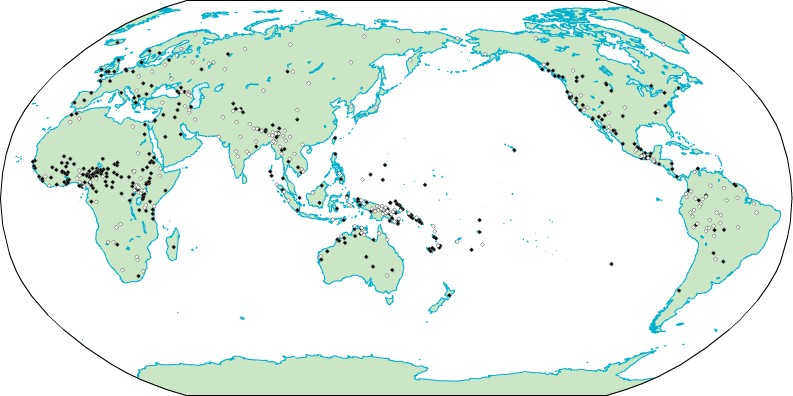
\includegraphics[height=.35\textheight]{figures/10_DistributionDefArticles}
\caption{Distribution of definite articles (black symbols) in a sample of 566 languages \citep{Dryer2005}.}
\label{map:8}
\end{figure}
%\end{styleFigureCaption}
 
%\begin{styleFigureCaption}
\begin{figure}
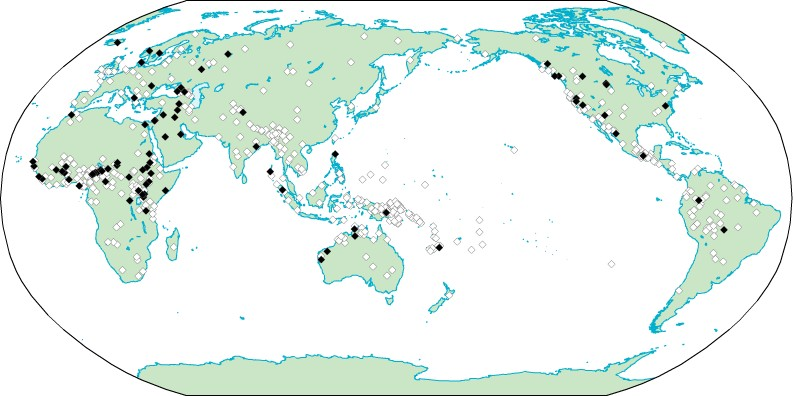
\includegraphics[height=.35\textheight]{figures/11_DistributionDefAffixes}
\caption{Distribution of definite affixes (black symbols) in a sample of 566 languages \citep{Dryer2005}.}
\label{map:8b}
\end{figure}
%\end{styleFigureCaption}

\ea 
	\gl	\label{bkm:Ref93745057}In the street, I saw a cat and a dog. The dog was barking furiously.\footnote{ It is perhaps symptomatic that examples of the anaphoric use of definite noun phrases in the literature tend to contain antecedents which are parts of a conjoined noun phrase: at least in natural speech, pronouns tend to be preferred to full noun phrases as straightforward anaphors in most contexts, and we need a structure such as a conjoined NP for there to be two equally possible antecedents, in which case a definite NP is motivated.}
\z 
\ea 
	\gl	\label{bkm:Ref93745078}I met the author of \textit{Syntactic Structures}.
\z 
\ea 
	\gl \label{bkm:Ref93745091}Please close the door. 
\z 

A highly frequent phenomenon is the “anchoring” of a definite noun phrase to some other element, whether mentioned in the discourse or not (\citet[25]{Fraurud1992}). In \REF{6}, for instance, \textstyleLinguisticExample{the hard disk} is understood as the hard disk of the computer mentioned in the first clause – in other words, the computer serves as the anchor.  This example illustrates what is often called “associative” or “bridging co-reference”\footnote{ Another term that is sometimes used is “bridging anaphora”. Originally, the term “bridging” referred to the “bridging assumption” that provided the link between the definite noun phrase and its anchor. Thus, in (i) we have to make the assumption that the picnic supplies included beer (\citet{ClarkEtAl1974}):\par (i) Mary got some picnic supplies out of the car. The beer was warm. \par But the point that the interpretation of definite noun phrases sometimes involves inferencing gets lost if the term “bridging” is generalized to cases where the assumption in question is trivial or follows from the meaning of the noun phrases involved. In \textit{In this group, the members work well together}, the only assumption necessary to link \textit{the members} to \textit{this group} is that a group has members. } uses of definite noun phrases,

\ea
	\gl	\label{bkm:Ref75942712}I have to fix my computer: there is some problem with the hard disk. 
\z 

In addition to straightforward referential cases as the ones exemplified above, definite articles are also used in generic noun phrases, as in \REF{7}. 

\ea 
	\gl	\label{bkm:Ref123549675}The lion is a mammal.
\z 

In English, this phenomenon is somewhat restricted, but as we shall see below, it plays a more salient role in other languages.

The most common diachronic source for definite articles is demonstrative pronouns, typically distal ones (‘that’). As pointed out by \citet[332]{Lyons1999}, there is a substantial overlap between the domains of use of demonstratives and definite articles, notably in anaphoric function. For instance, in a context like the following, both \textstyleLinguisticExample{that} and \textstyleLinguisticExample{the} are acceptable:

\ea 
	\gl Last year, I saw a film by Ingmar Bergman. I would like to see that/the film again.
\z 

The first stage in the development of definite articles from demonstratives, accordingly, consists in a more general use of a demonstrative in anaphoric function. Such “anaphoric articles” are attested in various languages – \citet[53-54]{Lyons1999} mentions Hausa and Lakota as examples. Geographically closer to the area studied here is spoken Finnish, where at least in some varieties the demonstrative \textstyleLinguisticExample{se }tends to be used in ways suggestive of an “anaphoric article” (see \citet{Laury1997} and, for a more sceptical view, \citet{Juvonen2000}):

\ea\label{}
\langinfo{Finnish}{}{}\\
\gll	...niin  sit  \textbf{se} mies  meni  ja,\\
		so  then  \textbf{this} man  go.{\pst}  and\\
\gll	osti  \textbf{ne} kaikki  ilmapallot\\
		buy.{\pst}  \textbf{this.{\pl}} all  balloon.{\nom}.{\pl}\\
\gll	ja  anto  ne  \textbf{sille} pojalle,\\
		and  give.{\pst}  this.{\pl}  \textbf{this.{\all}} boy.{\all}\\
		
\gll 	ja  sit  \textbf{se} poika...\\
		and then  \textbf{this} boy\\
\glt 	‘…so then the man went and bought all the balloons and gave them to the boy, and the boy…’ (\citet[136]{Juvonen2000})

\z

For an erstwhile demonstrative to look more like the definite articles we are used to from languages such as English, it has to acquire also non-anaphoric uses. Finnish \textstyleLinguisticExample{se }is still unacceptable e.g. in a context as that exemplified in \REF{6}. The mechanism behind an expansion from an anaphoric to a more general definite article is not well understood, but we may note that it involves the elements usually associated with grammaticalization processes: a rise in frequency through the expansion to new contexts where the element becomes obligatory, combined with a loss of prosodic prominence and an ensuing reduction of phonetic weight (what is commonly but misleadingly referred to as “erosion”). 

A language can also have more than one definite article. One way in which such a situation can develop is through separate waves of grammaticalization that give rise to a “layered” system in which two (or more) elements of varying age compete with each other. The youngest element will then typically have the functions that are first to grammaticalize, such as anaphoric ones. This is exemplified by various West Germanic varieties, such as the Fering dialect of North Frisian described by \citet{Ebert1971} (although the actual rules for choosing between the articles are a bit more complicated; for an accessible account see \citet[162]{Lyons1999}). Compare the following examples:

\ea\label{}
\langinfo{North Frisian (Fering dialect)}{}{}\\
\ea 
	\gll 	Hat  kaam  me  \textbf{a} \textbf{maan.}\\
			she  come.{\pst}  with  \textbf{{\deff}} \textbf{man}\\
	\glt 	‘She came with her husband, lit. the man.’
\ex
	\gll	Hat  kaam  me  \textbf{di} \textbf{  maan.}\\
			she  come.{\pst}  with  \textbf{{\deff}} \textbf{man}\\
	\glt	‘She came with the man.’ (\citet[163]{Lyons1999})

	\z 
\z

Among languages whose definite articles would seem to be of a “garden variety” kind, there is in fact considerable variation which is largely attributable to how far the grammaticalization process has gone and which routes it has taken. For example, the English definite article on the whole has a relatively restricted domain of use compared to definite articles in many other languages. Most saliently, as has already been noted, English has a restricted use of definite articles w\textstyleBodytextCChar{i}th generic noun phrases – this will be further discussed in section \sectref{sec:3.2.1}. But English also shows a reluctance to use articles with proper names, in contrast to many other languages, such as Greek and southern German vernaculars, but also many northern Scandinavian vernaculars, to be discussed in section \sectref{sec:3.2.8}. Even in English there are exceptions, such as some types of geographical names, e.g. names of rivers such as \textstyleLinguisticExample{the Thames}. Since proper names are usually seen as “inherently definite”, the use of definite articles would seem to be wholly redundant from the communicative point of view. However, such apparently redundant uses of grammatical elements are typical of later stages of grammaticalization processes and show that the identification of the “function” of a grammatical element is not always easy (\citet[81-86]{Dahl2004}).

The story does not end here, however. A definite article may develop further, expanding its domain of use to a point where it is no longer possible to call it “definite” or even an “article”. This process was described by \citet{Greenberg1978}, who argued that definite articles are the source of various grammatical morphemes.  A particularly notable example of this process involves noun class markers, such  as those found in Bantu languages wherein the affixes are obligatory with nouns irrespective of the context in which they appear. The details of the route to such a situation from “garden variety” definite articles are far from clear. One example of an intermediate stage suggested by Greenberg would be the “specific” articles found in many Oceanic languages which also cover many of the functions of the indefinite article of English, in particular that of introducing new, specific discourse referents. Compare the Samoan article \textstyleLinguisticExample{le} in the following example: 

\ea\label{}
\langinfo{Samoan (Austronesian)}{}{}{}{}\\
\gll	ʽO  \textbf{le} ulug\=aliʽi,  f\=anau  \textbf{l}{}-a  l\=a  tama\\
		{\prs}  \textbf{{\art}} couple  give\_birth  \textbf{{\art}}{}-{\poss}  3{\du}  child\\
\gll	ʽo  \textbf{le} teine  ʽo  Sina.\\
		{\prs}  \textbf{{\art}} girl  {\prs}  Sina\\
\glt ‘There was \textbf{a} couple who had \textbf{a} child, \textbf{a} girl called Sina.’ (\citet[259]{HovdhaugenEtAl1992})

\z

What we find in Scandinavian vernaculars, however, is an expansion of the range of uses of definite articles that goes in a different direction and cannot be described in terms of “specificity” in any sense. The Scandinavian development therefore is of considerable interest for our understanding of the role of definite articles in grammaticalization processes.

\begin{figure}[h]

%\begin{styleBeschriftung}
\includegraphics[height=.5\textheight]{figures/12_Definiteness}
\caption{Definiteness marking of non-modified nouns in Europe west of 30°E (dark grey: free article only, light grey: suffixal marking).}
\label{map:10}
\end{figure}



\subsection{Definite marking in Scandinavian in general}
\label{sec:3.1.4}

As already noted, Western Europe is one of the areas in the world where definite articles are generally present. The distribution is determined by areal rather than by genetic factors. Although definite articles would seem to be a general feature of the Germanic, Celtic and Romance families, this is a late phenomenon not found in the older historical stages of Indo-European. The presence of definite articles in these languages must therefore be attributed to a later spread rather than to inheritance from a parent language. In fact, there is a relatively neat diachronic progression in the appearance of definite articles from the Eastern Mediterranean to north-western Europe, basically in the order of Semitic → Greek → Romance → Germanic, suggesting a rather slow expansion wave which took about two thousand years to complete. The Fenno-Ugric and Slavic languages in Europe are split with respect to definiteness marking, and there is evidence that definite articles are latecomers in these languages also

If we focus on Europe west of 30°E (\figref{map:10}), we find definite articles in one central and two relatively peripheral areas. In the large central area comprising most of Western Europe, definite articles are manifested as free morphemes occurring initially in noun phrases. However, in the two peripheral areas found in Scandinavia and the Balkans, definiteness is marked by suffixing.  This marking occurs in the standard languages of Romanian, Bulgarian, Macedonian, and Albanian. These developments fit less straightforwardly into the general expansion pattern, although the general timing and the closeness to the preposed article area makes areal influence likely here, too. In Scandinavia, the situation is further complicated by the presence of both preposed and suffixed articles, with varying divisions of labour in the individual languages (see \sectref{sec:4.3} for details). It should also be noted here that there are significant differences between the suffixed articles in Scandinavia and those found in the Balkans: the latter should probably be seen as movable clitics rather than suffixes – they typically show up on the first word in the noun phrase, more or less irrespective of its grammatical category (thus, in Macedonian and Bulgarian, definite articles can be cliticized even to possessive pronouns: \textstyleLinguisticExample{moja-ta kniga} ‘my-{\deff} book’). 

The origins of definiteness marking in the Scandinavian languages are rather obscure. Definite articles seem to have been absent from the earliest stages of Old Nordic and there are only sporadic attestations from runic inscriptions. From Sweden, two attestations of what seems to be the same formulaic phrase \textstyleLinguisticExample{kuþ heabi onti-ni }or\textstyleLinguisticExample{ kuþ hialbi *anti-ni} ‘God help soul.{\deff}’ i.e. ‘may God help the soul’ are cited. When written documents start to appear in the 13\textsuperscript{th} and 14\textsuperscript{th} centuries, both preposed and suffixed articles are still rare in many texts, in particular in laws and poetry (which happen to constitute the bulk of the preserved written material); such instances are possibly rarer in Denmark and Sweden than in the West Nordic area. Here are some statistics (\citet[938]{Delsing2002}, based on \citet{Larm1936} and \citet{Skautrup1944}): 

%\begin{styleTableCaption}
\begin{table}
\caption{ Percentage of definite nouns among nouns in general}
\label{tab:1}
\begin{tabular}{ll}
 \lsptoprule
Older Västgöta Law  & 0.5
\\
Uppland Law & 5
\\
Östgöta Law&  7.5
\\
Scanian Law & 8
\\
Jutland Law & 10
\\
\lspbottomrule

\end{tabular}

\end{table}
%\end{styleTableCaption}

The source of the suffixed article is commonly assumed to be an original demonstrative \textstyleLinguisticExample{inn} or \textstyleLinguisticExample{hinn}. The forms with an initial \textstyleLinguisticExample{h-}, which may be due to a reinforcement of \textstyleLinguisticExample{inn} in analogy with other 3\textsuperscript{rd} person pronouns (\citet[135]{Perridon1989}, \citet[723]{Syrett2002}), were only used in preposed position in East Nordic. According to a popular hypothesis (going back to Grimm (1822-40)), the suffixed article originated as an adjectival article in a construction such as \textstyleLinguisticExample{maþr inn gamli }‘man the old’. I think this hypothesis should be viewed with some scepticism. The low frequency in spoken language of the adjectival construction makes it unlikely as a general model for noun phrases (as is also noted by \citet[63]{SaltveitEtAl1971}). There also seems to be little concrete evidence of such a development anywhere. (In the Balkan languages the corresponding constructions would be expressed as ‘man-the old’ and the article would thus not be in the right place relative to the noun.)  Thus, the alternative hypothesis that the suffixed article has developed out of an unstressed postposed demonstrative seems more plausible.  In fact, this phenomenon is exemplified by the inscription \textstyleLinguisticExample{hali hino} ‘[flat] stone \textstyleLinguisticExample{this}’ on the whet-stone of Strøm (Norway) from about 600 C.E. 

With respect to the timetable for the development of the suffixed article, there seem to be two basic views. The first, which assumes that the genesis of the suffixed article in the spoken language is significantly earlier than its appearance in the written language, appears to originate with \citet{Neckel1924}.  This position is also taken in recent works by both \citet[142]{Perridon1989}, who speaks of “a hidden life” of the article “before it starts its public written life”, and \citet[723]{Syrett2002}, who says that “…it seems reasonable to suggest that” the suffixed article “was the end product of an unrelated series of morphological and syntactical developments within the progression from” Ancient Norse to Old Norse (the transitional period between these two being broadly defined as lasting from the 6\textsuperscript{th} century until 1100). 

The main representative of the other view is \citet[938-939]{Delsing2002} who thinks that the suffixed article “developed as an innovation in the 13\textsuperscript{th} century”. (He does not say explicitly what territory this claim is intended to cover, but it is given in the context of a treatment of Old Swedish and Old Danish.) He argues against the view that “the low frequency of articles in the oldest texts can be explained by style”, pointing to the fact that not only legal and poetic texts but also texts which “are written in styles where we would expect an ample use of the articles”,  e.g. the Gutasaga (a text presumed to be from the 13\textsuperscript{th} century and containing a description of the mythical origin of the island of Gotland) and the chronicles from Vidhem [S47], have a low frequency of definite marking. 

Delsing’s discussion of the style question seems to conflate two possible effects of style (or genre) on the use of definite articles: (i) a generally lower frequency of definite marking due to pragmatic reasons; (ii) the possible use of an archaizing language. Thus, he says: “Runic inscriptions, laws and poetry are not the kind of texts where we expect to find articles” (ibid.). There obviously are some text types where definite articles would be infrequent in any language due to a restricted need for definite reference, and runic inscriptions may be cases in point, but this would hardly hold for the other kinds of text mentioned by Delsing. Thus, in a language where definite articles are regularly used, such as English or Modern Swedish, they occur also in laws and poetry. Consider as an example Article 1:1 of the Swedish constitution (\textstyleLinguisticExample{Regeringsformen}), which contains two noun phrases with definite marking:

\ea\label{}
\langinfo{Swedish}{}{}{}{}\\
\gll 	\textbf{Den} \textbf{  offentliga} \textbf{  makten} utövas  under  \textbf{lagarna.}\\
		\textbf{{\deff}} \textbf{public} \textbf{power.{\deff}} exert.{\pass}.{\prs}  under  \textbf{law.{\pl}.{\deff}}\\
\glt  ‘(The) public power is exerted under the laws.’

\z

On the other hand, laws and poetry are genres which are often formulated in an archaizing language and which may thus differ significantly from other text types and in particular from informal spoken language. It may be noted that even contemporary legal Swedish exhibits patterns of article usage which most probably reflect an older stage of development. Thus, until the last decades of the 20\textsuperscript{th} century, it was normal for singular generic noun phrases in legal texts to be used without any article, as in 

\ea\label{}
\langinfo{Swedish}{}{}{}{}\\
\gll	\textbf{Hund} skall  hållas  kopplad  på  \textbf{offentlig} \textbf{  plats.}\\
		\textbf{dog} shall  keep.{\pass}.{\inf}  leash.PP  on  \textbf{public} \textbf{place}\\
\glt ‘A dog shall be kept on a leash in public places (lit: Dog shall be kept leashed on public place)’

\z

The absence of definite articles in medieval legal prose would thus be due to an archaizing language rather than to the general low frequency of definite articles in legal texts. The same goes for poetry, mutatis mutandis. But as Delsing points out, there are other texts which also exhibit a low incidence of definiteness marking. The first text mentioned by Delsing, the Gutasaga, may not be too relevant in this context, since the variety it is written in, Old Gutnish, is not necessarily representative of mainstream Old Swedish.  On the other hand, the Vidhem chronicle (presumed to be written in Västergötland around 1250, although there seems to be no general agreement on this) may be evidence that the use of definite marking was generally restricted in the written language of the period. However, this text is an appendix to the Västergötland law, so one could perhaps expect the style to be close to that of legal language. 

In my opinion, several things speak against the hypothesis that the suffixed article is a 13\textsuperscript{th} century innovation. One is the geographical distribution of the suffixed article: in spite of its low frequency in some early texts, it is attested in the 13\textsuperscript{th} century from all parts of the Scandinavian area: Iceland, Norway, Denmark, and Sweden.  And even earlier, in the first half of the 12\textsuperscript{th} century in Iceland (according to \citet[§1019]{Perridon2002}), there is a consistent use in the First Grammatical Treatise. Moreover, although not frequent, even the very earliest texts in Sweden do contain quite a few definite articles. Thus, the Older Västgöta Law, assumed to be from around 1225, contains 23 instances of suffixed articles (\citet[24]{Larm1936}). This means that, already at this stage, the suffixed article was well enough entrenched to show up in written language all over Scandinavia, although it was still used in a restricted fashion. 

Furthermore, if it were the case that the forms that we see in the oldest texts represent a recent innovation, we would expect them to behave in a way typical of early stages of a grammaticalization process. This is not the case, however. When we first meet the suffixed definite article, it has already reached a relatively advanced stage of grammaticalization. This goes both for form and function: even the earliest attestations are suffixed rather than separate words, and they display non-anaphoric uses (see \sectref{sec:3.1.3}), suggesting a full-fledged definite article. For instance, the earliest attestations from Sweden, \textstyleLinguisticExample{kuþ hialbi antini }‘God help the [i.e. his] soul’ are clear examples of an associative use. The following example from the Vidhem chronicles is also clearly non-anaphoric:

\ea\label{}
\langinfo{Medieval Written Swedish}{}{}{}{}\\
\gll 	Han  læt  gøræ  \textbf{kyrkiunæ} i  agnistaðhum.\\
		he  let.{\pst}  make.{\inf}  \textbf{church.{\deff}.{\acc}} in  Agnestad\\
\glt 	‘He had the church in Agnestad built.’ [S47]

\z

If the rise of definite articles was close in time to the creation of the documents in which they are common, we would expect to find more signs of the early stages of development, both with regard to form and to function.

What was just said about the earliest documented stages is paralleled in the modern forms of Scandinavian: there is no variety that reflects an earlier stage in the grammaticalization process. It should also be noted that the suffixed article has a virtually total coverage in Scandinavian, with the exception of the Jutish dialects in Denmark that use prefixed articles exclusively. Thus, the suffixed articles are also manifested in a remarkably uniform way in the most conservative and peripheral varieties. This is in contrast to the prefixed definite article, which is absent both in modern spoken Icelandic and in the Peripheral Swedish vernaculars, and the indefinite article, which is absent in Icelandic. It is also in contrast to most of the major phonological changes in medieval Scandinavian, which tended to be only partially implemented or not implemented at all in peripheral areas. An example is the monophthongization of the original diphthongs \textstyleLinguisticExample{ai} and \textstyleLinguisticExample{au }to\textstyleLinguisticExample{ e }and\textstyleLinguisticExample{ ö,} respectively,\textstyleLinguisticExample{ }which according to the standard view spread from Denmark to south and central Sweden in the 11\textsuperscript{th} century, but which a millennium later has still not yet been completed in some of the outlying areas, such as northern Norrland, western Dalarna, Österbotten and Gotland.  

\subsection{ Neutralization of the definite-indefinite distinction}
\label{sec:3.1.5}

A fairly common phenomenon, which should be kept apart from the expansion of the definite forms discussed in this chapter, is the partial neutralization of the opposition between definite and indefinite forms: that is, the same form comes to represent both definite and indefinite. For instance, in Orsa (Os), neuter nouns do not distinguish definite and indefinite forms. There is no vernacular in which the neutralization between indefinite and definite is total. Rather, as in Orsa, it tends to hit paradigms only partially. What forms are neutralized varies from place to place, but there are a few typical patterns.

\subsubsection{Neutralization between indefinite and definite in the plural}
 This is probably the most common pattern, being found in relatively many places. 

In Ovansiljan, this appears to be a relatively late development. \citet{Levander1909} describes Elfdalian as still having a distinction for masculine nouns in the nominative plural, e.g. \textstyleLinguisticExample{kaller:kallär }(indefinite and definite nominative plurals of \textstyleLinguisticExample{kall }‘man’), and for some feminine nouns, e.g. \textstyleLinguisticExample{djieter:djietär} (from \textstyleLinguisticExample{djiet} ‘goat’), but not for a feminine noun such as \textstyleLinguisticExample{flugu }‘fly’ which has the only form \textstyleLinguisticExample{flugur} in the nominative plural. However, Levander notes that the distinction is not found in all villages in Älvdalen (with varying isoglosses for different types of nouns), and according to \citet[170]{Levander1928}, it is found in Orsa and Våmhus but not in Mora, Sollerön, Venjan and Ore. In the accusative plural, a distinction between forms such as \textstyleLinguisticExample{kalla:kalla; }exist in all the varieties which retain the nasal vowels, that is, most of Älvdalen, Våmhus and Bonäs (Mora parish). 

In Karleby\footnote{ The previous town of Gamlakarleby and the parish of Karleby were merged into Karleby town in 1977. For simplicity, I use the name “Karleby” throughout. } (NOb), the old indefinite plural forms have disappeared entirely in favour of the definite ones, e.g. \textstyleLinguisticExample{gåǣ7a} ‘(the) yards’, \textstyleLinguisticExample{gatuna} ‘(the) streets’ (\citet[93]{Hagfors1891}). Likewise, in Runö (Es), there is no indefinite-definite distinction at all in the plural (cf. \REF{69} below.)

Neutralization between indefinite and definite in neuter nouns, with zero endings in the nominative/accusative, is found in at least three geographically quite distinct areas: Orsa and northern Venjan in the Ovansiljan area (\citet[133]{Levander1928}) and parts of Värmland. In the Cat Corpus we thus find the following examples of cognates of Swedish \textstyleLinguisticExample{golv} ‘floor’ used as a definite noun with a zero ending:

\ea\label{}
\langinfo{Orsa (Os)}{}{}{}{}\\
\gll	\textbf{Gow} wa  niskajrad.\\
		floor  be.{\pst}  new-clean.PP\\
\glt 	‘The floor was newly cleaned.’ (Cat Corpus)

\z

%\begin{styleTextkrper}
(cf. Swedish \textit{Golvet var nyskurat}) 

%\end{styleTextkrper}

\ea\label{}
\langinfo{Västra Ämtervik (Vm)}{}{}{}{}\\
\gll	Men  nepå  \textbf{gôLv} va  dä  en  hög  mä  matt-traser.\\
		But  down\_on  \textbf{floor} be.{\pst}  it  {\indf}  heap  with  carpet\_rag.{\pl}\\
\glt	‘But on the floor there was a heap of rags.’ (Cat Corpus)

\z

%\begin{styleTextkrper}
(cf. Swedish \textit{Men på golvet var det en hög mattrasor})

%\end{styleTextkrper}

In Orsa and Venjan, where the dative case is still alive, there is also neutralization in the dative of these nouns. 

\subsubsection{Neutralization between indefinite and definite in the dative}
 This appears to be common or even normal in the dative-preserving vernaculars. Thus, according to \citet{Marklund1976}, nouns in \textit{Skelletmål} have two rather than four dative forms – one for singular and one for plural, as in \textstyleLinguisticExample{pigen} ‘the maid’: \textstyleLinguisticExample{pigåm} ‘the maids’ (from \textstyleLinguisticExample{piig} ‘maid’), or just one for both, as in \textstyleLinguisticExample{vaidjåm }‘the wall(s)’. There is thus no definite:indefinite distinction, and although Marklund does not say so explicitly, it appears that the normal interpretation of the dative forms is definite – the ending is also normally added to the definite stem (as in the case of \textstyleLinguisticExample{vaigg}:\textstyleLinguisticExample{vaidjåm}).

The developments are somewhat different in the singular and the plural. In the singular, the indefinite form tends to be marginal or absent, whereas the definite form is stronger; in the plural, it is the definite form that disappears. In Dalecarlian,  the vernacular of Orsa appears to be the only exception in that there are separate forms for definite dative plurals ending in \nobreakdash-\textstyleLinguisticExample{uma, }as in \textit{revuma} ‘fox.{\pl}.{\deff}.{\dat}’. According to \citet{Levander1909}, at the time of his investigation in the first decade of the 20\textsuperscript{th} century, elderly persons in Älvdalen sometimes used definite dative plurals in\textstyleLinguisticExample{ }\textstyleLinguisticExample{\nobreakdash-ume}.  Otherwise, the indefinite dative plural ending \textstyleLinguisticExample{\nobreakdash-um} has been generalized, e.g. Elfdalian \textit{rövum} ‘fox.{\pl}.{\deff}.{\dat}’.

\subsubsection{Neutralization of definiteness in individual lexemes}
Individual lexemes or groups of lexemes sometimes have identical indefinite and definite forms. Thus, in Elfdalian, neuter nouns in \textstyleLinguisticExample{\nobreakdash-ð }have a zero ending in the definite singular nominative and accusative, e.g. \textstyleLinguisticExample{broð} ‘bread’. Many Elfdalian nouns are not inflected at all.  The word for ‘coffee’ is perhaps most notable in this connection; \textstyleLinguisticExample{kaffi}, which like \textstyleLinguisticExample{broð} is highly frequent in contexts in what is below called non-delimited readings, would normally trigger a definite form. 

Neutralization of the definiteness distinction means that the consequences of the changes discussed below are more restricted than they would otherwise be, since in many cases it will not make any difference if an indefinite or a definite form is chosen. It also means that direct comparisons between dialects are not always possible – if you translate an example from one dialect to another, the distinction between definite and indefinite may disappear on the way. 

As I said above and as also argued by \citet{Hummelstedt1934}, neutralization of the definiteness distinction is in principle a different phenomenon from that of extensions of the domain of definite forms. One may of course also speculate whether there is any causal relationship between the processes by which definite forms acquire new uses and the processes by which definite and indefinite forms are neutralized. What could perhaps be expected is that if the definite forms expand too much, the indefinite forms will simply fall into oblivion. This is essentially what seems to happen in the final stages of the grammaticalization paths described by Greenberg. However, confusingly, it is not always the definite forms that win out in the neutralization process: for instance, in Orsa, as we have seen, neuter nouns have zero endings for both indefinite and definite. In other words, the neutralization process may well obliterate the results of the grammaticalization process. On the other hand, given that neutralization is so common, it is somewhat remarkable that speakers are still able to make the distinction when it is needed. Also, there is no consistency in the neutralizations: thus, Orsamål is “radical” in having no definiteness distinction in neuter nouns and “conservative” in being the only vernacular that preserves the same distinction in the dative plural.

It should also be noted that the systems described above often go against general assumptions about markedness relations in morphology (as when a distinction is upheld in oblique cases but not in the nominative) (see Dahl \& Koptjevskaja-\citet{Tamm2006}).

\section{ Survey of extended uses of definites}
\label{sec:3.2}\subsection{ Generic uses}
\label{sec:3.2.1}

Generic noun phrases are used to refer generally to a species (natural kind), class or type of entities.\footnote{ In Swedish grammatical literature, the traditional term used is “allmän betydelse” ‘general meaning’.} There are actually at least two main kinds of generic uses of noun phrases (\citet[19]{KrifkaEtAl1995}). The first, and most well-known, is when the noun phrase occurs in a context in which a general, “law-like” or nomic statement is made about the species, class or type that the noun phrase denotes (\citet{Dahl1973}). The\textbf{ }standard example in the linguistic literature is \textstyleLinguisticExample{Beavers build dams}, in which dam-building is described as a typical activity of beavers. This first type is called “characterizing sentences” by \citet{KrifkaEtAl1995}. In the second type, which they call “kind predications”, the species or kind is referred to without there being a generalization over its members. For instance, in the sentence \textstyleLinguisticExample{The zoologist was studying the beaver}, the beaver species is referred to as the object of the zoologist’s study, but no inference can be drawn about individual beavers.

An interesting typological generalization is that generic uses of noun phrases do not in general have a dedicated mode of expression; rather, several different types of noun phrases may be recruited for those uses. Thus, in English, bare plurals, singulars with indefinite articles, and singulars with definite articles can all be used generically. We may thus also say \textstyleLinguisticExample{A beaver builds dams} and \textstyleLinguisticExample{The beaver builds dams}. There are quite definite restrictions, however. Indefinite singulars can only be used for “characterizing sentences”, not for “kind predications”: \textstyleLinguisticExample{The zoologist was studying a beaver }must mean that he or she was studying a concrete individual (or, possibly, a specific sub-species). Also, in English, definite plurals and definite mass nouns cannot in\textbf{ }general be used generically: \textstyleLinguisticExample{The beavers build dams} must refer to a specific group of beavers and \textstyleLinguisticExample{The gold is expensive} must refer to a specific mass of gold. In this respect, languages with definite articles vary quite considerably. To see this, it is sufficient to compare English to French, where in fact \textstyleLinguisticExample{Les castors construisent des barrages} is the standard way of saying that beavers build dams, and correspondingly, the articleless construction, which is typical of English, is generally ungrammatical. In fact, the French situation appears to be more common among languages with definite articles (at least in Europe). That is, plurals and mass nouns as a rule take a definite article when used generically. \citet{Behrens2005} looked at five European languages – French, English, German, Greek, and Hungarian, and found that French, Greek and Hungarian all behave similarly in this regard, whereas German turned out to be somewhere in the middle. Compare the following example from Behrens’ corpus, \textstyleLinguisticExample{The Little Prince}:

\ea
	\ea {
	\gl English: Flowers are weak creatures.
	}
	\ex {
	\gl German: Die Blumen sind schwach.
	}
	\ex {
	\gl French: Les fleurs sont faibles.
	}
	\ex {
	\gl Greek: Ta lulúdhja íne adhínama.
	}
	\ex {
	\gl Hungarian: A virágok gyengék.
	}
	\z 
\z

%\end{styleExLtrTblii}

%\end{listLFOcvileveli}

Swedish, like German, is an intermediate case in that it sometimes follows the French and sometimes the English pattern. Thus, Swedish uses a definite NP in \textstyleLinguisticExample{Livet är kort} ‘Life is short’ (cf. French \textstyleLinguisticExample{La vie est brève}) but like English prefers a bare noun in \textstyleLinguisticExample{Guld är dyrt} ‘Gold is expensive’. Possibly, Swedish is slightly more restrictive than German in the use of definite generics: it would seem more natural to use an indefinite plural in the translation of \REF{17} than a definite one:

\ea\label{}
\langinfo{Swedish}{}{}{}{}\\
\gll	\textbf{Blommor} är  veka  varelser.\\
		\textbf{flower.{\pl}} be.{\prs}  weak.{\wk}  being.{\pl}\\
\glt	‘Flowers are weak beings.’

\z

However, many Peripheral Swedish varieties behave more like French in this respect, with an across-the-board use of definite forms in generics. We thus find examples such as the following:

\ea\label{}
\langinfo{Älvdalen (Os)}{}{}{}{}\\
\gll	\textbf{Guld} \textbf{ið} ir  dyrt.  \\
		\textbf{gold.{\deff}} be.{\prs}.{\sg}  expensive.{\n}  \\
\glt	‘\textbf{Gold} is expensive.’ (questionnaire)

\z

Generic uses of definites seem to be among the most widespread of the extended uses of definites found in the Peripheral Swedish area. They are thus characteristic not only of Upper Norrland and Upper Dalecarlian but also of regions such as Värmland, southern Finland, and Norway. Compare the following examples:

\ea\label{}
\langinfo{Östmark (Vm)}{}{}\\
\gll	\textbf{Kaffen} \textbf{ä} \textbf{  allt} \textbf{  bätter} \textbf{  än} \textbf{ten.}\\
		\bfseries coffee.{\deff}  be.{\prs}  sure  better   than  tea.{\deff}\\
\glt	‘Coffee is sure better than tea.’ (\citet{Broberg1936})

\z

\ea\label{}
\langinfo{Pernå (Ny)}{}{}\\
\gll	\textbf{Björc(in,} han  ä  nɷ  bäter  ti  m\={ö}bler,\\
		\textbf{birch.{\deff}} it  be.{\prs}  surely  better  for  furniture.{\pl}\\
\gll 	men  han  ä  so  h\=order  ti  arbita.\\
		But  it  is  so  hard  {{\inf}m}   work.{\inf}\\
\glt	‘Birch, it is better for furniture, but it is so hard-worked.’ (Lundström (1939: 13-14))

\z

\ea\label{}
\langinfo{Ingå (Ny)}{}{}\\
\gll	Va  hadde  man  för  tjö:rdo:n  ti  de:?  {}-  \textbf{Tjärran.}\\
		what  have.{\pst}  one  for  vehicle  for  that    \textbf{cart.{\deff}}\\
\glt	‘What kind of vehicle did they use for that? – A [lit. the] cart.’ (\citet[42]{Harling-KranckEtAL1998})

\z

\ea\label{}
\langinfo{Tromsø (Troms, Norway)}\label{bkm:Ref135628619}{}{}\\
	\ea
		\gll	Det  e  mer  varme  i  \textbf{kola} enn  i  \textbf{veden.}\\
				It  be.{\prs}  more  heat  in  \textbf{coal.{\deff}} than  in  \textbf{firewood.{\deff}}\\
		\glt	‘There is more heat in coal than in firewood.’ (\citet[19]{Iversen1918})

	\ex
		\gll	\textbf{Ulvan} e’  minder  som  \textbf{bjørnan.}\\
				\textbf{Wolf.{\deff}.{\pl}} be.{\prs}  small.{\cmpr}  than  \textbf{bear.{\deff}.{\pl}}\\
				
		\glt	‘Wolves are smaller than bears.’ (\citet[18]{Iversen1918})
	\z 
\z

The examples in \REF{23} are the only ones that I have found in the literature from Norway, but reactions from Norwegian linguists suggest that such generic uses are in fact more widespread. 

As noted above, Delsing’s “tentative” map of the “partitive” uses of definites in Scandinavia shows all of Northern Sweden (and a strip in Norway along the Swedish border in Trøndelag) as having “partitive articles where the standard language has generic naked forms”, the southern border coinciding more or less with the \textstyleLinguisticExample{limes norrlandicus.} More specifically, it passes through northern Värmland and southern Dalarna and cuts Gästrikland in two. As for Värmland, Delsing’s line is roughly at the height of Torsby and Ekshärad, but the Cat Corpus examples – from Västra Ämtervik (Fryksdalen) and Mangskog – give evidence that the border goes at least 40-50 kilometers further south in Värmland: 

\ea
	\ea { \label{}
	\langinfo{Västra Ämtervik (Vm)}{}{}\\
	\gll	\bfseries FôggLân  skâ  en  fôll  int  mat…\\
			\bfseries bird.{\pl}.{\deff}  shall.{\prs}  one  {\prag}  {\neg}  feed\\
	}
	\ex {
	\langinfo{Mangskog (Vm) }{}{}\\
	\gll	\bfseries Fugglane  skâ  en  föll  inte  mate…\\
			\bfseries bird.{\pl}.{\deff}  shall.{\prs}  one  {\prag}  {\neg}  feed\\
	\glt 	‘Birds, you should not feed…’ (Cat Corpus)
	}
	\z 
\z

%\begin{styleTextkrper}
The use is not consistent, however – in the following example the indefinite form is used:

%\end{styleTextkrper}

\ea\label{}
\langinfo{Västra Ämtervik (Vm)}{}{}\\
\gll 	\textbf{Sockerkak} ä  dä  bäst  Kâtt’n  vet.\\
		\textbf{Sponge\_cake} be.{\prs}  {\deff}.{\n}  best  cat.{\deff}  know.{\prs}\\
\glt ‘Sponge cake is Cat’s favourite.’ (Cat Corpus)

\z

\ea\label{}
\langinfo{Mangskog (Vm)}{}{}\\
\gll 	\textbf{Sockerkake} ä  dä  bäste  Katten  vet.\\
		\textbf{Sponge\_cake} be.{\prs}  {\deff}.{\n}  best  cat.{\deff}  know.{\prs}\\
\glt 	‘Sponge cake is Cat’s favourite.’ (Cat Corpus)

\z

On the other hand, there is rather little evidence for generic uses of noun phrases in the rest of Delsing’s southern area. Delsing does not himself provide any such examples, and the Cat Corpus evidence is rather negative, in the following sense: In the translations of \REF{24}{}-\REF{25}, no definite forms show up in texts from Hälsingland (3 texts), Härjedalen (1 text), and Dalarna outside the Ovansiljan area (about ten texts). (The examples from Ovansiljan are sometimes ambiguous due to the neutralization of the definiteness distinction in the plural.) Consider, for example, the following three translations from Hälsingland:\footnote{ The endings in the plural tend to be confusing – for instance, the -a ending is definite in some vernaculars and indefinite in others. In the case of Färila and Järvsö the indefinite plural of ‘bird’ is \textit{fôggla} and the definite plural is \textit{fôgglan}. }

\ea
	\ea{
	\langinfo{Färila (Hä)}{}{}\\
	\gll	\textbf{Fôggǣ7â} skâ  mânn  fäll  int  matâ,  häll!\\
			\textbf{Bird.{\pl}} shall.{\prs}  one  {\prag}  {\neg}  feed.{\inf}  either\\
	}
	\ex {
	\langinfo{Forsa (Hä)}{}{}\\
	\gll	\textbf{Fug}l\textbf{ar} ska  man  fell  int  mata  e.\\
			\textbf{bird.{\pl}} shall.{\prs}  one  {\prag}  {\neg}  feed.{\inf}  {\neg}\footnotemark{}\\
	}
	
	\ex{
	\langinfo{Järvsö (Hä)}{}{}\\
	\gll	\textbf{Fôggla} ska  man  fell  int  mata,  e.\\
			\textbf{bird.{\pl}} shall.{\prs}  one  {\prag}  {\neg}  feed.{\inf}  {\neg}\\
	\glt ‘Birds, you should not feed…’ (Cat Corpus)
	}
	\z 
\z

\footnotetext{ The morpheme \textit{e} is a reinforcing element that co-occurs with negation often enough to warrant talking of a double negation construction. It is common in vernacular texts from Uppland and Hälsingland.}

%\begin{styleTextkrper}
Likewise Västerdalarna:

%\end{styleTextkrper}

\ea
	\langinfo{Transtrand (Vd)}{}{}\\
	\ea {
		\gll	\textbf{Göll} e  dirt.\\
				\textbf{gold} be.{\prs}  expensive\\
		\glt 	‘Gold is expensive.’ (questionnaire)
	}
	\ex {
		\gll 	\textbf{Häster} kut  fort.\\
				\textbf{horse.{\pl}} run.{\prs}  fast\\
		\glt 	‘Horses run fast.’ (questionnaire)
	}
	\z 
\z

\subsubsection{Citation uses}
 Among uses of definite nouns that are close to generics, one can mention meta-linguistic uses or what is commonly called “citation forms”. This kind of use seems to be quite common in many parts of the peripheral area. Thus, speakers who are asked to write down word lists often quote nouns in the definite form. This use of definite forms is already reflected in the word lists of \textit{Pitemål} compiled by the philologist Johan Ihre in the 18\textsuperscript{th} century (\citet{Reinhammar2002}). 

Some clear examples of citation uses are:

\ea \label{} 
\langinfo{Ersmark (NVb) }{}{}\\
\gll 	He  kall  ve  fö  \textbf{sjanostn} för  gammalt.\\
		it  call.{\prs}  we  for  \textbf{sand\_cheese.{\deff}} for  old.{\n}\\
\glt 	‘This we call “sand cheese” of old.’ [S43]

\z

\ea \label{} 
\langinfo{Svartlå, Överluleå (Ll)}{}{}\\
\gll Jö  tråo  dom  kåles  \textbf{skråkaran.}\\
I  think.{\prs}  they  call.{\pass}.{\prs}  \textbf{“skråkar”.{\deff}.{\pl}}\\
\glt ‘I think they are called “skråkaran” ‘ [S45]

\z

Definite forms in citation uses are occasionally mentioned in the literature. Thus, \citet[282]{ÅgrenEtAl1954} say that if you ask a Norrlandic farmer what the berries that grow along the sides of the field are called, he answers \textstyleLinguisticExample{Åkerbära} ‘the polar cloudberries’. According to \citet[82]{Lagman1979}, the definite form shows up “to a certain extent” as the “lexical form” in Estonian Swedish. Thus, he says, the answer to the question “What is ‘white horse’ in Nuckö Swedish?” would be \textstyleLinguisticExample{hoit aiken} ‘white horse.{\deff}’. \citet[8]{Steensland1994}, in his book on Elfdalian plant names, says that he uses indefinite forms throughout, “although this can often appear unnatural to an Elfdalian”.  “In Elfdalian definite forms are most often used when a plant is named.”\footnote{ “Jag återger i regel de älvdalska växtnamnen i obestämd form, trots att detta många gånger kan te sig onaturligt för en älvdaling. I älvdalskan använder man nämligen oftast bestämd form, då man benämner en växt.¨’}

\subsection{Non-delimited uses}
\label{sec:3.2.2}

A major type of extended uses of definite forms in the Peripheral Swedish area are the ones I shall call \textbf{non-delimited}. Consider the following sentence from the Cat Corpus: 

\ea 
	\ea {
	\langinfo{Swedish}{}{}\\
	\gll 	Ja,  bara  jag  har  fått  in  vedbördan,\\
			yes  only  I  have.{\prs}  get.{\supp}  in  wood\_bundle.{\deff}\\
	\gll 	så  ska  jag  värma  \textbf{mjölk} åt  honom.\\
			so  shall.{\prs}  I  warm.{\inf}  \textbf{milk} for  him\\
	}
	\ex {
	\langinfo{Skellefteå (NVb)} \label{bkm:Ref110672187}{}{}\\
	\gll 	Jå,  bara  I  ha  börä  ein  veabåla,\\
			yes  only  I  have.{\prs}  get.{\supp}  in  wood\_bundle.{\deff}\\
	\gll 	sä  skå  I  väärm  \textbf{mjölka} åt  ‘n.\\
			so  shall.{\prs}  I  warm.{\inf}  \textbf{milk.{\deff}} for  him\\
	}
	\ex {
	\langinfo{Orsa (Os)}{}{}\\
	\gll 	Ja,  bara  i  a  fendji  in  widn\\
			yes  only  I  have.{\prs}  get.{\supp}  in  firewood.{\deff}\\
	\gll 	sö  skari  wärm  \textbf{mjötje} a  num.\\
			so  shall.{\prs}\_I  warm.{\inf}  \textbf{milk.{\deff}} for  him\\
	\glt 	‘As soon as I have got the wood bundle into the house, I’ll warm some milk for him.’ (Cat Corpus)
	}
	\z 
\z

Here, both \textit{Skelletmål} and the Orsa vernacular use the definite form of the noun \textstyleLinguisticExample{milk} in the second clause, although an indefinite form would be expected from the point of view of Standard Swedish, since there is no earlier mention of milk in the text. 

Such uses have often been called “partitive” in the literature, which seems natural in view of the fact that they by and large correspond to the use of the the “partitive articles” in French and Italian, and also are generally translatable by the partitive case in languages such as Finnish and Estonian. As pointed out in \citet[525]{Koptjevskaja-Tamm2001}, however, the term “partitive” is better reserved for constructions which express part-whole relationships in a narrower sense, such as \textstyleLinguisticExample{a piece of the cake}. For constructions that derive historically from partitive constructions but are synchronically used to express a non-specified quantity of something, such as noun phrases with partitive articles in Romance languages, Koptjevskaja-Tamm uses the term “pseudo-partitive”. This term, however, is less suitable for patterns that have no direct link to partitive constructions in the proper sense, and I therefore prefer the term “non-delimited” here. “Non-delimited” means that the noun phrase contains no indication of a quantity such as \textstyleLinguisticExample{a cup of} in \textstyleLinguisticExample{a cup of tea }or \textstyleLinguisticExample{much} in \textstyleLinguisticExample{much beer}. The lexical heads of non-delimited NPs are either mass nouns or plural count nouns. In English and Central Scandinavian, they would typically be “bare NPs”, e.g. beer in I am drinking beer. 

\citet[51]{Delsing1993} notes that the non-delimited uses of definite forms, or as he calls them, noun phrases with “partitive articles”, can be used in existential constructions with a dummy subject, as in the following examples: 

\ea\label{}
\langinfo{“North Swedish” (location unspecified)}{}{}\\
\gll 	Hä  finns  \textbf{vattne} däri  hinken.\\
		it  exist.{\prs}  \textbf{water.{\deff}} there\_in  bucket.{\deff}\\
\glt 	‘There is water in the bucket.’

\z

\ea
\gll 	Hä  väks  \textbf{granän} överallt.\\
		it  grow.{\deff}  \textbf{fir.{\deff}.} everywhere\\
\glt 	‘Fir trees grow all around.’
\z

From this observation, Delsing draws the conclusion that these forms are not really definite, and that we are not dealing with “definite forms” or a “definite article” but rather with manifestations of a “partitive article” separate from the ordinary definite article or definite forms. He also includes generic uses of definite forms under this heading. 

The definiteness constraint on NPs in the Swedish dummy subject construction (which is similar to the English one) makes it possible to use this construction as a test on definiteness in Swedish. The definiteness constraint is not universal, however; it does not hold for the corresponding constructions in German:

\ea \label{} 
\langinfo{German}{}{}\\
\gll Es  kommt  \textbf{der} \textbf{  Zug} von  Kiel.\\
it  come.{\prs}  \textbf{{\deff}.{\m}.{\nom}} \textbf{train} from  Kiel\\
\glt ‘The train from Kiel comes/is coming.’

\z

It follows that the definiteness constraint is not necessarily applicable to the varieties discussed here. Furthermore, it is not obvious that there is a unified notion of definiteness that can be applied at all levels of description. What is marked by a definite article may well be semantically or pragmatically indefinite, and vice versa. The postulation of two separate entities underlying the various uses of definite forms detracts attention from the fact that these forms are diachronically connected and may also be argued to form a continuum synchronically. We may of course decide that the distribution of definite forms in Peripheral Swedish vernaculars is too different from that of the entities we usually call definite articles to deserve that name. I think practical considerations speak in favour of not inventing a new term here. Delsing’s proposal, “partitive article”, could of course only cover the extended uses of definite forms. However, Delsing applies it not only to non-delimited uses but also to generic ones. Since there are dialects which have generic but no non-delimited uses of definites, this has the rather peculiar consequence that there would be partitive articles whose only reading is generic. Generic readings are not found with partitive articles in Romance. Instead, those languages as a rule mark generic noun phrases by definite articles. Similarly, with respect to case-marking in Fenno-Ugric, generic NPs pattern with NPs that have definite reference. Furthermore, even in Swedish, the definite form is used with generic noun phrases in various contexts (above all with singular nouns), which, on Delsing’s proposal, would make the borderline between the definite and the partitive articles look a bit arbitrary. There is good reason, as we shall see, to assume that generic readings of definites are diachronically prior to non-delimited ones. We shall also see that there are various other extended uses of definites for which “partitive” is not a natural label. In view of this, I find the term “partitive article” rather inadequate for the extended uses of definites in Peripheral Swedish. (\citet{BergholmEtAl1999} take this line of reasoning even further, labelling all extended uses of definite forms “generic”.)

As examples of extended uses of definite articles in the literature, one often finds expressions such as ‘pick berries’. In sentences such as \REF{33} and \REF{34} it is natural to use a non-delimited noun phrase since it does not really make sense to specify a quantity. 

\ea
\gl \label{bkm:Ref78699401}I am picking berries.  
 \z

 \ea 
 \gl \label{bkm:Ref95014405}I pick berries in summer.
 \z 

There are, however, other contexts where a quantity is at least implied:

\ea
\gl \label{bkm:Ref78699451}I picked berries today. 
\z 

In contradistinction to \REF{33}, where the activity is still going on and the result is yet undetermined, \REF{35} implies the existence of a specific quantity of berries that I have picked. In similar contexts, English bare nouns are in competition with nouns preceded by quantifiers, such as with the unstressed variant of \textstyleLinguisticExample{some} sometimes denoted in the linguistic literature as \textstyleLinguisticExample{sm}):

\ea
\gl I picked some berries today.  
\z

%\end{listLFOileveli}

There may be some variation among languages as to the choice between constructions with and without quantifiers. It does appear that, in many Peripheral Swedish vernaculars, cognates of Swedish \textstyleLinguisticExample{någon} ‘some’\textstyleLinguisticExample{ }have undergone a development which has led to a considerably wider use than in the standard language. They thus show up both when Swedish has quantifiers such as \textstyleLinguisticExample{lite} ‘a little’ and when it uses bare noun phrases. \citet[110]{Levander1909} notes that Elfdalian \textstyleLinguisticExample{någär }is used in “indefinite individualization” in a way that differs from what is found in Swedish, as in 

\ea \label{} 
\langinfo{Åsen, Älvdalen (Os)}{}{}\\
\gll Ig  al  etter  \textbf{nog} \textbf{  broðe.}\\
I  shall.{\prs}  after  \textbf{some} \textbf{bread.{\dat}}\\
\glt ‘I’ll go and get some bread.’ 

\z

Similarly, compare \REF{30}(b) in \textit{Skelletmål}, where a definite form \textstyleLinguisticExample{mjölka} is used, with the corresponding sentence in Ume-Sävarmål, from the southern part of the same province (Västerbotten):

\ea \label{} 
\langinfo{Sävar (SVb)}{}{}\\
\gll Joo,  barra  ja  ha  byre  in  veabÖLa,  \\
yes  only  I  have.{\prs}  get.{\supp}  in  wood\_bundle.{\deff}  \\
\gll sä  ska  ja  väärm  \textbf{na} \textbf{mjÖLk} ått  ‘n.\\
so  shall.{\prs}  I  warm.{\inf}  \textbf{some} \textbf{milk} for   him\\
\glt ‘As soon as I have got the wood bundle into the house, I’ll warm (some) milk for him.’ (Cat Corpus)

\z

The \textit{Skelletmål} translator has here chosen to use a definite noun \textstyleLinguisticExample{mjölka, }whereas the Sävar translation contains \textstyleLinguisticExample{na }followed by an indefinite form of the noun \textstyleLinguisticExample{mjÖlk}. However, \textit{Skelletmål} as described by \citet{Marklund1976} is not alien to an extended use of \textstyleLinguisticExample{na}. \citet[43]{Marklund1976} says that \textstyleLinguisticExample{na} is used often enough to “lose its character as a pronoun in the proper sense and may even sometimes lack a standard language counterpart”, especially “with adjectives in negated and interrogative clauses”, which sounds like a straightforward description of a grammaticalized item. Some examples are:

\ea \label{} 
\langinfo{\textit{Skelletmål (}NVb)}{}{}\\
\gll Hæ  e  kåmme  \textbf{na} \textbf{  mââng?}\\
have.{\prs}  it  come.{\supp}  \textbf{some} \textbf{many}\\
\glt ‘Have many [people] arrived?’ (\citet[43]{Marklund1976})

\z

\ea \label{} 
\langinfo{\textit{Skelletmål} (NVb)}{}{}\\
\gll Eint  vær  I  dâ  \textbf{na} \textbf{rädd.}\\
{\neg}  be.{\pst}  I  then  \textbf{any} \textbf{afraid}\\
\glt ‘I wasn’t afraid then at all.’ (\citet[43]{Marklund1976})

\z

For \textit{Pitemål}, \citet[19]{Brännström1993} says: “In Pitemål, \textit{na} is used as an indefinite article in the plural”, quoting examples such as the following:

\ea\label{}
\langinfo{\textit{Pitemål }(Pm)}{}{}\\
\gll Hä  kom  \textbf{na} \textbf{  fLi{\textasciigrave}ttjom} ötät  väjen.\\
it  come.{\pst}  \textbf{some} \textbf{girl.{\dat}.{\pl}} along  road.{\deff}\\
\glt ‘There came some girls along the road.’ (\citet[19]{Brännström1993})

\z

\ea
\gll Dji´v  mä  \textbf{na} \textbf{  kòrvom!}\\
give.{\imp}  PRO.1{\sg}.{\obl}  \textbf{some} \textbf{sausage.{\dat}.{\pl}}\\
\glt ‘Give me some sausages!’ (\citet[19]{Brännström1993})

\z

(For a discussion of the case marking, see \sectref{sec:3.2.4} below.) 

In other words, \textstyleLinguisticExample{na}{}-marked noun phrases have encroached on the territory of non-delimited definites in part of the Peripheral Swedish area. 

\begin{figure}[h]
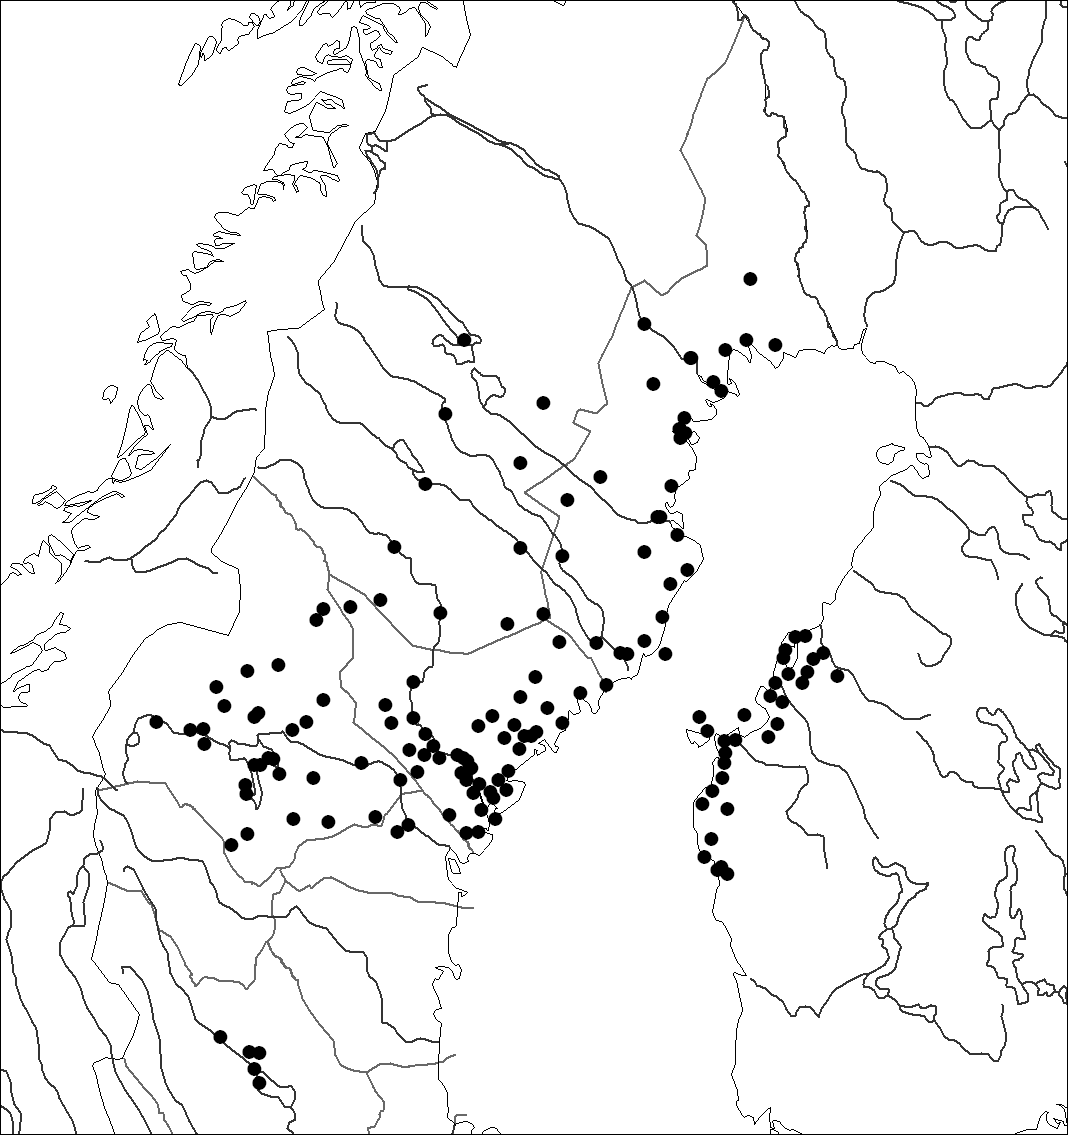
\includegraphics[height=.5\textheight]{figures/13_PresentDayDistribution}
\caption{Present-day distribution of non-delimited uses of definite nouns.}
\label{map:11}

\end{figure}

\subsection{ Areal distribution of non-delimited uses}

Although the map in \citet{Delsing2003a} shows non-delimited uses of definite nouns as being restricted to the Swedish-speaking areas of Norrbotten, Västerbotten, Österbotten, Ångermanland and parts of Jämtland, the distribution is in fact wider. In addition to the northern area just mentioned, non-delimited definites are quite strongly represented in the Ovansiljan area, and more or less sporadic examples are found also elsewhere in the Peripheral Swedish area. We shall first look at the two core areas.

\subsubsection{The northern core area}
It appears that non-delimited definites are normal in all Westrobothnian, Norrbothnian, Angermannian, and Ostrobothnian vernaculars, and the usage is fairly stable. It is striking that non-delimited definites are even found in the so-called “settler dialects” (\textstyleLinguisticExample{nybyggarmål}) of the province of Lappland, which are usually said to be strongly influenced by Standard Swedish. Compare the following example from Arvidsjaur in the south-western Lappland:

\ea \label{} 
\langinfo{Arvidsjaur (Nm)}{}{}\\
\gll Jaa,  I  ska  berätt  för  je\\
yes  I  shall.{\prs}  tell.{\inf}  for  you\\
\gll då  ji  å  a  Karolina  nåppe  \textbf{snottren} i  höst.\\
when  I  and  {\pda}.{\f}  Karolina  pick.{\pst}  \textbf{cloudberries.{\deff}.{\pl}} in  autumn\\
\glt ‘Well, I’ll tell you how Karolina and I picked cloudberries last autumn.’\textsuperscript{ }[S4]

\z

In my opinion, Jämtland should also be included in the northern core area. Delsing is a bit vague here: he first mentions examples of definite forms after quantifiers from the Indal river valley, and then says that “partitive articles” (apparently in general) are “more frequent there than around Lake Storsjön and westward” (\citet[19]{Delsing2003a}). On the map, he draws the western border of the use of the partitive article in non-delimited uses at the parish of Lit – this seems to be based on the distribution of quantified uses. However, it is fairly clear that non-delimited uses can be found all over the province (Bo Oscarsson, personal communication). The following is an example from the parish of Kall in the western part of Jämtland (the informant was born around 1850, the text was written down in 1908):

\ea \label{} 
\langinfo{Kall (Jm)}{}{}\\
\gll En  vakker  ‘n  dag  rest  ‘n  åt  skoga\\
one  beautiful  {\pia}  day  go.{\pst}  he  to  forest.{\deff}\\
\gll å  skull  skaff  \textbf{ven.}\\
and  will.{\pst}  get.{\inf}  \textbf{wood.{\deff}}\\
\glt ‘One day he went to the forest to get firewood.’ [S11]

\z

\textbf{The southern core area (Ovansiljan)}. This area is much smaller than the northern one, and the strength of non-delimited uses is also more variable, suggesting a general receding tendency. The most stable usage is found in the more conservative vernaculars of Älvdalen, Våmhus, and Orsa. \citet[95]{Levander1909} quotes the following examples:

\ea\label{}
\langinfo{Älvdalen (Os)}{}{}\\
\gll Ulum  fǫ  \textbf{stjyreð} et  middags.  \\
shall.{\prs}.1{\pl}  have.{\inf}  \textbf{curdled\_milk.{\deff}} to  dinner.{\gen}\footnotemark{} \\
\glt ‘We’ll have curdled milk for dinner.’

\z
\footnotetext{ This is a fossilized “old” genitive, see \sectref{sec:5.4.2}.} 
\ea
\gll Will  du  fǫ  \textbf{snuseð} min  mig?\\
want.{\prs}  you  have.{\inf}  \textbf{snuff.{\deff}} with  PRO.1{\sg}.{\obl}\\
\glt  ‘Do you want to have snuff from me?’

\z

More recent attestations can be quoted from Bengt Åkerberg’s translation of the novel \textstyleLinguisticExample{Hunden} by Kerstin Ekman:

\ea\label{}
\langinfo{\label{bkm:Ref113183734}Älvdalen (Os) }{}{}\\
	\ea { 
		\gll 	Eð  liep  nið  \textbf{smeltwattneð} i  uäl\k{u}.  \\
				it  run.{\pst}  down  \textbf{melting\_water.{\deff}} in  hole.{\deff}.{\acc}  \\
		\glt 	‘Melting water was running down into the hole.’ [S9]
	}
	\ex {
	\gll 	Måyre;  war  ikåv  min  \textbf{wattne;.}\\
			marsh.{\deff}  be.{\pst}  pregnant  with  \textbf{water.{\deff}.{\dat}}\\
	\glt 	‘The marsh was pregnant with water.’ [S9]
	}
	\z
\z 
	
	(a) demonstrates the possibility of using a definite form in the dummy subject construction, showing that this is indeed possible also in the Ovansiljan area. 

Also in Mora, which has always been the centre of the Ovansiljan region, non-delimited uses of definite forms are relatively strong. Thus, the translation of \REF{30} in the Mormål version in the Cat Corpus is:

\ea \label{} 
\langinfo{Mora (Os)}{}{}\\
\gll Ja,  bar  I  a  feir-in  wiråbördu,\\
yes  only  I  have.{\prs}  get\_in.{\supp}  wood\_bundle.{\deff}\\
\gll så  ska  I  werm  \textbf{mjotse} a  onum.\\
so  shall.{\prs}  I  warm.{\inf}  \textbf{milk.{\deff}} for  PRO.3{\sg}.{\m}.{\dat}\\
\glt ‘As soon as I have got the wood bundle into the house, I’ll warm some milk for him.’ (Cat Corpus)

\z

An example from the Bible texts in [S20]\textstyleLinguisticExample{:}

\ea \label{} 
\langinfo{\label{bkm:Ref123968060}\textit{Östnors-seljamål} (Os)}{}{}\\
\gll Finns  ä  nån  …  såm  djäv  dem\\
exist.{\prs}  it  somebody    that  give.{\prs}  3{\pl}.{\obl}\\
\gll jen  wårm  när  dem  fråg  ettär  \textbf{fistjen?}\\
{\indf}  snake  when  they  ask.{\prs}  after  \textbf{fish.{\deff}}\\
\glt ‘Is there anybody … who gives them a snake when they ask for fish?’ (Matt. 7:10) [S20]

\z

In an older text we find the following:

\ea \label{} 
\langinfo{\label{bkm:Ref123968062}Mora (Os)}{}{}\\
\gll Ä  wa  je  keLing  frammä,  so  add  selt  \textbf{brendunä.}\\
there  be.{\pst}  {\indf}  woman  out\_there  {\rel}  have.{\pst}  sell.{\supp}  \textbf{aquavit.{\deff}}\\
\glt ‘There was a woman out there, who had sold aquavit.’ [S46]

\z

(It may be noted that both \REF{47} and \REF{48} contain dummy subjects.)

However, the use of definite forms may be receding in Mormål. Compare the following parallel examples from the Elfdalian translation of the Gospel of John (\textstyleLinguisticExample{Juanneswaundsjila;}) and \textstyleLinguisticExample{Mormålsbibeln}:

\ea 
	\ea{ \label{}
	\langinfo{Älvdalen (Os)}{}{}\\
	\gll 	Ed  so  ar  kumid  til  åv  tjyöt\k{i},  ed  ir  \textbf{tjyöted…}\\
			it  {\rel}  have.{\prs}  come.{\supp}  to  of  flesh.{\deff}.{\dat}  it  be.{\prs}  \textbf{flesh.{\deff}}\\
	\glt 	‘That which is born of flesh is flesh...’ (John 3:6) [S37]
	}
	\ex {
	\langinfo{\emph{Önamål} (Mora, Os)}{}{}\\
	\gll 	Er  så  a  kem-ti\textbf{l} åv  \textbf{tjöt} \textbf{  e} \textbf{  tjöt…}\\
			it  {\rel}  have.{\prs}  come\_about.{\supp}  of  \textbf{flesh} be.{\prs}  \textbf{flesh}\\
			
	\glt ‘That which is born of flesh is flesh...’\textbf{ }[S20]\textbf{ }
	}
	\ex {
	\langinfo{Älvdalen (Os)}{}{}\\
	\gll 	…ig  ar  kumid  og  döper  min  \textbf{wattne;.}\\
			I  have.{\prs}  come.{\supp}  and  baptize.{\prs}  with  \textbf{water.{\deff}.{\dat}}\\
	\glt 	‘…I have come to baptize with water.’ [S37]
	}
	\ex {
	\langinfo{\textit{Önamål} (Mora, Os)}{}{}\\
	\gll	…ar  I  kem  å  döpär  min  \textbf{wattn.}\\
			have.{\prs}  I  come.{\supp}  and  baptize.{\prs}  with  \textbf{water}\\
			
	\glt	‘…I have come to baptize with water.’ [S20]
	}
	\z 
\z

Among the other parishes in Ovansiljan, non-delimited definites are used fairly systematically in the Cat Corpus texts from Orsa and Våmhus: 

\ea 
	\ea {
	\langinfo{Orsa (Os)}{}{}\\
	\gll 	Ja,  bara  i  a  fendji  in  widn\\
			yes  only  I  have.{\prs}  get.{\supp}  in  firewood.{\deff}\\
	\gll 	så  skari  wärm  \textbf{mjötje} a  num.\\
			so  shall.{\prs}\_I  warm.{\inf}  \textbf{milk.{\deff}} for  PRO.3{\sg}.{\m}.{\dat}\\
	}
	\ex {
	\langinfo{Våmhus (Os)}{}{}\\
	\gll 	Ja,  bara  i  a  faið  in  wi:ðn,  \\
			yes  only  I  have.{\prs}  get.{\supp}  in  firewood.{\deff}  \\
	\gll 	so  ska  i  werm  \textbf{miö:ts\={i}} a  na.\\
			so  shall.{\prs}  I  warm.{\inf}  \textbf{milk.{\deff}} for  PRO.3{\sg}.{\f}.{\dat}\\
	\glt  	‘As soon as I have got the wood bundle into the house, I’ll warm some milk for him.’ (Cat Corpus)
	}
	\z 
\z

Similarly, in the extensive questionnaire materials from Orsa collected by Eva Olander, the overwhelming majority of the informants used definite forms in examples such as the following:

\ea \label{} 
\langinfo{Orsa (Os)}{}{}\\
\gll An  drick  \textbf{mjötji.}\\
he  drink.{\prs}  \textbf{milk.{\deff}}\\
\glt ‘He drinks milk.’

\z

In Sollerön, the use of non-delimited definites appears to be weaker. Thus, according to informants, it would be most natural to use an indefinite form in the following example:

\ea \label{} 
\langinfo{Sollerön (Os) }{}{}\\
\gll An  drikk  \textbf{mjok.}\\
he  drink.{\prs}  \textbf{milk}\\
\glt ‘He is drinking milk.’ (questionnaire)

\z

However, according to Margit Andersson (personal communication), it might be possible to use the definite form if a habitual interpretation is intended:

\ea \label{} 
\langinfo{\label{bkm:Ref173318047}Sollerön (Os) }{}{}\\
\gll An  drikk  \textbf{mjotji.}\\
he  drink.{\prs}  \textbf{milk.{\deff}}\\
\glt ‘He drinks milk.’ 

\z

Similarly, \citet{AnderssonEtAl1999} quote examples such as the following, with bare nouns where e.g. Elfdalian, for example, would clearly use definite forms:

\ea\label{}
\langinfo{Sollerön (Os) }{}{}\\
\gll I  åt  \textbf{bermos} ata  mjotjän.\\
I  eat.{\pst}  \textbf{lingonberry\_jam} with  milk.{\deff}.{\dat}\\
\glt ‘I ate lingonberry jam with the milk.’ (\citet[373]{AnderssonEtAl1999})

\z

\ea
\gll Ä  e  \textbf{mjok} i  putällim.\\
it  be.{\prs}  \textbf{milk.{\deff}} in  bottle.{\deff}.{\dat}\\
\glt ‘There is milk in the bottle.’ (\citet[373]{AnderssonEtAl1999})

\z

However, the same book also lists expressions such as \textstyleLinguisticExample{res päroni} ‘peel potatoes.{\deff}.{\pl}’ (\citet[176]{AnderssonEtAl1999}). In the Cat Corpus, there is at least one clear case of a definite form:

\ea \label{} 
\langinfo{Sollerön (Os) }{}{}\\
\gll …  å  ä  add  vurti  \textbf{skårån} upå  snjom.\\
  and  it  have.{\pst}  become.{\supp}  \textbf{hard\_crust.{\deff}} on  snow.{\deff}\\
\glt ‘… and there was a hard crust on the snow.’ (Cat Corpus)

\z

In the translation from Ore, which is regarded as a transitional variety between Ovansiljan and Nedansiljan, we find an indefinite form even in this sentence:

\ea \label{} 
\langinfo{Ore (Os)}{}{}\\
\gll …  ô  ä  add  wurte  \textbf{skare} på  snjon.\\
  and  it  have.{\pst}  become.{\supp}  \textbf{hard\_crust} on  snow.{\deff}\\
\glt ‘… and there was a hard crust on the snow.’ (Cat Corpus)

\z

\subsubsection{Attestations outside the core areas}
 The areas where non-delimited uses are more sporadically represented include most of the rest of Norrland, and also the central province of Uppland, and possibly also Estonia. We shall look at each province in turn.

%\begin{styleBodytextheaded}
\subsubsection{Medelpad}
 This province is situated along the coast immediately south of Ångermanland. As in the case of Jämtland, \citet[19]{Delsing2003a} is a bit vague here. He quotes \citet[21]{Vestlund1923} as saying that an example such as \textit{de väks granen}\footnote{ “Vestlund (ibid.) nämner också att ångermanländska exempel med existentialkonstruktion, som hä väks granän [sic], är omöjliga i Medelpad.”}, registered in Häggdånger in southern Ångermanland and labeled an “existential construction” by Delsing, would be “completely impossible” in Medelpad. Somewhat later, Delsing says that for southern Norrland in general (and, as is clear from the map, including Medelpad) it seems that partitive articles have to be generic, which “among other things excludes existential constructions”. However, Vestlund has more to say on this issue in the work referred to by Delsing. In his comparison of Angermannian and Medelpadian, he says that in both vernaculars the definite form is used “to a considerably greater extent” than in the standard language\footnote{ “I såväl mp. som åm. användes best. form hos substantivet i betydligt större utsträckning än i riksspråket.” (\citet[20]{Vestlund1923})} and that it is easy enough to hear expressions in Medelpad such as the following:

%\end{styleBodytextheaded}

\ea\label{}
\langinfo{Selånger (Md)}{}{}\\
\gll nôppä  \textbf{bära}\\
pick.{\inf}  \textbf{berry.{\deff}.{\pl}}\\
\glt ‘pick berries’

\z

\ea
\gll sälä  \textbf{vön} \\
sell.{\inf}  \textbf{firewood.{\deff}} \\
\glt ‘sell firewood’

\z

\ea
\gll Vi  ha  fåt  \textbf{möN} ti  väjän.  \\
we  have.{\prs}  get.{\supp}  \textbf{ant.{\deff}} in  wall.{\deff}  \\
\glt ‘We have got ants in the wall.’

\z

\ea
\gll Hä  bli  \textbf{vakkär-värä} i  môra.\\
it  become.{\prs}  \textbf{nice\_weather.{\deff}} in  morning\\
\glt ‘The weather will be nice tomorrow.’

\z

Similarly, \citet[140]{Bogren1921} says that the vernacular of Torp, a parish in the western part of Medelpad, “uses the definite form in some phrases where the standard language has indefinite forms”.\footnote{ “Torpm. använder i en del fraser best. form där rspr har obest”} He gives additional examples such as:

\ea\label{}
\langinfo{Torp (Md)}{}{}\\
\gll ha  \textbf{tin} \\
have.{\inf}  \textbf{time.{\deff}} \\
\glt ‘have time’

\z

\ea
\gll fara  \textbf{t} \textbf{8} \textbf{ge}\\
travel.{\inf}  \textbf{train.{\deff}}\\
\glt ‘go by train’

\z

It is therefore unclear what to make of Vestlund’s claim about the impossibility of sentences such as \textstyleLinguisticExample{de väks granen. }Curiously enough, it seems to be contradicted by the following example from one text that Vestlund himself edited, where there is a fairly clear case of a dummy subject construction:

%\begin{styleTextkrperErstzeileneinzugii}

%\end{styleTextkrperErstzeileneinzugii}

\ea\label{}
\langinfo{Liden (Md)}{}{}\\
{}[Då han fick si bjO̍(r)n{}-dænn, sa vart-n sa ivri hætt han gLömde tell å slättje elen, å då han hadde sätt å(v) mæ bjOO̍(r)n, sa fek-n si hætt ]

\gll 	hæ  hôlle  på  brann  \textbf{skogelen}\\
		it  keep.PRET  on  burn.{\pst}  \textbf{forest\_fire.{\deff}}\\
\gll 	efrån  dær  han  hadde  lega,\\
		from  where  he   have.{\pst}  lie.{\supp}\\
\glt  	‘[When he saw that bear, he got so excited that he forgot to put out the fire, so he saw that] there was a forest fire burning where he had been lying.’ [S38]

\z

Admittedly, the text originates from Liden, the northernmost parish of Medelpad, and may not be representative of the province in general. 

\textbf{Hälsingland}. Going further south along the coast, we find that the vernaculars of Hälsingland do not in general seem to employ definite forms of nouns in non-delimited uses. Compare 

\ea \label{} 
\langinfo{Färila (Hä)}{}{}\\
\gll De  hadde  vôrsste  \textbf{skâre} på  snön.\\
it  have.{\pst}  become.{\supp}  \textbf{crust} on  snow.{\deff}\\
\glt ‘There was a hard crust on the snow.’ (Cat Corpus)

\z

\ea \label{} 
\langinfo{Järvsö (Hä)}{}{}\\
\gll Momma  va  på  väg  ut  ätte  \textbf{ve.}\\
Granny  be.{\pst}  on  way  out  after  \textbf{firewood}\\
\glt ‘Granny was on her way out to get firewood.’ (Cat Corpus)

\z

In a text originating from the parish of Bergsjö in the 1870’s, however, there are several examples that suggest that non-delimited uses were possible in earlier times in Hälsingland, e.g. the following (notice the dummy subject):

\ea\label{}
\langinfo{\label{bkm:Ref154221800}Bergsjö (Hä)}{}{}\\
\gll Hæ  t$\omega $g  te  bɭåsæ  \textbf{sönnaväre.}\\
it  take.{\pst}  {{\inf}m}  blow.{\inf}  \textbf{southerly\_wind.{\deff}}\\
\glt ‘It started blowing from the south.’ [S28]

\z

\ea
\gll …o  jɷLə  $\Theta $pp  \textbf{elən} för  å  r$\Theta $sta  sə  en  kaffədr$\Theta $pa.\\
and  make.{\pst}  up  fire.{\deff}  for  {{\inf}m}  roast.{\inf}  {\refl}  {\indf}  coffee\_drop\\
\glt ‘…and made a fire to roast themselves a drop of coffee.’ [S28]

\z

We shall see that the use of a definite form of the noun ‘fire’ in lexical expressions such as ‘make a fire’ is particularly widespread.

\subsubsection{Härjedalen}
 Between the northern and southern core areas, we find the small province of Härjedalen, the vernaculars of which are traditionally regarded as “Norwegian”. \citet[28]{Reinhammar1973}, quoted by \citet[19]{Delsing2003a}, says rather cautiously that definite forms in general are “possibly less common” here than in other Norrlandic dialects. Delsing quotes some cases from Härjedalen texts where definite forms would be expected but do not occur. This is also in accordance with my findings, at least for non-delimited uses. Compare

\ea \label{} 
\langinfo{Ljusnedal (Hd)}{}{}\\
\gll Dä  kommer  \textbf{snö} uppepå.\\
it  come.{\prs}  \textbf{snow} on\_top\\
\glt ‘There will be snow on top.’ (Cat Corpus)

\z

\subsubsection{Uppland}
Non-delimited uses of definites are in general not found in the vernaculars of the Mälar provinces. The only clear example mentioned in the literature is the following from Alunda in Uppland, in a transcription of the speech of a man born in 1880:

\ea \label{} 
\langinfo{Alunda (Up)}{}{}\\ \label{bkm:Ref154222780}
 {}[Ann(â)rs sô brênde-råm åpp rörn ibʟann,] \\
\gll mênn  dôm  tord  (i)nt  sêttâ  \textbf{jêll’n} på  dê  \\
but  they  dare.{\pst}  {\neg}  put.{\inf}  \textbf{fire.{\deff}} on   that  \\
{} [för ê sjenâ åpp i skogen.]\\
\glt ‘[Otherwise they burnt the reeds sometimes,] but they did not dare to put fire to it, [since then it [the fire] would spread into the woods].’ (\citet[60]{Västerlund1988})

\z

Here, we recognize the use of a definite form of the word for ‘fire’ in a lexicalized expression meaning ‘make fire’ or ‘put fire to’ that we also saw in \REF{63}(b) from Hälsingland. \citet[40]{Västerlund1988} comments that the use of the definite form of \textstyleLinguisticExample{jell} ‘fire’ is surprising in view of the fact that this “syntactic peculiarity”, i.e. an extended use of definite forms, “has earlier only been attested from Norrland, Dalarna and Värmland”.\footnote{ “…ägnat att förvåna, eftersom denna syntaktiska egenhet tidigare endast tycks vara känd från Norrland, Dalarna och Värmland.” (\citet[60]{Västerlund1988})} I shall return to this kind of example below (\sectref{sec:3.2.3.1}).

\subsubsection{Nedersiljan}
 In the Nedersiljan vernaculars in Dalarna, non-delimited uses of definite forms do not in general seem possible, to judge from the written sources. Consider for instance the following example from Häradsbygden (Leksand):

\ea \label{} 
\langinfo{Häradsbygden, Leksand (Ns) }{}{}\\
\gll Fôrst  skâ  o  körna,  gör  \textbf{ust} å  kok  \textbf{missmör.}\\
first  shall.{\prs}  she  churn.{\inf}  make.{\inf}  \textbf{cheese} and  cook.{\inf}  \textbf{whey-cheese}\\
\glt ‘First she’ll churn, make cheese and cook whey-cheese.’ [S48]

\z

%\begin{styleTextkrper}
However, in \citet{LevanderEtAl1961} I have found a couple of examples of what seems to be non-delimited uses:

%\end{styleTextkrper}

\ea \label{} 
\langinfo{\label{bkm:Ref154222785}Leksand (Ns)}{}{}\\
\gll tännd  \textbf{jelln} ti  nävra\\
light.{\inf}  \textbf{fire.{\deff}} in  birch-bark\\
\glt ‘put fire to the birch-bark’

\z

\ea \label{} 
\langinfo{Rättvik (Ns)}{}{}\\
\gll Vi  hallom-å  fåm  smått  om  \textbf{mjôltjä.}\\
we  {\prog}.{\prs}.1{\pl}  get.{\prs}.1{\pl}  little  about  \textbf{milk.{\deff}}\\
\glt ‘We’re getting short of milk.’

\z

%\begin{styleTextkrper}
These may be taken as suggesting that definite forms have been used earlier in these contexts.  Notice again the use of definite forms in the expression \textit{tännd jelln} ‘put fire to’.

%\end{styleTextkrper}

\subsubsection{Estonia}
 I have found a single plausible example of a non-delimited use of a definite form in an Estonian Swedish text. Interestingly, it comes from the very south-east end of the Swedish dialect area in the Baltics, from the small island of Runö (Estonian: Ruhnu) in the Bay of Riga, and is taken from \citet{Vendell1882}, thus representing a rather old variety. In the following example, there are several non-delimited nouns. Some of them are clearly indefinite, such as \textstyleLinguisticExample{brämin} ‘aquavit’ (definite form \textstyleLinguisticExample{brämini}); others could be both indefinite and definite, since the distinction is neutralized in plural forms, e.g. the plurale tantum \textstyleLinguisticExample{käta} ‘(the) meat’, but the word \textstyleLinguisticExample{kLimskin} appears to be an indisputable definite form (Vendell lists the base form of this word as \textstyleLinguisticExample{kLimsk}).

\ea\label{}
\langinfo{\label{bkm:Ref136427219}Runö (Es)}{}{}\\
{}[Hesto ska bullupi kuma.] 

\gll 	Tua  ska  vi  dans,  ita  käta,\\
		then   shall.{\prs}  we  dance.{\inf}  eat.{\inf}  meat.{\pl}\\
\gll 	drikk  brämin,  \textbf{kLimskin,} ita  kLing  upa  hoitbre,\\
		drink.{\inf}  aquavit  \textbf{dumpling.{\deff}  } eat.{\inf}  butter  on  wheat bread\\
\gll 	kakubre,  setsurt  bre$\gamma $u,\\
		cake bread  sweet-sour  bread.{\pl}\\
\gll 	kouk  hurs  brufolki  kuma  uter  kirki.\\
		look.{\inf}  how  bride-people.{\deff}  come.{\prs}.{\pl}  out of   church.{\deff}\\
\glt 	‘[In autumn we’ll have the wedding.] Then we shall dance, eat meat, drink aquavit, (eat) dumplings,\footnote{ \textit{k}\textit{L}\textit{imsk} is used in the singular. It is somewhat unclear if it is a mass or a count noun – the corresponding Swedish word \textit{klimp} seems to be rather indifferent to the distinction.  } eat butter on wheat bread, cake bread, sweet-sour bread, watch how the newlyweds come out of church.’ (\citet[76]{Vendell1882})

\z

\textbf{Norway}. \citet[16]{Delsing2003a} says that it is not clear to what extent “partitive articles” are used in Norway. “Some Norwegians associate the use with Trøndelag” [my transl.]. He quotes Iversen as “giving a few examples”; the ones he seems to have in mind (quoted above) are clearly generic, however. He says that he has found a few examples in texts that resemble North Swedish “partitive articles”, but mentions only one perhaps not too convincing example: 

\ea \label{} 
\langinfo{Ytre Vikna (Nord-Trøndelag, Norway)}{}{}\\
\gll …der  vi  låog  å  drog  \textbf{garna.}\textit{  }\\
…where  we  lay.{\pst}   and  pull.{\pst}  \textbf{net.{\pl}.{\deff}} \\
\glt ‘…where we were pulling the fishing-nets.’ (\citet[16]{Delsing2003a})

\z

Several Norwegian linguists whom I have asked have denied any knowledge of non-delimited uses of definites in Norwegian. 

\subsection{ Attestations of non-delimited uses from earlier periods}
\label{sec:3.2.3.1}

Probably the oldest attested example of a non-delimited use of a definite form from the Dalecarlian area, although not a particularly clear one, is in the oldest known wedding poem in a Swedish dialect, written in 1646 by a student at the university of Dorpat (present-day Tartu, Estonia, at the time one of the two universities on Swedish territory), who originated from Mora. The text is quoted in \citet[166]{Björklund1994}. The passage contains many obscure terms and rather than trying to translate it into English I quote it in the Appendix together with Björklund’s incomplete translation into Swedish. It consists of an enumeration of different kinds of food. Most of them are denoted by bare nouns, with one exception, \textstyleLinguisticExample{lunssfiskren, }translated by Björklund as \textstyleLinguisticExample{surfisk(en)} ‘(the) sour fish’, supposedly referring to fish preserved by salting. This is apparently a definite form, although the ending \textit{{}-ren} is unexpected (the definite form of \textit{fisk} ‘fish’ is \textit{fistjen} in the modern vernacular, cf. ex. \REF{47}). Such inconsistent usage of definite forms is common in older sources, and might be taken as an indication that the use of the definite form was optional, but it may also be interpreted as an influence from the standard language, or to the extent that the examples are from poetry, as a result of exigencies of the bound form. 

From the 18\textsuperscript{th} century, there are several clear examples, such as the following from 1716:

\ea \label{} 
\langinfo{Dalecarlian (18\textsuperscript{th} century)}{}{}\\
\gll Färdas  um  näter,  og  \textbf{tobaken} räkia,\\
travel.{\inf}  about  night.{\pl}  and  \textbf{tobacco.{\deff}} smoke.{\inf}\\
\gll og  såfwå  å  marcki.\\
and  sleep.{\inf}  on   ground.{\deff}.{\dat}\\
\glt ‘Travel by night, smoke tobacco, and sleep on the ground’ [S25] 

\z

A similar example is found in \citet{Näsman1733}. It contains a definite form \textstyleLinguisticExample{Snustobakin} ‘snuff-tobacco.{\deff}’ which corresponds to an indefinite form in the accompanying Swedish translation (b), making the intended interpretation fairly clear:

\ea\label{}
	\ea { 
	\langinfo{Mora (Os) (1733)}{}{}\\
	{}[Dug ir jen mann dug Ilof, soss satt mig i stukkin,]\\
	\gll	fær  ig  soup  \textbf{Snustobakin}\\
			for  I  inhale.{\pst}  \textbf{snuff-tobacco.{\deff}}\\
	\gll 	mæss  Præstn  hiælt  â  pridikâ.\\
			when  clergyman.{\deff}  keep.{\pst}  on   preach.{\inf}\\
	}
	\ex { \label{bkm:Ref139171019}Swedish1733
	\langinfo{Swedish (1733)}{}{}\\
	{}[Du är en mann du Elof, som satt mig i stocken,]\\
	\gll 	för  jag  söp  \textbf{Snustobak}\\
			for  I  inhale.{\pst}  \textbf{snuff-tobacco}\\
	\gll 	medan  Præstn  hölt  pâ  at  predika.\\
			while  clergyman.{\deff}  keep.{\pst}  on   {{\inf}m}  preach.{\inf}\\
			
	\glt  ‘[You’re some man you Elof, who put me in the stocks], because I was using snuff tobacco when the vicar was preaching.’
	}
	\z	
\z

From the northern area, the oldest attested example is from an 18\textsuperscript{th} century wedding poem from Nederluleå in the \textit{Lulemål} area in Norrbotten, which contains the following passage with several definite forms mixed with indefinite ones:

\ea \label{} 
\langinfo{Nederluleå (Ll)}{}{}\\
{}[Gud hån bewåra dåm wel fra ou-aro\\
Gifwi dåm Hwäite å Råg nou i laro]\\
\gll Drick  uti  tonnen\\
drink.{\imp}  in  barrels.{\deff}.{\pl}\\
\gll kjött/  \textbf{fläske}  å  \textbf{kökin}  /\\
meat  \textbf{pork.{\deff}} and  \textbf{cake.{\deff}.{\pl}} \\
\gll Neda  fra  gålfwen  å  åltt  up  dill  tökin\\
down  from  floor.{\deff}.{\dat}  and  all  up  to  ceiling.{\deff}.{\dat}\\
\gll \textbf{Kouen} å  \textbf{ouxan} å  \textbf{gjeitren} å  \textbf{faara} \\
\textbf{cow.{\deff}.{\pl}} and  \textbf{ox.{\deff}.{\pl}} and  \textbf{goat.{\deff}.{\pl}} and  \textbf{sheep.{\deff}.{\pl}} \\
\glt ‘[God may save them from the bad years\\
Give them wheat and rye enough in the cases]\\
Drink in the barrels, meat, pork and cakes,\\
All the way from the floor to the ceiling\\
Cows and oxen and goats and sheep’ [S10]

\z

From the same time and area we also find multiple attestations of extended uses of definite forms in the word lists from \textit{Pitemål} compiled by the 18\textsuperscript{th} century Swedish philologist Johan Ihre, e.g. the typical expression \textstyleLinguisticExample{nåpp bera }‘to pick berries’ (\citet{Reinhammar2002}).

Non-delimited uses of definite forms are thus attested as early as the 17\textsuperscript{th} century for Dalarna and the 18\textsuperscript{th} century for Upper Norrland, that is, more or less as early as we can get using written sources emanating from these areas. 

Going further back, it is quite clear that non-delimited uses of definite forms are not characteristic of Written Medieval Swedish. On the other hand, it is possible to find a few indications of such uses. We saw that the use of a definite form of the noun \textstyleLinguisticExample{eld/jell} ‘fire’ seems to be, or have been, possible in an area which is rather much wider than the one where non-delimited definites are commonly found (exs. \REF{63}(b), \REF{65}, \REF{67} above). This inspired me to do a search for such examples in medieval texts. I thus excerpted all occurrences of the word \textstyleLinguisticExample{eld(h)} ‘fire’ in the Old Swedish corpus \textstyleLinguisticExample{Källtext}, focusing on the use of this word in more or less lexicalized collocations as the object of verbs such as \textstyleLinguisticExample{tända} ‘light up’ and \textstyleLinguisticExample{göra} ‘make’. In the majority of all cases, a bare noun was used, but there were a few examples of definite forms, such as \REF{74}:

\ea \label{} 
\langinfo{\label{bkm:Ref64457141}Medieval Written Swedish}{}{}\\
\gll Misther  falken  klöffwana,\\
lose.{\prs}  falcon.{\deff}  claw.{\deff}.{\pl}\\
\gll tha  tak  paper  oc  tänth  \textbf{elden}  thär  j\\
then  take.{\imp}  paper  and  light.{\imp}  \textbf{fire.{\deff}} there   in\\
%\begin{styleBlockQuote}
[oc bren the thaana som klöffwen wil aff falla, oc smör sidhan äffther mädh honagh oc bint bombas thär wm j nyo dagha]

%\end{styleBlockQuote}

\glt ‘Should the falcon lose its claws, then take paper and make fire therein [and burn the toes from which the claw is falling off, and rub afterwards with honey and tie a bandage around it for nine days].’ [S7]

\z

The quoted text is a complete and independent section of the manuscript in which it occurs; the possibility of an anaphoric interpretation is precluded because there is no mention of fire earlier in the text that \textit{elden} ‘fire.{\deff}’ could refer back to. The manuscript, “Bondakonst” from around 1500, was written by Peder Månsson (Petrus Magni), who was the last Catholic bishop of Västerås and the translator or author of several books. According to the 16\textsuperscript{th} century chronicle of Peder Swart, Peder Månsson was born in the parish of Tillberga in Västmanland, fairly close to the border with Uppland; he would thus have been a speaker of an Upper Swedish variety. However, in her monograph on Peder Månsson’s language, \citet[51]{Nordling2001} rejects this claim as not being trustworthy; thus, unfortunately, it does not seem possible to locate Peder Månsson linguistically. (More examples of this type from Written Medieval Swedish are found in the Appendix.) 

\subsection{ Typological parallels}
\label{sec:3.2.3.2}

Although the extension of definite marking to non-delimited uses of noun phrases that we find in the Peripheral Swedish area is typologically rather uncommon, and the possibility is not discussed at all in recent works such as \citet{Himmelmann1997} and \citet{Lyons1999}, it is not unique. One language where a parallel use is found is Spoken Moroccan Arabic.\footnote{ I am indebted to my former student Rashid El-Maaroufi who first made me aware of the Moroccan facts. } Thus, \citet[235]{Caubet1983} quotes the following example:

\ea
\langinfo{Moroccan Arabic}{}{}\\
\gll K\=ain  \textbf{əl-h̬obz.} \\
there-is  \textbf{{\deff}-bread}\\
\glt ‘There is bread.’

\z

While the definite article in other modern Arabic vernaculars does have a comparatively wide range of uses, it is not in general used in non-delimited noun phrases (Elie Wardini, personal communication). A detailed investigation of the use of definite articles in Arabic varieties could shed further light on the evolution of articles in general.

\subsection{ Uses with quantifiers}
\label{sec:3.2.4}
\label{bkm:Ref114303795}

A defining criterion of non-delimited uses was said in \sectref{sec:3.2.2} to be the absence of any expression that indicates individuation or a measure. However, in a part of the geographical area where non-delimited uses of definites are found, definite forms can also be used after quantifying expressions such as numerals or words meaning ‘many’, ‘few’ and the like. \citet{Delsing2003a} quotes examples such as \REF{76}.

\ea \label{} 
\langinfo{\label{bkm:Ref64458018}\label{bkm:Ref159664857}Överkalix (Kx) }{}{}\\
\gll mitsi  \textbf{fålke}\\
much  \textbf{people.{\deff}}\\
\glt ‘many people’ (\citet[17]{Delsing2003a})

\z

He says that the use is well attested in Norrbotten, Västerbotten and Ångermanland, and is also found along the river valley of Indalsälven in Jämtland. However, Delsing does not distinguish between cases like \REF{76} and constructions where the quantifier and the noun are linked by a preposition, as in \REF{77}.

\ea \label{} 
\langinfo{Ragunda (Jm)}{}{}\\
\gll gott  om  \textbf{fistjevattna} \\
plenty  about  \textbf{fishing-water.{\deff}} \\
\glt ‘plenty of fishing-water’ (\citet[18]{Delsing2003a})

\z

It appears that in the latter construction, where the noun has a more independent syntactic status, definite forms tend to be used more widely. In what follows, I shall be looking mainly at constructions of the first type, where the quantifier is immediately followed by a noun. 

\subsubsection{Westrobothnian}
 In this dialect area, the patterns seem different for numerals and other quantifiers such as ‘much’ and ‘many’. \citet{BergholmEtAl1999} studied three parishes representing different parts of the Westrobothnian dialect area: Bjurholm (transitional Angermannian-Westrobothnian), Burträsk (northern Westrobothnian), and Sorsele (southern Westrobothnian in the province of Lapland). For quantifiers other than numerals, it was only in Sorsele that the use of definite forms after quantifiers was predominant, most consistently after ‘much’, ‘many’ and ‘not any’:

\ea\label{}
\langinfo{Sorsele (SVb)}{}{}\\
\gll Heä  \textbf{mycke} \textbf{snön} dära  backen.\\
it\_be.{\prs}  \textbf{much} \textbf{snow.{\deff}} there\_on  hill.{\deff}\\
\glt ‘There is much snow on the hill.’ (\citet[24]{BergholmEtAl1999})

\z

\ea
\gll Han  drack  \textbf{mycke} \textbf{öle.}\\
he  drink.{\pst}  \textbf{much} \textbf{beer.{\deff}}\\
\glt ‘He drank a lot of beer.’ (\citet[24]{BergholmEtAl1999})

\z 

\ea
\gll Han  ha  int  \textbf{na} \textbf{peninga.}\\
he  have.{\prs}  {\neg}  \textbf{any} \textbf{money.{\pl}.{\deff}}\\
\glt ‘He hasn’t got any money.’ (\citet[24]{BergholmEtAl1999})

\z

In Burträsk and Bjurholm, definite forms with these quantifiers were uncommon or even “exceptions”, according to Bergholm et al. Curiously, the pattern with numerals was almost the opposite – here the Sorsele informants showed considerable variation and only the older informants tended to use definite forms consistently:

\ea \label{} 
\langinfo{Sorsele (SVb) }{}{}\\
\gll Han  ha  \textbf{tre} \textbf{brödr} \textbf{en}.\\
he  have.{\prs}  \textbf{three} \textbf{brother.{\deff}.{\pl}}\\
\glt ‘He has three brothers.’ (\citet[24]{BergholmEtAl1999})

\z

In both Burträsk and Bjurholm, however, definite forms were used with numerals ‘2’ and ‘3’ by most informants:

\ea \label{} 
\langinfo{Bjurholm (ÅV)}{}{}\\
\gll \bfseries Han  ha  tre  brören.\\
\bfseries He  have.{\prs}  three  brother.{\deff}.{\pl}\\
\glt ‘He has three brothers.’ (\citet[24]{BergholmEtAl1999})

\z

A similar example is also reported from Vilhelmina (SVb) by \citet{WälchliEtAl1998}. In a questionnaire from Arvidsjaur, definite forms are given as the only alternative after \textit{mycke} ‘much’. 

According to \citet[282]{ÅgrenEtAl1954}, presenting examples from Åsele (Åm) and Vilhelmina (Åm), the definite plural form in Laplandic vernaculars has “often totally ousted”\footnote{ “I de svenska målen i Lappland har däremot den bestämda flertalsformen ofta totalt trängt ut den obestämda, t.o.m. efter räkneord…” (\citet[282]{ÅgrenEtAl1954})} the indefinite form “even after numerals”.  \citet[17]{Delsing2003a} also quotes examples from these locations as well as from Örträsk (ÅV). 

\subsubsection{Norrbothnian}
 In \textit{Pitemål}, judging from the examples given in \citet{Brännström1993} and \citet{BerglundEtAl1991}, plural quantifiers are followed by the dative (see below), but definite forms without case marking are possible with \textstyleLinguisticExample{mö{\textasciigrave}tje} ‘much’, both in the singular and the plural:

\ea\label{}
\langinfo{\textit{Pitemål} (Pm)}{}{}\\
\gll Hä  var  \textbf{mö{\textasciigrave}tje} \textbf{  foLKe} krö´gom  ´en.\\
it  be.{\pst}  \textbf{much} \textbf{people.{\deff}} around  he.{\obl}\\
\glt ‘There were a lot of people around him.’ (\citet[52]{Brännström1993})

\z

\ea
\gll E  fj\={ö}ƚomsómmarn  var  {}-e  \textbf{m\={ö}tje} \textbf{  dj\={ä}tinga.}\\
?  last\_summer.{\deff}  be.{\pst}  it  \textbf{much} \textbf{wasp.{\deff}.{\pl}}\\
\glt ‘Last summer there were a lot of wasps.’ (\citet[93]{BerglundEtAl1991})

\z

In \textit{Lulemål}, the use of the definite form seems relatively consistent after \textstyleLinguisticExample{mitji} – there are more than 30 examples in \citet{Nyström1993}, all except one with the definite form. 

\ea \label{} 
\langinfo{\textit{Lulemål }(Ll)}{}{}\\
\gll He  vär  so  \textbf{åomitji} \textbf{pojkan} \textbf{o} \textbf{fLikken}\\
it  be.{\pst}  so  \textbf{very\_much} \textbf{boy.{\deff}.{\pl}} \textbf{and} \textbf{girl.{\deff}.{\pl}}\\
\gll ini  gämeLstän  dil  häLjen.\\
i  old\_town.{\deff}  to  holiday.{\deff}\\
\glt ‘There were so terribly many boys and girls in the church town\footnote{ This refers to the “Gammelstad church town” (included in the UNESCO World Heritage List), comprising more than 400 cottages serving as an overnight stop for parishioners coming from far-away. See http://www.lulea.se/gammelstad/.} during the holiday.’

\z

Similarly, from the Cat Corpus:

\ea \label{} 
\langinfo{\textit{Lulemål }(Ll) }{}{}\\
\gll O  åt  tordes  jö  g\textbf{ä}  fr\textbf{ä}m  ati  gå\textbf{l}an  heler,\\
and  {\neg}  dare.{\pst}  I  go.{\inf}  up  to  farm.{\deff}.{\pl}  either\\
\gll för  der  v\textbf{ä}r  so  \textbf{mitji} \textbf{  heondan.}\\
for  there  be.{\pst}  so  \textbf{much} \textbf{dog.{\deff}.{\pl}}\\
\glt ‘And I didn’t dare go close to the farms either, for there were so many dogs.’ (Cat Corpus)

\z

From Råneå in the \textit{Lulemål} area, \citet[17]{Delsing2003a} quotes\textbf{ }\textstyleLinguisticExample{mitsi bröde } ‘much bread.{\deff}’\textbf{. }

However, with most other quantifiers, including \textstyleLinguisticExample{meir} ‘more’, negative quantifiers such as \textstyleLinguisticExample{öyngar} ‘none’ and \textstyleLinguisticExample{ånt na} ‘not any’, and numerals, only indefinite forms show up:

\ea\label{}
\langinfo{\textit{Lulemål} (Ll) }{}{}\\
\gll Ho  hä  \textbf{öynge} \textbf{förhål.}\\
she  have.{\prs}  \textbf{no} \textbf{restraint}\\
\glt ‘She has no restraint, i.e. she cannot restrain herself.’ (\citet{Nyström1993})

\z

\ea
\gll Ini  skapen  f\textbf{ä}nnsch  e  bara  \textbf{tvo} \textbf{  kålper,}\\
in  cupboard.{\deff}  exist.{\pst}  it  only  \textbf{two} \textbf{cold\_potato}\\
\gll in  litn  korvbuyt  o  \textbf{in} \textbf{  hå} \textbf{l} \textbf{v} \textbf{  lök.}\\
One  small  sausage\_piece  and  \textbf{one} \textbf{half} \textbf{onion}\\
\glt ‘In the cupboard there were only two cold potatoes, one small piece of sausage and half an onion.’ (Cat Corpus)

\z

Delsing quotes the example \textstyleLinguisticExample{nå döfolke }from \textit{Lulemål}, with the intended interpretation ‘some dead people’. This would be the only such example from Norrbotten. However, since other sources give the form \textstyleLinguisticExample{nä} for ‘some’ in \textit{Lulemål}, which should according to \citet{Nordström1925} be followed by an indefinite form in the singular and a dative form in the plural, some checking of the source seems to be warranted. The texts Delsing refers to for \textit{Lulemål} do not as far as I can see contain any such phrase, but there is a passage in the text [S31] which might have been misinterpreted. It contains the phrase \textstyleLinguisticExample{spadd upa n}ɷ\textstyleLinguisticExample{ döfolke}, where the first three words are translated in a footnote as ‘put on him by evil magic’ [“trollade på honom”], where \textstyleLinguisticExample{n}ɷ is the dative form of ‘him’; ‘some dead people’ would rather be \textstyleLinguisticExample{nä döfolk}. 

From the Kalix area, we find examples both with ‘much’ and with numerals:

\ea\label{}
\langinfo{Nederkalix (Kx) }{}{}\\
\gll \bfseries Wå  söynda  skå  dö  vä  så  myttji  sopan?\\
\bfseries What  sin.{\deff}  shall.{\prs}  you  with  so  much  milk.{\deff}\\
\glt ‘What the hell are you going to do with so \textbf{much milk}?’ (Cat Corpus)

\z

\ea
\gll \textbf{A} \textbf{tåo} \textbf{fram} \textbf{to} \textbf{\textit{  }} \textbf{kålpotåtisan} \textbf{\textit{,}}\\
\bfseries
she  take.{\pst}  out  two  cold\_potato.{\deff}.{\pl}\\
\gll in  kårvbäit  å  in  hålv  lök.\\
one  sausage-piece  and  one  half  onion\\
\glt ‘She took out two cold potatoes, a piece of sausage, and half an onion.’ (Cat Corpus)

\z

\ea \label{} 
\langinfo{Siknäs, Nederkalix (Kx)}{}{}\\
\gll så  forskrätseli  \textbf{mytji} \textbf{smöre}\\
so  terribly  \textbf{much} \textbf{butter.{\deff}}\\
\glt ‘so terribly much butter’ (\citet{Stenberg1971})

\z

For Överkalix, cf. (76) above, with ‘much’. Definites with numerals are not attested from Överkalix, however.

\subsubsection{Northern Settler Area}
In a questionnaire from Arvidsjaur, definite forms are given as the only alternative after \textit{mycke} ‘much’, \textit{nå} ‘some’, and alternating with indefinites after numerals.

\subsubsection{Ostrobothnian}
 For Karleby, \citet[94]{Hagfors1891} quotes the examples \textstyleLinguisticExample{mytji järne} ‘much iron.{\deff}’ and \textstyleLinguisticExample{na lite tjöte} ‘some little meat.{\deff}’. For the same vernacular, as described by \citet{Vangsnes2003}, the use of definite forms is obligatory after \textstyleLinguisticExample{mytji} ‘much’ and \textstyleLinguisticExample{somt} ‘some, certain’:

\ea \label{} 
\langinfo{Karleby (NOb)}{}{}\\
\gll mytji  öle\\
much  beer.{\deff}\\
\glt ‘much beer’

\z

This is only visible in the singular since the Karleby vernacular has neutralization of definiteness in the plural. To make things more complex, other quantifiers, such as \textstyleLinguisticExample{mang} ‘many’, \textstyleLinguisticExample{noga} ‘some’ and numerals, require the indefinite singular of the following noun (possibly under Finnish influence):

\ea \label{} 
\langinfo{Karleby (NOb)}{}{}\\
\gll tri  hest\\
three  horse.{\sg}.{\indf}\\
\glt ‘three horses’

\z

\citet[26]{ErikssonEtAl1999}, in their questionnaire investigation of Ostrobothnian, report that, in general, their informants did not use definite forms after quantifiers. One exception was a person from Pedersöre, a neighbour parish of Karleby. Even this informant showed variation (e.g. \textstyleLinguisticExample{mytchi öli} ‘much beer.{\deff}’ but \textstyleLinguisticExample{mytchi snö} ‘much snow’.) Two informants from Malax in their material used a definite form after \textstyleLinguisticExample{itt na} ‘not any’ in the following example:

\ea \label{} 
\langinfo{Malax (SOb)}{}{}\\
\gll He  je  itt  \textbf{na} \textbf{snön} på  martje.\\
it  be.{\prs}  {\neg}  \textbf{any} \textbf{snow.{\deff}} on  ground.{\deff}\\
\glt ‘There is not any snow on the ground.’ (questionnaire)

\z

It does seem that the use of definite forms after quantifiers in Österbotten is basically restricted to the northernmost part.

\subsubsection{Jämtland}
Delsing quotes three examples from written texts, but two of them are prepositional constructions, so the only remaining one would be \textstyleLinguisticExample{nå brännvine} ‘some vodka’ from Lit. I have not been able to find any other attestations from Jämtland.

\subsubsection{Ångermanland}
 Delsing reports four examples from written texts, two with \textstyleLinguisticExample{myttje} (Tåsjö, Anundsjö) and two with \textstyleLinguisticExample{na }(Säbrå, Stigsjö). \citet{WälchliEtAl1998} quote the following examples from Edsele:

\ea\label{}
\langinfo{Edsele (Åm)}{}{}\\
\gll Där  vax  {}-e  \textbf{mötje} \textbf{  gräse.}\\
there  grow.{\pst}  it  \textbf{much} \textbf{grass.{\deff}}\\
\glt ‘There was much grass.’ [S5]

\z

\ea
\gll Män  hon  fann  \textbf{inge} \textbf{ägga}\\
but  she  find.{\pst}  \textbf{no.{\pl}} \textbf{egg.{\deff}.{\pl}}\\
\gll utan  sto  där  utan  ägg  o  utan  höne\\
but  stand.{\pst}  there  without  egg.{\pl}  and  without  hen\\
\glt ‘But she did not find any eggs but stood there without eggs and without a hen.’ [S5]

\z

In the Cat Corpus, we find the following examples:

\ea\label{}
\langinfo{Junsele (Åm)}{}{}\\
\gll Momma  hadd  bodd  eschammen\\
Granny  have.{\pst}  live.{\supp}  alone\\
\gll häri  stugern  \textbf{mang} \textbf{  e} \textbf{  åra} nu.\\
in  hut.{\deff}  \textbf{many} \textbf{{\pia}} \textbf{year.{\deff}.{\pl}} now\\
\glt ‘Granny had lived alone in the cabin for many years now.’ (Cat Corpus)

\z

\ea
\gll Momma  titte  åt  sia,   steg  opp  å\\
Granny  look.{\pst}  at  side  rise.{\pst}  up  and\\
\gll geck  hit  tell  fönstre  å  gnôp  tå\\
go.{\pst}  here  to  window.{\deff}  and  pinch.{\pst}  off\\
\gll \textbf{na} \textbf{  gulblaa} tå  blomma  däri  fönstre.\\
\textbf{some} \textbf{yellow\_leave.{\deff}.{\pl}} from  flower.{\deff}  in  window.{\deff}\\
\glt ‘Granny looked aside, got up and went up to the window, and pinched off some yellow leaves from the plant in the window.’ (Cat Corpus)

\z

No examples with numerals are attested from this area, to my knowledge.

\subsubsection{Dalecarlian}
Definite forms are not in general used with quantifiers in any Dalecarlian variety. In the literature, counterinstances to this are found in two places, both from Älvdalen. One is discussed below under the heading “Earlier periods”, the other is a brief mention in \citet[95]{Levander1909}, where it is said that definite forms are “occasionally” found with \textstyleLinguisticExample{någär }‘some’, as in \textstyleLinguisticExample{nå grandeð }‘a little bit’ – which looks like a set expression, although it is hard to tell, since no details are given.

\subsubsection{Earlier periods}
 In Written Medieval Swedish, quantifiers and interrogative pronouns were sometimes followed by a definite noun. At least two different types can be distinguished (Wessén (1956: 36-37)). One can be labeled “true partitive” – the noun refers to a specific superset, that is, a larger set from which a member or a subset is picked out by the quantifier or interrogative pronoun:

\ea\label{}
\langinfo{Written Medieval Swedish}{}{}\\
\gll\bfseries
somlikin  sädhin\\
\bfseries
some  grain.{\deff}\\
\glt ‘some of the grain’

\z

\ea
\gll Han  sporde,  \textbf{hulkom} \textbf{gudhenom} thet  teknit  tilhörde.\\
he  ask.{\pst}  \textbf{which.{\dat}.{\sg}.{\m}} \textbf{god.{\deff}.{\dat}.{\sg}} that.{\n}  sign.{\deff}  belong.{\pst}\\
\glt ‘He asked which of the gods the sign belonged to.’ [S36]

\z

This type of definite, then, is different from what we find in quantifier phrases in modern vernaculars where there is no specific superset involved. The construction was probably a general feature of older forms of Scandinavian and survives in Modern Icelandic. The Icelandic use is mentioned by \citet{Riesler2002} as a typological parallel to the “partitive” uses of definite forms in northern Scandinavian, but there is no overlap between the two types. Although this fact does not exclude a diachronic relationship, there is to my knowledge no historical evidence to suggest such a connection.

The second medieval Swedish type at first seems more like the modern Peripheral Swedish area one. Compare:

\ea \label{} 
\langinfo{\label{bkm:Ref78603361}Written Medieval Swedish}{}{}\\
\gll Tha  war  om siidher  \textbf{engin} \textbf{födhan} i  stadhenom.\\
then  be.{\pst}  finally  \textbf{no} \textbf{food.{\deff}} in  town.{\deff}.{\dat}\\
\glt ‘Eventually, there wasn’t any food in the town.’ [S32]

\z

However, it turns out that the distribution of definite forms after quantifiers is different in medieval Swedish than in the modern vernaculars. Wessén notes that the definite form is most common with the inherently negative \textstyleLinguisticExample{ängin} ‘no, none’. Among the rather numerous examples he lists, there are only two that contain another quantifier, and in one of these, the quantifier is clearly within the scope of a negation: 

\ea \label{} 
\langinfo{Written Medieval Swedish}{}{}\\
\gll …medhan  the  orkadho\\
…while  they  be\_able\_to.{\pst}.3{\pl}\\
\gll ekke  bära  \textbf{mykin} \textbf{  matin} mz  sik.\\
{\neg}  carry.{\inf}  \textbf{much} \textbf{food.{\deff}} with  {\refl}\\
\glt  ‘…while they did not manage to carry much food.’ [S6]

\z

The only example that is neither inherently negative nor within the scope of a negation is the following:

\ea \label{} 
\langinfo{\label{bkm:Ref78603365}Written Medieval Swedish}{}{}\\
\gll …æn  hans  discipuli  gingo  in  i  stadhin\\
…but  he.{\gen}  disciple.{\pl}  go.{\pst}  in  in  town.{\deff}\\
\gll at  faa  them  \textbf{nakan} \textbf{matin.}\\
to  get.{\inf}  them  \textbf{some.{\acc}.{\sg}.{\m}} \textbf{food.{\deff}}\\
\glt ‘… but his disciples went into the town to get some food.’ [S6]

\z

The pattern represented by \REF{93}--\REF{95} does not appear to have been a general one in Written Medieval Swedish. In the Källtext corpus, most occurrences of \textstyleLinguisticExample{ängin} ‘no, none’ are followed by indefinite nouns. Most of Wessén’s examples come from a few texts (the Pentateuch, Bonaventura), and even in those texts the pattern appears exceptional. On the other hand, the use still survived in some 16\textsuperscript{th} century texts, notably the New Testament translation of 1526:

\ea \label{} 
\langinfo{Early Modern Swedish}{}{}\\
\gll Wij  haffuom  \textbf{intit} \textbf{brödith.}\\
we  have.{\prs}.1{\pl}  \textbf{no.{\n}} \textbf{bread.{\deff}}\\
\glt ‘We have no bread.’ [S30]

\z

There is an intriguing example from an early text in what purports to be Elfdalian (\citet{Näsman1733}):

\ea \label{} 
\langinfo{\label{bkm:Ref108604709}Älvdalen (Os) (18\textsuperscript{th} century)}{}{}\\
\gll \textbf{…ingan} \textbf{uidn} klufin…\\
\textbf{…no} \textbf{firewood.{\deff}} hew.PP…\\
\glt ‘…no firewood hewn…’

\z

When Lars Levander transcribed this text in \citet[T117]{Lundell1936}, “normalizing” it according to early 20th century usage, he changed this phrase into \textstyleLinguisticExample{inggan wi kluvnan}.\footnote{ Or rather, using the Swedish dialect alphabet (landsmålsalfabetetet):  }\textit{ }It is impossible to tell whether \REF{97} really represents 18\textsuperscript{th} century Elfdalian or not. 

A fairly similar pattern is found in Norwegian, both the standard varieties and the dialects. The following sentence is quoted by \citet[302]{FaarlundEtAl1997} as one of several examples where “individual predicative expressions in negated sentences” take a definite suffix on the noun. 

\ea \label{} 
\langinfo{Bokmål Norwegian }{}{}\\
\gll \textbf{Mange} \textbf{  kronene} var  det  ikke.\\
\textbf{many} \textbf{crown.{\pl}} be.{\pst}  it  {\neg}\\
\glt ‘Many crowns it wasn’t.’

\z

However, with quantifiers this pattern is not restricted to predicative positions. Examples like the following are quite common:\footnote{ A Google search for the string “tok ikke mange” yielded 1360 hits, and of the first 50 examples more than 80 per cent were followed by a definite noun.}

\ea\label{}
\langinfo{Bokmål Norwegian }{}{}\\
\gll De  snakket  ikke   \textbf{mange} \textbf{  ordene.}\\ % {\href{http://kh.hd.uib.no/cgi-dos/roman-bm.bat?P55377C00#here}{ikke}}
		they  talk.{\pst}  {\neg}  \textbf{many} \textbf{word.{\pl}.{\deff}}\\
\glt ‘They didn’t speak many words.’ (Internet)

\z

\ea
\gll Det  tok  ikke  \textbf{mange} \textbf{sekundene}\\ %\href{http://kh.hd.uib.no/cgi-dos/roman-bm.bat?P18543500#here}
it  take.{\pst}  {\neg}  \textbf{many} \textbf{second.{\pl}.{\deff}}\\
\gll før  døren  var  åpen.\\
before  door.{\deff}  be.{\pst}  open\\
\glt  ‘It didn’t take many seconds before the door was open.’ (Internet)

\z

Compare also examples such as the following, in which a definite noun with indefinite meaning is used in the scope of negation:

\ea \label{} 
\langinfo{Tromsø (Troms, Norway)}{}{}\\
\gll Han  eide  \textbf{ikkje} \textbf{nåla} i  væggen.\\
he  own.{\pst}  \textbf{{\neg}} \textbf{nail.{\deff}} in  wall.{\deff}\\
\glt ‘He did not own a nail (lit. the nail) in the wall.’ (\citet[18]{Iversen1918})

\z

\subsubsection{Datives after quantifiers}
This is a topic that I have treated in another paper (\citet{Dahl2008}), and although it is related to the question of definite marking, it is strictly speaking separate from it, so I will only briefly state the facts here. In the dialect areas Northern Westrobothnian, \textit{Pitemål} and \textit{Lulemål}\footnote{ As I was later informed by Oskar Rönnberg, the phenomena described here for \textit{Pitemål} and \textit{Lulemål} are also found in \textit{Kalixmål}\textit{ }as spoken in Kalix.}, a quantifier may be followed by a form which is diachronically (and at least in some varieties also synchronically) a definite dative plural form. In \textit{Pitemål} and \textit{Lulemål}, this is obligatory after \textit{na} ‘some’:

\ea \label{} 
\langinfo{\textit{Pitemål }(Pm)}{}{}\\
\gll Hä  kom  \textbf{na} \textbf{  fLi{\textasciigrave}ttjom} ötät  väjen.\\
it  come.{\pst}  \textbf{some} \textbf{girl.{\dat}.{\pl}} along  road.{\deff}\\
\glt ‘There came some girls along the road.’ (\citet[19]{Brännström1993}) 

\z

In a curious development restricted to the southern Norrbothnian varieties –  \textit{Pitemål} and \textit{Lulemål} – this pattern has spread in such a way that the erstwhile dative plural form is also used in contexts where there is no quantifier, notably when some modifier such as an adjective or a possessive pronoun precedes the noun. Examples from Råneå (Lm) are \textstyleLinguisticExample{truy swårta faro} ‘three black sheep’, \textstyleLinguisticExample{våder bano å dåmers aongo} ‘our children and their [other people’s] brats’, \textstyleLinguisticExample{nuya kLedo} ‘new clothes’ (Råneå (\citet{Wikberg2004}). An unexpected property of these constructions is that they contain a non-apocopated form of the plural adjectives, with the weak ending\textit{ {}-a }(\citet[36]{Dahlstedt1956}. In fact, such combinations of non-apocopated adjectives and dative-marked nouns are in competition with the construction that would be expected in such contexts, viz. definite nouns with incorporated adjectives. Compare the following examples which illustrate the two possibilities:

\ea\label{}
\langinfo{\textit{Lulemål} (Lm)}{}{}\\
\gll Hån  hä  fo  fLugo,\\
he  have.{\prs}  get.{\supp}  fly\\
\gll hån  hä  låga  se  \textbf{wita} \textbf{bökso}\\
he  have.{\prs}  make.{\deff}  {\refl}  \textbf{white} \textbf{trouser.{\dat}.{\pl}}\\
\glt ‘He’s got crazy, he has got himself white trousers.’

\z

\ea
\gll Hån  kåm  o  lovere  ini  \textbf{witböxen.}\\
he  come.{\pst}  and  brag.{\pst}  in  \textbf{white\_trouser.{\deff}.{\dat}.{\pl}}\\
\glt ‘He came bragging in white trousers.’ (\citet[105]{Nyström1993})

\z

In \citet{Dahl2008}, I suggest as a possible scenario that the construction with an adjective in\textit{ {}-a} and a noun in the historical dative form has arisen as an attempt to fill what seemed like a gap in the paradigm, namely an analogue to Swedish premodified indefinite noun phrase. It should be noted in this context that the original indefinite plurals in these vernaculars have by and large lost their endings while retaining the grave pitch accent, at the same time as they have become restricted in their use to combinations with numerals. The following example illustrates how such endingless forms alternate with historical dative forms: 

\ea \label{} 
\langinfo{\textit{Pitemål} (Pm)}{}{}\\
\gll Hä  stå:r  \textbf{\`{å}ått} \textbf{àasp} d\=ena  b\`{å}årt,\\
it  stand.{\prs}  \textbf{eight} \textbf{aspen.{\pl}} there  away\\
\gll å  hä  jär  \textbf{sto:ra} \textbf{àspom.}\\
and  it  be.{\prs}  \textbf{big.{\pl}} \textbf{aspen.{\dat}.{\pl}}\\
\glt ‘There are eight aspens over there, and they are big aspens.’ (\citet[20]{BerglundEtAl1991}) 

\z

Such plural forms are used also in premodified noun phrases. Thus, according to the suggested scenario, the\textit{ {}-a} ending was directly imported from Swedish, while the original dative forms in\textit{ {}-om/-o,} which were used with quantifiers such as \textit{na},\textit{ }were apparently seen as more natural alternatives to Swedish plural nouns than the endingless historical indefinites. Some nouns, however, retain plural forms that are also distinct from the singular forms at the segmental level, e.g. \textit{Pitemål} \textit{ha´nd: hénder} ‘hand:hand.{\pl}’.  Such plural forms are also used in pre-modified noun phrases rather than the historical datives, the reason presumably being that these forms were more directly analogous to Swedish plurals than the endingless ones. 

\subsubsection{Definites after quantifiers: Summing up}
The use of definite forms after quantifiers in the Swedish dialect area is more restricted than the non-delimited use. The dialectal areas involved are Norrbothnian, the Northern Settler Area, Westrobothnian, Jämtland, Angermannian, and Ostrobothnian, that is, in principle corresponding to the whole northern “core area” of non-delimited uses, while the southern “core area” (Ovansiljan) lacks attestations except for the marginal examples from Älvdalen. But even within the northern area, there is considerable variation. What is most striking is that the geographical distribution of the attestations differs quite considerably between the various quantifiers involved, as can be seen in \figref{map:12}--\figref{map:15}. Since attestations tend to be somewhat sporadic, one should be somewhat cautious with conclusions, but there seem to be some fairly clear tendencies. Thus, the use of definite forms after numerals is almost exclusively attested in the county (not the province!) of Västerbotten – which is not an entity according to the dialectological tradition, but rather consists of parts of four different dialect areas in Dahlstedt’s maps. The use of dative after quantifiers is also a geographically restricted phenomenon, found in Northern Westrobothnian, \textit{Pitemål} and \textit{Lulemål}. 

The historical relationships between the uses of definite nouns after quantifiers in Scandinavian are not clear. Disregarding the true partitive uses, the definite forms in older Swedish, Norwegian, and the singular example from 18\textsuperscript{th} century Dalecarlian, seem to be “negative polarity items”, that is, they occur basically only within the scope of negation (with \REF{95} as the only attested exception). In the Peripheral Swedish vernaculars where definite nouns show up after quantifiers, there is no such limitation – on the contrary, in some varieties the definite forms are used primarily with ‘much’. I would therefore submit that we are dealing with two separate developments. 

\begin{figure}[h]

%\begin{styleBeschriftung}
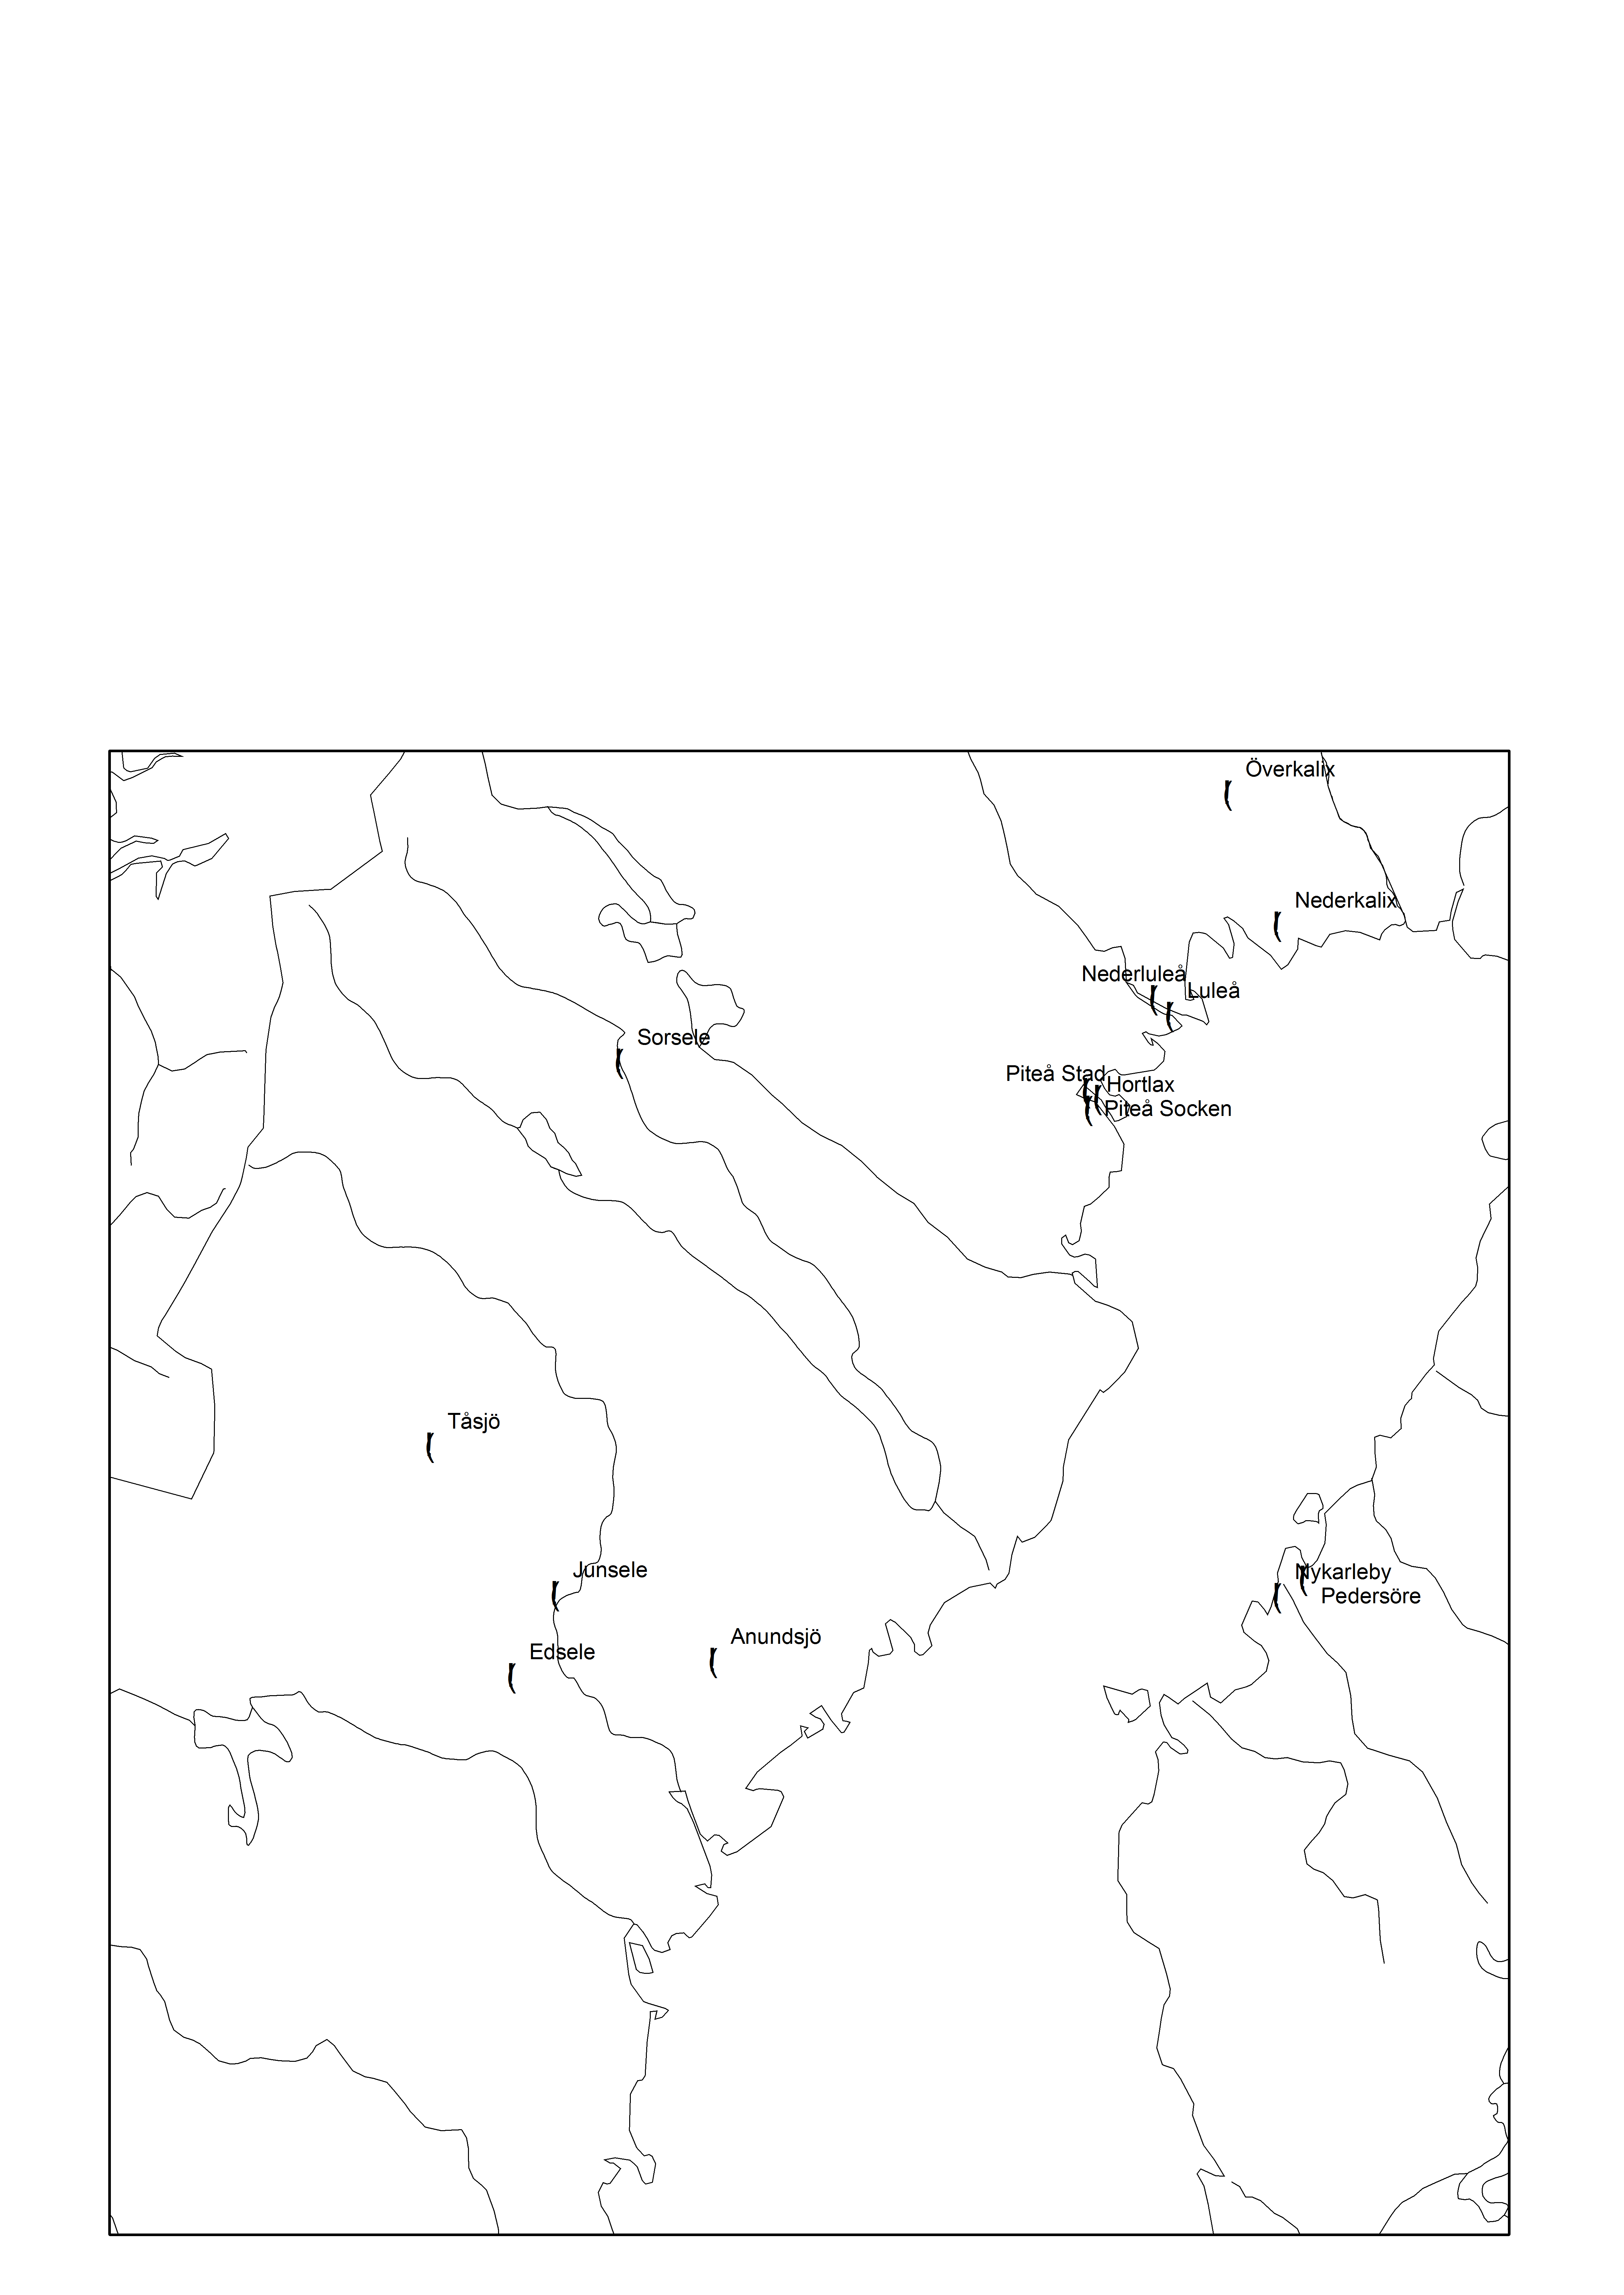
\includegraphics[height=.5\textheight]{figures/15_AttestationsofDefinites}
\caption{Attestations of definites after ‘much’.}
\label{map:12}

\end{figure}

\begin{figure}[h]

\includegraphics[height=.5\textheight]{figures/16_AttestationsofDefinitesNumerals}
\caption{Attestations of definites after numerals.}
\label{map:13}

\end{figure}

\begin{figure}[h]
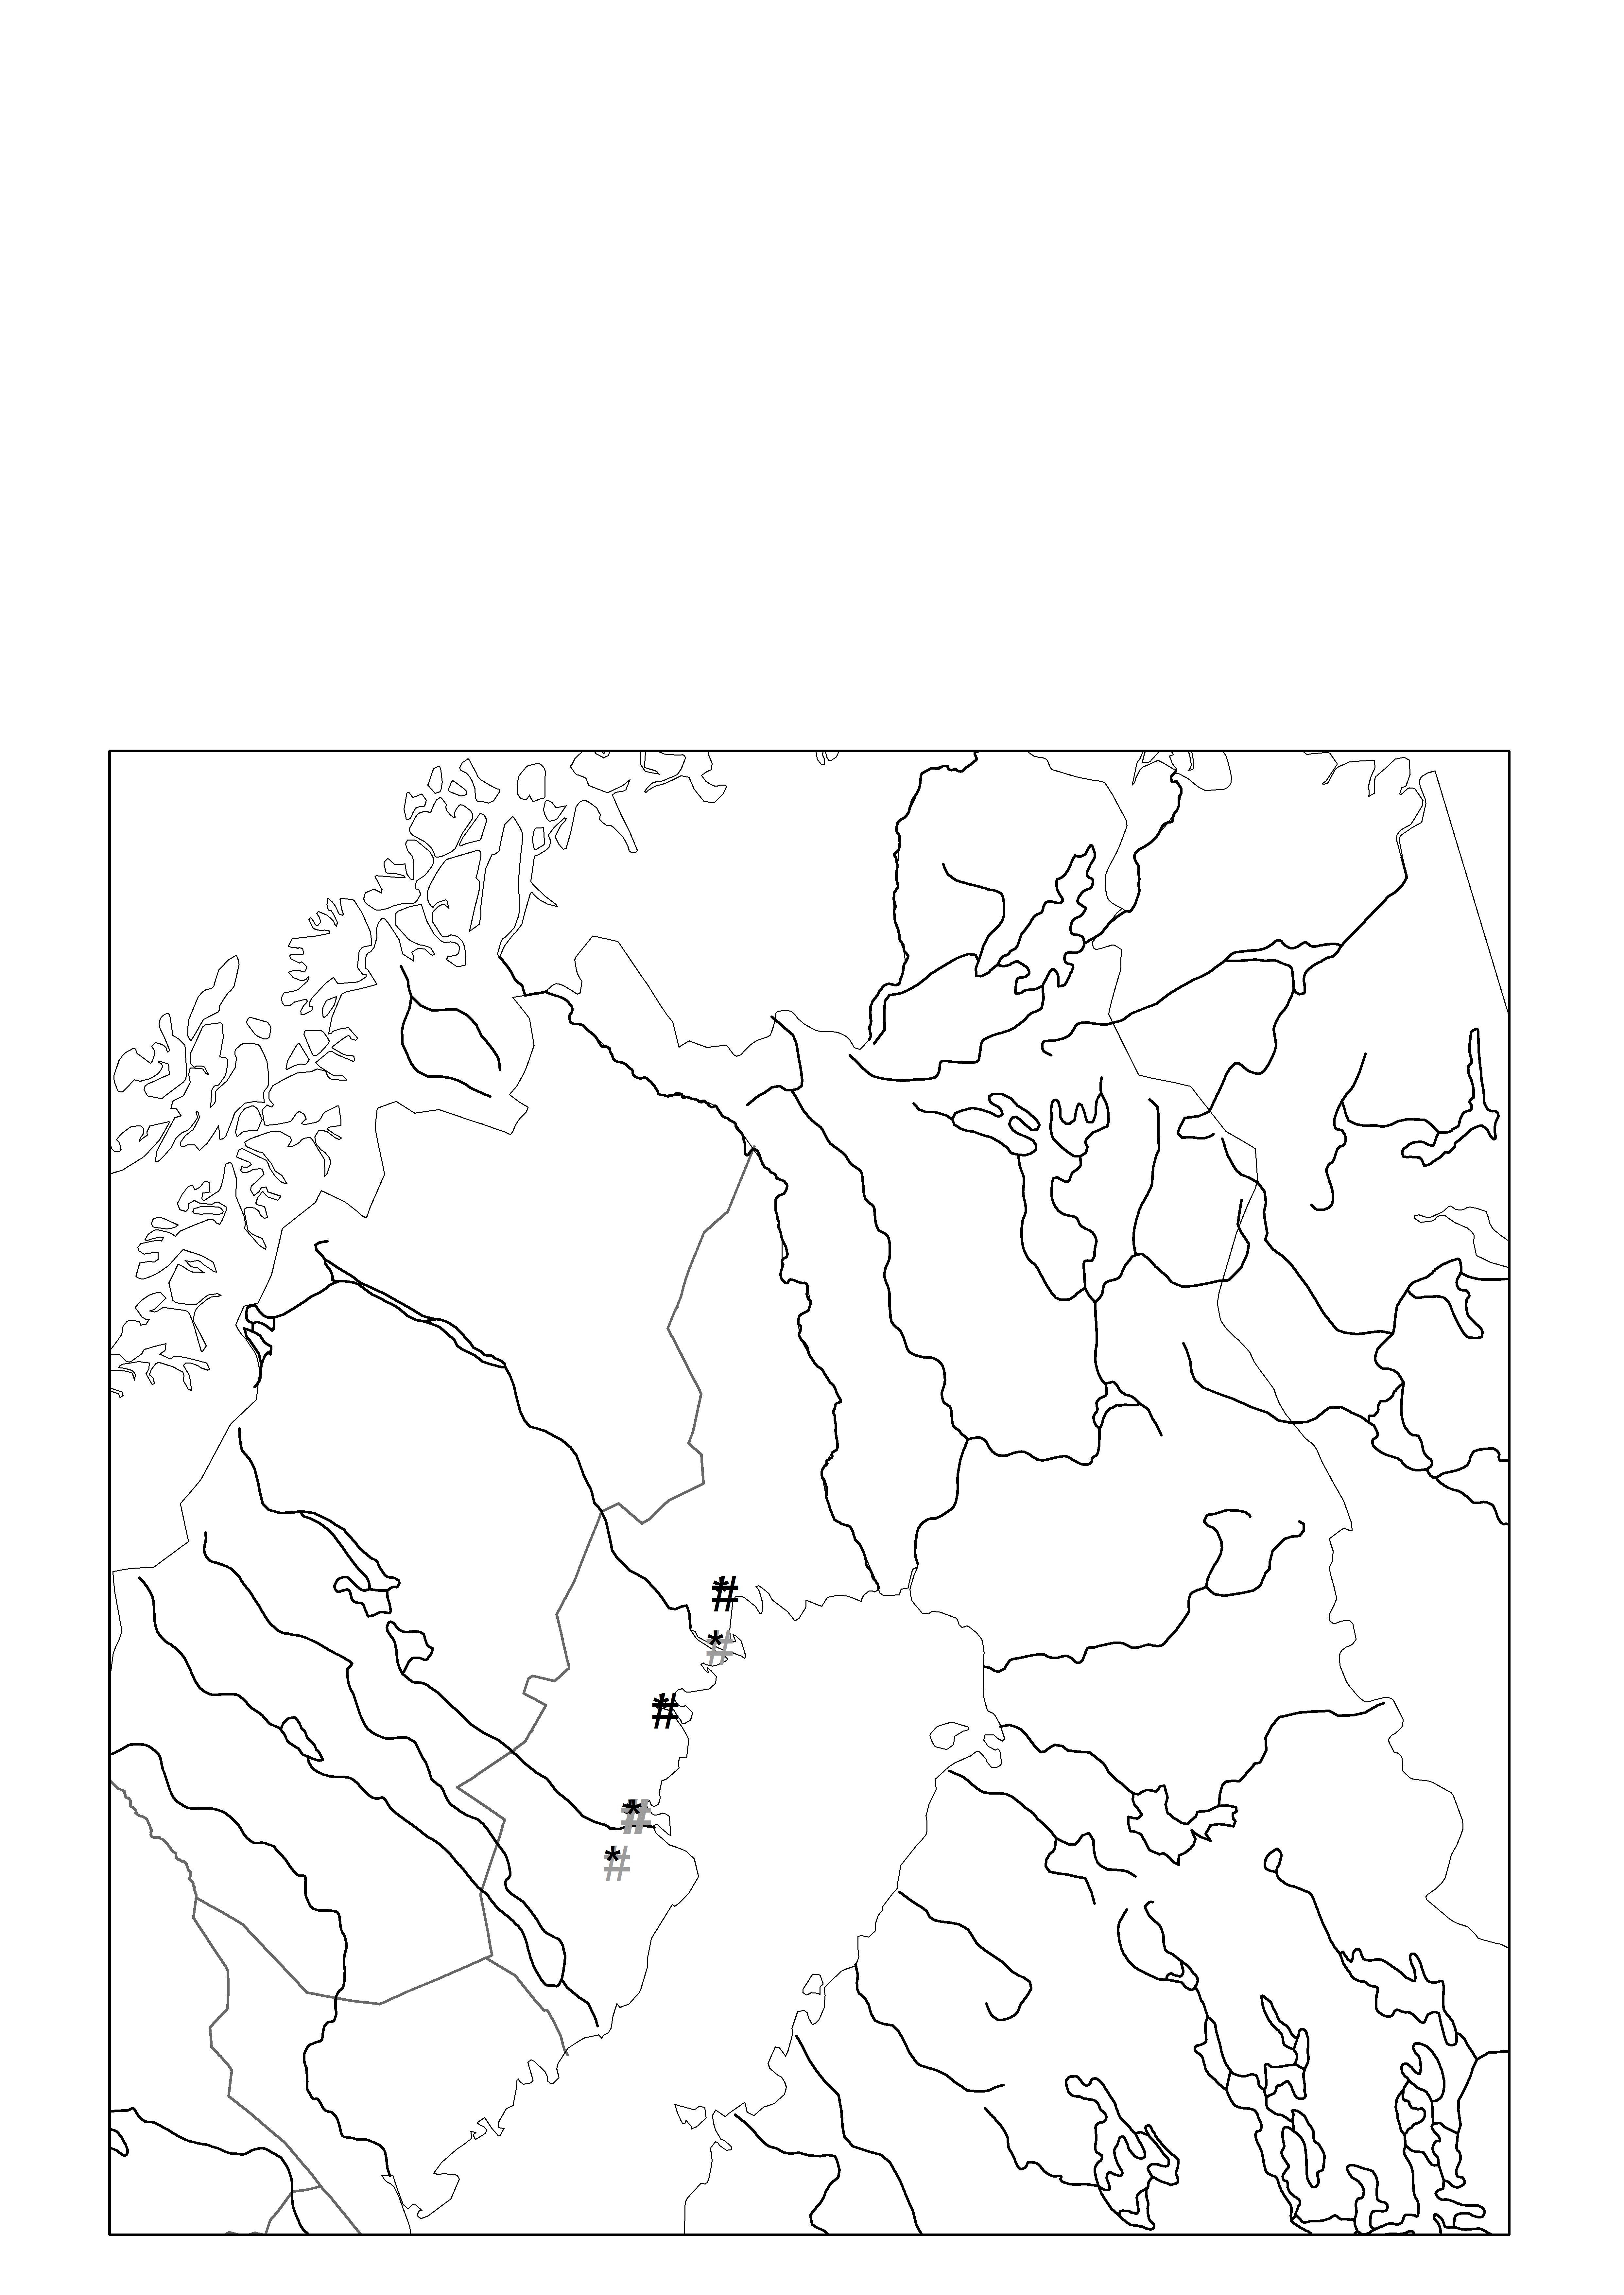
\includegraphics[height=.5\textheight]{figures/18_AttestationsofDatives}
\caption{Attestations of dative after quantifiers (black symbols: extended uses).}
\label{map:14}

\end{figure}

\begin{figure}[h]
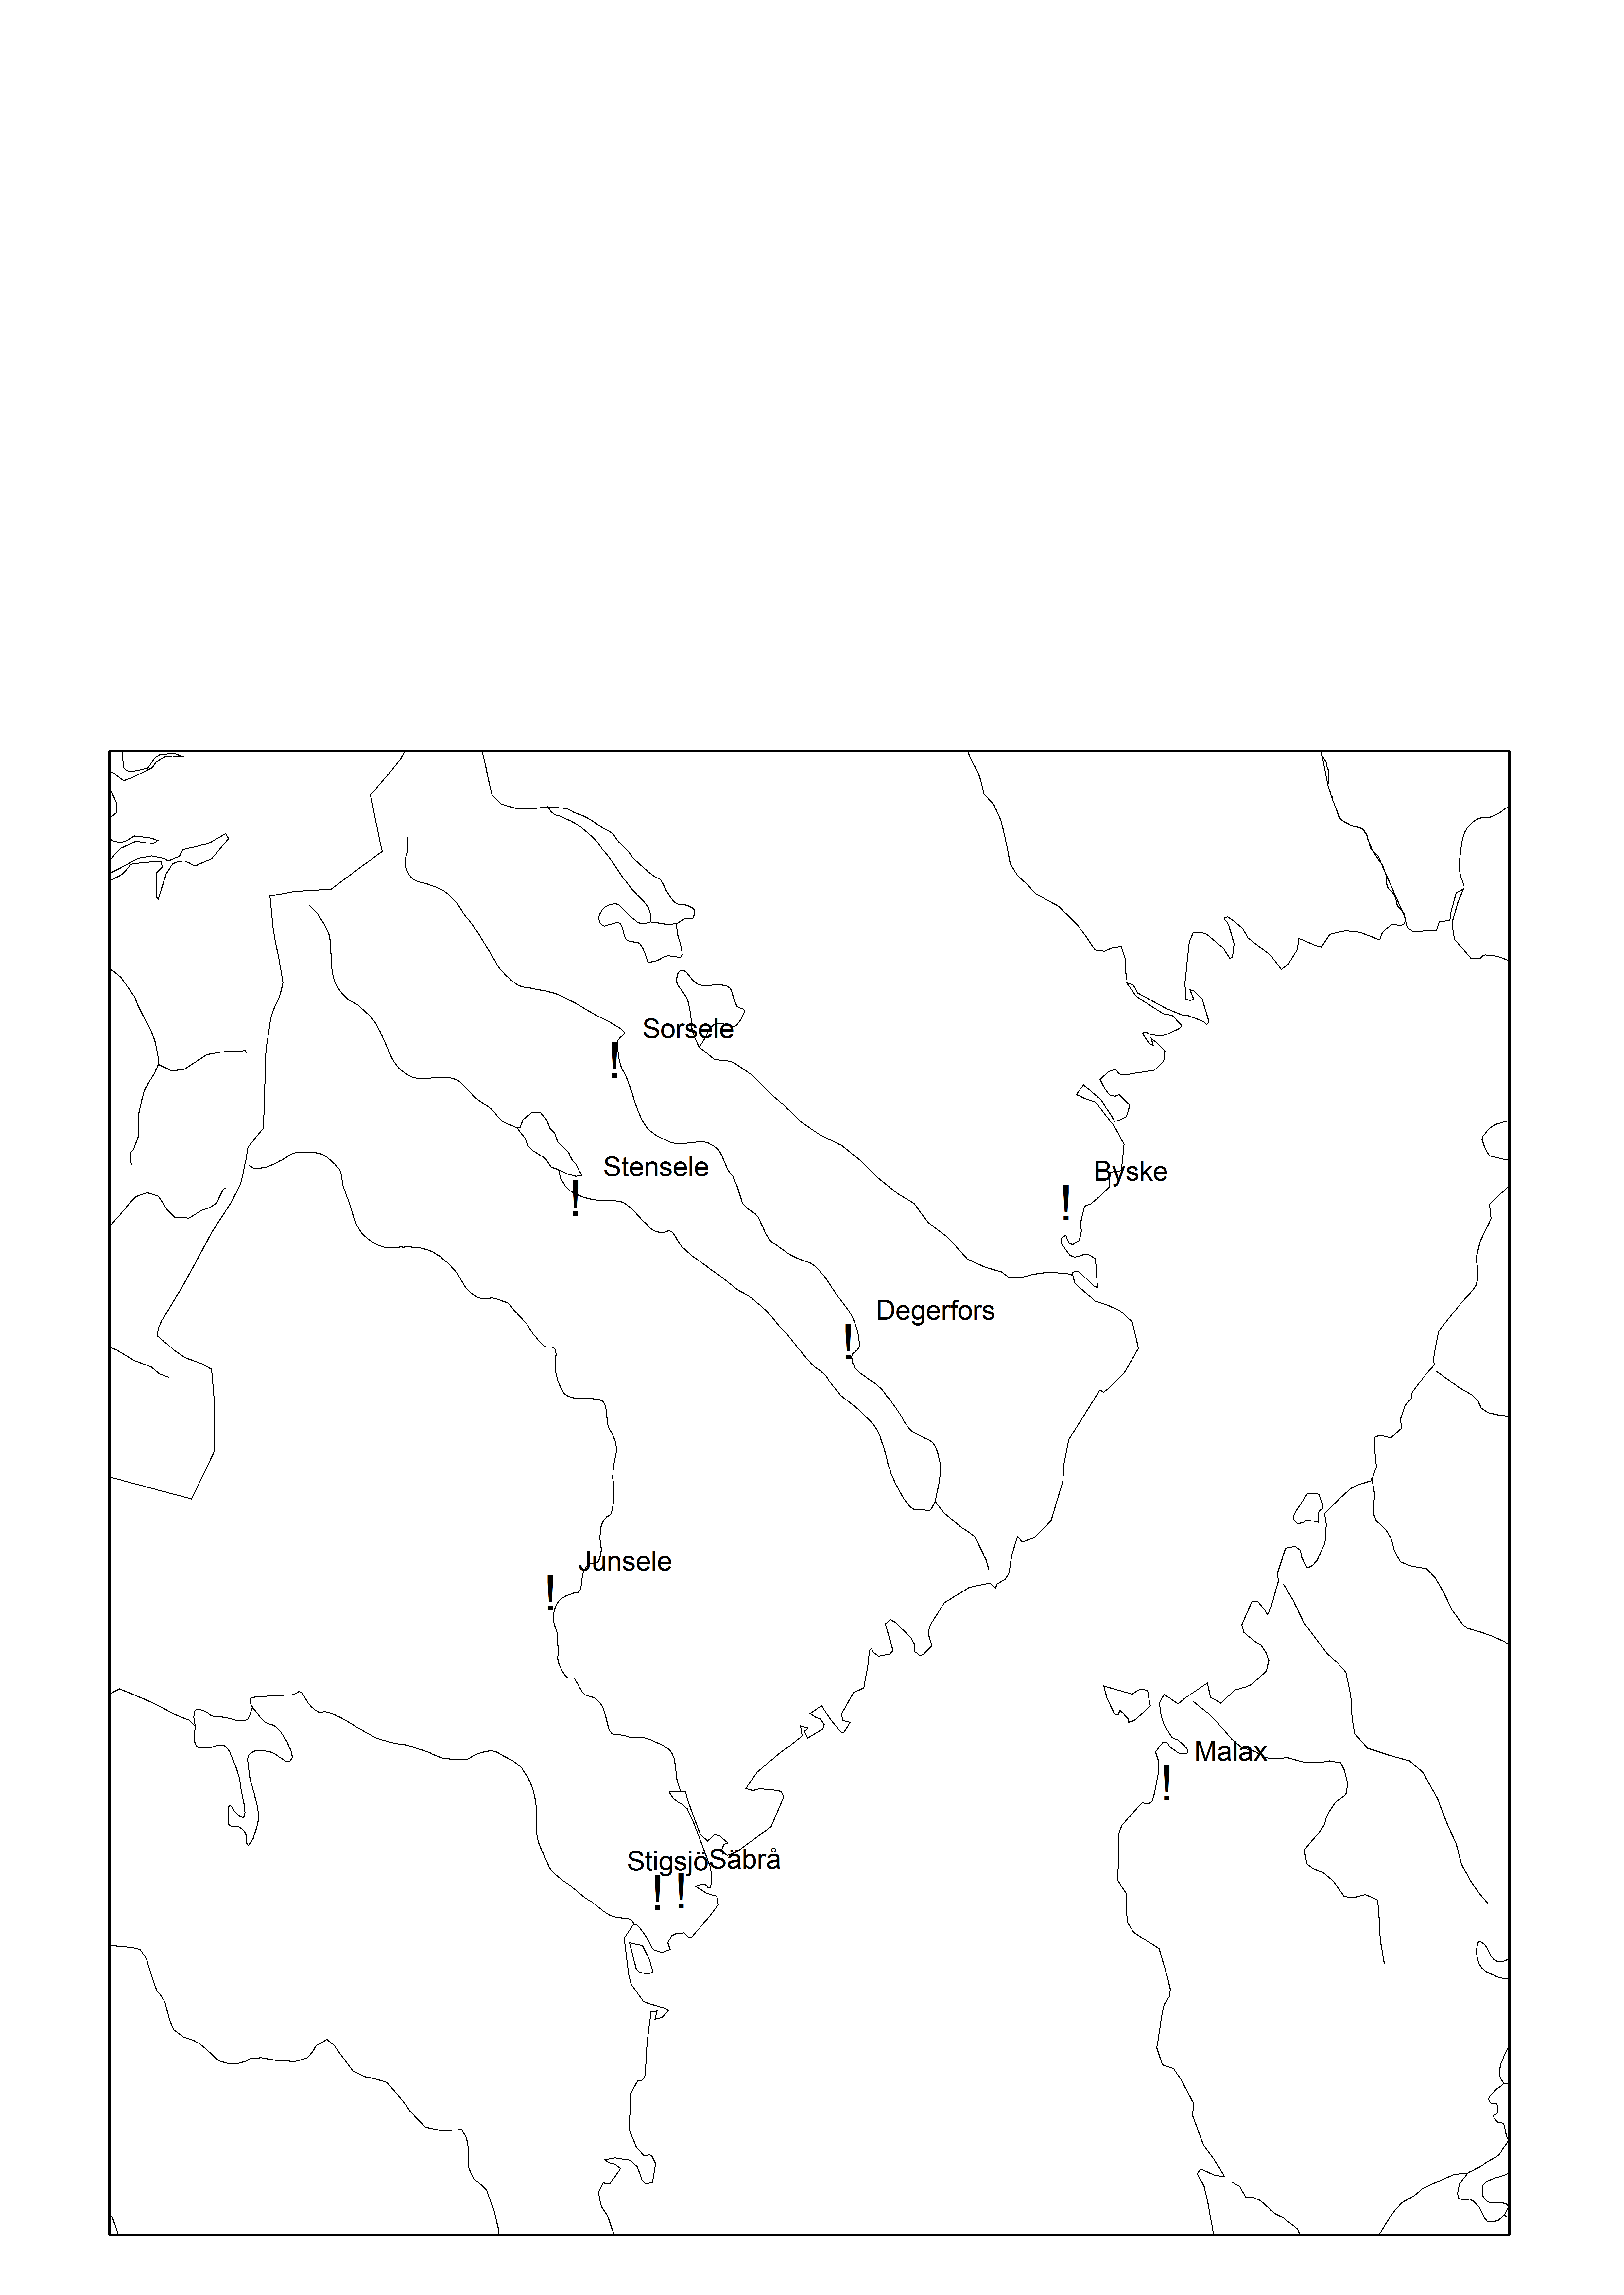
\includegraphics[height=.5\textheight]{figures/17_AttestationsAfterNa}
\caption{Attestations of definites after \textit{na}.}
\label{map:15}

\end{figure}

\subsection{ Singular count uses}
\label{sec:3.2.5}

In the peripheral area, there are also some unexpected uses of suffixed articles with singular count nouns, such as the following:

\ea \label{} 
\langinfo{\label{bkm:Ref224102863}Älvdalen (Os)}{}{}\\
\gll Am  \textbf{est-n.}\\
have.1{\pl}  \textbf{horse-{\deff}}\\
\glt ‘We have a horse, i.e. we are horse-owners.’ (questionnaire)

\z

Such examples, which would normally take an indefinite article in English, by and large correspond to “bare nouns” in the Central Scandinavian languages e.g.

\ea \label{} 
\langinfo{\label{bkm:Ref224102890}Swedish}{}{}\\
\gll Vi  har  \textbf{häst.}\\
we  have.{\prs}  \textbf{horse}\\
\glt ‘We have a horse, i.e. we are horse-owners.’

\z

I shall call such cases “low referentiality uses” (\citet[3:56]{TelemanEtAl1999}) “svagt referentiell betydelse”), since they share the trait that the identity of the referent is not highlighted; what is important in \REF{104}{}-\REF{105} is rather the property of owning a horse. Correspondingly, the bare noun construction in Swedish is normally used when speaking of something that it is normal to have exactly one exemplar of, including cars\footnote{ A Google search suggests that the bare noun phrase \textit{har bil} ‘has car’ is about ten times as common as \textit{har en bil} ‘has a car’ in Swedish, and of the latter the overwhelming majority were followed by a relative clause. } and telephones (at least until recently!), but excluding spaceships (because you are not expected to have one) or books (because you are expected to have several). However, the corresponding sentences with indefinite articles are also grammatical, and in fact preferred in certain contexts, e.g. if the referent is going to be important in the ensuing discourse. The articleless variant is however felt to be ungrammatical in Elfdalian (I have not been able to systematically check on other vernaculars), but conversely, the definite article is not possible in Central Scandinavian. 

From the diachronic point of view, the article-less cases of Central Scandinavian could be seen as due to an incomplete grammaticalization of the indefinite article, whereas the use of the definite article in Peripheral Swedish vernaculars is a case of grammaticalization that goes further than we would perhaps expect. Typologically, it is not wholly unique, however. While \REF{104} could not be translated into French using a definite article, there are similar examples such as \REF{106}, where a definite article is normal:

\ea \label{} 
\langinfo{\label{bkm:Ref224102943}French}{}{}\\
\gll Nous  avons  \textbf{le} \textbf{téléphone.}\\
we  have.{\prs}.1{\pl}  \textbf{{\deff}} \textbf{telephone}\\
\glt ‘We have a (lit. the) telephone.’

\z

Cases like this are mentioned in standard grammars of French, but they tend to be subsumed under generic uses of the article (I’ll return to this question in \sectref{sec:3.4}). 

With respect to the peripheral Swedish dialect area, the low referentiality uses of definite forms are not well documented in the literature, and when examples are provided they are usually not seen as a type of their own, distinct from non-delimited uses. For instance, \citet[282]{ÅgrenEtAl1954}, after discussing uses of definite forms for “indefinite quantities” and saying that Norrlandic dialects “are very consistent in this use of the definite forms”, cite the following as “maybe particularly striking to a Standard Swedish ear”:\footnote{ “De norrländska bygdemålen är mycket konsekventa i detta bruk av bestämd form. Särskilt påfallande för ett rikssvenskt öra är måhända…”} 

\ea \label{} 
\langinfo{Vilhelmina (SVb)}{}{}\\
\gll Sä  vi  mâka  ôss  \textbf{kâmmarn.}\\
so  we  clear.{\pst}  us  \textbf{chamber.{\deff}}\\
\glt ‘so we cleared us a chamber.’ [i.e. we made a shelter by clearing some snow]’

\z

This example, like the following ones, shows that the phenomenon may include cases that do not correspond to bare-noun constructions in Swedish: 

\ea\label{}
\langinfo{Älvdalen (Os)}{}{}\\
\gll E  wa  \textbf{swaindjin} å  weem.\\
it  be.{\pst}  \textbf{bend.{\deff}} on  road.{\deff}.{\dat}\\
\glt ‘There was a bend in the road.’ [S12]

\z

\ea
\gll Ig  ar  gart  \textbf{stark-äln} ig.\\
I   have.{\prs}  make.{\supp}  \textbf{strong\_heel.{\deff}.{\acc}} I\\
\glt ‘I have made a strong heel’ (\citet[95]{Levander1909})

\z

Due to restricted documentation and a rather low text-frequency, it is not so easy to establish the precise geographical distribution for the extended use of definite forms of singular count nouns, but I have found a number of examples from various ends of the Peripheral Swedish area, to be listed in the following: 

\subsubsection{Norrbothnian}
 Starting from the north, the following two translations of the same sentence from the Cat Corpus can be cited from the Kalix area:

\ea\label{}
\langinfo{Överkalix (Kx)}{}{}\\
\gll Ji  skå  taLa  om  föR  di  mamm\\
I  shall.{\prs}  speak.{\inf}  about  for  you.{\obl}  mother\\
\gll aT  ji  ållti  hä  önske  mi  i  kätt,\\
that  I  always  have.{\prs}  want.{\supp}  me.{\obl}  {\indf}  cat\\
\gll men  he  gär  jåo  äint  änn  aT  ha  \textbf{kätta}\\
but  it  go.{\prs}  {\prag}  {\neg}  well  {{\inf}m}  have.{\inf}  \textbf{cat.{\deff}}\\
\gll da´n  båo  ini  in  höires-häos.\\
when\_one  live.{\prs}  in  one.{\dat}.{\n}  apartment house\\
\glt ‘I want to tell you, Mother, that I have always wanted to have a cat – but it isn’t possible to have a cat (lit. the cat) when you live in an apartment house.’ (Cat Corpus)

\z

\ea\label{}
\langinfo{Nederkalix (Kx)}{}{}\\
\gll Jä  skå  tåla  åom  för  dä,  måmme\\
I  shall.{\prs}  speak.{\inf}  about  for  you.{\obl}  mother\\
\gll åt  jä  ållti  veillt  hå  i  kjaatt\\
that  I  always  want.{\supp}  have.{\inf}  {\indf}  cat  \\
\gll män  hä  gja  jo  ät  håå  \textbf{kjatta}\\
but  it  go.{\prs}  {\prag}  {\neg}  have.{\inf}  \textbf{cat.{\deff}}\\
\gll når  man  båo   ini  i  höreshöus.\\
when  one  live.{\prs}  in  {\indf}  apartment house\\
\glt (same translation as above)

\z

In \citet{Stenberg1971}, we find the following examples:

\ea\label{}
\langinfo{Siknäs, Nederkalix (Kx)}{}{}\\
\gll\bfseries
He  fanns  jo  separatoN.\\
\bfseries
it  exist.{\pst}  {\prag}  separator.{\deff}\\
\glt ‘There was a milk separator.’ 

\z

\ea\gll\bfseries
Jåå,  hästn  har  ve  jo.\\
\bfseries
yes  horse.{\deff}  have.{\prs}  we  {\prag}\\
\glt ‘Yes, we do have a horse.’ 

\z

A transcribed text on the DAUM website contains a couple of clear examples from the \textit{Lulemål} area (female speaker born in 1895):

\ea \label{} 
\langinfo{Edefors (Ll)}{}{}\\
\gll Vi  hadd  ju  åt  \textbf{j}\textit{än} \textbf{spisn} så\\
we  have.{\pst}  {\prag}  {\neg}  \textbf{iron\_stove.{\deff}} so\\
\gll en  kodd  ju  åt  b\textit{a}ka  bulla….\\
one  can.{\pst}  {\prag}  {\neg}  bake.{\inf}  bun.{\deff}.{\pl}\\
\gll Da  ve  fikk  \textbf{j}\textit{ä} \textbf{nspisn}\\
when  we  get.{\pst}  \textbf{iron\_stove.{\deff}}\\
\gll da  baka  ja  ju  wettbulla  å  pepark\textit{a}kun\\
then  bake.{\pst}  I  {\prag}  wheat\_bun.{\deff}.{\pl}  and  ginger-bread.{\deff}.{\pl}\\
\gll men  strakks  hadd  ve  barra  \textbf{öppenspisn.}\\
but  right\_away  have.{\pst}  we  only  \textbf{open\_stove.{\deff}}\\
\glt ‘As you know, we didn’t have an iron stove so we couldn’t bake buns… When we got an iron stove I used to bake wheat buns and gingerbreads, but in the beginning we had only an open fireplace.’ [S33]

\z

\subsubsection{Westrobothnian}
 In Västerbotten, there seems to be more variation in the use of singular count uses of definites than is found for non-delimited uses. Thus, \citet{BergholmEtAl1999} report that mainly older speakers used definite forms in \REF{112}. \citet{WälchliEtAl1998}, on the other hand, did not find any examples of definites at all in this sentence when using the same questionnaire.

\ea \label{} 
\langinfo{\label{bkm:Ref224103495}Burträsk (NVb)}{}{}\\
\gll Vi  hadd  \textbf{hästn} menn  ja  vor  litn.\\
we  have.{\pst}  \textbf{horse.{\deff}} when  I   be.{\pst}  small\\
\glt ‘We had a horse when I was a kid.’ (questionnaire)

\z

In transcribed texts from Västerbotten, a few examples are found, e.g.:

\ea \label{} 
\langinfo{Norsjö (NVb)}{}{}\\
\gll …å  för-ɭɑ’ɑi̯ŋ  se´nn  där-ɖäm  inte  hɑ’ɑdd  \textbf{tjö’ttkwɑ’ɳɑ}\\
and  for long  ago  where they  {\neg}  have.{\pst}  \textbf{meat-grinder.{\deff}}\\
\gll se  ɑ’nnvä’nnde  däm \textbf{kƚe’sta’i̯t’n.}\\
so  use.{\pst}  they  \textbf{“clothes-poker”.{\deff}}\\
\glt ‘…and long ago where they didn’t have a meat-grinder they used a \textit{klädstöt}.\footnote{ Tool used when washing clothes.} (\citet[303]{Westerberg2004})

\z

\ea \label{} 
\langinfo{\textit{Skelletmål} (NVb)}{}{}\\
\gll Hänna  dug  äint  för  ajn  som  ha  \textbf{julpän.} \\
this  do.{\prs}  {\neg}  for  one  that  have.{\prs}  \textbf{fly.{\deff}} \\
\glt ‘This won’t do for someone with a fly.’ (\citet[94]{Westerlund1978})

\z

\subsubsection{Middle Norrland}
 There seem to be no clear examples from the provinces of Jämtland, Ångermanland, and Medelpad. Although it is hard to argue from the absence of evidence, something could certainly be expected to show up in the extensive text materials, so it would appear that singular count uses are not found here. This impression is strengthened by the fact that definite forms are also not found with instrumental prepositional phrases (see below). 

\subsubsection{Ostrobothnian}
 \citet[207]{Nikula1997} quotes the following examples from Närpes, exemplifying the bare noun pattern:

\ea\label{}
\langinfo{Närpes (SOb) }{}{}\\
\gll Vi  ha:  \textbf{häst} därhäim.\\
we  have.{\prs}.{\pl}  \textbf{horse} at\_home\\
\glt ‘We have a horse at home.’

\z

\ea
\gll Ja  ha:r  no:  \textbf{moånanslyö:n.}\\
I  have.{\prs}  certainly  \textbf{monthly\_salary}\\
\glt ‘Sure, I have a monthly salary.’

\z

She seems to imply that this is the only possibility in this vernacular and explains this by the “non-referential function” of the noun phrases in question, which do not introduce a referent but rather contribute to the characterization of the subject as horse-owners and salaried employees respectively. 

\citet{ErikssonEtAl1999}, in their questionnaire investigation of Ostrobothnian, also found that the bare noun pattern was predominating. However, one informant from Munsala in northern Österbotten did produce a definite variant, together with one with an indefinite article:

\ea 
\langinfo{Munsala (NOb)}{}{}\\
	\ea { 
	\gll 	Vi  had  \textbf{hästin,} tå  ja  va  lill.\\
			we  have.{\pst}  \textbf{horse.{\deff}} when  I   be.{\pst}  small\\
	}
	\ex {
	\gll 	Vi  had  \textbf{in} \textbf{häst,} tå  ja  va  lill.\\
			we  have.{\pst}  \textbf{{\indf}} \textbf{horse} when  I  be.{\pst}  small\\
	\glt 	‘We had a horse when I was a kid.’ (questionnaire)
	}
	\z 
\z

\citet{ErikssonEtAl1999} a\textstyleBodyTextFirstChar{l}so quote a number of examples of definite-marked countable singulars from published texts:

\ea \label{} 
\langinfo{Sideby (SOb)}{}{}\\
\gll Så  kviila  vi  \textbf{middain.} \\
so  rest.{\pst}  we  \textbf{noon.{\deff}} \\
\glt ‘Then we took a nap.’ (Standard Swedish \textit{vila middag}) [S19]

\z

\ea \label{} 
\langinfo{Sideby (SOb)}{}{}\\
\gll Å  dåm  hav  \textbf{öitjon.}\\
and  they  have.{\prs}  \textbf{dinghy.{\deff}}\\
\glt ‘And they have a dinghy.’ [S19]

\z

\citet{Ivars2005} presents at least one fairly clear example from Närpes:

\ea \label{} 
\langinfo{Närpes (SOb)}{}{}\\
\gll Han  ha:  ju  \textbf{brännvinsbo:den} han.  \\
he  have.{\pst}  {\prag}  \textbf{liquor-shop.{\deff}} he  \\
\glt ‘He had a liquor shop, he.’ 

\z

Thus, the use of definite forms with singular countables is fairly well documented also in Ostrobothnian, although the article-less pattern is more common in present-day usage.

\textbf{Ovansiljan}. Examples from Elfdalian have already been quoted above. Questionnaires from Orsa and Sollerön give a result which is similar to the one reported above for non-delimited uses. Thus, the majority of the informants from Orsa used the definite form in \REF{120}, whereas none from Sollerön did:

\ea \label{} 
\langinfo{\label{bkm:Ref224103820}Orsa (Os)}{}{}\\
\gll Wi  addum  \textbf{äst’n} dö  i  wa  lit’n.\\
we  have.{\pst}.1{\pl}  \textbf{horse.{\deff}} when  I   be.{\pst}  small\\
\glt ‘We had a horse when I was a kid.’ (questionnaire)

\z

\subsubsection{Summing up}
 Like the use of definite forms after quantifiers, the extended use of definite forms with count nouns display is less well entrenched in the Peripheral Swedish area than the non-delimited type. Their absence from the Middle Norrland area is conspicuous. (Compare also the more questionable example \REF{188} from Hållnäs in Uppland below.)

\subsection{ Instrumental prepositional phrases }

\citet{Himmelmann1998} claims that articles “are generally used less frequently, and with regard to semantic and pragmatic generalisations, less consistently in adpositional phrases than in other syntactic environments (such as subject or object position)”. Manner and instrumental adverbial phrases would be a case in point, and indeed, in English, certain types of manner-characterizing prepositional phrases tend to involve bare nouns, particularly those that indicate manner of locomotion, such as \textstyleLinguisticExample{by train}, \textstyleLinguisticExample{by foot}, \textstyleLinguisticExample{by car}. In Central Scandinavian, the use of such bare nouns is considerably wider. Thus, in Swedish, the phrase \textstyleLinguisticExample{med kniv} ‘[lit.] with knife’ is much more common\footnote{ A Google count: \textit{med}\textit{ }\textit{kniv}: 14300, \textit{med en kniv}: 2820. In English, there is a parallel in the phrase \textit{by} \textit{knife}, appearing in phrases such as \textit{homicide by knife}.} than \textstyleLinguisticExample{med en kniv }‘with a knife’, and in the following sentence, the use of an indefinite article sounds definitely strange:

\ea \label{} 
\langinfo{\label{bkm:Ref224115033}Swedish}{}{}\\
\gll Hon  äter  soppa  med  \textbf{(?en)} \textbf{  sked.}\\
she  eat.{\prs}  soup  with  \textbf{{\indf}} \textbf{spoon}\\
\glt ‘She eats soup with a spoon.’

\z

In the light of these observations and Himmelmann’s claim, it is rather unexpected to find languages where in fact \REF{121} would be translated using a definite article in the phrase ‘with a spoon’, even when it is evident that no specific spoon is being referred to. Nevertheless, in French, if the preposition \textstyleLinguisticExample{à} is chosen, it is regularly followed by the definite rather than by the indefinite article:

\ea \label{} 
\langinfo{French}{}{}\\
\gll Elle  mange  la  soupe  à  \textbf{la} \textbf{cuillière.}\\
she  eat.{\prs}  {\deff}  soup  with  \textbf{{\deff}} \textbf{spoon}\\
\glt ‘She eats soup with a spoon.’

\z

where a definite NP is used after the preposition \textstyleLinguisticExample{à}. With this preposition, the definite article seems more or less obligatory. (Compare captions of paintings such as \textstyleLinguisticExample{Jeune fille au chèvre} ‘Young girl with a goat’). With the synonymous preposition \textstyleLinguisticExample{avec} the definite article is possible but the preferred variant appears to be with an indefinite NP:

\ea \label{} 
\langinfo{French}{}{}\\
\gll Elle  mange  la  soupe  avec  \textbf{une} \textbf{cuillière.}\\
she  eat.{\prs}  {\deff}  soup  with  \textbf{{\indf}} \textbf{spoon}\\
\glt ‘She eats soup with a spoon.’

\z

Similarly, in the Peripheral Swedish vernaculars, instrumental phrases of this type often show up with a definite head noun. Thus, \citet[126]{Levander1909} quotes the following Elfdalian example, which he translates into Swedish using a bare noun construction (\textstyleLinguisticExample{med kniv} ‘with a knife’)

\ea \label{} 
\langinfo{Älvdalen (Os)}{}{}\\
\gll Sjo  ur  dier  ovo  skrievað  \textbf{min} \textbf{  knaivem!}\\
see  how  they  have.{\prs}.3{\pl}  write.{\supp}  \textbf{with} \textbf{knife.{\deff}.{\dat}}\\
\glt ‘Look what they have written with a knife!’ (\citet[125]{Levander1909})

\z

%\begin{styleTextkrper}
A modern Elfdalian example elicited by questionnaire is \REF{125}.

%\end{styleTextkrper}

\ea \label{} 
\langinfo{\label{bkm:Ref224103303}Älvdalen (Os)}{}{}\\
\gll An  jät  supp\k{u}  \textbf{min} \textbf{  stjiedn.}\\
he  eat.{\prs}  soup.{\deff}.{\acc}  \textbf{with} \textbf{spoon.{\deff}.{\dat}}\\
\glt ‘He eats soup with a spoon.’ (questionnaire)

\z

%\begin{styleTextkrper}
However, the informant indicated that the indefinite form was also possible:

%\end{styleTextkrper}

\ea \label{} 
\langinfo{Älvdalen (Os)}{}{}\\
\gll An  jät  supp\k{u}  \textbf{min} \textbf{  stjied.}\\
he  eat.{\prs}  soup.{\deff}.{\acc}  \textbf{with} \textbf{spoon.{\dat}}\\
\glt ‘He eats soup with a spoon.’ (questionnaire)

\z

%\begin{styleTextkrper}
From Orsa, where there were several questionnaire responses, the majority used a definite form, either in the dative or non-case marked:

%\end{styleTextkrper}

\ea \label{} 
\langinfo{Orsa (Os)}{}{}\\
\gll An  jat  suppo  \textbf{mi} \textbf{  stjed’n/stjedi.}\\
he  eat.{\prs}  soup.{\deff}.{\acc}  \textbf{with} \textbf{spoon.{\deff}}\\
\glt ‘He eats soup with a spoon.’ (questionnaire)

\z

%\begin{styleTextkrper}
Out of four questionnaire responses from Sollerön, a definite form was given by all three informants born before 1940:

%\end{styleTextkrper}

\ea \label{} 
\langinfo{Sollerön (Os)}{}{}\\
\gll An  jät  såppo  \textbf{minn} \textbf{  stjedn.} \\
he  eat.{\prs}  soup.{\deff}.{\acc}  \textbf{with} \textbf{spoon.{\deff}} \\
\glt ‘He eats soup with a spoon.’ (questionnaire)

\z

For Upper Norrland, we find definite forms throughout, as evidenced in questionnaires from Bjurholm, Burträsk, Norsjö, and Glommersträsk:

\ea \label{} 
\langinfo{Bjurholm (NVb)}{}{}\\
\gll Han  ät  soppa  \textbf{ve} \textbf{skea.} \\
he  eat.{\prs}  soup.{\deff}  \textbf{with} \textbf{spoon.{\deff}} \\
\glt ‘He eats soup with a spoon.’ (questionnaire)

\z

In an early text from Överkalix, the following example is found:

\ea \label{} 
\langinfo{Överkalix (Kx)}{}{}\\
\gll …fistsen  fik  di  takkɷ  åys  ɷpp\\
fish.{\deff}  get.{\pst}  they  almost  scoop.{\inf}  up\\
\gll \textbf{ve} \textbf{slaiven} bårti  anɷ…\\
\textbf{with} \textbf{ladle.{\deff}} from  river.{\deff}\\
\glt ‘…as for the fish, they almost had to scoop it up with a ladle from the river…’ [S17]

\z

Similar examples are found in other transcribed texts from Överkalix. 

\subsubsection{Middle Norrland}
 No examples have been found in texts from Jämtland, Ångermanland, and Medelpad. For Jämtland, informants from Lit indicate that definite forms are not possible in examples of this type.

\subsubsection{Ostrobothnian}
\citet{Hummelstedt1934} enumerates quite a few examples of the type from Närpes. 

	
\ea\label{}
\langinfo{Närpes (SOb)}{}{}\\
	\ea {
	\gll 	Vi  sk\=ar  a  \textbf{me} \textbf{štjeron.} \\
			we  cut.{\pst}  it  \textbf{with} \textbf{sickle.{\deff}} \\
			
	\glt ‘We cut it with a sickle.’
	}
	\ex {
	\gll 	Vi  $\lambda $\=ow  \textbf{me} \textbf{lijjan.} \\
			we  cut.{\pst}  \textbf{with} \textbf{scythe.{\deff}} \\
	\glt 	‘We cut [grass] with a scythe.’
	}
	\ex {
	\gll 	Ja  tju\={ö}p  \textbf{me} \textbf{tjärron.} \\
			I  drive.{\pst}  \textbf{with} \textbf{cart.{\deff}} \\
	\glt 	‘I drove [with] a cart.’ 
	} 
	\ex {
	\gll	He  ji\=eg  me  $\lambda$ edan.\\
			it  go.PRET  \textbf{with} \textbf{sledge.{\deff}}\\
	\glt 	‘We went [lit. it went] by sledge.’ (\citet[135]{Hummelstedt1934})
	}
	\z 
\z

\citet{Ivars2005} gives examples such as \textstyleLinguisticExample{me} \textstyleLinguisticExample{kni:vin }‘with knife.{\deff}’, \textstyleLinguisticExample{me} \textstyleLinguisticExample{li:an} ‘with scythe.{\deff}’ from South Ostrobothnian. (\citet{Nikula1997}, who also discusses Närpesmål, does not mention instrumental phrases at all.)

In the translation of the sentence ‘He eats soup with a spoon’, \citet{ErikssonEtAl1999} obtained four definite-marked responses among a total of 11 Ostrobothnian informants:

\ea 
	\ea { \label{}
	\langinfo{Malax (SOb)}{}{}\\
	\gll 	Ha  jeter  soppu  \textbf{me} \textbf{  skeide.}\\
			he  eat.{\prs}  soup.{\deff}?  \textbf{with} \textbf{spoon.{\deff}}\\
	}
	\ex {
	\langinfo{Närpes (SOb)}{}{}\\
	\gll 	An  jäter  soppon  \textbf{me} \textbf{  sjöiden.}\\
			he  eat.{\prs}  soup.{\deff}  \textbf{with} \textbf{spoon.{\deff}}\\
	}
	\ex {
	\langinfo{Tjöck (SOb)}{}{}\\
	\gll 	Han  jiter  sopon  \textbf{me} \textbf{skeiden.}\\
			he  eat.{\prs}  soup.{\deff}  \textbf{with} \textbf{spoon.{\deff}}\\
	\glt 	‘He eats soup with a spoon.’
	}
	\z 
\z

They also quote the phrase \textstyleLinguisticExample{sloo me liian} ‘cut with a scythe’ from [S19]. 

Examples are also found in Southern Finland and Estonia, where extended uses of definites are in general quite restricted. Thus, \citet{Lundström1939} quotes examples from Nyland:

\ea\label{}
\langinfo{Snappertuna (Ny) }{}{}\\
\gll Man  sl\=or  gräse  \textbf{me} \textbf{l\={\i}an.}\\
one  cut.{\prs}  grass.{\deff}  \textbf{with} \textbf{scythe.{\deff}}\\
\glt ‘One cuts the grass with a scythe.’ (\citet[15]{Lundström1939})

\z

\ea
\gll Nɷ  bl\={\i}r  e  br\=a  dehäran,\\
sure  become.{\prs}  it  good  this\\
\gll bara  man  tar  innoger  t\=ag  \textbf{me} \textbf{hyviln.}\\
just  one  take.{\prs}  a\_few  take.{\pl}  \textbf{with} \textbf{plane.{\deff}}\\
\glt ‘This will surely be good, if you take a few shavings with a plane.’ (\citet[15]{Lundström1939})

\z

In a text from Ormsö in Estonia, we find the following example:

\ea \label{} 
\langinfo{Ormsö (Es)}{}{}\\
\gll Nu  kond  ve  bere  hlå  r\textit{å}gen  \textbf{mä} \textbf{l} \textbf{\textit{i}} \textbf{an}\\
now  can.{\pst}  we  begin.{\inf}  cut.{\inf}  rye.{\deff}  \textbf{with} \textbf{scythe.{\deff}}\\
\gll å  triske  bLai  nu  m\textit{i}ke  leta.\\
and  threshing  become.{\pst}  now  much   easy.{\cmpr}\\
\glt ‘‘Now we could begin to cut the rye with a scythe and the threshing became much easier.’ [S24]

\z

\subsubsection{Summing up}
 The use of definite forms in instrumental prepositional phrases can be considered a special case of uses with singular count nouns. The distribution of the instrumental use also is somewhat similar to that of definite forms in constructions such as ‘We have a horse’, discussed in \sectref{sec:3.2.5}. In particular, we may note that no attestations are found from Middle Norrland. On the other hand, the instrumental use extends to some areas where the other types of definite singular count nouns are not found, viz. southern Finland and Estonia. 

A possible objection (Ulrika Kvist Darnell, personal communication) is that the intended interpretation in the examples in this section is not indefinite but instead closer to something like ‘the X that I have’. It is true that if the examples had occurred in a text corpus, it would have been difficult to know exactly how they should be understood. However, the use of definites in such contexts has been noted as striking from the point of view of the standard language by several scholars who are well acquainted with the vernaculars in question. Many examples were also given as translations of Swedish sentences with indefinite noun phrases. But the fact that such examples have a somewhat fluid interpretation may be relevant in a diachronic context – see further the discussion in \sectref{sec:3.4}. 

\subsection{  “Det var kvällen”}
\label{sec:3.2.6}

\citet[16]{Delsing2003a} subsumes two different cases under “predicative constructions”: one exemplified by examples such as \textstyleLinguisticExample{hä ä sommarn} ‘it is summer’, which he calls “impersonal”, and another exemplified by “identifying constructions” such as 

\ea \label{} 
\langinfo{\label{bkm:Ref224115132}(no location)}{}{}\\
\gll De  här  ä  \textbf{körpen.}\\
this  here  be.{\prs}  \textbf{pick.{\deff}}\\
\glt ‘This is a pick.’

\z

It appears, though, that these two patterns have rather different geographic distributions. Examples like \REF{135}, which are rather close to citation uses (see \sectref{sec:3.2.1}), are not to my knowledge attested outside the area where extended uses of definites are normally found, but “impersonal” constructions characterized by the pattern

%\begin{styleBlockQuote}
impersonal subject ‘it’ + copular verb ‘be’ or ‘become’ + noun denoting a temporal interval

%\end{styleBlockQuote}

are quite widespread in Scandinavia. In the Swedish dialect area, examples can thus be found not only in Härjedalen, Västerdalarna, Dalabergslagen and Åboland, all close to the extended definite area, but also in south-western Sweden (the provinces of Halland and Bohuslän): 

\ea \label{} 
\langinfo{Träslövsläge (Hl)}{}{}\\
\gll Nu  borja  här  a  bli  \textbf{kwälen,} \\
now  begin.{\pst}  here  {{\inf}m}  become.{\inf}  \textbf{evening.{\deff}} \\
\gll a  sola  gick  nair  i  sjön.\\
and  sun.{\deff}  go.{\pst}  down  in  lake.{\deff}\\
\glt ‘Now evening was coming (lit. it started to become the evening), and the sun set in the lake.’ (Cat Corpus)

\z

\ea \label{} 
\langinfo{Sotenäs (Bo)}{}{}\\
\gll Dä  hôllte  pô  ô  b?i  \textbf{vårn} no,\\
it  hold.{\pst}  on  {{\inf}m}  become.{\inf}  \textbf{spring.{\deff}} now\\
\gll dä  kjännte  Pissen.\\
that  feel.{\pst}  pussycat.{\deff}\\
\glt ‘Spring was coming (lit. it was becoming spring), Cat felt that.’ (Cat Corpus)

\z

\ea \label{} 
\langinfo{Östmark (Vm)}{}{}\\
\gll Nu  ä  dä  snart  \textbf{sommarn.}\\
now  be.{\prs}  it  soon  \textbf{summer.{\deff}}\\
\glt ‘Now it will soon be summer.’ (\citet{Broberg1936})

\z

\ea \label{} 
\langinfo{Transtrand (Vd) }{}{}\\
\gll Hä  vaL  snart  \textbf{vintern.}\\
it  become.{\prs}  soon  \textbf{winter.{\deff}}\\
\glt ‘It will soon be winter.’ (questionnaire)

\z

\ea \label{} 
\langinfo{Houtskär (Åb)}{}{}\\
\gll N\=or  he  bǣ7ei  \textbf{kv} \textbf{\=e} \textbf{ldinj}\\
when  it  become.{\pst}  \textbf{evening.{\deff}}\\
\gll o  in  k\=om  heim  me  f\=orenj…\\
and  he  come.{\pst}  home  with  sheep.{\deff}.{\pl}\\
\glt ‘When evening came and he came home with the sheep…’ (\citet[38]{Lundell1936})

\z

Delsing mentions a Norwegian informant from Trøndelag who accepts examples of this type, giving the impression that it is locally restricted in Norwegian. In fact, the construction is well represented in written Norwegian, both Bokmål and Nynorsk. The following example is from the Nynorsk part of the “Norsk Tekstarkiv”: 

\ea \label{} 
\langinfo{Nynorsk Norwegian}{}{}\\
\gll Det vart  \textbf{kvelden} og  det  vart  \textbf{natta} på  nytt.\\ % \href{http://kh.hd.uib.no/cgi-dos/roman-nn.bat?P3C383000#here}{Det}
it  become.{\pst}  \textbf{evening.{\deff}} and  it  become.{\pst}  \textbf{night.{\deff}} on  new\\
\glt ‘Evening came and it became night again.’ [S29]

\z

%\begin{styleTextkrper}
An Internet example in Bokmål: 

%\end{styleTextkrper}

\ea \label{} 
\langinfo{Bokmål Norwegian}{}{}\\
\gll Da  det  ble  \textbf{kvelden} \\
when  it  become.{\pst}  \textbf{evening.{\deff}} \\
\gll hadde  bortimot  250  shaman’er\\
have.{\pst}  around  250  shaman.{\pl}\\
\gll samlet  seg  rundt  slangen  og  kvinnen…\\
collect.PP  {\refl}.3{\pl}  around  snake.{\deff}  and  woman.{\deff}\\
\glt ‘When evening came, around 250 shamans had collected around the snake and the woman…’ (Internet)

\z

The pattern does not seem to be possible in Danish or in the southernmost Swedish provinces (although it goes as far south as Halland). Its wide distribution makes it somewhat unlikely that it has spread together with the other extended uses of definite forms, which are less widespread. 

\subsection{ Various minor patterns}

\subsubsection{Illnesses}
 In the literature, names of illnesses are sometimes provided as examples where definite forms are used in vernaculars more extensively than in Swedish. Thus: 

\ea \label{} 
\langinfo{Pyttis (Ny) }{}{}\\
\gll Bɷonen  har  jɷ  \textbf{c(ikhɷston.}\\
child.{\deff}.{\pl}  have.{\prs}  {\prag}  \textbf{whooping-cough.{\deff}}\\
\glt ‘The children have got whooping-cough.’ (\citet[11]{Lundström1939})

\z

\ea \label{} 
\langinfo{Östmark (Vm)}{}{}\\
\gll Han  ä  ill  kommen  ta  \textbf{jekta.}\\
he  be.{\prs}  badly  come.PP  of  \textbf{gout.{\deff}}\\
  ‘He is suffering badly from gout’ (\citet{Broberg1936})
\z 
  
\ea \label{} 
\langinfo{Sollerön (Os) }{}{}\\
\gll I  a  fänndji  \textbf{ålldi.} \\
I  have.{\prs}  get.{\supp}  \textbf{stitch.{\deff}} \\
\glt ‘I have got a stitch in my side.’ (\citet[285]{AnderssonEtAl1999})

\z

It seems hard to generalize here, though, since names of illnesses tend to behave idiosyncratically in many languages, including English – thus, \textstyleLinguisticExample{flu} is preferably used with the article but the synonymous \textstyleLinguisticExample{influenza} without.

\textbf{Measure phrases}. Definite forms also sometimes show up in phrases denoting measurements of time, weight, etc. \citet[9]{Lundström1939} provides a number of examples from Nyland: 

\ea
	\ea {
	\langinfo{Pojo (Ny)}{}{}\\
	{}[Hur länge räcker det till Lovisa?]\\
	\gll 	\textbf{Timmen} o  femton.\\
			\textbf{hour.{\deff}} and  fifteen\\
	\glt 	‘[How far is it to Lovisa?] - One hour fifteen.’
	}
	
	\ex {
	\langinfo{Borgå (Ny)}{}{}\\
	\gll	Han  c(\={ö}rd  \textbf{på} \textbf{t} \textbf{\={\i}} \textbf{man.}\\
			he  drive.{\pst}  \textbf{on} \textbf{hour.{\deff}}\\
	\glt 	‘He drove [the distance] in an hour.’
	}
	\z
\z 
	
%\begin{styleTextkrper}
In the Cat Corpus, I have only found one clear example from Överkalix (all the other vernaculars have an indefinite NP in the corresponding sentence):

%\end{styleTextkrper}

\ea \label{} 
\langinfo{Överkalix (Kx) }{}{}\\
\gll He  dråo  nestan  \textbf{haL(e)v-täimen}\\
it  take.{\pst}  almost  \textbf{half-hour.{\deff}}\\
\gll enan  fressn  tåoRs  koma  främm.\\
before  tomcat.{\deff}  dare.{\pst}  come.{\inf}  fore\\
\glt ‘It took almost half an hour before Cat dared come out.’ (Cat Corpus)

\z

\subsection{ Preproprial articles}
\label{sec:3.2.8}

What is most appropriately called preproprial articles are used widely in Scandinavia. Preproprial articles are identical in form to third person pronouns – either full forms, which is common in Norway, or reduced (clitic) forms, as is the normal case in Sweden: \textstyleLinguisticExample{a Brita} ‘Brita’, \textstyleLinguisticExample{n Erik }‘Erik’. 

In most colloquial varieties of Swedish, third person pronouns can be used in front of proper names but then with a rather clear pragmatic effect: \textstyleLinguisticExample{han Erik} ‘that person Erik you know’. No such effect is found in the vernaculars where preproprial articles in the proper sense are used, rather they are normally obligatory with persons’ given names and with name-like uses of kin terms. They normally do not occur with surnames (which may instead have “postproprial” articles, see below). They do not appear when names are used metalinguistically (‘His name is…’) or as vocatives. 

\citet[21]{Delsing2003a} claims that in many vernaculars, preproprial articles are normally used only to refer to persons with whom the speaker is acquainted. It is not clear how this claim should be reconciled with the obligatory character of the articles, which he also mentions. In her study of the use of preproprial articles, \citet{Törnqvist2002} quotes several earlier works on Norwegian dialects in which the use is said to be unrestricted, and also a wide range of examples from Swedish vernaculars of the use of preproprial articles to refer to unacquainted referents. The reluctance that Delsing has found in some dialects against using preproprial articles with names such as \textstyleLinguisticExample{Jesus} and \textstyleLinguisticExample{Elvis} should perhaps be explained by their cultural foreignness rather than by the relationship between the speaker and their referents. 

According to \citet[21]{Delsing2003a}, preproprial articles are used generally in Norrland excluding Hälsingland and Gästrikland, in Västerdalarna and northern Värmland, and in most of Norway, excluding an area in the south and bilingual areas in the north. This is in full accordance with other statements in other sources and with the usage reflected in texts that I have seen, in particular the Cat Corpus. Delsing also says that they are used “sometimes” in Faroese and “optionally” in Icelandic spoken language. It can be seen that the distribution of preproprial articles overlaps significantly with that of extended uses of definite forms, but there are also some striking differences. Thus, if we compare the area where preproprial articles are obligatory with the area where non-delimited uses of definite forms are common, we can see that they overlap in Upper and Middle Norrland, that is, in the provinces of Jämtland and Ångermanland and the Westrobothnian and Norrbothnian dialect areas. Outside this zone, however, there is no location where the two phenomena co-exist. Thus, preproprial articles are found in most of Norway and along the Norwegian border all the way from northern Värmland and northwards except in Ovansiljan – the southern stronghold of non-delimited uses of definite forms. On the other side of the Baltic, Ostrobothnian behaves like the Ovansiljan vernaculars in these two regards. These facts suggest that preproprial articles and extended uses of definite forms have separate histories of origin.

Looking back in time, I do not know of any very old attestations of preproprial articles from Swedish vernaculars, but I have found several older texts in the Norwegian Diplomatarium with uses of pronouns that look very much like preproprial articles. One such text, consisting of one long sentence with no less than five occurrences of the pattern Pronoun+Proper Name, is rendered in the Appendix. It dates from 1430 – unfortunately, the location is not known. It thus appears that the usage was already fairly firmly established in at least some Norwegian varieties in medieval times. This, together with the geographical distribution in the Swedish dialectal area, suggests a spread from Norway, perhaps most probably from Trøndelag.

Proper names also sometimes show up with definite suffixes (called “postproprial articles” by \citet[23]{Delsing2003a}). This usage appears to be less systematic and is most common with surnames (occasionally even in more standard varieties of Swedish). With kin terms, definite suffixes are found in Upper Norrlandic vernaculars where Standard Swedish has a bare form and many other vernaculars have preproprial articles. Compare the following examples:

\ea\label{}
\langinfo{Sävar (SVb)}{}{}\\
\gll \textbf{Mormora} vart  alldess  rö  oppi  öga.\\
\textbf{Granny.{\deff}} become.{\pst}  quite  red  in  eye.{\deff}.{\pl}\\
\glt ‘Granny’s eyes became quite red.’ (Cat Corpus)

\z

\ea\label{}
\langinfo{Malung (Vd)}{}{}\\
\gll \textbf{O} \textbf{Mormor} vaǦD  âlldeles  rö  i  ögon.\\
\textbf{{\pda}.{\f}} \textbf{Granny} become.{\pst}  quite  red  in  eye.{\deff}.{\pl}\\
\glt ‘Granny’s eyes became quite red.’ (Cat Corpus)

\z

\ea\label{}
\langinfo{Swedish}{}{}\\
\gll \textbf{Mormor} blev  alldeles  röd  i  ögonen.\\
\textbf{Granny} become.{\pst}  quite  red  in  eye.{\deff}.{\pl}\\
\glt ‘Granny’s face became quite red.’ 

\z

The fourth logical possibility – both a preproprial article and a definite suffix on the same noun – is so far unattested in any variety (\citet{Törnqvist2002}). 

\subsection{ Postadjectival articles}

Some Scandinavian dialects feature indefinite NPs according to the pattern exemplified by \textstyleLinguisticExample{en stor en bil }‘a big car’, where there is, in addition to the usual preposed indefinite article, another one between the adjective and the noun. According to \citet[46]{Delsing2003a}, the construction is found in Norway from southern Trøndelag and northwards, and in Sweden in Västerbotten, Ångermanland, Medelpad, and Jämtland. There is evidence to suggest, however, that the phenomenon had a wider distribution in earlier times. Thus, Delsing himself mentions an example from 18\textsuperscript{th} century Norrbothnian, and I have found a couple of attestations also in 18\textsuperscript{th} century Dalecarlian texts, such as the following from 1730: 

\ea \label{} 
\langinfo{Dalecarlian (18\textsuperscript{th} century)}{}{}\\
\gll Kullur  der  giärå  ‘n  \textbf{jen} \textbf{snoggan} \textbf{jen} \textbf{krantz}\\
girl.{\pl}  there  make.{\prs}.3{\pl}  him.{\dat}  \textbf{{\indf}} \textbf{neat.{\acc}} \textbf{{\pia}} \textbf{laurel}\\
\gll um  missommors  nåti\\
about  midsummer.{\gen}  night.{\dat}\\
\glt ‘Girls there make a neat laurel for him in the midsummer night’ [S26]

\z

Delsing notes that it is sometimes hard to tell postadjectival articles from inflectional suffixes on the adjective. He claims that a suffixal analysis is more adequate in most provinces further south, as well as east of the Baltic. 

\subsection{ Summary of geographical distribution of extended uses}

We have seen that there are several different types of extended uses of definite forms in the Peripheral Swedish area, which vary to some extent in their geographical distribution. Some of the types, notably the pattern \textstyleLinguisticExample{Det är sommaren} ‘It is the summer’  and (to a somewhat lesser extent) generic uses of definites, go beyond the Peripheral Swedish area, being found also in Norway and/or southern Sweden. For the geographically more restricted uses, we can identify a few core areas: a large northern one, comprised of the provinces of Norrbotten, Västerbotten, Ångermanland, Jämtland, and Österbotten, and a smaller southern one, basically restricted to the Ovansiljan region in Dalarna. Sporadic attestations elsewhere suggest that the core areas were earlier more extensive.

\section{ Some earlier attempts to explain the extended uses of definite forms}
\subsection{ Holmberg \& Sandström}

In a paper written in Swedish, \citet{HolmbergEtAl2003} try to give a unified generative treatment of many of the phenomena discussed in this book. The title of their contribution is, in translation, “What is particular with Northern Swedish noun phrases?”. By “Northern Swedish” (\textstyleLinguisticExample{nordsvenska}), they are actually referring to a not precisely specified group of dialects in Västerbotten and the parts of Ångermanland and Norrbotten that border on the former province, said to have the following properties: 1) preproprial articles, 2) postposed possessives, 3) preposed possessives with definite head nouns, 4) postposed demonstratives, 5) adjectival incorporation, 6) suffixed definite articles on adjectives in noun phrases without a lexical head, 7) definite forms of generic nouns, 8) definite forms of “partitive” plurals and mass nouns.

Holmberg \& Sandström admit that these features do not always occur together, and that some of them also occur outside the “Northern Swedish” area. “However, there are a number of Westrobothnian dialects which display all the features, and we shall show that their combination is not accidental but on the contrary, a consistent language variety” (\citet[87]{HolmbergEtAl2003}, my translation).

Holmberg \& Sandström adhere to the analysis of noun phrases in which they are projections of a functional category D or “determiner”, which has the consequence that in a noun phrase such as \textstyleLinguisticExample{the house}, it is \textstyleLinguisticExample{the} rather than \textstyleLinguisticExample{house} that is the head. They suggest that a major difference between Northern Swedish and other Scandinavian varieties, such as Standard Swedish, lies in the status of definite articles: the postposed article in “Northern Swedish” is a clitic, “base-generated in D [determiner position]”, whereas in Standard Swedish it is an inflectional suffix, “base-generated on [the] N[oun]”. Another difference, relating to the first, is that Northern Swedish, like the Romance languages, requires that the D-position always be filled (that is, it is realized overtly).

Let us see how these properties are used to explain the eight phenomena enumerated above. 

The D-position can, essentially, be filled in two ways: either by a base-generated determiner, or by moving the head noun (as in the figure above). The first way is seen in preproprial articles, the second in postposed demonstratives and possessives, where the head noun supposedly moves across the postposed element in order to fill the D-position. Definite adjectives in “Northern Swedish” have to be incorporated because if they appeared separately from the noun they would have to agree with it – and they don’t. 

In the case of adjectives in noun phrases without a lexical head, it is assumed that the empty element \textstyleLinguisticExample{pro} [which is the head of the NP] moves to D and the adjective is incorporated into it. 

Definite suffixes on generic nouns and “partitive” plurals and mass nouns are explained by the requirement that the D-position be filled, in the relevant cases by a definite suffix that attracts the head noun of the noun phrase. 

Holmberg \& Sandström suggest that the properties of North Swedish have developed in two steps. In the first step, the definite article is reinterpreted as a Romance-style clitic in D (the determiner position) to which a noun has to move – a clitic needs a host. This gives rise to movement of all definite nouns to D. In the second step, language-acquiring children choose to interpret this movement as depending on a requirement that D must always be filled, which gives rise to “generic and partitive articles”. 

One major problem with Holmberg \& Sandström’s theory is how to apply it to dialects in which not all properties enumerated above are present. We can note that Norwegian vernaculars tend to have preproprial articles and postposed possessives but in general lack the extended uses of definite forms found in Northern Sweden. Conversely, the Ovansiljan vernaculars lack preproprial articles and postposed demonstratives, although they display most of the other properties. This means that the evidence for movement of nouns to D is considerably weaker in those vernaculars. Moreover, the differences in geographical distribution between e.g. preproprial articles and extended uses of definites suggest that they also have different historical origins). 

Notice further that nouns preceded by demonstratives generally take definite suffixes in all Swedish spoken varieties, e.g.

\ea \label{} 
\langinfo{Älvdalen (Os)}{}{}\\
\gll an  dar  kalln\\
that  there  man.{\deff}\\
\glt ‘that man’

\z

If the definite suffix originates in the D position, it is not clear how it could end up on the noun in such noun phrases. The same can be said of noun phrases with definite nouns following quantifiers, as described in \sectref{sec:3.2.4}, which are common in the area focused on by Holmberg \& Sandström, although they do not mention them. It would appear that those noun phrases have both an unfilled D and a definite suffix in an unexpected position where it cannot be accounted for by the demand for a filled D. (One could probably say more or less the same of possessives with definite head nouns which are listed as one of the interesting properties by Holmberg \& Sandström but are not further commented upon in the paper.)

Consider also the explanation of the preproprial articles, where the condition on filled D’s is also invoked. Holmberg \& Sandström, quoting Longobardi (1994, 1995), note that in Romance languages, which are also supposed to have the filled-D condition, some varieties (e.g. Standard Italian) do and others (e.g. some Italian vernaculars) do not have preproprial articles. It thus has to be assumed that, in a language with the filled-D condition, there are two possibilities: either there is a preproprial article or the proper name moves to D. What is excluded, they say, is for a proper name that remains in situ to lack an article. The problem here is that the movement of proper names to D is in general “invisible” since the proper name is in initial position in the NP anyway. Thus, the filled-D condition could be said to be vacuously fulfilled for proper names even in languages such as Elfdalian and Swedish. This fact raises some doubt about the motivation for the introduction of preproprial articles. If the filled-D condition is fulfilled anyway, why should a language bother to introduce them? Indeed, since there is more than one solution compatible with the filled-D condition, it may be said that this parameter underdetermines the behaviour of proper noun phrases. Notice that apparently one and the same language can choose different solutions: it is generally only with first names that preproprial articles are obligatory. 

With respect to the claim that definite suffixes are clitics in Peripheral Swedish vernacular, it may be noted that clitics generally represent less advanced stages in grammaticalization processes, and the development from inflectional ending to clitic is rather uncommon. It is generally assumed that the Scandinavian definite articles have passed through a clitic stage, and later been fused with their head nouns – that is, the opposite direction. The wider range of uses of definite forms in Peripheral Swedish vernaculars compared to Central Scandinavian rather suggests that the Peripheral Swedish forms have advanced further in the grammaticalization process. There is little indication of synchronic clitic-like behaviour. One may for instance compare the definite suffixes to the marker of the \textstyleLinguisticExample{s}{}-genitive, which in Central Scandinavian may be added to the last constituent of the noun phrase even if that is not the head noun. The same holds for the possessive marker \textstyleLinguisticExample{es} in Elfdalian (see \sectref{sec:5.4.2}). No such thing is possible with definite suffixes in Peripheral Swedish vernaculars. Also, phenomena such as portmanteau expression of definiteness, number and case, neutralization of the definiteness distinction (see \sectref{sec:3.1.5}), and variation between different declension classes are not typical of clitics. The fact that indeclinable nouns such as \textstyleLinguisticExample{kaffi} ‘coffee’ take zero definite endings is also unexpected if the definite suffix is a clitic. Admittedly, it is true that the fact that headless adjectives can take definite suffixes can be interpreted as a deviation from what could be expected from a well-behaved noun suffix.

\subsection{ Extended uses of definite forms – a Fenno-Ugric substrate?}

In Finnish, non-delimited subjects and objects take the partitive case in situations where other noun phrases would take the nominative or accusative, respectively, as in the following examples:

\ea\label{}
\langinfo{Finnish}{}{}\\
\gll Ostin  \textbf{olutta.}\\
buy.PRET.1{\sg}  \textbf{beer.P{\art}}\\
\glt ‘I bought beer.’

\z

\ea
\gll Ostin  \textbf{oluen.}\\
buy.PRET.1{\sg}  \textbf{beer.{\acc}}\\
\glt  ‘I bought the beer.’

\z

There would seem to be an analogy here with Peripheral Swedish vernaculars, in particular if we choose to describe them, as e.g. Delsing does, as having a “partitive article”. Given the fact that the Peripheral Swedish area borders on Fenno-Ugric speaking territory, could there be a historical connection between the two phenomena: the partitive case in Finnish and the “partitive article” in Peripheral Swedish vernaculars? The idea of such a connection pops up now and then in the discussion and has recently been articulated by \citet{Riesler2002}. It does have some initial plausibility, but I shall argue that the analogy is superficial and that there is little empirical evidence to support the hypothesis.

It is fairly easy to see that the analogy is not very direct. After all, the partitive case in Finnish is a case, not an article, and as such it has rather many different uses, which tend to correlate with indefiniteness rather than definiteness, and often these uses have no counterpart in definite forms in the Peripheral Swedish vernaculars. Thus, the Finnish partitive is used with negated objects, with objects of non-resultative verbs, and in predicative uses such as 

\ea \label{} 
\langinfo{Finnish}{}{}\\
\gll Opiskelijat  ovat  \textbf{suomalaisia.}\\
student.{\nom}.{\pl}  be.{\prs}.3{\pl}  \textbf{Finn.P{\art}.{\pl}}\\
\glt ‘The students are Finns.’

\z

where Peripheral Swedish vernaculars would have indefinite forms. Conversely, not all the extended uses of definite forms in those varieties correspond to Finnish partitives. Thus, generic noun phrases as subjects or objects are consistently in the nominative or accusative in Finnish. Likewise, countable nouns in the singular take the nominative or accusative if the syntactic conditions are the right ones, even in the cases where Swedish has a bare noun and Peripheral Swedish vernaculars use definite forms. Thus, we get

\ea \label{} 
\langinfo{Finnish}{}{}\\
\gll Meillä  on  \textbf{hevonen.} \\
we.{\all}  be.{\prs}.3{\sg}  \textbf{horse.{\nom}} \\
\glt ‘We have a horse’

\z

rather than *\textstyleLinguisticExample{meillä on hevosta}, with the partitive.

In his discussion of the issue, Riesler does acknowledge many of these circumstances. Actually, he maintains that one of the reasons why a Finnish learner of Scandinavian could be inspired to use definite forms in contexts where Finnish has the partitive is because the latter cannot be generally associated with indefiniteness or partitivity, and because it is syntactically the unmarked case for native speakers of Finnish. Riesler suggests that the extended definite forms in the vernaculars might be explained as resulting from second-language learners’ filling of a morphologically empty position. After all, Riesler says, there is no “naked form” of uncountable nouns (“nicht zählbare Substantive”) in Finnish. The German term is probably intended to include also plurals; on the other hand, the statement is not quite true as it stands, as uncountable nouns such as \textstyleLinguisticExample{olut} ‘beer’ certainly do have a zero-marked form, the nominative, which appears in definite and generic uses such as

\ea\label{}
\langinfo{Finnish}{}{}\\
\gll Olut  on\textsuperscript{  }kylmää.\\
\textbf{beer} be.{\prs}.3{\sg}  cold.P{\art}.{\sg}\\
\glt ‘\textbf{The beer} is cold.’

\z

\ea
\gll \textbf{Olut} on  virvoitusjuoma.\\
\textbf{beer.{\nom}.{\sg}} be.{\prs}.3{\sg}  beverage.{\nom}.{\sg}\\
\glt ‘\textbf{Beer} is a beverage.’

\z

The unmarked status of the partitive is thus less obvious than Riesler makes it. 

Another relevant issue is whether the kind of interference suggested can be attested in second-language learning. Riesler quotes some cases of overuse of definite forms in the Norwegian of Saami speakers taken from \citet{Bull1995}. Indeed, second-language learners of Scandinavian languages often over-generalize definite forms, but the question is whether it happens more often with speakers of Uralic languages than with others. We find some data relevant to this question in \citet{Axelsson1994}, who studied how speakers of Finnish, Polish, and Spanish handled Swedish noun phrases at different stages of second-language acquisition. The subjects were 60 adults attending a Swedish course for immigrants and were in the investigation divided into a “low-level” and a “high-level” group depending on their initial proficiency in Swedish.

Among other things, Axelsson provides some statistics on the use of definite nouns when the norms of the target language require bare nouns. Such overuse of definite marking turns out to occur in the speech of all three groups, and both with “low-level” and “high-level” speakers. Out of 2599 noun phrases in the total material that should show up as “bare nouns” according to target-language norms, 126 (4.8~\%) had a definite suffix. The Finnish group had the largest percentage – 57 occurrences or 7.4~\% – and the Spanish the lowest – 30 occurrences or 3.3~\%. The Polish group was in between with 39 occurrences or 4.3~\%. This seems to indicate that Finnish speakers may have a larger propensity than the others to overuse definite forms. However, the variation in the material is fairly large—on one occasion, when “low-level” learners were tested for the second time, the Polish group had actually more occurrences \REF{17} than the Finnish one. Also, as it turns out, even the Spanish speakers, who make the fewest mistakes of this kind, and who have a relatively “standard” kind of definiteness marking in their native language, sometimes produce sentences which look as if they were from a Peripheral Swedish area vernacular:

\ea\label{}
\langinfo{Swedish L2 (Spanish speakers)}{}{}\\
\gll Därför  kan  man  inte  ta  \textbf{salvan} varje  dag.  \\
therefore  can.{\prs}  one  {\neg}  take.{\inf}  \textbf{ointment.{\deff}} every  day  \\
\glt ‘Therefore one could not take ointment every day.’

\z

\ea
\gll Ja  vill  \textbf{skilsmässan.}\\
I  want.{\prs}  \textbf{divorce.{\deff}}\\
\glt  ‘I want a divorce.’

\z

\ea
\gll när  man  har  \textbf{tiden} att  läsa  \\
when  one  have.{\prs}  \textbf{time.{\deff}} {{\inf}m}  read  \\
\glt ‘when one has time to read.’

\z

%\begin{styleTextkrper}
Conversely, the examples Axelsson provides of inappropriate uses of definite forms by Finnish speakers do not at all fall under the heading of non-delimited uses:

%\end{styleTextkrper}

\ea\label{}
\langinfo{\label{bkm:Ref115686476}Swedish L2 (Finnish speakers)}{}{}\\
\gll Ja  vill  jobba  på  sjukhuset.\\
I  want.{\prs}  work.{\inf}  on  hospital.{\deff}\\
\glt ‘I want to work at a hospital.’

\z

\ea
\gll kanske  kontoret  eller  nånting\\
maybe  office.{\deff}  or  something\\
\glt ‘maybe an office or something’ 

\z

(Axelsson notes that “In some of these isolated examples it might also seem possible to use a definite noun, but with regard to the larger context this has been assessed as impossible.” For \REF{156}(b), no context is given but presumably it is uttered as a response to a question like “What kind of job would you like to have?”)

It should also be noted that for all the groups, it is much more common not to use a definite article when it should be there than to use it when it should not be there. Thus, out of the 1266 noun phrases (without modifiers) in the material where the target language norms would require a definite head noun, the learners used a bare noun in 429 (33.8\%). Interestingly, however, the Finnish speakers did so more seldom: their error rate was only 21 per cent here. Thus, compared to other groups, Finnish L2 learners of Swedish are more prone to overuse than to underuse definite forms – however, in absolute terms, omissions are more frequent than inappropriate uses, even for Finnish speakers.  

If we grant that, judging from available data, there is a slightly higher tendency for Finnish speakers to overuse definite suffixes than for some other groups, two questions remain: whether this tendency has anything to do with the existence of a partitive case in Finnish, and whether the tendency is strong enough to give support to the idea that Fenno-Ugric speakers could be behind the expansion of the definite forms in various Scandinavian vernaculars. In my opinion, the evidence for a positive answer is in both cases rather dubious. Also, I shall now argue that in spite of the fact that Peripheral Swedish vernaculars tend to have Fenno-Ugric neighbours, the historical and geographic picture does not fit the idea of a Fenno-Ugric source for the extended definites.

That Finnish influences could be expected in the Swedish varieties in Finland is fairly obvious, although it may be noted that such influence is likely to be stronger in urbanized areas, where language contact is bound to be intensive, than in monolingual rural areas. If the extended uses of definites are the result of Finnish influence, we would not expect them to be strongest in Österbotten but rather in southern Finland. As for Sweden, Finnish influence could be expected in Norrbotten and Västerbotten, where there are fairly large groups of Finnish (or Fennic) speakers, and the area of Finnish settlement was even larger in medieval times (\citet{Wallerström1995}). However, further south in the Peripheral Swedish area, contacts with Finnish speakers have been more restricted. Riesler says that the use of the partitive article in “dialects in North and Central Scandinavia” is not unexpected as the shift from Finnish to Scandinavian among the “Forest Finns” in Eastern Norway, Värmland, and Dalarna “is a fact”.\footnote{ “Der Gebrauch des partitiven Artikels ist nicht nur über die schwedischen Dialekte in Finnland sondern auch über Dialekte in Nord- und Mittelskandinavien verbreitet. Das verwundert nicht, da die Skandinavisierung und der damit verbundene Sprachwechsel der skogsfinnar in Ostnorwegen, Värmland und Dalarna ein Fakt ist.” (\citet[57]{Riesler2002}). } This would imply that the developments in the south are separate from those in the north, since the “Forest Finns” came relatively late (starting in the late 16\textsuperscript{th }century) and the language shift to Swedish is even later (it was completed only in the 20\textsuperscript{th} century). This is perhaps not necessarily an obstacle to the hypothesis, but what is more serious is that the “Forest Finns” and the non-delimited uses of definite forms turn out to have an almost complementary distribution – that is, the Ovansiljan area, which makes up the southern core area is almost the only place in Svealand and southern Norrland where the “Forest Finns” did not settle,\footnote{ A possible exception would be the area called “Orsa Finnmark”, which is, as the name indicates, technically part of Orsa parish. In \figref{map:16}, these are the dots immediately north of the grey circles. As the map suggests, however, Orsa Finnmark is quite separate from the main settlements in Orsa. In Älvdalen, the name “Finnmarken” is used to refer to some peripheral, relatively recently settled villages; there seems to be no evidence that there were ever any Finns there. } as can be seen from \figref{map:16}.

Now, Finnish, or Fennic, speakers are not the only representative of the Fenno-Ugric family in Scandinavia: there are also the Saami, who speak a number of fairly divergent varieties traditionally referred to as the Saami language. Riesler says that “probably both Finnish and Saami interferences have triggered the change in North Scandinavian morphosyntax”. Referring to papers by himself and Jurij Kusmenko, he points to various phenomena that have to be explained by a Saami substrate, mainly in the area of phonology.

Postulating Saami influence could possibly help explain why the extended definites are found in areas where there have been few Finns. Unfortunately for the Saami substrate hypothesis, however, there is no very good reason to assume the existence of a Finnish-style partitive in Saami as spoken in the areas in question. As Riesler notes, present-day Saami varieties in Sweden and Norway do not have a partitive case at all – he submits, however, that this may not be a problem since a partitive is attested in older forms of Ume and Lule Saami, spoken in the immediate vicinity of the regions where the extended uses of  definites are strong. But this partitive was apparently not like its present-day Finnish counterpart, in spite of Riesler’s claims to the contrary. His evidence for a parallel between Finnish and Saami in this respect is that the Saami partitive was used with the objects of verbs like ‘seek’. But this is most probably a use which is independent of the general use of the partitive with non-delimited objects and reflects an earlier stage in the development of Fenno-Ugric languages, whereas the non-delimited use is most plausibly explained as an areal phenomenon in the Baltic region, and there seems to be no basis for assuming that it ever spread to Saami (Lars-Gunnar Larsson, personal communication). What all this means is that it is not possible to construct a plausible scenario where the extended definites in Peripheral Swedish vernaculars would arise through influence from a partitive case in the neighbouring Fenno-Ugric languages. 

\begin{figure}[h]

%\begin{styleBeschriftung}
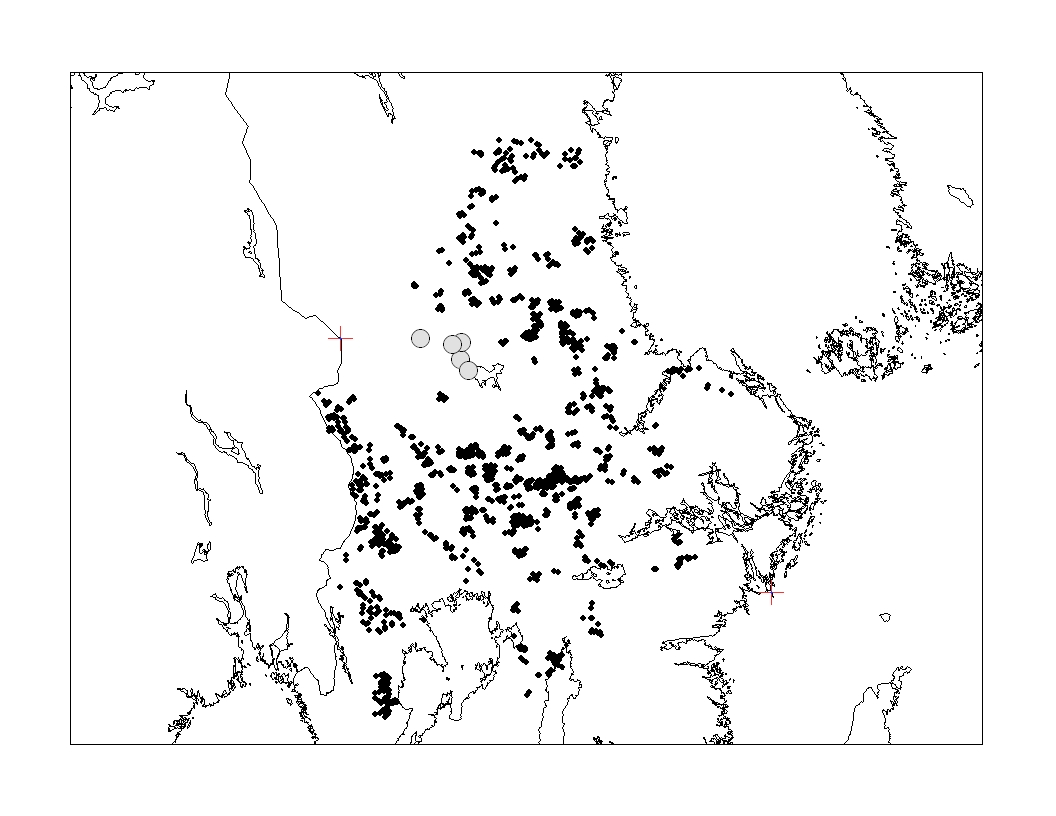
\includegraphics[height=.5\textheight]{figures/20_ForestFinns}
\caption{Distribution of “Forest Finns” (black dots) compared to that of non-delimited uses of definite forms (grey circles). Sources: \citet{Tarkiainen1990}, \citet{Broberg1980}.}
\label{map:16}

\end{figure}

\section{ Reconstructing the grammaticalization path}
\label{sec:3.4}

The extended uses of definite forms that we see in the Peripheral Swedish area represent a kind of development that has not been studied from a typological or diachronic point of view, although, as was noted above, it is not without parallels outside Scandinavia. In historical linguistics, like in evolutionary biology, it is often the case that researchers look in vain for the “missing link”, that is, the crucial intermediate stages in a process of change – instead, the details of the process have to be inferred from what we can observe in the present. This also holds here. From written documentation, we know that the patterns in question go back at least to the 18\textsuperscript{th} and almost certainly to the 17\textsuperscript{th} century, but we can only guess at what happened between the introduction of the suffixed definite article, which probably took place at least half a millennium earlier, and the point in time when the first attestations show up. 

Our guesses need not be totally unqualified, however. Among the uses of the definite forms that are “extended” from the point of view of Central Scandinavian (and for that matter, English), not all are equally exotic – on the contrary, as I have noted above, many if not most languages with definite articles tend to use them more systematically with generic noun phrases than English and Central Scandinavian. We can also observe that the area where we find more generic definites than in the standard languages is larger than that, for example, of the non-delimited uses and the low-referentiality singular count uses. Given these observations, it seems natural to look closer at the possibility that generic uses are the stepping-stone to the latter ones. 

This idea indeed seems to make sense also from the semantic point of view. In fact, genericity has sometimes been used as a collective label for the extended uses: thus, \citet[134]{Hummelstedt1934}, speaks of “allmän eller generell betydelse”,\footnote{ This quotation is difficult to translate since \textit{allmän} and \textit{generell} both mean ‘general’ in Swedish.} \citet[29]{Marklund1976} of “totality meaning” [totalitetsbetydelse] and \citet{BergholmEtAl1999} suggest the term “generic article” as a replacement for Delsing’s “partitive article”. Calling something like \textstyleLinguisticExample{beer} in a sentence such as \textstyleLinguisticExample{He’s drinking beer} “generic” certainly presupposes a rather generous definition of that term, but it has to be admitted that the notion of genericity does not lend itself to an easy delimitation. In the section on generic noun phrases above, I distinguished two basic kinds of generic uses of noun phrases. One of the two basic uses of generic noun phrases discussed in \sectref{sec:3.2.1} was “kind predications”, meaning that something is said about a kind or species rather than about its members, e.g. 

\ea
\gl The northern hairy-nosed wombat is an endangered species. 
\z 

The question that arises is whether it is not possible to say that almost any mention of a species constitutes such a “kind predication”. Indeed, one of the major claims in the influential paper by \citet{Carlson1977} was that “existential” uses of bare nouns in English (as in \textstyleLinguisticExample{There are wolves in the forest}) are really kind-referring. In most contexts, there is in fact no ambiguity between generic and existential readings due to restrictions on the syntactic positions in which these readings can occur. However, there are some seemingly genuine cases of ambiguity, such as \REF{158}, which has one clearly kind-referring reading, which is synonymous to \REF{159}, and one existential, which might occur in a context such as \REF{160}.

\ea
\gl \label{bkm:Ref107049066}John studies cats.  
 \z

\ea 
\gl \label{bkm:Ref107049087}John studies the species Felis catus.
\z 

\ea 
\gl \label{bkm:Ref107049114}John studies cats, because he is not allowed to use humans for his experiments. 
\z 

In a language such as French, the two readings of \REF{158} would be distinguished formally, the generic reading taking a definite article and the existential one taking a partitive article. Consider the following quotation from a theological discussion site:

\ea \label{} 
\langinfo{French}{}{}\\
\gll Peut-on,  par  exemple,  étudier  \textbf{l’} \textbf{ Homme}\\
can-one  for  example  study  \textbf{{\deff} } \textbf{man}\\
\gll sans  étudier  \textbf{des} \textbf{hommes?} \\
without  study.{\inf}  \textbf{P{\art}} \textbf{man.{\pl}} \\
\glt ‘Can one for instance study man without studying human beings?’ (Internet)

\z

These observations notwithstanding, the borderline of genericity is rather fuzzy. I said above that it seems that it is often the construction in which a noun phrase appears that determines whether we understand it as generic or not. But another side of the matter is that one and the same content can often be expressed by alternative constructions, only one of which involves a generic noun phrase. For instance, plain existential statements can be paraphrased as statements involving singular definite generics, e.g.:

\ea
\gl There are not many wombats left.  
 \z

\ea 
\gl The wombat is rare these days.
\z 

\ea 
\gl There are lions in Kenya and Tanzania.
\z 

\ea
\gl The lion is represented in both Kenya and Tanzania. 
\z 

These alternative ways of expressing what is basically the same proposition have parallels in cases such as

\ea
\gl \label{bkm:Ref107116648}I suddenly became dizzy.  
 \z

\ea 
\gl \label{bkm:Ref107116651}A sudden dizziness came upon me.
\z 

where the difference is in whether the state of dizziness is expressed via an adjective or highlighted as an abstract noun \textstyleLinguisticExample{dizziness, }which obtains the role of the subject of the sentence. Semantically, this means that the state is “reified” or “hypostasized”, that is, treated as an abstract object. 

As it turns out, there is considerable cross-linguistic variation in how propositions such as those expressed in \REF{166}{}-\REF{167} are constructed grammatically, and some languages may well choose standard ways of expression that are more similar to \REF{167}. Sympathizers of Whorfianism will see this as evidence of differences in how we structure the world. I am personally somewhat skeptical to such hypotheses, at least as far as fully grammaticalized constructions go. That is, if there is just one standard way of expressing some particular content, more substantial evidence is needed to show that this influences the ways people think. But interesting phenomena are observable when different patterns compete. Consider the following Italian sentence:

\ea \label{} 
\langinfo{Italian}{}{}\\
\gll Papa  beve  \textbf{il} \textbf{caffè} ogni  mattina.\\
father  drink.{\prs}.3{\sg}  \textbf{{\deff}} \textbf{coffee} every  morning\\
\glt ‘Father drinks coffee every morning.’ (Internet)

\z

In English or Swedish, using definite marking on ‘coffee’ to express the corresponding content results in a rather weird interpretation (the natural reaction is “what coffee?”). In Italian, on the other hand, it is the article-less alternative that is felt to be weird: Father drinks (an unspecified, and thus unusual amount of) coffee every morning (Pier Marco Bertinetto, personal communication). Thus, the definite article seems to be induced by the fact that coffee is drunk regularly, in more or less specified quantities. 

Similarly, in the following Sicilian sentence (quoted from \citet[413]{BertinettoEtAl2000}, original source: \citet[231]{Skubic1973-74}, and its translation into Italian, the swordfish is, it seems, focused enough to be worth “reifying” by the use of a definite article:

\ea 
	\ea { 
	\langinfo{Sicilian}{}{}\\
	\gll	 Aju  manciatu  tanti  voti  \textbf{u} \textbf{piscispata,}\\
			have.{\prs}.1{\sg}  eat.PP  many  time.{\pl}  \textbf{{\deff}} \textbf{swordfish}\\
	\gll 	e  m’  ha  fattu  sempri  beni.\\
			and  me.{\dat}  have.\textsc{prs.3sg}  do.PP  always  good\\
	}
	\ex {
	\langinfo{Italian}{}{}\\
	\gll 	Ho  mangiato  tante  volte  \textbf{il} \textbf{pesce} \textbf{spada,}\\
			have.{\prs}.1{\sg}  eat.PP  many  time.{\pl}  \textbf{{\deff}} \textbf{fish} \textbf{sword}\\
	\gll 	e  mi  ha  fatto  sempre  bene.\\
			and  me.{\dat}  have.\textsc{prs.3sg}  do.PP  always  good\\
	\glt 	‘I have eaten swordfish many times, and it has always done me well.’
	}
	\z	 
\z

The competition between different grammatical patterns makes it possible for subtle nuances in interpretation to arise (see for further discussion \citet[128-134]{Dahl2004}). If, on the other hand, the use of the definite article in a similar context becomes obligatory, as in the Peripheral Swedish vernaculars, such nuances are lost. Another point to be made in this connection is that usage is often regulated in specific constructions but the way it is regulated may vary from one language to another. Consider, as an example, complements of verbs like \textstyleLinguisticExample{smell}, as in

\ea
\gl He smells of vodka.  
 \z

%\end{listLFOileveli}

In most Germanic languages, it is simply impossible to use definite marking here, and from this point of view, it may seem more plausible to construe such sentences as talking of a restricted quantity of vodka, rather than as involving a kind predication in the sense of \citet{KrifkaEtAl1995}. Nevertheless, in many Peripheral Swedish varieties as well as in French, the normal construction is with a definite article: 

\ea \label{} 
\ea {
\langinfo{Älvdalen (Os)}{}{}\\
\gll An  lupter  \textbf{brendwineð}\\
he  smell.{\prs}  \textbf{vodka.{\deff}}\\
}
\ex {
\langinfo{French}{}{}\\
\gll Il  sent  \textbf{la} \textbf{vodka}\\
he  smell.{\prs}.3{\sg}  \textbf{{\deff}} \textbf{vodka}\\
\glt ‘He smells of vodka.’
}
\z 
\z

This could be interpreted as evidence that Elfdalian and French construe the predicate ‘smell’ as holding between a perceiver and a kind, and that other languages construe it as holding between a perceiver and an indefinite quantity of something. On the other hand, since there is no evidence for such a cognitive difference, it could be argued that it is equally plausible that languages are indifferent to the distinction between these two possible construals. 

The Romance languages, which on the whole seem more generous than Germanic in allowing definite articles in the fuzzy border area of genericity, exhibit some interesting cross-linguistic patterns of variation. \citet{Zamparelli2002} discusses various examples of what looks like extended uses of definite articles in Italian and other Romance languages. According to him, the following cases “force us to conclude that, in Italian, some definites can … have a purely indefinite meaning”. (The glosses in \REF{173}{}-\REF{178} and \REF{182}{}-\REF{184} are Zamparelli’s. The boldface is mine.)

\ea \label{} 
\langinfo{\label{bkm:Ref172696600}\label{bkm:Ref69030048}Italian}{}{}\\
\gll Ogni  settimana,  il mio  sito web\\
every  week,  my  web\_site\\
\gll viene  attaccato  dagli  hacker.\\
is  attacked  by\_{\deff}.{\pl}  hacker\\
\glt ‘Every week, my web site is attacked by \textbf{the hackers}.’

\z

\ea \label{} 
\langinfo{\label{bkm:Ref69030716}Italian}{}{}\\
\gll Nel  1986  \textbf{i} \textbf{ladri} hanno  svuotato\\
In  1986  \textbf{{\deff}} \textbf{thieves} have  emptied\\
\gll il mio  appartamento.\\
my  apartment.\\
\glt ‘In 1986 the thieves emptied my apartment.’

\z

\ea \label{} 
\langinfo{Italian}{}{}\\
\gll La  casa  è  sporchissima.\\
{\deff}  house  is  filthy.\\
\gll In  cantina  ci  sono  \textbf{i} \textbf{topi}\\
In {\deff}  basement  there  are  \textbf{{\deff}} \textbf{mice}\\
\gll e  sotto  il  lavello  vivono  \textbf{gli} \textbf{scarafaggi.}\\
and  under  {\deff}  sink  live  \textbf{{\deff}} \textbf{cockroaches}\\
\glt ‘The house is filthy. In the basement there are the mice and under the sink live the cockroaches.’  

\z

\ea \label{} 
\langinfo{Italian}{}{}\\
\gll Che  fai  per  mestiere?  Fotografo  \textbf{gli} \textbf{  uccelli.}\\
What do you  do  for  {\indf} living?  I photograph  \textbf{{\deff}} \textbf{bird.{\pl}}\\
\glt ‘What do you do for a living? I photograph the birds.’

\z

\ea \label{} 
\langinfo{Italian}{}{}\\
\gll Con  questi  disturbi  ho  dovuto\\
with  this  condition  I  had to\\
\gll smettere  di  bere  \textbf{il} \textbf{caffè.} \\
stop  to  drink  \textbf{{\deff}} \textbf{coffee.}\\
\gll \textbf{Il} \textbf{tè} invece  mi facilita  la digestione.\\
\textbf{{\deff}} \textbf{tea} instead  helps  the digestion.\\
\glt ‘With this condition I had to stop drinking the coffee. The tea instead helps my digestion.’

\z

\ea \label{} 
\langinfo{\label{bkm:Ref172696628}Italian}{}{}\\
	\gll Gianni  è  così  pallido  che  sembra\\
Gianni  is  so  pale  that  it seems\\
\gll abbia  visto  \textbf{i} \textbf{fantasmi.}   \\
he has  seen  \textbf{{\deff}} \textbf{ghosts}   \\
\glt ‘Gianni is so pale that it seems he has seen the ghosts.’

\z

Zamparelli’s examples have in common that it is not natural to preserve the definite article when translating into English. They differ from each other in various ways, however. Consider, to start with, \REF{173}. It is not generic in the sense that it is a general statement about hackers. Rather, what it says is that every week, some hackers visit my site. Whether it is the same persons every week or not is not said, and probably the speaker does not know. What could be argued here is that in \REF{173}, the hackers who visit my site are seen as representatives of the world-wide community of hackers, as it were. Similarly, the mice in the basement in \REF{174} could be thought of as representing the mouse species in general. This would make \REF{173} and \REF{174} a bit similar to a sentence such as the following: 

\ea
	\gl \label{bkm:Ref69031158}The Americans have visited the moon.  
\z

\ea 
\gl \label{bkm:Ref77501116}Swedish
\z
 
\ea\label{}
\gll \textbf{Räven} har  varit  i  hönshuset  igen.\\
\textbf{fox.{\deff}} have.{\prs}  be.{\supp}  in  hen-house.{\deff}  again\\
\glt ‘The fox has been in the hen-house again.’

\z

There are clear differences here though. In English, the conditions for using the definite article in a “representative” sense are stricter than in Italian. It appears that the reason one can say something like \REF{179} is that the American visitors to the moon were representatives of the American nation not only in some extended or metaphorical sense but also quite concretely, since they acted on behalf of the US government. When it becomes possible to go to the moon as a tourist, it clearly will not be sufficient for me and some of my friends to go there for \REF{181} to be true.

\ea
\gl \label{bkm:Ref94431191}The Swedes have visited the moon.  
 \z

	 \REF{180} is different from Zamparelli’s example in that the noun phrase is in the singular. Zamparelli notes that if \textstyleLinguisticExample{il topo} ‘the mouse’ is substituted for \textstyleLinguisticExample{i topi }in \REF{174}\textstyleLinguisticExample{, }the interpretation has to be specific. A prerequisite for the use of a singular in \REF{180} is that foxes tend to operate one by one, in such a way that we can think of the fox that visited the hen-house last night as a representative of the fox species. 

Zamparelli notes that the three Romance languages Italian, Spanish and French differ in how readily they accept definite noun phrases in contexts of this kind. Thus, in the French translation of \REF{174}, only partitive articles are possible. In Spanish, definite articles are possible, but not with the existential verb \textstyleLinguisticExample{hay} ‘there is’, only with verbs such as \textstyleLinguisticExample{estar} ‘be’ and \textstyleLinguisticExample{vivir} ‘live’:

\ea \label{} 
\langinfo{\label{bkm:Ref172696738}French}{}{}\\
\gll Dans  la  cave,  il  y  a  \textbf{?les} \textbf{/} \textbf{des} \textbf{souris,}\\
in  {\deff}  basement  it  there  have  \textbf{{\deff}}  \textbf{P{\art}{\art}} \textbf{mouse.{\pl}}\\
\gll et  dans  l’  évier  vivent  ?les  /  des  cafards.\\
and  in  {\deff}  sink  live.{\prs}.3{\pl}  {\deff}    P{\art}{\art}  cockroaches\\
\glt ‘In the basement there are the mice and under the sink live the cockroaches.’ 

\z

\ea \label{} 
\langinfo{Spanish}{}{}\\
\gll En  el  sótano  hay  \textbf{(*los)} \textbf{  ratones,}\\
In  {\deff}  basement  exist  \textbf{({\deff})} \textbf{mice,}\\
\gll y  bajo  la  fregadera  hay  \textbf{(*las)} \textbf{cucarachas.}\\
and  under  {\deff}  fridge  exist  \textbf{({\deff})} \textbf{cockroaches}\\
\glt ‘In the basement there are mice and under the fridge there are cockroaches.’  

\z

\ea \label{} 
\langinfo{\label{bkm:Ref172696740}Spanish}{}{}\\
\gll En  el  sótano  están  \textbf{*(los)} \textbf{  ratones,}\\
In  {\deff}  basement  are  \textbf{({\deff})} \textbf{mice}\\
\gll y  bajo  la  fregadera  vivon  \textbf{*(las)} \textbf{cucarachas.}\\
and  under  {\deff}  fridge  live  \textbf{({\deff})} \textbf{cockroaches}\\
\glt ‘ In the basement are mice and under the fridge live cockroaches.’  

\z

What we see here, then, is a cline of acceptability for definite noun phrases in uses that can be seen as non-delimited, with French being most restrictive and Italian being most liberal. This then suggests a way by which definite noun phrases may expand their domain of use into the indefinite territory with the situation in the Peripheral Swedish vernaculars or Moroccan Arabic (see \sectref{sec:3.2.3.2} above) as the eventual result. In the absence of historical data, it is of course impossible to verify whether the route has been exactly the same, but given the other circumstances mentioned in the beginning of this section, generic uses must be regarded as a highly probable diachronic source for the extended uses of definite forms. 

For singular count nouns, there are also non-generic uses of definite-marked noun phrases than generic ones that could serve as bridging cases. Consider the following sentences in English:

\ea
\gl \label{bkm:Ref123724733}Did you bring \textbf{the knife}\\?
\z 

\ea 
\gl \label{bkm:Ref123724734}Did you bring \textbf{a knif}e\\?
\z 

In many situations, both \REF{185} and \REF{186} would be acceptable. (Imagine, for instance, a picnic.) It is often rather irrelevant if a specific knife is held in mind or not. In Swedish, one could use any of the following three variants:

\ea \label{} 
\langinfo{Swedish}{}{}\\
\gll Tog  du  med  dig  \textbf{kniven/en kniv/kniv?}\\
take.{\pst}  you  with  you  \textbf{knife.{\deff}/{\indf} knife/knife}\\
\glt ‘Did you bring a knife?’

\z

It thus seems plausible that the fluidity of the use of articles here could set the scene for the expansion of the definite forms. In fact, this fluidity sometimes makes it difficult to evaluate uses of definite markings in written sources. Consider the following excerpt from a recording of a speaker born in 1881 and coming from Hållnäs, one of the linguistically most conservative parishes in Uppland:

\ea \label{} 
\langinfo{\label{bkm:Ref123725093}Hållnäs (Up)}{}{}\\
{}[The speaker is describing how sheep were collected from their summer-pasture in the autumn.]\\
\gll 	Å  den  såm  hadde  nô  förstånd  då  se  feck\\
		and  he  who  have.{\pst}  some  sense  then  see.{\imp}  get.{\pst}\\
\gll 	han  ju  ha  \textbf{bröy-sättjin,} helle  \textbf{bröy-kôrjin,} å\\
		he  {\prag}  have.{\inf}  \textbf{bread-sack.{\deff}} or  \textbf{bread-basket.{\deff}} and\\
\gll 	le{\textasciigrave}t  åpp  en  ta´ckâ  såm  fåLd  etter.\\
		search.{\inf}  up  {\indf}  ewe  who  follow.{\pst}  after\\
\glt  ‘And he who had some sense got to have the bread sack, or the bread basket, to find a ewe who was lagging behind.’ (\citet[33]{KällskogEtAl1993})

\z

Speakers of standard Swedish do not react to the use of definite forms here, but if \REF{188} had occurred in a Peripheral Swedish area vernacular, it could relatively easily be seen as parallel to the examples discussed in \sectref{sec:3.2.5}.

Many of the extended uses of definite forms seem rather eccentric from the point of view of standard definitions of definiteness. As was mentioned above, it is a general characteristic of advanced stages of the evolution of definite articles that the semantic element of definiteness is weakened or gets lost entirely, as when articles develop into general affixes on nouns. Such a loss of the semantic essence of a morpheme may appear paradoxical, in that the motivation for having a definite article in the first place ought to be to express definiteness. In the words of \citet[91]{Hawkins2004}, “why should the definite article be recruited for more and more NPs in performance and grammar and gradually jettison the semantic-pragmatic conditions of its deictic source?”  Hawkins suggests that the answer has to be found in the processing of grammar: the functions of definite articles that become dominant at later stages of its evolution are to “construct a (case-marked) NP” and to “attach specified categories to the (case-marked) NP that it constructs”. It is not clear from Hawkins’ text if “construct” means anything but “unambiguously signal”, but the consequence is in any case that the function of a definite article is syntactic rather than semantic. Hawkins notes (quoting \citet[64]{Lyons1999}) that the cross-linguistic tendency for definite articles to occur early in noun phrases can be explained through the necessity to signal the NP-hood of an expression early on. Notice that the principle “Signal NP-hood as early as possible” would have much of the same effect as the principle “The D-position must be filled” suggested by Holmberg \& Sandström. However, Hawkins’ principle makes most sense in complex NP’s, where an article preposed to or cliticized to the first word would function much as a labeled left bracket. It is less clear what the point of having a definite article on a bare noun would be. Perhaps we should see the function of definite articles whose use is extended beyond what is warranted by semantic definiteness as enhancing the general level of redundancy in grammar and thus making the transmission of the message safer (see \citet[9-11]{Dahl2004}). It should be added that any theory which attributes too essential a role to definite suffixes in varieties like the Peripheral Swedish ones will have problems explaining the tendency in the same varieties towards extensive neutralization of the distinction between definite and indefinite forms. 


 \newcommand{\textcyrillic}{}
\chapter{Attributive constructions}
\section{Introduction}
\label{bkm:Ref262028996}

One area of grammar where Scandinavian languages show some well-known peculiarities is in the expression of definite noun phrases which contain preposed attributes. In all varieties of Central Scandinavian, a preposed definite article is employed in such noun phrases; however, whereas this article in Danish has a complementary distribution to the ordinary suffixed article, as illustrated by \textstyleLinguisticExample{det store hus} ‘the big house’ (as opposed to \textstyleLinguisticExample{huset} ‘the house’), Swedish (and also normally Norwegian) uses both articles, as in \textstyleLinguisticExample{det stora huset} ‘the big house’. However, in northern Scandinavia, there is a radically different way of combining an adjective and a noun: the normal translation of ‘the big house’ would be something like \textstyleLinguisticExample{stor-hus-et} ‘big-house-DEF’, where the adjective is incorporated into the noun and there is no preposed article. In this chapter, I shall discuss this construction and a number of additional variations on the general theme that contribute to a quite variegated picture. However, one challenge in doing so is the tight interaction of several different parameters with different histories and geographical distribution. Another problem is the low frequency of adjectival modifiers in definite noun phrases (noted by \citet{Thompson1988}). In the corpus \textit{Samtal i Göteborg }(\citet{Löfström1988}), comprising half a million words of spoken Swedish – corresponding to 1250 printed pages, there were only 253 examples of the pattern

\ea 
\gl den/det/dom Adj-e/a N-DEF
\z 

that is, the standard form of such NPs in Swedish. (Comparatives and superlatives were excluded from this count.) This is equivalent to about once in ten minutes of conversation, or once in five printed pages. In addition, it turns out that a few adjectival lexemes had a rather dominant place among those examples: about 40 per cent consisted of tokens of the four adjectives \textstyleLinguisticExample{stor }‘big’, \textstyleLinguisticExample{liten} ‘small’, \textstyleLinguisticExample{gammal} ‘old’, \textstyleLinguisticExample{ny} ‘new’. It is probably no accident that these items are among the cross-linguistically prototypical adjectives in the sense that they show up in practically every language that has a separate class of adjectives.\footnote{\label{fnt:ftn36} According to \citet{Dixon1977}, the adjectives that occur most frequently across languages are ‘large’, ‘small’, ‘long’, ‘short’, ‘new’, ‘old’, ‘good’, ‘bad’, ‘black’, ‘white’.} In written dialect texts, which are either direct renderings of spoken language or else tend to be close to spoken language in form, the corresponding patterns also show up very sparingly.

\section{Definite marking in attributive constructions: The typological perspective}

As it turns out, it is quite common cross-linguistically for attributive constructions to show some peculiarities with respect to definiteness marking. Thus, we find languages in which definiteness is only marked when a noun phrase contains a modifier, as in Latvian which has suffixed definite articles on adjectives, although it does not otherwise use definite marking, as illustrated by the following examples. 

\ea\label{}
\langinfo{Latvian}{}{}
\ea {
\gll liel-a  m\=aja\\
big-F.NOM.SG  house\\
\glt ‘a big house’
}

\ex {
\gll liel-\=a  m\=aja\\
big-F.NOM.SG.DEF  house\\
\glt ‘the big house’
}
\z 
\z 

In another pattern, an article that usually sits on the noun shows up on the adjective in an attributive construction, as exemplified by Amharic:

\ea\label{}
\langinfo{Amharic }{}{}
\ea {
\gll bet-u\\
house-DEF\\
\glt ‘the house’
}

\ex {
\gll t\textcyrillic{?ll?q-}u  bet\\
big-DEF  house\\
\glt ‘the big house’
}
\z 
\z 

Finally, the phenomenon of double articles is by no means restricted to Scandinavian. Consider, for example, Standard Arabic, in which the noun and the adjective each take the identical article \textstyleLinguisticExample{al}:

\ea\label{}
\langinfo{Standard Arabic}{}{}
\ea {
\gll al\textbf{{}-}bayt\\
DEF-house\\
\glt ‘the house’
}

\ex {
\gll al\textbf{{}-}bayt  al\textbf{{}-}kabir\\
DEF-house  DEF-big\\
\glt ‘the big house’
}
\z 
\z 

From Germanic languages, we can mention Yiddish, where double articles are optional and more likely to appear when the adjective is postposed (\citet[342-347]{Plank2003})

\ea\label{}
\langinfo{Yiddish}{}{}
\ea {
\gll di  grine  oygn\\
DEF  green.PL  eye.PL\\
\glt ‘the green eyes’
}

\ex {
\gll di  oygn  di   grine\\
DEF  eye.PL  DEF  green.PL\\
\glt ‘the green eyes’
}
\z 
\z 

Even closer to home, in Old Icelandic, we find cases where two preposed definite articles are combined with a suffixed definite article on the noun. This triple marking is certainly a challenge for any theory that supposes that each morpheme fills a separate slot in the underlying structure. The following example is from the saga of Gísli Súrsson. The protagonist is having recurrent dreams where two dream-women, one good and one bad, appear: 

\ea\label{}
\langinfo{Old Icelandic}{}{}
\gll Hann  segir,  att  nú  kom  at  honum\\
he  say.PRS   that  now  come.PRS  to  he.DAT\\
\gll \textbf{draumkona}\textbf{{}-n}\textbf{  sú} \textbf{hin} \textbf{verri…}\\
\bfseries dreamwoman-DEF  DEF  DEF  worse\\
\glt ‘[Reporting Gísli’s answer to a question about his dreams:] He says that now came to him the evil dream-woman…’ (Gísla saga Súrssonar 33)
\z

%\begin{styleTextkrper}
 See \citet{Dahl2003} for further examples and discussion.

%\end{styleTextkrper}

\section{Survey of attributive definite NP constructions}
\label{bkm:Ref224464037}\subsection{The deprecated standard: the Scandinavian preposed article}
\label{bkm:Ref154983973}\label{bkm:Ref154988501}

Like the suffixed article, the preposed definite article in Scandinavian goes back to medieval times, and the earliest attestations are from texts from Iceland and Norway where the pronouns \textstyleLinguisticExample{hinn }and\textstyleLinguisticExample{ enn} were used early on in this function. In Early Written Medieval Swedish, as described by \citet{Larm1936}, there was competition between several different ways of expressing definite NPs with preposed attributes. Most often, only one article was used, but it could be either a preposed or a suffixed one, thus either \textit{þæn gamli man} or \textit{gamli mannin}. The preposed article – in the beginning sometimes \textstyleLinguisticExample{hinn} but more frequently \textstyleLinguisticExample{þæn}, another originally demonstrative pronoun \textstyleLinguisticExample{ – }was more common in poetic language and the suffixed one most frequent in prose, although even there the preposed alternative was preferred – the overall ratio between the two articles was 10:1. The alternative with double articles seems to have become a serious contestant only later. The distribution of the two articles over genres suggests that the preponderance of the preposed article in poetry “essentially depends on foreign influence” (\citet[68]{Larm1936}).\footnote{ “…att den rika frekvensen av typen \textit{þæn gamli man} i poesien till väsentlig grad beror på främmande inverkan.”} According to Larm, there is a difference in deictic force between the two alternatives as used in prose, in that \textstyleLinguisticExample{þæn} tends to be used in contexts that are more similar to those of “normal” demonstratives. Larm thus concludes that contrary to what earlier researchers such as Falk-Torp and Nygaard had proposed, the preposed article \textstyleLinguisticExample{þæn} cannot be older than the suffixed one\footnote{ “\textit{Þæn }såsom artikel kan ej vara äldre än suff. artikel.” } (\citet[64]{Larm1936}).

It is consonant with this view to assume that the preposed article arrived later in the Swedish dialect area than the suffixed article. In fact, as we shall now see, the use of the preposed article is still more restricted in Standard Swedish than in Standard Danish. 

In \citet{Dahl2003}, I discuss in some detail two classes of cases where the preposed article does not show up, viz. what I call \textbf{selectors} and \textbf{name-like uses}. I use “selectors” as a cover term for three categories that are usually treated separately in Swedish grammars (all examples are Swedish):

\begin{enumerate}
%\begin{styleMyNumberedList}
\item a subset of what \citet[435]{TelemanEtAl1999}) call “relational pronouns”: “ordinative pronouns”, e.g. \textit{först(a}) ‘first’, \textit{sist(a)} ‘last’, \textit{nästa} ‘next’, \textit{förra }‘previous’, “perspectival pronouns”, e.g. \textit{höger/högra }‘right (hand)’, \textit{vänster/vänstra} ‘left (hand)’, \textit{norra} ‘north’ etc., \textit{övre} ‘upper’ etc., and \textit{ena} ‘one (of)’ 

%\end{styleMyNumberedList}

%\begin{styleMyNumberedList}
\item ordinal numerals

%\end{styleMyNumberedList}

\item superlatives

%\begin{styleMyNumberedList}

%\end{styleMyNumberedList}

%\end{listLFOvileveli}

\end{enumerate}

All these categories share a common semantics – they are all “inherently definite” in that the noun phrases they are used in normally have definite reference by virtue of their meaning. The term “selector” is motivated by the fact that they pick out a member or a subset of a specific superset by the help of some relation between that member or subset and the set as a whole. In other words, if I say e.g. \textstyleLinguisticExample{yngste sonen} ‘the youngest son’, I pick out one of the sons by relating him in age to the others: he may not at all be young if considered in isolation. 

All three types of selectors show up with nouns in the definite form without a preposed article, e.g. \textstyleLinguisticExample{norra delen} ‘the northern part’, \textstyleLinguisticExample{första gången} ‘the first time’, \textstyleLinguisticExample{äldsta dottern} ‘the eldest daughter’. In addition, the first type (“relational pronouns”) also occurs without any definite marking at all, in spite of the noun phrases in question having definite reference: \textstyleLinguisticExample{nästa sommar} ‘next summer’, \textstyleLinguisticExample{höger hand} ‘the right hand’. It appears that the interpretation of the unmarked cases tends to involve the deictic center. Often, the corresponding phrases in English are also articleless, and the pattern also shows up in the other Central Scandinavian languages. Selectors with a suffixed but no prefixed article are only found in Swedish and to some extent in Norwegian Bokmål but not at all in Danish. As I showed in \citet{Dahl2003}, they also appear to be considerably less popular in the vernaculars from the Southern and Göta dialect areas within the Swedish dialect area, judging from the Cat Corpus material. Compare the following sentence in Swedish and the text from Träslövsläge in Halland (similar examples are also found in texts from Skåne, Bohuslän, and Västergötland):

\ea\label{}
\ea { 
\langinfo{Swedish}{}{}
\gll \textbf{Äldsta} \textbf{pojken} hade  rest  till  Amerika.\\
\textbf{old.SUPERL.WK} \textbf{boy.DEF} have.PST  go.SUP  to  America\\
}
\ex {
\langinfo{Träslövsläge (Hl)}{}{}

\gll \textbf{Den}\textbf{  gamlaste}\textbf{  päjken} hade  fåt  te  Amerka.\\
\textbf{DEF} \textbf{old.SUPERL.WK} \textbf{boy.DEF} have.PST  travel.SUP  to  America\\
\glt ‘The eldest boy (i.e. Granny’s son) had gone to America.’ (Cat Corpus)
}
\z
\z 

A similar situation shows up with “name-like uses” of definite articles. This includes, on one hand, lexicalizations of noun phrases containing an adjectival modifier and a head noun as in \textstyleLinguisticExample{Vita huset} ‘the White House’, and on the other, expressions that have not yet reached the status of lexical items but which are used to refer to well-known objects, typically chosen out of a small set. For instance, if you own two houses next to each other but of different size, it is very natural to call them \textstyleLinguisticExample{stora huset} ‘the big house’ and \textstyleLinguisticExample{lilla huset} ‘the little house’, even before these denominations have become so “entrenched” that capital letters would be used in writing. We can see that such cases are fairly similar to the cases with selectors discussed above. Name-like uses are treated quite differently in the Central Scandinavian languages. In Danish, we find either (i) the usual pattern with a preposed article and no definite marking on the noun (\textstyleLinguisticExample{Det Hvide Hus} ‘the White House’), (ii) no definite marking whatsoever (\textstyleLinguisticExample{Nordisk Råd} ‘the Nordic Council’) or (iii) definite marking only on the adjective, i.e. by choosing the weak form (\textstyleLinguisticExample{Store Bælt} ‘the Big Belt, i.e. the sound between the islands of Sjælland and Fyn’). In no case do we find a definite form of the noun, however. All three Danish patterns are also found in Swedish, more or less marginally. The first pattern is found in archaic expressions such as (i) \textstyleLinguisticExample{den helige Ande} ‘the Holy Ghost’ and the second occasionally in names such as  \textstyleLinguisticExample{Svensk Uppslagsbok} ‘The Swedish Encyclopedia’. The third pattern is represented in toponyms such as \textit{Store Mosse} ‘Large Peatbog’ over most of the South Swedish and Göta dialect areas. As for Norwegian, Bokmål, which in other cases has double articles, goes with Danish here, but Nynorsk stands out by using double articles even in these contexts (e.g. \textstyleLinguisticExample{Det Kvite Huset} ‘the White House’). 

Generalizing from these patterns, it can be said that all Central Scandinavian languages (in which I do not count Nynorsk) show tendencies to have less definiteness marking with selectors and name-like uses than in other cases of definite noun phrases with preposed modifiers. In general, there tends to be less marking of noun phrases whose definiteness is in one way or the other “inherent”; in diachronic developments, they tend to be the last ones to receive marking. With respect to the preposed article, it appears fairly clear that it is generally stronger in Denmark than in the other Scandinavian countries, especially Sweden. If we consider also the non-standard varieties, we can see that there is in fact a cline going from south-west to north-east, with the preposed article becoming gradually weaker as we move along it. In south-western Jutland, the preposed article is used universally and the suffixed article does not exist. Southern Swedish vernaculars are less restrictive than Standard Swedish in the use of the preposed article, that is, they are more like Standard Danish. On the other hand, in the Peripheral Swedish area, in particular the more conservative parts, preposed definite articles of the Central Scandinavian type are quite restricted and are possibly largely ascribable to influence from Swedish. 

\subsection{The celebrated competitor: Adjective incorporation}

Adjective incorporation is one of the more well-known peculiarities of the vernaculars of the Peripheral Swedish area, although the term itself has come into use only fairly recently (probably first in \citet{SandströmEtAl}); traditionally, the phenomenon has been seen as “compounding”. Now, compounds consisting of an adjective and a noun are quite common in all varieties of Scandinavian, as in other Germanic languages. It is often noted in the literature that adjective-noun compounds are found more often in Northern Swedish vernaculars than in Central Scandinavian, but it is important to see that there is also a semantic difference, and that adjective-noun combinations found in Northern Scandinavia tend to be used in ways that are not normally possible with adjective-noun compounds. Consider, for example, the following Elfdalian sentence:

\ea\label{}
\langinfo{Älvdalen (Os)}{}{}
\gll In[1EB?]  guäve;  add\\
on  floor.DEF.DAT  have.PST\\
\gll an  laggt  ien  filt  briewið  \textbf{wåtjakku.}\\
he  lay.SUP  INDF  blanket  next\_to  \textbf{wet\_jacket.DEF.ACC}\\
\glt  ‘On the floor, he had put a blanket next to the wet jacket.’ [S9]
\z

In Swedish or English, a compound like \textstyleLinguisticExample{våtjacka} or \textstyleLinguisticExample{wet-jacket} could only be used for a special kind of jacket that is permanently wet, or perhaps more plausibly, for a jacket intended for use in wet conditions. Similarly, \textstyleLinguisticExample{wetland} or the synonymous Swedish \textstyleLinguisticExample{våtmark} denote an area characterized by being permanently water-soaked. By contrast, the Elfdalian expression refers to a jacket that is in a temporary state of wetness. In other words, it functions just like the English phrase \textstyleLinguisticExample{the wet jacket}. One way of thinking of the distinction is in terms of the number of concepts involved. In the case of ordinary compounds, such as \textstyleLinguisticExample{wetland}, we are dealing with a unitary concept, more or less permanently established. In the case of the phrase ‘the wet jacket’, we have a more or less accidental combination of the two concepts ‘wet’ and ‘jacket’. It is the possibility of using the Elfdalian expression in such an “occasional” way that motivates using the term “incorporation” rather than “compounding”. 

In some cases, we get quite distinct readings of one and the same adjective-noun combination. Thus, the phrase \textstyleLinguisticExample{the new car} might mean either ‘the car I just bought (in contrast to the one I had before)’ or ‘the recently fabricated car’. In Swedish, there is a compound \textstyleLinguisticExample{nybil} which has only the second reading in the standard language. In the vernaculars where adjective incorporation is possible, this tends to be true of the indefinite form, but the definite form \textstyleLinguisticExample{nybiln }will also have the reading of referring to a new car that is contrasted to a car I had before (\citet[91]{SandströmEtAl2003}). In fact, the presence of such readings of combinations with an adjective like ‘new’ is a relatively certain indicator that we are dealing with something more than “ordinary compounding”.

In generative theory, where a sharp distinction between “lexicon” and “syntax” is normally postulated, it is natural to assume, as \citet{SandströmEtAl} do, that compounding belongs in the lexicon and incorporation in the syntax. However, the distinction between incorporation and compounding is a tricky one and should probably rather be seen as a continuum, as I argue in \citet[Ch.10]{Dahl2004} where I discuss incorporating patterns in general. In fact, this distinction between incorporation and compounding often becomes blurred. In a relatively large number of cases, it is not possible to determine whether we are dealing with a unitary concept or not. Many of the examples in the literature which are quoted as examples of the tendency to use adjective-noun compounds instead of ordinary attributive constructions are indeterminate in this way, making it hard to pinpoint the geographical distribution of the phenomenon. I think it is fairly clear that in addition to the use of clear cases of adjective incorporation in the Peripheral Swedish area, there is also a general predilection for adjective-noun compounding which raises the general frequency of such compounds relative to other Germanic languages. This means that one-word adjective-noun combinations are more common not only in definite but also in indefinite NPs. I shall return to the issue of indefinite NPs after an excursion into language typology.

\textbf{Typological considerations.} In the general linguistic literature, adjective incorporation is a somewhat neglected phenomenon, at least in comparison to noun incorporation, that is, the process by which a noun stem is incorporated into the verb of a sentence. Still, in some languages, adjective incorporation is the normal way of adding an attributive adjective to a noun, either generally, as in Lakota, a Siouan language (\citet{BoasEtAl}), or under certain conditions, as in Chukchi (\citet[526]{Muravyova1998}), a Chukchi-Kamchatkan language in which attributive adjectives are obligatorily incorporated when the head noun is in a non-absolutive case.

There are also many examples of attributive constructions which cannot be regarded as full-fledged incorporation but which are still “tighter” than normal adjective-noun constructions. As a general tendency, these tighter constructions seem to be favoured by a low prominence of the adjective and are often restricted to a few adjectives, usually “prototypical” ones, such as ‘big’, ‘small’, ‘old’, ‘new’, ‘good’, ‘bad’, i.e. the ones that show up in languages in which adjectives are a closed class with a small number of members (see fn. \REF{fnt:ftn36}). It has been observed (\citet{CroftEtAl}) that preposed modifiers are more tightly integrated into a noun phrase than postposed ones, for instance by lacking normal grammatical markings. This can be illustrated by pairs such as Spanish \textstyleLinguisticExample{el gran libro }‘the great book’ – \textstyleLinguisticExample{el libro grande} ‘the big book’. Italian, the Celtic languages, Persian, Komi and Southern Ute also exhibit this kind of phenomenon. 

For a more detailed survey of adjective incorporation from a typological point of view, see \citet[225-236]{Dahl2004}.

\textbf{Indefinite adjective-noun combinations}. I claimed above that there is a general predilection in Peripheral Swedish vernaculars for one-word adjective-noun combinations, not only in definite NPs (see also \citet[44, Fn 19]{Delsing2003a}). Many references in the literature to the phenomenon do not distinguish indefinite and definite noun phrases and the examples given are often indefinite ones (for a case in point, consider the examples from \citet{Hedblom1978} quoted below in \sectref{sec:4.4}). 

The question, then, is what is the status of these indefinite adjective-noun combinations. Acknowledging that “Northern Swedish”, i.e. primarily Westrobothnian, has a “relatively productive formation of adjective-noun compounds”, \citet[91]{SandströmEtAl2003} claim that there are two major differences between (i) compounds as used in indefinite noun phrases and (ii) what they see as true cases of adjective incorporation in definite noun phrases.

The first difference according to Sandström \& Holmberg is that indefinite adjective-noun compounds are restricted to monosyllabic adjective stems. Thus, they say, examples such as *\textstyleLinguisticExample{en vackerkweinn }‘a beautiful woman’ and *\textstyleLinguisticExample{en duktipajk }‘an able boy’ are impossible. However, \citet[47]{BergholmEtAl1999} provide counterexamples from Burträsk (NVb) and Sorsele (SVb) such as \textstyleLinguisticExample{magersteint} ‘lean girl’ and \textstyleLinguisticExample{vackerkwinn} ‘beautiful woman’. In the Cat Corpus, we find \textstyleLinguisticExample{magerstackar} ‘lean poor thing’ in the text from from Sävar (SVb) and the following example with the bisyllabic stem \textstyleLinguisticExample{gåmmel-} ‘old’ from Northern Westrobothnian:

\ea\label{}
\langinfo{\textit{Skelletmål} (NVb)}{}{}
\gll …hä  ha  vorte  möittje  bättär\\
it  have.PRSs  become.SUP  much  better\\
\gll seda  I  bört  å  håå\\
since  I  begin.PST  INFM  have.INF\\
\gll \textbf{ä}\textbf{  gåmmel-kattskinn} där  om  netträn.\\
\textbf{INDF} \textbf{old-catskin} there  at   night.DEF.PL\\
\glt ‘…it [my back] has become much better since I began to put an old cat skin there at night.’ (Cat Corpus) 
\z

From the Ovansiljan area we can cite \citet[52]{Levander1909} examples \textstyleLinguisticExample{klakkug-dsieter} ‘horn-less goats’ and \textstyleLinguisticExample{digger-frunt} ‘fat woman’ (both Elfdalian), and from the Cat Corpus, \textstyleLinguisticExample{nog blickna-blad} (Älvdalen) ‘some withered leaves’ and \textstyleLinguisticExample{no blitseblar }(Mora, same meaning). A more extreme example is \textstyleLinguisticExample{nykuäkaðpärur}\textbf{ }‘newly boiled potatoes’ (Elfdalian, \citet[201]{Åkerberg2012}). (Cf. also the examples from Nederkalix quoted below.) Thus, it is possible that the restriction holds for some variety, but definitely not generally for the Peripheral Swedish area and not even for Westrobothnian. 

The other difference between definite and indefinite adjective-noun combinations cited by Holmberg \& Sandström is semantic and thus potentially of a more fundamental nature. According to them, indefinite adjective-noun compounds do not have all the readings of the definite incorporated ones; thus, \REF{198} can only mean that the person in question has bought a newly made car, not one that is “new for him”:

\ea\label{}
\langinfo{\label{bkm:Ref154565993}Westrobothnian}{}{}
\gll Han  ha  tjöfft  sä  \textbf{n}\textbf{  nybil.}\\
he  have.PRS  buy.SUP  REFL  \textbf{INDF} \textbf{new.car}\\
\glt ‘He’s bought himself a new car.’
\z

Yet, it does appear that indefinite adjective-noun combinations in Peripheral Swedish have uses that would not be expected of “normal” compounds, in particular in cases where the adjective signals an accidental or “occasional” property of the referent rather than forms a designation of a “unitary concept” together with the noun. Consider the following example from Elfdalian (\citet[142]{Levander1909}):

\ea\label{}
\langinfo{Älvdalen (Os)}{}{}
\gll Gok  etter  \textbf{ien} \textbf{sturwiðåbörd!}\\
go.IMP  after  \textbf{one.F.DAT} \textbf{big.firewood.load}\\
\glt ‘Go and get a big load of firewood!’ 
\z

\citet[141]{Rutberg1924} gives a number of examples from Nederkalix (Kx), some of which have a definite “occasional” ring: \textstyleLinguisticExample{in litn artibåt }‘a nice little boat’, \textstyleLinguisticExample{i vokkert röbat} ‘a beautiful red band’, \textstyleLinguisticExample{småswartskou} ‘small black boots’, \textstyleLinguisticExample{i vokke-li$\lambda $-bån} ‘a beautiful little child’, \textstyleLinguisticExample{in lil-fåti-ståkkar} ‘a poor little thing’, \textstyleLinguisticExample{i sta-skallat-kou} ‘a big hornless cow’.

In fact, \citet[51]{Levander1909} says explicitly that Swedish indefinite adjective-noun combinations “usually” correspond to compounds in Elfdalian, and in his general treatment of Dalecarlian (\citet[142]{Levander1928}), he echoes this statement by saying that “at least in Älvdalen” compounding is “incomparably much more frequent” than the syntactic construction.\footnote{ “Dylik sammansättning av adj. och subst. är åtminstone i Älvd. ojämförligt mycket vanligare än de båda ordens uppträdande bredvid varandra som skilda ord.”} It is possible, as \citet[44, Fn 19]{Delsing2003a} suggests, that the tendency is stronger in Dalecarlian than in Upper Norrland, or in parts of it, if we consider the examples from Nederkalix above. \citet[98]{Dahlstedt1962} says about Vilhelmina (SVb) that “it does not seem to offend linguistic intuitions to use relatively occasional word combinations as compounds … but this type of formation is not the usual one.” His examples are \textstyleLinguisticExample{n gammbjärkbränne} ‘an old forest clearing, overgrown by birch’ and \textstyleLinguisticExample{n tôkken gammstyggôbb }‘such an ugly old man’ (at least the first one seems like a possible lexicalization to me, though). 

I think these circumstances give support to the idea that there is no clear borderline between compounding and incorporation and also that indefinite one-word adjective-noun combinations can have incorporation-like properties in Peripheral Swedish vernaculars. In any case, it seems unlikely that the one-word combinations we find in indefinite and definite NPs are diachronically wholly separate from each other.

\textbf{Combinations with other determiners. }In the simplest possible case of adjectival modifiers, there are no other elements in the NP than the adjective and the head noun. A definite noun phrase may also contain other elements, however, notably demonstratives (which, as we shall see in \sectref{sec:4.3.4}, are often used much like preposed definite articles). There is considerable variation as to the extent to which adjectives are incorporated in such contexts, which partly seems to be dependent on word order. In many Norrlandic varieties, the typical demonstrative pronoun is postposed and indeclinable, and there incorporation tends to take place in the same way as in simple noun phrases, thus:

\ea\label{}
\langinfo{\textit{Skelletmål}}{}{}
\gll Kattkalln  låg  oppa  bolä\\
tomcat.DEF  lie.PST  on  table.DEF\\
\gll å  beunnrä  \textbf{konsti-burken}\textbf{  dänna…}\\
and  admire.PST  \textbf{strange-can.DEF} \textbf{that}\\
\glt ‘Cat on the table admiring that strange can…’
\z

When the demonstrative precedes, incorporation may or may not take place. The most common case appears to be that it does not. Rather, the adjective appears with or without an ending (but sometimes with a change in pitch accent, see below), as in the examples quoted in \sectref{sec:4.4}. But incorporation is not always excluded. Thus, \citet[159]{Vangsnes2003}, quoting personal communication from Ann-Marie Ivars, mentions examples such as\textstyleLinguisticExample{ honde gamälbókjen} ‘that/the old book’ from Närpes (SÖb); and in questionnaire material from Österbotten, also provided by Ann-Marie Ivars, there are similar examples from Munsala (NÖb) and Västanfjärd (Åb). \citet[38]{Reinhammar2005} quotes cases from Hammerdal (Jm) such as \textstyleLinguisticExample{‘n dân li{\textasciigrave}hllpöytjen }‘that small boy’ (see further \sectref{sec:4.3.4}).
When the demonstrative precedes, incorporation may or may not take place. The most common case appears to be that it does not. Rather, the adjective appears with or without an ending (but sometimes with a change in pitch accent, see below), as in the examples quoted in \sectref{sec:4.4}. But incorporation is not always excluded. Thus, \citet[159]{Vangsnes2003}, quoting personal communication from Ann-Marie Ivars, mentions examples such as\textstyleLinguisticExample{ honde gamälbókjen} ‘that/the old book’ from Närpes (SÖb); and in questionnaire material from Österbotten, also provided by Ann-Marie Ivars, there are similar examples from Munsala (NÖb) and Västanfjärd (Åb). \citet[38]{Reinhammar2005} quotes cases from Hammerdal (Jm) such as \textstyleLinguisticExample{‘n dân li{\textasciigrave}hllpöytjen }‘that small boy’ (see further \sectref{sec:4.3.4}).

\textbf{Origins of adjective incorporation.} In Swedish, adjectives in definite noun phrases take what is traditionally called a “weak” ending (possibly a development of an erstwhile definite article on adjectives), normally\textit{ {}-a}\textstyleLinguisticExample{. }Plural adjectives always take the ending\textit{ {}-a}, regardless of where they occur. Over a large area in Scandinavia, final vowels have historically been deleted in the process referred to as apocope (illustrations are easily found in the example sentences in this book, e.g. the infinitive forms \textit{berätt} ‘tell’ in Arvidsjaur (Nm) and \textit{skaff} ‘get’ in Kall (Jm) – cf. Standard Swedish \textit{berätta} and \textit{skaffa}.) Since the adjective incorporation area is by and large included in the apocope area, it would not be implausible to connect the genesis of adjective incorporation with such a process. \citet[102]{Dahlstedt1962}, however, wants to explain it through a slightly different process by which the connecting vowel between the element of compounds is deleted. He does not really give any clear examples, but the precondition, he says, is that the adjective-noun combination is kept together in one “beat”.\footnote{ “Vokalbortfallet (synkopen) … är i princip samma slag som hos övriga sammansättningar med tvåstavig förled…Förutsättningen för vokalbortfallet torde från början ha varit att adjektiv och substantiv sammanhölls till en språktakt…”} The problem, however, is how the adjective-noun combination came to have the same prosody as ordinary compounds. \citet[159]{Vangsnes2003} (citing personal communication from Görel Sandström) suggests that it was rather the other way around: the final vowels were apocopated, and this created the conditions for incorporation: there was nothing – “except perhaps prosody” – that distinguished the combination of an ending-less adjective and a noun from a compound. This again seems to play down the importance of prosody.

Apocope was probably originally a wholly phonologically conditioned process applying to word-final but not utterance-final unstressed vowels after a stressed long syllable (a syllable which contained at least one long segment).

In modern vernaculars, apocope is contingent on a combination of phonological, morphological and lexical factors. Thus, in modern Elfdalian, many words still alternate between apocopated and non-apocopated forms depending on the position in the sentence. The process is no longer purely phonological, though, since many words (especially new additions to the lexicon) do not participate in it. In many vernaculars, apocope leaves a trace behind in that the distinction between the two Scandinavian tonal word accents is preserved even though the resulting word might consist of a single syllable: the tone contour “spills over” on the first syllable of the next word, as it were. Apocope did not apply to words whose stressed syllable is short (i.e. both the vowel and the following consonant are short).

The prosodic pattern in a phrase consisting of an apocopated adjective and a noun is relatively similar to that of compound nouns, at least in the dialects where apocope leaves a trace in the form of a grave accent. It is not identical, however. If we see the syntactic construction as the direct historical source for the incorporated adjective-noun construction, we have to assume that the prosodic patterns were similar enough for the identification to be possible. However, the situation is complicated by the existence on one hand of incorporations that cannot be blamed on apocope, and on the other, by cases where apocopated adjectives have not been incorporated. Thus, at least in the Ovansiljan varieties, not only apocopated adjectives but also those with short stem syllables – where the ending is not apocopated – take part in the incorporation pattern. We thus get forms such as \REF{201}, where the weak ending, which due to vowel balance (see \sectref{sec:6.1}) comes out as\textit{ {}-o} in these words, is preserved in the incorporated adjective:

\ea\label{}
\langinfo{\label{bkm:Ref141171937}Älvdalen (Os)}{}{}
\gll ber-o-kwi-n\\
naked-WK-belly-DEF\\
\glt ‘the naked belly’ [S9]
\z

It thus seems necessary to complement the hypothesis by assuming that the incorporating pattern has been extended to cases other than the original apocopated ones.

Another problematic type of cases are one-word adjective-noun combinations in indefinite NPs. In the case of definite NPs, the assumption is that incorporated forms arose from the endingless adjectives that were the result of apocope, and that this process was helped by the similarity of the prosodic patterns involved. Endingless forms are also common in the indefinite (“strong”) adjectival paradigm, but in a vernacular such as Elfdalian there is a prosodic distinction between forms which historically involve apocope and those that do not, in that only the former induce a grave accent and can be seen as possible sources of univerbation:

\ea\label{}
\langinfo{Älvdalen (Os) }{}{}
\gll Ien  \textbf{stúr} kall   \textbf{$\leftrightarrow $} flier\textbf{  stùr} kaller\\
one  \textbf{big.NOM.M.SG} man   \textbf{several} \textbf{big.NOM.PL} man.PL\\
\glt ‘one big man: several big men’ (Åkerberg 2012, 188)
\z

In addition, the pattern illustrated in \REF{201} shows up also with indefinite nouns, such as \textstyleLinguisticExample{twerobåkk} ‘steep slope’ (\citet[52]{Levander1909}). Again, it seems that the one-word pattern must have undergone generalization from the cases where it was essentially conditioned by phonological developments. \citet[103]{Dahlstedt1962} also assumes an expansion of the pattern from “one-beat” cases to more complex ones.\footnote{ The example he provides is perhaps not wholly obvious, though: \textit{stor övervalls dalasäkken }\textit{‘}?’} At this point, however, it may not be possible to empirically distinguish between a straightforward extension of the compounding pattern and an assimilation of endingless attributive adjectives to that pattern. 

\subsection{The obscurer alternatives}
\label{bkm:Ref105224927}

In addition to the standard double-marked construction and adjective incorporation, there are also a couple of other possibilities for expressing definite NPs with attributes found in the Peripheral Swedish area. These are not always given proper attention in the literature. 

\subsection{Non-incorporated modifiers without preposed articles but with definite head nouns}
\label{bkm:Ref154984033}

We saw above that in Swedish there are frequent cases where a NP contains a preposed modifier but no preposed article. In Written Medieval Swedish, such cases were more common and apparently not restricted to the contexts where they are normal in Modern Swedish. Compare 

\ea\label{}
\langinfo{Written Medieval Swedish}{}{}
\gll Migdonia  gik  tel  \textbf{mørko} \textbf{huset.}\\
Migdonia  go.PST  to  \textbf{dark.WK?} \textbf{house.DEF}\\
\glt ‘Migdonia went to the dark house.’ [S8]
\z

The distribution of this construction in Written Medieval Swedish as described by \citet{Larm1936} and the virtual absence of standard preposed articles in conservative Peripheral Swedish vernaculars suggests that this was the normal way of expressing definite attributive NPs in large parts of medieval Sweden, and the more general use of the pattern without a preposed article has in fact survived in some vernaculars in the Peripheral Swedish area. Compare: 

\ea\label{}
\langinfo{\label{bkm:Ref140985874}Leksand (Ns)}{}{}
\gll Sô  jä  får  ingôn  trevnâ  ti  \textbf{fin} \textbf{rommä…}\\
so  I  get.PRS  no  nice\_feeling  in  \textbf{fine} \textbf{room.DEF}\\
\glt ‘So I don’t like it in the fancy room.’ [S48]
\z

As we see in this example, the construction in the vernaculars has typically undergone apocope of the weak adjective ending, which means that the adjective seems to be undeclined. The ending has not disappeared but undergone what is sometimes called “Cheshirization”: it leaves a prosodic trace in the form of a “grave” pitch accent. Consider the following examples from \citet[148]{Levander1928} with marking of the pitch accent:

\ea\label{}
\langinfo{Ore (Os)}{}{}
\gll n\={y}{\textasciigrave}  ruttjin\\
new.WK  coat.DEF\\
\glt ‘the new coat’
\z

\ea\label{}
\langinfo{Leksand (Ns)}{}{}
\gll lìssl  påjtjôn\\
little.WK  boy.DEF\\
\glt ‘the little boy’
\z

\ea\label{}
\langinfo{\label{bkm:Ref140985846}Nås (Vd)}{}{}
\gll gv\`{\=\i}t  sôkkor\\
white.WK  sock.PL.DEF\\
\glt ‘the white socks’
\z

Similar examples can be found in texts from Estonia, although without the pitch accent:

\ea\label{}
\langinfo{Nuckö (Es)}{}{}
\gll stor  re  staina  opat  kr\textit{u}sat  sånd  butne\\
big  red  stone.DEF.PL  on  rippled  sand  bottom.DEF\\
\glt ‘the big red stones on the rippled sand bottom’ [S39]
\z

\citet[110]{SandströmEtAl2003} argue that definite attributive NPs without incorporation and without a preposed article violate the “argument rule” proposed by \citet{Delsing1993} which prohibits leaving the D (determiner) position empty in argument NPs. This would seem to exclude examples like those above. Admittedly, the rule is not supposed to apply to languages with morphological case (such as Icelandic), which might explain away at least the vernaculars which have retained some of the old case system. On the other hand, among the examples given, Nås and Estonia are clearly outside the area which preserves cases, so that would be a counterexample to their claims. 

\subsection{Non-standard preposed articles }
\label{bkm:Ref264372580}\label{bkm:Ref264372864}\label{bkm:Ref264372909}

We saw in \sectref{sec:4.3.1} that the Central Scandinavian preposed article is on the whole absent from the Peripheral Swedish area, at least as far as headed noun phrases in the more conservative vernaculars of the Peripheral Swedish area go. However, this statement has to be qualified: preposed articles can be found, but they do not look quite the same as in the standard languages. Thus, in Elfdalian, in addition to the incorporation construction, as exemplified in \ref{209}a), we may have \ref{209}b), where the demonstrative \textstyleLinguisticExample{an dar} ‘that’ can be used without its original deictic force.

\ea\label{}
\langinfo{\label{bkm:Ref155154659}Älvdalen (Os)}{}{}
\ea {
\gll swart-rattj-in\\
black-dog-DEF.NOM.SG\\
\glt ‘the black dog’
}

\ex {
\gll an  dar  swart  rattj-in\\
that  there  black  dog-DEF.NOM.SG\\
\glt ‘the black dog’
}
\z 
\z 

What we see here is apparently yet another and at least partly independent instance of the common grammaticalization process by which a definite article develops out of a distal demonstrative pronoun, in this case \textstyleLinguisticExample{an dar} ‘that’, that is, a combination of the pronoun \textstyleLinguisticExample{an} ‘he’ and the adverb \textstyleLinguisticExample{dar} ‘there’.\footnote{ For convenience, I will gloss such pronouns as demonstratives, even if they are clearly used as definite articles.} 

This phenomenon turns out to be quite wide-spread in the Peripheral Swedish area. In fact, several descriptions indicate constructions involving demonstratives as the primary alternative for expressing attributive definite noun phrases, or at least, as an alternative on a par with adjective incorporation. Thus, \citet{Ivars2005} says that the major alternative for definite NPs with preposed modifiers in southern Ostrobothnian is the construction “demonstrative \textstyleLinguisticExample{hande} + agreeing adjective + noun with suffixed definite article”. That is, rather than the incorporated \textstyleLinguisticExample{röhu:se} ‘the red house’, one finds \textstyleLinguisticExample{hede rött hu:se} and rather than \textstyleLinguisticExample{röstugon} ‘the red hut’ one finds \textstyleLinguisticExample{honde ryö: stugon}. (See \citet[158]{Vangsnes2003} for further examples from southern Ostrobothnian). 

As for Nyland, where the preposed article is possible in the vernacular, \citet[21]{Lundström1939} says that the vernacular prefers to use a demonstrative pronoun when speaking of “already familiar or previously mentioned objects”.\footnote{ “förut bekanta eller tidigare omtalade föremål”} It thus appears that the demonstrative is encroaching on the territory of the preposed article, but has not yet taken it over totally. 

A further variation on the theme is found in Jämtland. \citet[38]{Reinhammar2005} says about the vernacular of Hammerdal that the demonstrative \textstyleLinguisticExample{‘n dânn }is used in a way that comes close to a preposed definite article. Primarily, however, this occurs with headless adjectives and adjective-noun compounds (incorporated adjectives) combinations, as in \textstyleLinguisticExample{‘n dân li{\textasciigrave}hllpöytjen }‘that small boy’. 

In his section on definite forms of adjectives in Dalecarlian, \citet[147]{Levander1928} translates, without comment, Ore (Os) \textstyleLinguisticExample{an-da gammb[1E37?]ästa} as ‘the oldest one’, and he also has a suspiciously high number of examples with demonstratives from different parishes where he nevertheless keeps the demonstratives in the translation. 

Regrettably, it is not possible to establish the exact geographical distribution of the construction discussed here, since it is usually hard to prove that examples in text cannot be understood as normal demonstratives. Except for statements like the above in published descriptions, where one has to rely on the author’s judgement, systematic occurrences in translations provide the best evidence for the claim that a demonstrative in a vernacular has been grammaticalized as a definite article. I shall return to the geographical distribution in the following section, but it should be noted here that there are no attestations of extended uses of demonstratives in the Norrbothnian, Westrobothnian and Angermannian dialectal areas. This may possibly have something to do with the fact that, in many of those vernaculars, the most frequent way of forming a demonstrative NP tends to be by adding an adverb such as \textstyleLinguisticExample{daNNa} ‘there’ after the noun, e.g. \textstyleLinguisticExample{hässtn daNNa} ‘that horse’ (\textit{Skelletmål}, \citet[41]{Marklund1976}).

\section{Distribution of attributive definite NP constructions}
\label{bkm:Ref141070030}

In the preceding section, we saw that there are at least four possible ways of handling definiteness marking in noun phrases with preposed modifiers in the Peripheral Swedish area: (i) standard preposed articles; (ii) adjectives incorporated in nouns with suffixed articles; (iii) non-incorporated modifiers without preposed articles but with definite head nouns; and (iv) preposed articles derived from complex demonstratives.  We shall now look more closely at their distribution in the individual vernaculars. 

\citet[49]{Delsing2003a} identifies two areas in northern Scandinavia in which definite NPs with preposed modifiers behave differently from Central Scandinavian. The first and larger one is shown in his \figref{map:9} as comprising the traditionally Swedish-speaking parts of the following provinces: Norrbotten, Västerbotten, Lappland, Jämtland, Ångermanland, Medelpad, and Härjedalen, as well as the Dalecarlian area. Here, Delsing says, adjective incorporation is the normal way of forming a definite noun phrase with an adjectival attribute. There are two types of exceptions to this generalization. The first type concerns so-called “absolute positives”, which I shall return to in \sectref{sec:4.8}. The second type is referred to by Delsing as “emphasis, in particular with superlatives and other expressions where the preposed article tends to be omitted in Standard Swedish”\footnote{ “dels vid emfas, särskilt vid superlativer och andra uttryck som gärna utelämnar den framförställda artikeln i rikssvenska” } – here the pattern used is an adjective with a weak ending without a preposed article. In the three provinces of Norrbotten, Västerbotten, and Ångermanland, preposed articles are not attested at all. In addition to the core area of adjective incorporation, there are also, says Delsing, “smaller areas\textstyleBodytextCChar{”, }viz. Hälsingland, Gästrikland, Österbotten och Trøndelag, where “the same pattern is used”, but “double definiteness shows up in the emphasis case”.\footnote{ “I mindre områden (Hälsingland, Gästrikland, Österbotten och Trøndelag) används samma mönster men dubbel definithet uppträder i emfas-typen.”}

The claim that preposed articles are totally absent from the three northernmost coastal provinces is a bit too categorical. Thus, \citet[141]{Rutberg1924} gives a number of examples from Nederkalix (Kx) such as \textstyleLinguisticExample{dän stora gårn }‘the big farm’, \textstyleLinguisticExample{dom höa höusa }‘the high houses’, \textstyleLinguisticExample{de öyntjelia li$\lambda $båne }‘the poor little kids’. Her generalisation is that “adjectives show up as independent words when the adjective has stronger stress and especially when it is preceded by a demonstrative pronoun …”. \citet[114]{Wikberg2004} notes several types of cases where preposed definite articles are used in Rånemål, including dates, NPs modified by \textstyleLinguisticExample{äänn} ‘other’, and before numerals, e.g.

\ea\label{}
\langinfo{Rånemål (Ll)}{}{}
\gll \textbf{Di} \textbf{truy} \textbf{päjkan} sparke  ball\\
\textbf{DEF} \textbf{three} \textbf{boy.DEF.PL} kick.PST  ball\\
\glt ‘The three boys were playing ball.’
\z

The Cat Corpus material also confirms that in the northernmost provinces definite NPs containing ‘other’ tend to contain a preposed article of the standard kind, e.g. 

\ea\label{}
\ea { 
\langinfo{Nederkalix (Kx)}{}{}
\gll\bfseries Den  aann  kårvit’n\\
\bfseries DEF  other  sausage\_end.DEF\\
\gll har  ‘a  meste  tåppe  ein  ini  öre.\\
have.PST  she  almost  stuff.SUP  in  into  ear.DEF\\
}
\ex {
\langinfo{\textit{Skelletmål} (NVb)}{}{}

\gll \textbf{Dän}\textbf{  ann}\textbf{  eenn} hadd  hon  ståppä  ein  inni  airä.\\
\textbf{DEF} \textbf{other} \textbf{end.DEF} have.PST  she  stuff.SUP  in  into  ear.DEF\\
}
\ex {
\langinfo{Sävar (SVb)}{}{}

\gll …å  \textbf{den}\textbf{  aann}\textbf{  körv-enn} sättä  na  mot  öre.\\
…and  \textbf{DEF} \textbf{other} \textbf{sausage\_end.DEF} put.PST  she  to  ear.DEF\\
\glt ‘The other (sausage) end she had almost stuffed into her ear.’ (Cat Corpus)
}
\z
\z 

Similarly, in the text [S16] from Älvdalen, where there are otherwise few if any preposed articles, \textstyleLinguisticExample{oðer} ‘other’ is fairly consistently preceded by what looks like a preposed article:

\ea\label{}
\langinfo{Älvdalen (Os)}{}{}
\gll \textbf{Diär} \textbf{odrä} \textbf{gesslkallär} ad  ve\\
\textbf{DEF} \textbf{other.PL} \textbf{herder boy.PL} have.PST  be.SUP\\
\gll tungnäd  kåit  upi  budär  etter  fuätsä[328?]…\\
forced.PP  run.INF  in  shielings  after  people.DAT\\
\glt ‘The other herder boys had been forced to run to the shielings for people...’ [S16]
\z

There are also other patterns, however, as in:

\ea\label{}
\langinfo{Junsele (Åm)}{}{}
\gll \textbf{Anner}\textbf{  korvään} stôppe  na  nästan  in  i  öre.\\
\textbf{other} \textbf{sausage\_end.DEF} stuff.PST  she  almost  in  into  ear.DEF\\
\glt ‘The other sausage end she had almost stuffed into her ear.’ (Cat Corpus)
\z

With regard to the use of adjective incorporation in general, it is not quite easy to verify the southern border of the area where incorporation is the preferred, or even only possible, construction, but it does appear that it is fuzzier and more complex than Delsing makes it. Thus, for Njurunda in Medelpad, which would belong to the larger core area according to Delsing, \citet[59]{Stenbom1916} gives examples such as \textstyleLinguisticExample{n dänn stygge pôjken} ‘the nasty boy {\textless} that there nasty boy’ as one of two possible constructions, the other being adjective incorporation. In other words, there is competition here between incorporation and a non-standard preposed article construction. In the case of the province of Hälsingland, we find that Delsing’s own account is slightly contradictory. On the one hand, he says that it belongs to the peripheral incorporation area, on the other, in his discussion of the use of the preposed article, he says that it is used about as much as in the standard language, basing himself on what he has found in written texts. In several descriptions of Hälsingland vernaculars, incorporation is described in a way that suggests that it is the primary alternative. \citet[82]{Hjelmström1896} says that “like other Norrlandic vernaculars” the Delsbo vernacular uses compounds such as \textit{storbo[1E37?]e} ‘the big table’ and \textstyleLinguisticExample{gamme}\textit{[1E37?]}\textstyleLinguisticExample{jænta} ‘the old girl’ instead of Swedish \textstyleLinguisticExample{det stora bordet} and \textstyleLinguisticExample{den gamla flickan}. According to, According to \citet[31]{Franck1995}, incorporation is frequent in Forsa (his examples are \textstyleLinguisticExample{fì[331?]nhátten }‘the fancy hat’, \textstyleLinguisticExample{sto[331?]rträ[331?] }‘the big tree’, \textstyleLinguisticExample{svà[283?]thästen} ‘the black horse’). \citet[62]{Hedblom1978}, in his discussion of the speech of some descendants of emigrants from Hanebo (Hä) in Bishop Hill, Illinois, says that they prefer compounds instead of adjectival attributes. His examples are \textstyleLinguisticExample{hå{\textasciigrave}[1E37?]vatt[2C8?]n} ‘hard water’, \textstyleLinguisticExample{skar{\textasciigrave}pbrö’} ‘crisp bread (knäckebröd)’, \textstyleLinguisticExample{på gamme[1E37?]da[2C8?]ganô} ‘in the old days’. However, most of these could also be interpreted as lexical compounds and are difficult to evaluate out of context. On the other hand, as Delsing says, the written material from Hälsingland contains a considerable number of preposed articles, although partly differing in form from Standard Swedish. In the following example we find two instances of the demonstrative \textstyleLinguisticExample{en} used as a preposed article. (It looks confusingly like an indefinite article, but the weak forms of the following adjectives and the definite form of the noun tell us that it has to be the demonstrative.) 

\ea\label{}
\langinfo{Delsbo (Hä)}{}{}
{}[Marget o j$\Theta $ j[277?]le, sum m[277?]ra sa]\\
\gll o  fleg  å  upp  jenne  dä  bratte  trampan\\
and  fly.PST  on  up  that  there  steep.WK  staircase.DEF\\
\gll evver  \textbf{en} \textbf{m}\textbf{$\Theta $}\textbf{rska} \textbf{b}\textbf{$\Theta $}\textbf{tten}\\
across  \textbf{DEF} \textbf{dark} \textbf{attic}\\
\gll o  in  i  \textbf{en}\textbf{  li}\textbf{$\lambda $}\textbf{la,}\textbf{  jusa}\textbf{  kammarn.}\\
and  in  to   \textbf{DEF} \textbf{little} \textbf{well-lit.WK} \textbf{chamber.DEF}\\
\glt ‘[Marget and I did as the old woman said] and flew up that steep staircase across the dark attic and into the small, well-lit room.’ [S18]
\z

Likewise, in the Cat Corpus we find that incorporation is used in the following sentence in two of three Hälsingland texts:

\ea
\ea {
\langinfo{Färila}{}{}

\gll \textbf{…vitgardinân} f[1E37?]addrâ.\\
\textbf{…white\_curtain.DEF.PL} flutter.PST\\
\glt ‘…the white curtains fluttered.’ (Cat Corpus)
}
\ex {
\langinfo{Forsa}{}{}

\gll \textbf{…vitgardinene} jussom  vinka  at-en.\\
\textbf{…white\_curtain.DEF.PL} like  wave.INF  at\_one\\
\glt ‘…the white curtains waved at you as it were.’ (Cat Corpus)
}
\z 
\z 

Moving south along the Swedish east coast, Gästrikland appears to be fairly similar to Hälsingland, to judge from the description in \citet[79]{Lindkvist1942}.  Having given some examples with preposed articles, Lindkvist says that they are not so frequent “since the vernaculars have other, more convenient means of expression”,\footnote{ “ty målen ha andra, bekvämare uttrycksmedel”} quoting examples such as: \textit{gamm[259?]lprost’n} ‘the old dean’, \textit{gamm[259?]lgubb[259?]n} ‘the old man’, \textit{unghäst’n} ‘the young horse’, \textit{ungfôltji} ‘the young people’, \textit{ludimyssâ} ‘the hairy cap’, \textit{lillmiss’n} ‘the little cat’, \textit{liss-stintâ} ‘the little girl’. These examples do look like fairly typical incorporation cases.  In Uppland, which is not included in Delsing’s list, the standard preposed article appears to be the most common case but there are a couple of indications that incorporation also occurs, or used to occur.

\citet[523]{Hesselman1908} quotes examples from the 17\textsuperscript{th} century author Schroderus such as

\ea\label{}
\langinfo{Upplandic (17\textsuperscript{th} century)}{}{}
\ea {
\gll Finsk  kyrkian\\
Finnish  church.DEF\\
\glt ‘the Finnish Church’ (apparently used as a proper name)
}

\ex {
\gll först  resan\\
first  time.DEF\\
\glt  ‘the first time’
}

\ex {
\gll anner-sidon\\
other-side.DEF\\
\glt  ‘the other side’
}
\z 
\z 

%\begin{styleTextkrper}
and claims, with no indication of sources, that “Modern Upplandic” (“nyupp\-ländska”) has expressions such as

%\end{styleTextkrper}

\ea\label{}
\langinfo{Upplandic}{}{}
\ea {
\gll rö(d)-boken\\
red-book.DEF\\
\glt ‘the red book’
}

\ex {
\gll på  ander-sidan\\
on  other-side.DEF\\
\glt  ‘on the other side’
}
\z 
\z 

In fact, the spelling of some of the 17\textsuperscript{th} century examples suggest that they may rather be of the type discussed in \sectref{sec:4.3.3.1}, that is, non-incorporated modifiers without preposed articles but with definite head nouns. A further example is found in the transcribed text from Alunda in \citet[56]{Västerlund1988}, \textstyleLinguisticExample{red på ên vi{\textasciigrave}t-kamp} ‘rode on a white horse’, but although Västerlund refers to it as “a compound with an adjective as first member according to the Norrlandic pattern”, it is at least not a prototypical case of incorporation, since it occurs in an indefinite noun phrase.

In Finland, on the other hand, incorporation is rather weaker than what is suggested by Delsing. For southern Ostrobothnian, \citet{Ivars2005} says that adjective incorporation is not obligatory, but does occur. Her quest for examples, however, gave “meagre results”, and she thinks the usage is receding. She found that adjective incorporation in southern Ostrobothnian is productive for “common adjectives such as \textstyleLinguisticExample{gammal} ‘old’, \textstyleLinguisticExample{ny} ‘new’, \textstyleLinguisticExample{lång} ‘long’, \textstyleLinguisticExample{stor} ‘big’, and colour adjectives. She says that her intuitive feeling is that incorporation is on the retreat, yielding to the construction with a preposed demonstrative (see \sectref{sec:4.3.4}).  Likewise, \citet{ErikssonEtAl} found only two indisputable examples of adjective incorporation in their relatively extensive questionnaire material from Ostrobothnian. About the use of the demonstrative construction, Ivars says that it often retains the function of demonstrative pronouns to “indicate, contrast and actualize” referents. This, I assume, is natural as long as no new dedicated distal demonstrative has developed and the old one still has to serve both as a demonstrative and as a definite article. 

Delsing’s smaller area also includes Trøndelag in Norway. It is rather hard to get clear documentation of the use of adjective incorporation in Trøndelag beyond the fact that it exists. For instance, \citet[161]{Vangsnes2003} mentions it in passing, without giving examples. \citet[161]{FaarlundEtAl1997} say that in Trøndelag Norwegian compounds with an adjectival first member are used more frequently than in Norwegian otherwise and give two examples, of which at least the first one cannot be seen as a straighforward lexical compound: 

\ea\label{}
\langinfo{Norwegian }{}{}
\gll Han  er  spent  på  dette,\\
he  be.PRS  thrilled  about  this\\
\gll har  hørt  mye  snakk  om  \textbf{nypresten.} \\
have.PRS  hear.PP  much  talk  about   \textbf{new\_clergyman.DEF} \\
\glt ‘He is thrilled about this, he has heard much talk about the new clergyman.’
\z

\ea\label{}
\langinfo{Norwegian }{}{}
\gll Stakkars  Jon  og  Lise\\
poor  Jon  and  Lise\\
\gll som  må  gå  på  skolen  i  \textbf{gammelklær.}\\
who  must.PRS  go.INF  on  school  in  \textbf{old\_clothes.PL}\\
\glt ‘Poor Jon and Lise, who have to go to school in old clothes.’
\z

An Internet search yields a fair number of examples from Norway with incorporated \textstyleLinguisticExample{ny-} ‘new’\textstyleLinguisticExample{. }The following, which is from a transcript of a story told by a woman born in Ålesund in 1901, suggests that the area where the usage is found extends at least into the province of Møre og Romsdal:

\ea\label{}
\langinfo{Ålesund (Norway)}{}{}
\gll Og  vi  va  flytta  inni  \textbf{nyhuset,} vi.  \\
and  we  be.PST  move.PP  into  \textbf{new\_house.DEF} we  \\
\glt ‘And we had moved into the new house.’ (Internet)
\z

It is harder to document clear cases of incorporation with other adjectives than \textstyleLinguisticExample{ny-} ‘new’, though, and my general impression is that the construction is rather restricted.

Delsing does not mention Estonia among the areas where incorporation is found. However, \citet[98]{Tiberg1962} mentions examples such as \textstyleLinguisticExample{rödköttet} ‘the red meat’, \textstyleLinguisticExample{hvitöken} ‘a white horse’, which again, admittedly, could be taken to be ordinary compounds.

In the Dalecarlian area, the incorporation construction is undoubtedly strong. \citet[148]{Levander1928} claims that “the usual counterpart of standard language expressions such as ‘the black horse’, ‘the old tables’ etc. is the compounding of the adjective and the noun into one word”.\footnote{ “Dalmålets vanliga motsvarighet till riksspråkssuttryck som ‘den svarta hästen’, ‘de gamla borden’ o.d. är emellertid sammansättning av adjektivet och substantivet till ett ord”.} He gives examples from Ovansiljan and Nedansiljan: 

\ea
	\langinfo{Älvdalen (Os)}{}{}\\
	\ea {
		\gll swarrt-esstn[325?]\\
			black-horse.DEF\\
		\glt ‘the black horse’
	}

	\ex {
		\gll ga;mm-b\={u}ärðe\\
			old-table.DEF\\
		\glt ‘the old tables’
	}
	\z 
\z 

\ea\label{}
\langinfo{Sollerön (Os)}{}{}
\gll n\={y}-ruttjen\\
new-coat.DEF\\
\glt ‘the new coat’
\z

\ea\label{}
\langinfo{\label{bkm:Ref140983982}Rättvik (Ns)}{}{}
\gll n{\=\i}r-tj\u{o}$\lambda $ln[325?]\\
new-skirt.DEF\\
\glt ‘the new skirt’
\z

At the same time, however, it is clear that the strength of the construction varies, and that it may also have changed over time. We may consider some questionnaire responses to the sentence ‘Put the red lid on the big can’ (given in the context ‘You have got two lids and two cans.’) from two locations in the Ovansiljan area, Sollerön and Orsa. From Sollerön, only one informant used the incorporation construction. The two other informants used a preposed demonstrative, or what looks like a endingless non-incorporated adjective: 

\ea\label{}
\langinfo{Sollerön (Os)}{}{}
\ea {
\gll Sätt  \textbf{rod-lutjä} upå  \textbf{stur-buttn.}\\
put  \textbf{red-lid.DEF} on  \textbf{big-can.DEF}\\
}

\ex {
\gll Sätt  \textbf{eta}\textbf{  rod}\textbf{  lutjä} upå  \textbf{stur}\textbf{  burtjän.}\\
put  \textbf{that.N.SG} \textbf{red} \textbf{lid.DEF} on  \textbf{big} \textbf{can.DEF}\\
}

\ex {
\gll Sätt  \textbf{eta}\textbf{  rod}\textbf{  lutjä} upå  \textbf{donda}\textbf{  stur}\textbf{  buttu.}\\
put  \textbf{that.N.SG} \textbf{red} \textbf{lid.DEF} on  \textbf{that.F.SG} \textbf{big} \textbf{can.DEF}\\
\glt ‘Put the red lid on the big can.’
}
\z
\z

The three informants from Orsa uniformly used a preposed demonstrative, varying only in the presence of the weak ending of the adjective: 

\ea\label{}
\langinfo{Orsa (Os)}{}{}
\gll Setj  \textbf{deda} \textbf{röd} \textbf{luk} uppo  \textbf{denda} \textbf{stur(a)} \textbf{butt’n!}\\
put  \textbf{that.N.SG} \textbf{red} \textbf{lid.DEF} on  \textbf{that.F.SG} \textbf{big.(WK)} \textbf{can.DEF}\\
\glt ‘Put the red lid on the big can!’ (questionnaire)
\z

However, this does not mean that adjective incorporation does not occur in Orsa. The following sentence was translated with an incorporated adjective by several informants (the questionnaires from Sollerön show the same pattern as for the other sentence):,

\ea\label{}
\langinfo{Orsa (Os)}{}{}
\gll Wi  trajvdöst  bättör  börti  \textbf{gambölstugun.}\\
we  like\_it.PST  better  in  \textbf{old.house.DEF}\\
\glt ‘We liked it better in the old house.’ (questionnaire)
\z

Some, however, prefer the preposed demonstrative here too:

\ea\label{}
\langinfo{Orsa (Os)}{}{}
\gll Wi  trajvdös  bättör  börti  \textbf{doda} \textbf{gamla} \textbf{stugo.}\\
we  like\_it.PST  better  in  \textbf{that.F.SG} \textbf{old.WK} \textbf{house.DEF}\\
\glt ‘We liked it better in the old house.’ (questionnaire)
\z

The questionnaire material shows that there is competition between two or even more ways of handling adjectival modifiers of definite NPs in the Ovansiljan area. It also suggests that the variation between the constructions is not arbitrary, but the data are not rich enough to give clear indications of the tendencies. 

Turning now to the most conservative vernacular of the Ovansiljan area, Elfdalian, we find that \citet[53]{Levander1909} again expresses himself quite categorically, in that he states under the section on definite attributive adjectives: “This form is obtained by compounding the adjective and the noun.” He gives a number of examples:

\ea\label{}
\langinfo{\label{bkm:Ref150329355}Älvdalen (Os)}{}{}
\ea {
\gll gambelwaisur\\
old.song.PL.DEF\\
\glt ‘the old songs’
}

\ex {
\gll frekolislkulla  mai\\
kind.little.girl.DEF  my.F.SG\\
\glt ‘my kind little girl’
}

\ex {
\gll sturkasungen  \\
big.fur-coat.DEF  \\
\glt ‘the great fur-coat’
}

\ex {
\gll småkrippär\\
small.children.DEF.PL\\
\glt ‘the small children’
}
\z 
\z 

In spite of this, however, it is clear that modern Elfdalian also allows for the use of distal demonstratives in the function of preposed definite articles. Compare the following questionnaire sentence:

\ea\label{}
\langinfo{Älvdalen (Os)}{}{}
\gll \textbf{An} \textbf{dar} \textbf{lissl} \textbf{wait} \textbf{mass} kåjt  in\\
\textbf{that} \textbf{there} \textbf{little} \textbf{white} \textbf{cat} run.PST  in\\
\gll i  \textbf{e}\textbf{  dar}\textbf{  stur}\textbf{  roð}\textbf{  ausað.}\\
in  \textbf{that} \textbf{there} \textbf{big} \textbf{red} \textbf{house.DEF}\\
\glt ‘The little white cat ran into the big red house.’ (questionnaire)
\z

It appears that speakers feel reluctant to incorporate more than one adjective at a time. This is in contrast to vernaculars from Upper Norrland, where informants are quite happy to do that:

\ea\label{}
\langinfo{Arjeplog (Nm)}{}{}
\gll \textbf{Lill-vit-katt-n} sprang  in  i  \textbf{sto-rö-hus-e.}\\
\textbf{little-white-cat-DEF} run.PST  in  in  \textbf{big-red-house-DEF}\\
\glt ‘The little white cat ran into the big red house.’ (questionnaire)
\z

It is also in contrast to Levander’s example \ref{228}b) above, where the two adjectives \textstyleLinguisticExample{frek} ‘kind’ and \textstyleLinguisticExample{lisl} ‘little’ have been incorporated together. 

Thus, we have seen that the Ovansiljan area is generally characterized by the competition between adjective incorporation and preposed demonstratives in the function of definite articles, although it is not easy to see the principles for the choice. In \sectref{sec:4.4}, I shall look at this competition in some more detail.

From the Nedansiljan and Västerdalarna areas, there are some examples of incorporation, e.g. \REF{223} above, but more commonly we seem to get other patterns. The Cat Corpus contains examples of both the standard preposed definite article construction and of what looks like the use of demonstratives as articles (although there is some uncertainty due to possible influence from the source text). What is peculiar to these areas, however, is the tendency to use unincorporated adjectives without any preposed article, as in the examples \REF{204}{}-\REF{207} above. This construction is also found in Åland (Eva Sundberg, personal communication), as in the following questionnaire sentence:

\ea\label{}
\langinfo{Brändö (Ål)}{}{}
\gll Sätt  \textbf{röd} \textbf{locket} på  \textbf{stor} \textbf{burken!}\\
put.IMP  \textbf{red} \textbf{lid.DEF} on  \textbf{big} \textbf{can.DEF}\\
\glt ‘Put the red lid on the big can!’ (questionnaire)
\z

However, in Åland, like in Southern Finland and Estonia, preposed articles are also regularly used, although their form often differs from that found in Swedish. This suggests that there have been at least partly independent paths from demonstratives to definite articles, as in the following examples, where the articles have the form \textit{hon} and \textit{he tän}, respectively:

\ea\label{}
\langinfo{Brändö (Ål)}{}{}
\gll \textbf{Hon} \textbf{lill} \textbf{vit} \textbf{kattan} sprang\\
\textbf{that.F.SG} \textbf{little} \textbf{white} \textbf{cat} run.PST\\
\gll in  i  \textbf{he} \textbf{tän} \textbf{stor} \textbf{röd} \textbf{huset} \\
in  in  \textbf{that.N.SG} \textbf{that} \textbf{big} \textbf{red} \textbf{house} \\
\glt  ‘The little white cat ran into the big red house.’ (questionnaire)
\z

\section{Definiteness marking in special contexts}

Let us now consider Delsing’s claim that the larger northern area uses a weak adjective without a preposed article in the ‘emphasis type’. His examples (given without a location) are \textstyleLinguisticExample{siste gånga} ‘(the) last time’ and \textstyleLinguisticExample{störste husa} ‘the biggest houses’ – in other words what I have above (\sectref{sec:4.3.1}) referred to as “selectors”, although it is not obvious that they are necessarily emphatic. To judge from the Cat Corpus material, there is considerable variation in the vernaculars in the area delineated by Delsing. Consider the first sentence of the Cat story in some Peripheral Swedish varieties, listed from north to south:

\ea\label{}
\ea { 
\langinfo{Nederkalix (Kx)}{}{}
{}[Män voj voj, tuken ståckar,]\\
\gll saar  mårmora  når  ‘a  så  ‘en  Murre  \textbf{fårstgjaka.}\\
say.PST  Granny  when  she  see.PST  PDA.M  Cat  \textbf{first\_time.DEF}\\
}
\ex {
\langinfo{\textit{Skelletmål} (NVb)}{}{}

\gll sa  Mormora  \textbf{förstgånga} hon  feck  sei  kattkalln\\
say.PST  Granny  \textbf{first\_time.DEF} she  get.PST  see.INF  tomcat.DEF\\
}
\ex {
\langinfo{Sävar (SVb)}{}{}

\gll sa  Mormora  \textbf{först-gånga} hon  vart  vis  Kattgöbben.\\
say.PST  Granny  \textbf{first\_time.DEF} she  become.PST  aware  tomcat.DEF\\
}
\ex {
\langinfo{Junsele (Åm)}{}{}

\gll sa  Momma  \textbf{först}\textbf{  ganga} hun  såg  Katta.\\
say.PST  Granny  \textbf{first} \textbf{time.DEF} she  see.PST  cat.DEF\\
}
\ex {
\langinfo{Lit (Jm)}{}{}

\gll …sa  a  Momma  \textbf{förste}\textbf{  gången} hu  såg  Fresn\\
say.PST    Granny  \textbf{first.WK} \textbf{time.DEF} she  see.PST  cat.DEF\\
}
\ex {
\langinfo{Älvdalen (OS)}{}{}

\gll sagd  Mumun,  \textbf{fuäst}\textbf{  gandsin} o  såg  Masse.\\
say.PST  Granny  \textbf{first} \textbf{time.DEF} she  see.PST  Cat\\
\glt [‘But my, what a poor thing’,] said Granny the first time she saw Cat.’
}
\z 
\z 

Thus, we see that the Norrbothnian and Westrobothnian vernaculars (a-c) actually use incorporation here. Among the three southern vernaculars, it is only Lit that uses a form like the one cited by Delsing – in the other two (Junsele and Älvdalen), the weak ending of the ordinal has been apocopated. We thus have at least three possibilities rather than one here: (i) incorporation; (ii) no preposed article and an unreduced weak form of the modifier; (iii) no preposed article and an apocopated form of the modifier. If we check some other sources, this variation is confirmed:

In \citet[61]{Nordström1925} we find \textstyleLinguisticExample{först-bilje’ttn} ‘the first label’ from \textit{Lulemål}. Likewise, in another description of a \textit{Lulemål} variety, \citet{Wikberg2004}, which treats the vernacular of Böle (Råneå, Ll), there is a translation of the first chapters of Genesis, referred to as \textstyleLinguisticExample{Först-Mosebaoka}, and the seven days of the creation are consistently referred to by incorporated forms: \textstyleLinguisticExample{förstdän} ‘the first day’, \textstyleLinguisticExample{änndän} ‘the second day’, \textstyleLinguisticExample{trididän} ‘the third day’, etc. 

In two questionnaires from the northern Westrobothnian area (Norsjö and Glommersträsk, Arvidsjaur), the informants give forms such as \textstyleLinguisticExample{elschtsöstra hennasch Anna} ‘Anna’s eldest sister’.

In [S5] from Edsele (Åm), I have on the one hand found forms such as \textstyleLinguisticExample{fö[282?][288?]vägga} ‘the first wall’ and \textstyleLinguisticExample{fjâlvägga }‘the fourth wall’, on the other hand (on the same page) \textstyleLinguisticExample{annër vägga} ‘the second wall’ and \textstyleLinguisticExample{trejjë vägga }‘the fourth wall’.

In addition to the example above from the Lit Cat Corpus text, we also find apocopated examples such as \textstyleLinguisticExample{gamlest pöjkn} ‘the eldest son’, and there are many similar examples in written texts. For instance, in a published translation of the parable of the Prodigal Son, in three instances we find the phrase \textstyleLinguisticExample{feitest kæhlfven} ‘the fattest calf’. The variation in apocopation is probably not free, but contingent on the number of syllables in the word, trisyllabic words being more prone to having their final vowel apocopated than bisyllabic ones. 

The Elfdalian example is in accordance with the terse statement in \citet[57]{Levander1909}: “Compounding of comparatives and superlatives with nouns does not occur”\footnote{ “Sammansättning av komp. l. superl. med subst. brukas ej.”} and his example:

\ea\label{}
\langinfo{Älvdalen (OS)}{}{}
\gll I  kam  \textbf{nylest} \textbf{lovdan.}\\
I  come.PST  \textbf{last} \textbf{Saturday}\\
\glt ‘I came last Saturday.’
\z

For the “smaller area” consisting of Hälsingland, Gästrikland, Österbotten and Trøndelag, Delsing claims that “double definiteness shows up in the emphasis case”.\footnote{ “dubbel definithet uppträder i emfas-typen” } Again, it is not clear what Delsing has in mind when he speaks of “emphasis”, and he gives no examples, but it is possible to read this as saying that preposed articles are more common here than in Standard Swedish. If we look at the usage with selectors, it appears that, at least for Hälsingland, which is the only province represented in the Cat Corpus, this is not the case. \citet[31]{Franck1995} gives examples from Forsa (Hä) such as \textstyleLinguisticExample{(dän) sìsste dan} ‘the last day’ and \textstyleLinguisticExample{hèle hösten} ‘the whole autumn’.  Here, the preposed article is like that used in Swedish, only as an alternative. The Cat Corpus material suggests a consistent pattern without a preposed article at least for the expression ‘the first time’:

\ea\label{}
\ea { 
\langinfo{Forsa (Hä)}{}{}
\gll …sa  Momma  når  ho  såg  Fräsen  \textbf{fårsta} \textbf{varve.}\\
say.PST  Granny  when  she  see.PST  cat.DEF  \textbf{first.WK} \textbf{time.DEF}\\
}
\ex {
\langinfo{Färila (Hä)}{}{}

\gll …sa  Momma  \textbf{förstâ} \textbf{gönnjen} ho  såg  Fresn.\\
say.PST  Granny  \textbf{first.WK} \textbf{time.DEF} she  see.PST  cat.DEF\\
}
\ex {
\langinfo{Järvsö (Hä)}{}{}

\gll …sa  Momma  \textbf{fôrsta}\textbf{  gånjen} ho  feck  si  Fräsen.\\
say.PST  Granny  \textbf{first.WK} \textbf{time.DEF} she  get.PST  see.INF  cat.DEF\\
\glt [‘But my, what a poor thing’,] said Granny the first time she saw Cat.’
}
\z
\z 
\section{Competition between constructions: a case study}

In order to see more clearly how the competition between the two constructions works, I looked at the translation into Elfdalian of a Swedish novel from 1986, \textstyleLinguisticExample{Hunden} ‘The dog’ by Kerstin Ekman[S9].\footnote{ The investigation was also reported in \citet{Dahl2004}.} The novel was translated in 2000 by Bengt Åkerberg, with consultations with a number of other native speakers. 

Elfdalian is primarily a spoken language, and Bengt Åkerberg’s translation is one of the longest written texts ever published in it. As I mentioned above, definite NPs with adjectival modifiers are rather infrequent in spoken language – something like one occurrence in 2000 words, corresponding to once in five written pages. By contrast, in Kerstin Ekman’s novel, the frequency of this construction was 279 in about one hundred pages, that is, on average three per printed page, or approximately ten times as many as in the spoken corpus. In addition, the distribution of different adjectival lexemes is very different. The four “top” adjectives \textstyleLinguisticExample{stor }‘big’, \textstyleLinguisticExample{liten} ‘small’, \textstyleLinguisticExample{gammal} ‘old’, and \textstyleLinguisticExample{ny} ‘new’, which make up about 40 per cent of all adjectives in definite NPs in spoken Swedish (see \sectref{sec:4.1}), account for only 26 tokens or less than 10 per cent of the total in \textstyleLinguisticExample{Hunden}.

It is fairly clear that definite NPs with adjective modifiers have a rather different role in the genre represented by this novel than in spoken language. Instead of simply helping to identify the referent of the NP, adding a modifying adjective to a definite NP in such texts is often a device to add subtle details – consider examples such as \textstyleLinguisticExample{det starka ljuset från himlen} ‘the strong light from the sky’ or \textstyleLinguisticExample{den mörkgröna bladfällen} ‘the dark-green pelt of leaves’. Someone who wants to translate such a text into a language with a very restricted written tradition faces a peculiar situation: it is necessary to decide how to say things that have never or very seldom been said before in that language. In this sense, the translated text is not a natural sample of the language, and this might call the results into doubt. On the other hand, the translation may also be seen as a (partly unintentional) grammatical experiment – what happens if a native speaker is forced to express all these definite NPs with the adjectival modifiers retained? And the patterns in the results turn out to be quite significant.

Among the adjectives that are incorporated, we can first note that there are 16 occurrences of the three “prototypical” adjectives, \textstyleLinguisticExample{stur} ‘big’, \textstyleLinguisticExample{lissl} ‘small’ and \textstyleLinguisticExample{gambel/gamt }‘old’ (the fourth adjective from the top group – \textstyleLinguisticExample{ny} ‘new’ – occurs only once in the original and the translation is not incorporated). In particular, the adjective \textstyleLinguisticExample{stur} ‘big’ is incorporated 10 out of 12 times. In other words, these prototypical adjectives have an incorporation propensity that is about three times higher than that of adjectives in general in this text. Among other adjectives that are incorporated more than once, we find \textstyleLinguisticExample{gryön} ‘green’, \textstyleLinguisticExample{guäl} ‘yellow’, \textstyleLinguisticExample{langg} ‘long’, \textstyleLinguisticExample{swart} ‘black’, and \textstyleLinguisticExample{wåt} ‘wet’. Except for the last one, all of these belong to semantic groups that are likely to show up as adjectives.

There were also clear correlations between propensity for incorporation and parameters such as frequency and length. Out of 29 examples of (single) adjectives with more than one syllable, only four were incorporated. Only once were two Swedish adjectives translated as a double incorporation (\textstyleLinguisticExample{lausug-wait-kwi’n} ‘the lice-ridden white belly’).

Generalizing about the competition between the two constructions in Elfdalian, it appears that the incorporating construction survives better with “core” or “prototypical” adjectives, and that it has particular difficulties in the case of multiple modifiers.\footnote{ One would also expect such difficulties to occur when the adjective is modified by an adverb. However, it turns out that there are no such cases in the material! The conclusion is that even in a literary text such as Kerstin Ekman’s novel with a comparatively high frequency of definite NPs with adjectival modifiers, the adjectives are themselves seldom modified. An Internet search reveals that such cases do occur, although much more infrequently than with indefinites (this goes for both Swedish and English). Thus, the string \textit{a very big} is about twenty times as frequent as the string \textit{the very big}.} This is also congruent with what we have seen in other vernaculars outside the northern core area – such examples of incorporation that are found tend to involve the four most frequent adjectives (‘big’, ‘small’, ‘old’, ‘new’). With those adjectives, it is not impossible to find examples that look like incorporation even outside the Peripheral Swedish area, even sometimes in Standard Swedish. Consider the following example from the (unpublished) Swedish version of the Cat text:

\ea\label{}
\langinfo{Swedish}{}{}
{}[Det första han såg när han kom ut på gården var]\\
\gll en  ekorre  som  satt  i  \textbf{stortallen}\\
INDF  squirrel  REL  sit.PST  in  \textbf{big.pine.DEF}\\
\gll bortom  brunnen  och  skalade  kottar.\\
beyond  well.DEF  and  peel.PST  cone.PL\\
\glt ‘[The first thing he saw when he went out into the yard was] a squirrel that sat in the big pine behind the well, peeling cones.’ (Cat Corpus)
\z

In this sentence, most of the translations of the Cat story use a compound \textstyleLinguisticExample{stortallen} ‘the big pine’. By itself, this could of course be explained by influence from the Standard Swedish text that was the original for most of the translations. What is noteworthy, though, is that several translations from southern Sweden – Västergötland, Bohuslän, and Skåne are exceptions: they prefer the standard preposed article construction, suggesting that compounds with adjectives may be less natural in those vernaculars.

It is tempting to suggest that adjectival incorporation has been more general in older times and has been pushed back. What speaks in favour of this is that – like several other phenomena discussed in this book – it seems to be strongest in the most conservative parts of the Peripheral Swedish area. 

\section{Definite suffixes on adjectives}
\label{bkm:Ref155519944}

In many Peripheral Swedish area dialects, adjectives may take definite suffixes, identical to those of nouns, if they are used in definite noun phrases without a lexical head noun, i.e. as translations of English examples such as \textit{the small one}. Compare the following example from Elfdalian:

\ea\label{}
\langinfo{\label{bkm:Ref78439135}Älvdalen (Os)}{}{}
\gll Ir  eð  i  \textbf{lisslun} eld  \textbf{sturun?}\\
be.PRS  it  in  \textbf{little.DEF.SG.DAT.F} or  \textbf{big.DEF.SG.DAT.F}\\
\glt ‘Is there [coffee] in the little one or the big one?’ (\citet[53]{Levander1909})
\z

The definite suffixes are in general identical to the ones used with nouns. It should be noted, however, that adjectives with definite suffixes generally have a grave accent, e.g. \textstyleLinguisticExample{lìsslun} and \textstyleLinguisticExample{stùrun} in \REF{237} (for Upper Norrland, see \citet{HolmbergEtAl}). Definite suffixes on nouns do not in general induce a grave pitch accent if the noun does not have it by itself. Compare Elfdalian \textstyleLinguisticExample{stùrn} ‘the big one’ from \textstyleLinguisticExample{stur} ‘big’ with \textstyleLinguisticExample{kálln} ‘the man’ from \textstyleLinguisticExample{kall} ‘man’. (The\textit{ {}-}\textstyleLinguisticExample{n} suffix is here syllabic, which means that the definite forms are bisyllabic and can carry grave accent.) This suggests that the definite suffix was originally added to an adjective with a weak ending: \textstyleLinguisticExample{sture-n}. (Holmberg \& Sandström, who assume that these forms arise by the movement of the adjective to the D position, assume that the grave accent is a “phonological reflex of the empty pronoun into which the adjective is incorporated”. They do not explain how an empty pronoun comes to induce a grave accent.) 

\citet[51]{Delsing2003a} reports adjectives with definite suffixes from Norrbotten, Västerbotten, Ångermanland, Jämtland, Härjedalen, Medelpad, and Dalarna. He did not find them in Österbotten or Värmland, but notes that they are attested in Norway (Trøndelag and Nordmøre). The use in the Cat Corpus is basically in accordance with this. 

In Standard Swedish, \textstyleLinguisticExample{Lillen} and \textstyleLinguisticExample{Lillan,} masculine and feminine weak forms of \textstyleLinguisticExample{liten} ‘little’, are used as hypocoristics for small children. Like the Peripheral Swedish forms, they have a grave accent. By contrast, a form like \textstyleLinguisticExample{försten} ‘the first one’, which is also sometimes used, is often pronounced with an acute accent. 

\section{“Absolute positives”}
\label{bkm:Ref141250984}

A rather curious construction is found in a relatively large number of Scandinavian varieties, including Standard Swedish. It involves an adjective with a weak ending followed by a definite noun:

\ea\label{}
\langinfo{Swedish}{}{}
\gll Han  är  ju  redan  \textbf{stora}\textbf{  karn.}\\
he  be.PRS  PRAG  already  \textbf{big} \textbf{man.DEF}\\
\glt ‘(lit.) He is already the big man.’
\z

The Swedish Academy Grammar (\citet[3:20]{TelemanEtAl1999}) mentions such cases, almost in passing, as examples of lexicalized phrases parallel to other cases of omitted preposed articles. However, we are rather dealing with a productive construction with quite specific properties. (Delsing refers to it as “absolute positives” without indicating any source for this term.) Typical uses are in predicative position, where there is no apparent motivation for the use of a definite form of the noun, but the construction is also found in prepositional phrases. The expressions give an emphatic impression and there seems to be a common element of “completeness” or “maximalness” to many uses of the construction, but there are also examples of combinations with negation where this element is not present. Thus, consider the following examples from southern Westrobothnian and Bokmål Norwegian, respectively: 

\ea\label{}
\langinfo{Hössjö (Umeå, SVb)}{}{}
\gll Det  är  \textbf{köLsvarte}\textbf{  mörkre} ne  ända  till  Mosjö.  \\
it  be.PRS  \textbf{pitch-black.WK} \textbf{darkness.DEF} down  all\_DEF\_way  to  Mosjö  \\
\glt ‘It is pitch dark [lit. the pitch-black darkness] down to Mosjö.’ [S44]
\z

\ea\label{}
\langinfo{Bokmål Norwegian}{}{}
\gll Jeg  veide  bare  1440  gram  og  var  ikke  \textbf{store} \textbf{gutten.}\\
I  weigh.PRET  only    gram  and  be.PST  NEG  \textbf{big.WK} \textbf{boy.DEF}\\
\glt ‘I weighed only 1440 grams and wasn’t a [lit. the] big boy.’ (About the narrator’s premature birth) (Internet) 
\z

For the Peripheral Swedish vernaculars, there is an additional feature that makes this construction stand out: the adjectives used are not incorporated and the weak ending may not undergo apocope. The pattern has been noted in the literature, e.g. for \textit{Skelletmål} by \citet[34]{Marklund1976}, who notes that in \textit{Skelletmål}, it is found “in certain expressions that indicate a rather high degree, a ‘rather’ or ‘only’, which either restricts or emphasizes the property”,\footnote{ “i vissa uttryck som innebär en rätt hög grad, ett ‘ganska’ eller ‘bara’, som antingen begränsar eller betonar egenskapen (adjektivet)”} as in the following \label{tab:4.1}:

\begin{table}
\begin{tabular}{ll}
\lsptoprule Skelletmål (NVb) & English \\
\midrule
\textit{gode bitn} & ‘a good (i.e. substantial) bit’\\ 
\textit{store k}\textit{æ}\textit{N} & ‘a big man’\\
\textit{ tonge læsse} & ‘a heavy load’\\
\textit{blåe mjôLLka} & ‘pure skim milk’\\
\textit{raNe vættne} & ‘pure (mere) water’\\
\textit{rette såTTn } & ‘the right sort’ \\
\lspbottomrule
\end{tabular}
\caption{Some good caption}
\label{tab:4.1}
\end{table}

Likewise, after saying that definite attributive adjective are formed by compounding in Elfdalian, \citet[53]{Levander1909} adds that adjectives are “exceptionally” used as words of their own when heavily stressed:

\ea\label{}
\langinfo{\label{bkm:Ref155246246}Älvdalen (Os)}{}{}
\ea {
\gll bero  bokken\\
naked.WK  ground\\
\glt ‘(the) naked ground’
}

\ex {
\gll Al  du  renn  jär  i  \textbf{twero}\textbf{  bjärre?}\\
shall.PRS  you  run.INF  here  in  \textbf{steep.WK} \textbf{mountain}\\
\glt ‘Are you going to ski here on the steep mountain?’
}

\ex {
\gll Og  du  ir  aut  o  kåiter  i  \textbf{mörk}\textbf{  notn.}\\
and  you  be.PRS  out  and  run.PRS  in  \textbf{dark} \textbf{night.DEF}\\
\glt ‘And you are out running around in the dark night.’
}
\z 
\z 

However, Elfdalian differs from \textit{Skelletmål} in that these examples follow the normal rules for apocope. Thus, in \ref{242}c) the weak ending is apocopated, but not in \ref{242}a)--\ref{242}b) because the stems are short-syllabic.

In the Cat Corpus, the “absolute positive” pattern is mainly found in the translations of the following sentence, quoted here in the Standard Swedish version, and in a version from Våmhus (Os):

\ea\label{}
\langinfo{Swedish}{}{}
\gll Det  är  ju  inte  \textbf{långa}\textbf{  biten} ner  till  oss.\\
it  be.PRSis  PRAG  NEG  \textbf{long.WK} \textbf{piece.DEF} down  to  us\\
\glt ‘It is not far (to go) down to us.’ (Cat Corpus)
\z

\ea\label{}
\langinfo{Våmhus (Os) }{}{}
\gll Ä  i  ju  int  \textbf{launga} \textbf{bi:tn} nið  a  wuoss.\\
it  be.PRS  PRAG  NEG  \textbf{long.WK} \textbf{piece.DEF} down  to  us\\
\z
%\begin{styleTextkrper}
Most of the examples in the Cat Corpus are from Dalarna but there are also examples from Hälsingland and Bohuslän, e.g.:

%\end{styleTextkrper}

\ea\label{}
\langinfo{Sotenäs (Bo)}{}{}
\gll D’  ä  jo  ‘nte  \textbf{lánge} \textbf{bedden} ner  te  ûss\\
it  be.PRS  PRAG  NEG  \textbf{long} \textbf{piece.DEF} down  to  us\\
\z
%\begin{styleTextkrper}
The apocopated pattern is found in the Ovansiljan area (but cf. example from Våmhus, without apocope) and also in a couple of other places in Dalarna, e.g.

%\end{styleTextkrper}

\ea\label{}
\langinfo{Aspeboda (Be)}{}{}
\gll Hä  ä  ju  nt  \textbf{lång} \textbf{bitn} ne  tä  ôss\\
it  be.PRS  PRAG  NEG  \textbf{long} \textbf{piece.DEF} down  to  us\\The distribution in the Cat Corpus texts from Dalarna and Hälsingland is shown in \figref{map:17}.
\z 
\begin{figure}[h]

%\begin{styleBeschriftung}

\includegraphics{figures_mod/image17}
\caption{Occurrences of absolute positives in the Cat Corpus. Black circles: absolute positives with apocope; grey circles: absolute positives without apocope; white circles: no absolute positives attested.}
\label{map:17}

\end{figure}
 
\chapter{Possessive constructions}
\label{bkm:Ref155077914}\section{General background}

%\begin{styleBodyTextFirst}
The topic of this chapter is possessive noun phrases, that is, noun phrases that involve a possessive modifier, the latter being roughly everything that is functionally equivalent to genitives. Following what is now established terminology, I shall speak of “possessor” and “possessee” for the two entities involved in the possessive relation. It should be noted from the start that possessive constructions may express a diversity of relations that sometimes have very little to do with “ownership”, which has traditionally been seen as their basic meaning. 

%\end{styleBodyTextFirst}

%\begin{styleBodytextC}
When it comes to the expression of possessive relations in noun phrases, Scandinavian languages display a bewildering array of constructions. Quite often, we find a number of competing possibilities within one and the same variety. In this chapter, my main concern will be with lexical possessive NPs – constructions where the possessor is a full NP rather than a pronoun. This includes possessor NPs with different kinds of heads – most notably, the head may be either (i) a proper name or an articleless kin term such as ‘father’, or (ii) a common noun, usually in the definite form. \citet{Delsing2003a} treats these two types under separate headings, which is motivated by the fact that some constructions show up with the first type only. However, as he himself notes, there are no constructions which categorically exclude this type. 

%\end{styleBodytextC}

%\begin{styleBodytextC}
A caveat here about the available material: noun phrases with full NP possessors are less frequent in spoken and informal written language than one would like as a linguist studying this construction, making it difficult to collect enough data to formulate safe generalizations about usage. 

%\end{styleBodytextC}

\section{\textit{S-}genitive: old and new}

%\begin{styleBodyTextFirst}
The traditional device for marking possessive constructions in Indo-European is the genitive case. In older Germanic, like in its sister branches, the genitive also had various other functions – thus, both verbs and prepositions could govern the genitive. This situation is still preserved in some of the modern Germanic languages, such as (Standard) German and Icelandic. In most Germanic varieties, however, the genitive case has either been transformed or has disappeared altogether. Thus, in languages such as Dutch and West Frisian, like in many spoken Scandinavian varieties, we obtain what Koptjevskaja-\citet{Tamm2003} calls “deformed genitives”. In these, what is kept from the traditional genitive case is primarily the suffixal marking, usually a generalized suffix such as\textit{ {}-s}\textstyleLinguisticExample{. }Other common characteristics of deformed genitives are that the possessor phrase is preposed relative to the head noun and that there are restrictions on what kinds of NPs can occur as possessors – in the strictest cases, only proper names and name-like kinship terms. Syntactically, deformed genitives tend to behave more like “determiners” than like “modifiers”, which, among other things, means that they do not co-occur with definite articles. Even in Standard German, where the old genitive is in principle fairly well preserved, there is arguably an alternative “deformed” construction of this kind (e.g. \textstyleLinguisticExample{Peters Buch }‘Peter’s book’\textit{).} If we look at Central Scandinavian, we find a possessive construction which resembles the “deformed genitives” in several ways, but which also differs significantly from it. What is rather curious is that a construction with almost exactly the same properties is found in English – the so-called \textstyleLinguisticExample{s}{}-genitive. The English and Scandinavian constructions share with each other and with the garden-variety deformed genitive at least three properties: (i) the preposed position in the noun phrase; (ii) the generalized \textstyleLinguisticExample{s-}suffix; (iii) the lack of definite marking on the possessee NP or its head noun. They differ from other deformed genitives in not being restricted to proper names and kinship terms and in being possible with basically any noun phrase, regardless of syntactic complexity. The marker\textit{ {}-s} is always on the last element of the noun phrase, which may entail “group genitives” such as Swedish \textstyleLinguisticExample{far mins bok} ‘my father’s book’ or English \textstyleLinguisticExample{Katz and Fodor’s theory}, where the\textit{ {}-s}\textstyleLinguisticExample{ }is not suffixed to the head noun but rather to a postposed modifier or to the last element of a conjoined NP. 

%\end{styleBodyTextFirst}

%\begin{styleBodytextC}
\textit{S}{}-genitives, so characterized, are not found generally in Scandinavian, but are in fact essentially restricted to “Central Scandinavian”, that is, standard Danish and Swedish, with a somewhat reluctant extension to some forms of standard Norwegian and the spoken varieties of southern Scandinavia (south of the \textstyleLinguisticExample{limes norrlandicus}). Even in parts of southern Sweden, however, deviant systems are found. Thus, in central parts of the province of Västergötland, according to the description in \citet{Landtmanson1952}, the ending\textit{ {}-a} is commonly found with proper names and kinship terms. This is also in accordance with the usage in the single Cat Corpus text from that province, the title of which is \textstyleLinguisticExample{Mormora Misse} ‘Granny’s cat’ (likewise, in the same text: \textstyleLinguisticExample{Allfrea kâring} ‘Alfred’s wife’). The ending\textit{ {}-s} is found with a few types of proper names and also with common nouns, “to the extent they can be used in the genitive at all” (\citet[68]{Landtmanson1952}). Genitive forms in\textit{ {}-a} are also found in some Upplandic dialects. In Written Medieval Swedish, Wessén (1968: I:142) notes that the original\textit{ {}-a}\textstyleLinguisticExample{r} ending of \textstyleLinguisticExample{i-} and \textstyleLinguisticExample{u-}stems, often reduced to\textit{ }\textit{{}-}\textit{a},  survived for quite a long time with proper names, “especially in foreign ones”. “In Västergötland and Småland it even still survives: \textstyleLinguisticExample{Davida} ‘David’s’ etc.” The\textit{ {}-a}\textstyleLinguisticExample{r} ending, in non-reduced form, is also found in Orsa (Os): \textstyleLinguisticExample{Alfredar keling} ‘Alfred’s wife’ (but \textstyleLinguisticExample{Momos Måssä} ‘Granny’s cat’, with an \textstyleLinguisticExample{s-}ending).

%\end{styleBodytextC}

%\begin{styleBodytextC}
 More elaborate genitive forms are sometimes found. Thus, in the Cat Corpus text from Träslövsläge (Ha) we find the ending\textit{ {}-s}\textstyleLinguisticExample{a}, as in \textstyleLinguisticExample{Mormosa katt }‘Granny’s cat’ and \textstyleLinguisticExample{Alfredsa käring }‘Alfred’s wife’. The ending\textit{ {}-s}\textstyleLinguisticExample{a} is apparently a combination of the two endings\textit{ {}-s} and\textit{ {}-a}\textstyleLinguisticExample{. }It is also found in Faroese possessives, and in the Alunda vernacular (Up) as described in \citet{Bergman1893}. In the text from Sotenäs in Bohuslän the ending is\textit{ {}-s}\textstyleLinguisticExample{es}, apparently a doubling of\textit{ {}-s}: \textstyleLinguisticExample{Mormorses pissekatt} ‘Granny’s pussy cat’ and \textstyleLinguisticExample{Alfreses kjäreng} ‘Alfred’s wife’ (see Janzén (1936) for a discussion of\textit{ {}-s}\textstyleLinguisticExample{es} forms in Bohuslän vernaculars). Compare also similar examples from Hälsingland with definite forms of the possessee under 5.3. 

%\end{styleBodytextC}

%\begin{styleBodytextC}
In the vernaculars of the Peripheral Swedish area, like in most of Norway, the \textstyleLinguisticExample{s}{}-genitive, at least in its canonical form as described above, is generally absent or weakly represented in a way that suggests late influence from acrolectal varieties. \citet[41]{Delsing2003a} says that the \textstyleLinguisticExample{s}{}-genitive is totally absent in the “old dative vernaculars” of Norrbotten and coastal northern Västerbotten, as well as in Jämtland and Härjedalen as well as in the Dalecarlian area. In the rest of northern and middle Norrland there are only few attestations, he says, and they seem to be a “young phenomenon”. On the whole, the weak support for the \textstyleLinguisticExample{s}{}-genitive in the vernaculars of peninsular Scandinavia, with the exception of the Southern Swedish/East Danish dialect area, is striking. In fact, it appears to me that the development of the \textstyleLinguisticExample{s}{}-genitive, as described e.g. by \citet{Norde1997},\footnote{ Norde describes the development of the \textit{s}{}-genitive as an essentially internal phenomenon in Swedish and does not treat deviant developments in vernaculars or draw parallels to Danish.} may be essentially restricted to Danish, Scanian and prestige or standard varieties of Swedish, and possibly some parts of Götaland. 

%\end{styleBodytextC}

\section{Definite in \textit{s-}genitives}
\label{bkm:Ref137614892}
%\begin{styleBodyTextFirst}
A construction which is fairly analogous to the standard \textstyleLinguisticExample{s}{}-genitive – differing from it primarily in that the head noun takes the definite form – is found in a relatively large part of the Peripheral Swedish area on both sides of the Baltic (\citet[27]{Delsing2003a}).

%\end{styleBodyTextFirst}

%\begin{styleBodytextC}
In Mainland Sweden, the strongest area seems to be Hälsingland. In the Cat Corpus, it is found in all three texts from this province, although alternating with the regular \textit{s}{}-genitive construction. Thus, for ‘Alfred’s wife’ we find \textstyleLinguisticExample{Alfreds käringa} from Järvsö (Hä) and \textstyleLinguisticExample{Alfreses tjeringa} from Färila (Hä), with a doubled ending\textit{ {}-ses}, and \textstyleLinguisticExample{frua Alfreds}, with the order possessee-possessor, from Forsa (Hä). Further north, it is less common, but does occur.  Bergholm et al. found cases such as \textstyleLinguisticExample{Pers bole }‘Per.GEN table.DEF’ and \textstyleLinguisticExample{mine brorn} ‘my brother.DEF’ in Burträsk (NVb). \citet[27]{Delsing2003a} enumerates quite a few examples from the literature and from written texts, covering all the coastal provinces in Norrland except Norrbotten, and also the Laplandic parts of the Westrobothnian area. 

%\end{styleBodytextC}

%\begin{styleBodytextC}
The construction is also found in Gotland, as in the Cat Corpus examples \textstyleLinguisticExample{Mormors sänge} ‘Granny’s bed’ from Fårö (Go) and \textstyleLinguisticExample{Mårmårs sänggi }‘Granny’s bed’ from Lau (Go). In Gotland, definite forms can also be used with pronominal possessors, as in (247).

%\end{styleBodytextC}

%\begin{listLFOileveli}
\item 

%\begin{styleExample}
\label{bkm:Ref155247297}Lau (Go)

%\end{styleExample}

%\end{listLFOileveli}

 \ea\label{}
\gll De  jär  \textbf{min} \textbf{kattn.}\\


it  be.PRS  \textbf{my} \textbf{cat.DEF}\\

\glt  ‘It is my cat.’ (Cat Corpus)

\z

%\begin{styleBodyTextFirst}
The construction seems to be general in the whole Trans-Baltic area. In most cases, the possessor takes the affix\textit{ {}-s}, but in Ostrobothnian\textit{ {}-as }is also quite common – I shall return to this in 5.4.2. In Ostrobothnian, Eriksson \& \citet{Rendahl1999} also found considerable variation between definite and indefinite possessees – roughly 50 per cent of each. 

%\end{styleBodyTextFirst}

%\begin{styleBodytextC}
From older times, \citet[523]{Hesselman1908} quotes examples from the 17\textsuperscript{th} century lexicographer Ericus Schroderus such as

%\end{styleBodytextC}

%\begin{listLFOileveli}
\item 

%\begin{styleExample}
Upplandic (17\textsuperscript{th} century)

%\end{styleExample}

%\end{listLFOileveli}

 \ea\label{}
\gll Lijffzens  Träet\\


life.GEN.DEF  tree.DEF\\

\glt  ‘the tree of life’

\z

%\begin{styleTextkrper}
and from Bureus, another 17\textsuperscript{th} century writer:

%\end{styleTextkrper}

%\begin{listLFOileveli}
\item 

%\begin{styleExample}
Upplandic (17\textsuperscript{th} century)

%\end{styleExample}

%\end{listLFOileveli}

 \ea\label{}
\gll hos  Anders  Burmans  i  Rödbäck  systren\\


at  Anders  Burman.GEN  in  Rödbäck  sister.DEF\\

\glt ‘at the sister of Anders Burman in Rödbäck’

\z

%\begin{styleBodyTextFirst}
and says “in the same way as modern Upplandic: \textit{Geijers dalen }[Geijer’s Valley], \textit{bokhandlarens pojken} ‘the bookseller’s boy’ etc.” This is the only place in the literature known to me where definites with \textit{s}{}-genitives are said to be found in Upplandic. (The first example is clearly a compound in the modern language, spelled \textit{Geijersdalen}.)

%\end{styleBodyTextFirst}

%\begin{styleBodytextC}
As for the alternative construction with the possessee-possessor word order, found in the example from Forsa (Hä) above, Delsing quotes a number of examples, some of them, as he says, “from unexpected places” such as Värmland and Västergötland. The word order possessee-possessor was normal in Old Nordic and is still used in Icelandic (although without definite marking on the possessee). It is thus possible that it is an archaism at least in some places – although hardly for the Laplandic vernaculars mentioned by Delsing.

%\end{styleBodytextC}

\section{Constructions with the dative}
\label{bkm:Ref136427895}\subsection{The plain dative possessive}

%\begin{styleBodyTextFirst}
In many Peripheral Swedish vernaculars, a common possessive construction involves a dative-marked possessor. In most cases, the word order is possessed-possessor, but preposed possessors also occur. The possessee NP is normally morphologically definite only when it precedes the possessor. I shall call this construction \textbf{the plain dative possessive}. The following two phrases exemplify the postposed and preposed variants of this construction:

%\end{styleBodyTextFirst}

%\begin{listLFOileveli}
\item 

%\begin{styleExample}
\textit{Skelletmål} (NVb)

%\end{styleExample}

%\end{listLFOileveli}

 \ea\label{}
\gll \textbf{\textsc{possessee}} \textbf{\textsc{possessor}} \\

 \ea\label{}
\gll skoN  paitjåm  \\


shoe.SG.DEF  boy.DAT.SG.DEF  \\

\glt ‘the boy’s shoe’ (\citet[22]{Marklund1976})

\z

%\begin{listLFOileveli}
\item 

%\begin{styleExample}
\label{bkm:Ref95906318}Nederkalix (Kx)

%\end{styleExample}

%\end{listLFOileveli}

 \ea\label{}
\gll \textbf{\textsc{possessor}} \textbf{\textsc{possessee}} \\

 \ea\label{}
\gll Mårmorn  kjaatt\\


Granny.DEF.DAT  cat\\

\glt ‘Granny’s cat’ (Cat Corpus, title of translation)

\z

%\begin{styleBodyTextFirst}
Even in those vernaculars where the dative is preserved, cases of zero-marking are common. Thus, many examples of this construction look like plain juxtaposition of two NPs:

%\end{styleBodyTextFirst}

%\begin{listLFOileveli}
\item 

%\begin{styleExample}
\label{bkm:Ref134419452}Älvdalen (Os)

%\end{styleExample}

%\end{listLFOileveli}

 \ea\label{}
\gll \textbf{\textsc{possessee}} \textbf{\textsc{possessor}} \\

 \ea\label{}
\gll kalln  Smis-Margit \\


man.DEF.SG  Smis-Margit\\

\glt ‘Smis-Margit’s husband’ (\citet[97]{Levander1909})

\z

%\begin{styleBodyTextFirst}
In examples such as (252), the possessor NPs can be regarded as being in the dative – the lack of overt marking is in accordance with the grammar of the vernacular. However, there are also examples where an expected overt marking is lacking. For instance, in the Cat Corpus, we find in addition to the dative-marked (251) an example such as (253), with the nominative \textstyleLinguisticExample{mårmora} ‘Granny’: 

%\end{styleBodyTextFirst}

%\begin{listLFOileveli}
\item 

%\begin{styleExample}
\label{bkm:Ref110681866}Nederkalix (Kx)

%\end{styleExample}

%\end{listLFOileveli}

 \ea\label{}
\gll Hån  Murre  sprant  åopp\\


PDA.M  Murre  jump.PST  up\\

 \ea\label{}
\gll å  laar  ’se  opa  \textbf{måan}\textbf{  mårmora.}\\


and  lay  REFL  on  \textbf{belly.DEF} \textbf{Granny.DEF}\\

\glt ‘Murre jumped up and lay down on Granny’s belly.’ (Cat Corpus)

\z

%\begin{styleBodyTextFirst}
Källskog (1992: 161-163) treats the possessive dative in the Överkalix vernacular (Kx) in some detail and says that it is “perhaps the most common way of expressing the genitive concept”.\footnote{ “Det kanske vanligaste sättet att uttrycka genitivbegreppet i överkalixmålet är att använda en omskrivning med dativ.” It is not clear why Källskog uses the term \textit{omskrivning} ‘periphrasis’ here – it would seem that the dative construction is not more periphrastic than the \textit{s-}genitive.} She enumerates five possibilities:

%\end{styleBodyTextFirst}

%\begin{listLFOxvileveli}
\item 

%\begin{styleListeii}
Definite possessee + definite possessor in the dative

%\end{styleListeii}

%\end{listLFOxvileveli}

%\begin{listLFOileveli}
\item 

%\begin{styleExample}
Överkalix (Kx)

%\end{styleExample}

%\end{listLFOileveli}
%\setcounter{listLFOxcviiileveli}{0}

%\begin{listLFOxcviiileveli}
\item 

%\end{listLFOxcviiileveli}

 \ea\label{}
\gll \textbf{\textsc{possessee}}  \textbf{\textsc{possessor}}\\

 \ea\label{}
\gll stjella  fa:ren  iert\\


bell  sheep.DAT  your.N\\

\glt ‘the bell of your sheep’

\z

%\begin{listLFOcvileveli}
\item 

%\end{listLFOcvileveli}

 \ea\label{}
\gll \textbf{\textsc{possessee}}  \textbf{\textsc{possessor}}\\

 \ea\label{}
\gll möylhn  stäjntn  hina\\


ball.DEF  girl.DAT  this.F\\

\glt ‘this girl’s ball’

\z

%\begin{listLFOxvileveli}
\item 

%\begin{styleListeii}
Definite possessor in the dative + indefinite possessee

%\end{styleListeii}

%\end{listLFOxvileveli}

%\begin{listLFOileveli}
\item 

%\begin{styleExample}
Överkalix (Kx)

%\end{styleExample}

%\end{listLFOileveli}

(a)

 \ea\label{}
\gll \textbf{\textsc{possessor}}  \textbf{\textsc{possessee}}\\

 \ea\label{}
\gll färssfe:ro  djey$\lambda $\\


paternal\_grandfather.DAT  field\\

\glt ‘Grandfather’s field’

\z

(b)

 \ea\label{}
\gll \textbf{\textsc{possessor}} \textbf{\textsc{possessee}}\\

 \ea\label{}
\gll kwäjen  ka$\lambda $v\\


heifer.DAT  calf\\

\glt ‘The heifer’s calf has black and red spots.’

\z

%\begin{listLFOxvileveli}
\item 

%\begin{styleListeii}
Indefinite possessee + indefinite possessor in the dative

%\end{styleListeii}

%\end{listLFOxvileveli}

%\begin{listLFOileveli}
\item 

%\begin{styleExample}
Överkalix (Kx)

%\end{styleExample}

%\end{listLFOileveli}

\textbf{\textsc{possessee}} \textbf{\textsc{possessor}}

in  hesst  ino  åokonna  kär

INDF  horse  INDF.DAT.M  unknown  man

\glt  ‘an unknown man’s horse’

\z

%\begin{listLFOxvileveli}
\item 

%\begin{styleListeii}
Indefinite possessee + definite possessor in the dative

%\end{styleListeii}

%\end{listLFOxvileveli}

%\begin{listLFOileveli}
\item 

%\begin{styleExample}
Överkalix (Kx)

%\end{styleExample}

%\end{listLFOileveli}

 \ea\label{}
\gll \textbf{\textsc{possessee}} \textbf{\textsc{possessor}}\\

 \ea\label{}
\gll in  så:n  sistern\\


INDF  son  sister.DEF.DAT\\

\glt ‘a son of my sister’

\z

%\begin{listLFOxvileveli}
\item 

%\begin{styleListeii}
Possessor without case-marking + indefinite possessor

%\end{styleListeii}

%\end{listLFOxvileveli}

%\begin{listLFOileveli}
\item 

%\begin{styleExample}
Överkalix (Kx)

%\end{styleExample}

%\end{listLFOileveli}

 \ea\label{}
\gll \textbf{\textsc{possessor}} \textbf{\textsc{possessee}}\\

 \ea\label{}
\gll mäjn  ba:n  laigseker\\


my  child.PL  toy.PL\\

\glt ‘my children’s toys’

\z

%\begin{styleBodyTextFirst}
The first, third and fourth possibilities clearly represent the postposed variant of the plain dative possessive, and the second possibility the preposed variant. In the fifth case, the dative has been replaced by the nominative.  

%\end{styleBodyTextFirst}

%\begin{styleBodytextC}
\citet{Rutberg1924}, in her description of \textit{Nederkalixmål}, presents paradigms where the genitive and the dative are identical throughout. Both Källskog (1992: 161) and \citet[42]{Delsing2003a} take this as an indication that dative-marked possessors are possible. Indeed, the Cat Corpus text from Nederkalix contains at least three clear examples – (251) above and also the following:

%\end{styleBodytextC}

%\begin{listLFOileveli}
\item 

%\begin{styleExample}
Nederkalix (Kx)

%\end{styleExample}

%\end{listLFOileveli}

 \ea\label{}
\gll Utimila  var  ‘e  för  varmt  baki  \textbf{röyggen} \textbf{mårmorn.}\\


sometimes  be.PST  it  too  hot  behind  \textbf{back.DEF} \textbf{Granny.DEF.DAT}\\

\glt ‘[The cat thought:] Sometimes it was too hot behind Granny’s back.’ (Cat Corpus)

\z

%\begin{listLFOileveli}
\item 

%\begin{styleExample}
Nederkalix (Kx)

%\end{styleExample}

%\end{listLFOileveli}

 \ea\label{}
\gll mårmorn  vé\\


Granny.DEF.DAT  firewood\\

\glt ‘Granny’s firewood’  (Cat Corpus)

\z

%\begin{styleBodyTextFirst}
For \textit{Lulemål}, Nordström (1925) says that the genitive, like the dative, takes the ending\textit{ {}-o}. He gives the example \textstyleLinguisticExample{färo mööss} ‘father’s cap’. In the Cat Corpus, there are examples from \textit{Lulemål} such as \textstyleLinguisticExample{Mormoro lillveg} ‘Granny’s little road’.  Källskog (1992: 163) quotes two proverbs from transcriptions done by E. Brännström, interpreting the \textstyleLinguisticExample{o}{}-ending as a dative marker: 

%\end{styleBodyTextFirst}

%\begin{listLFOileveli}
\item 

%\begin{styleExample}
Nederluleå (Ll)

%\end{styleExample}

%\end{listLFOileveli}
%\setcounter{listLFOxcviiileveli}{0}

%\begin{listLFOxcviiileveli}
\item 

%\end{listLFOxcviiileveli}

 \ea\label{}
\gll Fisk  o  bröd  jer  \textbf{bånndo} \textbf{fööd.}\\


fish  and  bread  be.PRS  \textbf{farmer.DEF.DAT} \textbf{food}\\

\glt ‘Fish and bread are the farmer’s food.’

\z

%\begin{listLFOcvileveli}
\item 

%\end{listLFOcvileveli}

 \ea\label{}
\gll He  jer  ållt  \textbf{bånndo} \textbf{arrbäjt.}\\


it  be.PRS  clearly  \textbf{farmer.DEF.DAT} \textbf{work}\\

\glt ‘It is clearly the farmer’s work.’

\z

%\begin{styleBodyTextFirst}
She also mentions an expression \textstyleLinguisticExample{måora pappen} ‘father’s mother’, said to be obsolete, by a speaker born in 1898.

%\end{styleBodyTextFirst}

%\begin{styleBodytextC}
From Böle in Råneå parish (Ll), \citet[113]{Wikberg2004} quotes examples such as \textstyleLinguisticExample{gråsshändlaro daoter} ‘the wholesale trader’s daughter’ and \textstyleLinguisticExample{maoro klening} ‘Mother’s dress’ together with juxtapositional cases such as \textstyleLinguisticExample{pappen råck} ‘Father’s coat’ and \textstyleLinguisticExample{mammen tjaol} ‘Mother’s skirt’.

%\end{styleBodytextC}

%\begin{styleBodytextC}
For \textit{Pitemål}, Brännström (1993: 11) mentions the postposed construction as “obsolete” (ålderdomligt) and gives the example \textstyleLinguisticExample{påtjen fàrom} ‘Father’s boy’. 

%\end{styleBodytextC}

%\begin{styleBodytextC}
Moving south to northern Westrobothnian, we have already seen one case of the possessive dative from \textit{Skelletmål} as described by \citet[22]{Marklund1976}, who also gives the following examples: \textstyleLinguisticExample{löNa pi{\textasciigrave}gen} ‘the maid’s pay’, \textstyleLinguisticExample{rissla græ{\textasciigrave}nnåm} ‘the neighbour’s sleigh’, \textstyleLinguisticExample{kæppa n’Greta} ‘Greta’s coat’, \textstyleLinguisticExample{löngNeN n’Lova} ‘Lova’s lies’, \textstyleLinguisticExample{hästn åm Jâni }‘Johan’s horse’. 

%\end{styleBodytextC}

%\begin{styleBodytextC}
In his discussion of the Lövånger (NVb) vernacular, \citet[208]{Holm1942} says that “there are a great number of other possibilities” than the \textit{s}{}-genitive of the standard language (which he says is not possible in the vernacular), and gives as an example juxtaposition with the order possessee–possessor, as in \textstyleLinguisticExample{rävapälsen pastor Holm} ‘the Reverend Holm’s fox fur coat’. 

%\end{styleBodytextC}

%\begin{styleBodytextC}
\citet[125]{Larsson1929} reports postposed possessives both with and without dative marking from Westrobothnian, without indicating any specific geographical locations. About the juxtapositional construction, he says that it is “very common” and gives examples such as the following:

%\end{styleBodytextC}

%\begin{listLFOileveli}
\item 

%\begin{styleExample}
Westrobothnian

%\end{styleExample}

%\end{listLFOileveli}

%\begin{styleBlockQuote}
\textit{skon pötjen} ‘the boy’s shoes’, \textit{nesdutjen stinta} ‘the girl’s handkerchief’, \textit{lönja piga} ‘the maid’s pay’, \textit{tjettn fara} ‘the sheep’s pen’, \textit{legden Jonson} ‘Jonsson’s former fields’, \textit{bökjsen n Nikkje} ‘Nicke’s trousers’, \textit{strompen a Greta} ‘Greta’s stockings’

%\end{styleBlockQuote}

%\begin{styleBodyTextFirst}
For the last two examples, he gives the alternatives \textstyleLinguisticExample{bökjsen hanjs Nikkje} and \textstyleLinguisticExample{strompen hanasj Greta}, both of which should more properly be treated as \textit{h}{}-genitives (see 5.5).

%\end{styleBodyTextFirst}

%\begin{styleBodytextC}
For the dative-marked construction, he gives the following examples: \textstyleLinguisticExample{boka prestum} ‘the clergyman’s book’, \textstyleLinguisticExample{lönja pigen} ‘the maid’s pay’,\textstyleLinguisticExample{ löngnen n kesa} ‘Kajsa’s lies’. 

%\end{styleBodytextC}

%\begin{styleBodytextC}
With the reservation that Larsson does not specify the location of his examples, it appears that no attestations of the dative construction are found in southern Westrobothnian, which is perhaps not so astonishing, given that the dative has more or less disappeared there. In order to find further examples of the plain dative construction, we have to move about 700 kilometers south to the Ovansiljan area, where \citet[97]{Levander1909} gives this construction as the normal way of expressing nominal possession in Elfdalian:\footnote{ “Genitivbegreppet uttrycks vanligen genom postponerad dativ”}

%\end{styleBodytextC}

%\begin{listLFOileveli}
\item 

%\begin{styleExample}
Älvdalen (Os)

%\end{styleExample}

%\end{listLFOileveli}

 \ea\label{}
\gll fjosbuðe;  sturmasum\\


stable-shed.DEF  Stormas.DEF-PL\\

\glt ‘the shed of the Stormas people’

\z

%\begin{styleBodyTextFirst}
As a modern example, we may cite the following:

%\end{styleBodyTextFirst}

%\begin{listLFOileveli}
\item 

%\begin{styleExample}
Älvdalen (Os)

%\end{styleExample}

%\end{listLFOileveli}

 \ea\label{}
\gll Ulov  add  taið  \textbf{pennskrineð} \textbf{kullun.}\\


Ulov  have.PRET  take.SUP  \textbf{pen\_box.DEF} \textbf{girl:DAT.SG.DEF}\\

\glt ‘Ulov had taken the girl’s pen case.’ (Åkerberg (2012, 120))

\z

%\begin{styleBodyTextFirst}
According to \citet[112]{Levander1928}, the plain dative possessive construction is (or was) found in many places in the Dalecarlian area. Outside Älvdalen, he quotes the following examples:

%\end{styleBodyTextFirst}

%\begin{listLFOileveli}
\item 

%\begin{styleExample}
Boda (Ns)

%\end{styleExample}

%\end{listLFOileveli}

 \ea\label{}
\gll sk\k{u}ônna;  Ierrka\\


shoe.PL  Erik.DAT\\

\glt ‘Erik’s shoes’

\z

%\begin{listLFOileveli}
\item 

%\begin{styleExample}
Sollerön (Os)

%\end{styleExample}

%\end{listLFOileveli}

 \ea\label{}
\gll g\={ä}rdi  S\={å}rim\\


work.PL  Zorn\\

\glt ‘[the painter Anders] Zorn’s works’ 

\z

%\begin{listLFOileveli}
\item 

%\begin{styleExample}
Transtrand (Vd)

%\end{styleExample}

%\end{listLFOileveli}

 \ea\label{}
\gll hätta  dränndjan\\


cap.DEF  farm-hand.DAT\\

\glt ‘the farm-hand’s cap’

\z

%\begin{styleBodyTextFirst}
For Sollerön, Andersson \& \citet[357]{Danielsson1999} mention the plain dative possessive as “a nice old locution”,\footnote{ “en gammal och fin ordvändning”} with examples such as the following:

%\end{styleBodyTextFirst}

%\begin{listLFOileveli}
\item 

%\begin{styleExample}
Sollerön (Os)

%\end{styleExample}

%\end{listLFOileveli}

 \ea\label{}
\gll katto  Margit\\


cat.DEF  Margit\\

\glt ‘Margit’s cat’

\z

%\begin{listLFOileveli}
\item 

%\begin{styleExample}
Sollerön (Os)

%\end{styleExample}

%\end{listLFOileveli}

 \ea\label{}
\gll biln  prässtim\\


car.DEF  priest.DEF.DAT\\

\glt “the priest’s car”

\z

%\begin{styleTextkrper}
In the Cat Corpus, we find the following examples without overt case-marking:

%\end{styleTextkrper}

%\begin{listLFOileveli}
\item 

%\end{listLFOileveli}

%\begin{styleListeiii}
Mora: \textit{sendjen Mårmår} ‘Granny’s bed’, \textit{kelindje Alfred }‘Alfred’s wife’

%\end{styleListeiii}

%\begin{styleListeiii}
Sollerön: \textit{kelindji Alfred} ‘Alfred’s wife’

%\end{styleListeiii}

%\begin{styleBodyTextFirst}
From these data, it appears that the plain dative construction is or has been possible over the whole dative-marking part of the Dalecarlian area. 

%\end{styleBodyTextFirst}

%\begin{styleBodytextC}
Summing up the geographical distribution, we find two areas where dative marking of possessors is employed: Norrbotten and northern Västerbotten, and the Dalecarlian area. A possible difference is that the examples from the northern area tend to involve common nouns whereas proper names also show up fairly frequently in the Dalecarlian examples. 

%\end{styleBodytextC}

%\begin{styleBodytextC}
It may seem a little unexpected to find the dative as a marker of adnominal possession, but there is a relatively plausible diachronic source for it, namely what has been called “external possession” or “possessor raising constructions”. This is a very widespread but by no means universal type of construction in which the possessor of a referent of a noun phrase in a sentence is expressed by a separate noun phrase, marked by an oblique case or a preposition. (English is an example of a language that has no external possessor construction, where adnominal possessors have to be used instead.) The prototypical cases of external possessor constructions involve relational nouns, above all body-part nouns (which are sometimes incorporated into the verb).

%\end{styleBodytextC}

%\begin{styleBodytextC}
In many Indo-European languages, the possessor NP is dative-marked, as in (271)(a), which is more or less synonymous to (271)(b), where the possessor is expressed by an adnominal genitive:

%\end{styleBodytextC}

%\begin{listLFOileveli}
\item 

%\begin{styleExample}
\label{bkm:Ref95294441}German

%\end{styleExample}

%\end{listLFOileveli}
%\setcounter{listLFOxcviiileveli}{0}

%\begin{listLFOxcviiileveli}
\item 

%\end{listLFOxcviiileveli}

 \ea\label{}
\gll Peter  wusch  \textbf{seinem}\textbf{  Sohn}\textbf{  die}\textbf{  Füße.}\\


Paul  wash.PST  \textbf{his.DAT.M.SG}\textbf{  son}\textbf{  DEF.NOM.PL}\textbf{  foot.NOM.PL}\\

%\begin{listLFOcvileveli}
\item 

%\end{listLFOcvileveli}

 \ea\label{}
\gll Peter  wusch  \textbf{die}\textbf{  Füße}\textbf{  seines}\textbf{  Sohns.}\\


Paul  wash.PST  \textbf{DEF.NOM.PL}\textbf{  foot.NOM.PL}\textbf{  his.DAT.M.SG}\textbf{  son}\\

\glt ‘Paul washed his son’s feet.’

\z

%\begin{styleBodyTextFirst}
In the older stages of Scandinavian, dative-marked external possessors were also possible. The following example is quoted from the Västgöta provincial law (Wessén (1956: 15), \citet[212]{Norde1997}): 

%\end{styleBodyTextFirst}

%\begin{listLFOileveli}
\item 

%\begin{styleExample}
Early Written Medieval Swedish

%\end{styleExample}

%\end{listLFOileveli}

 \ea\label{}
\gll Skiær  tungu  ör  \textbf{höfþi}\textbf{  manni…}\\


cut.PRS  tongue.ACC  out\_of  \textbf{head.DAT} \textbf{man.DAT}\\

\glt ‘If one cuts the tongue out of a man’s head…’ [S2]

\z

%\begin{styleBodyTextFirst}
In many Scandinavian varieties, the dative-marked external possessor construction disappeared together with the dative case in general. As a replacement, a periphrastic construction, where the external possessor phrase is marked by the preposition \textstyleLinguisticExample{på} ‘on’, is used in Central Scandinavian including many vernaculars, as in the following example from the Cat Corpus: 

%\end{styleBodyTextFirst}

%\begin{listLFOileveli}
\item 

%\begin{styleExample}
Grytnäs (Be) 

%\end{styleExample}

%\end{listLFOileveli}

 \ea\label{}
\gll Sen  huppa  han  åpp  i  \textbf{knäna} \textbf{på} \textbf{na.}\\


then  jump.PST  he  up  in  \textbf{knee.DEF.PL} \textbf{on} \textbf{she.OBL}\\

\glt ‘Then he jumped onto her lap.’ (Cat Corpus)

\z

%\begin{styleBodyTextFirst}
As we shall see later, however, in the Peripheral Swedish area, it is more common for another preposition – a cognate of Swedish \textstyleLinguisticExample{åt} and English \textstyleLinguisticExample{at} – to be used in this way.

%\end{styleBodyTextFirst}

%\begin{styleBodytextC}
There are a few examples from early Scandinavian which seem more like adnominal possessors. Thus:

%\end{styleBodytextC}

%\begin{listLFOileveli}
\item 

%\end{listLFOileveli}
%\setcounter{listLFOxcviiileveli}{0}

%\begin{listLFOxcviiileveli}
\item 

%\begin{styleExLtrTbl}
Runic Swedish

%\end{styleExLtrTbl}

%\end{listLFOxcviiileveli}

 \ea\label{}
\gll stuþ  trikila  i  \textbf{stafn} \textbf{skibi}\\


stand.PST  manly  in  \textbf{stem.DAT} \textbf{ship.DAT}\\

\glt ‘He stood manly at the stem of the ship.’ [S35]

\z

%\begin{listLFOcvileveli}
\item 

%\begin{styleExLtrTblii}
\label{bkm:Ref95296719}Early Written Medieval Swedish

%\end{styleExLtrTblii}

%\end{listLFOcvileveli}

 \ea\label{}
\gll Dræpær  maþer  man,\\


kill.PRS  man.NOM  man.ACC\\

 \ea\label{}
\gll varþær  han  siþen  dræpin  a  \textbf{fotum} \textbf{hanum}\\


become.PRS  he  then  kill.PP  at  \textbf{foot.DAT.PL} \textbf{he.DAT}\\

\glt ‘If a man kills a man, and is then killed at his [that man’s] feet.’ [S2]

\z

%\begin{styleBodyTextFirst}
(Wessén (1956: 15), \citet[211]{Norde1997})

%\end{styleBodyTextFirst}

%\begin{styleBodyTextFirst}
\citet[212]{Norde1997} cites \textstyleLinguisticExample{hanum }in (274)(b) as a clear example of an adnominal possessor. Her criterion is the role of the referent of the dative phrase: “the dead man at whose feet the man who murdered him is killed himself, can hardly be seen as beneficiary of this killing; in this example the dative \textstyleLinguisticExample{hanum} strictly belongs to \textstyleLinguisticExample{fotum}, not to the whole clause”. I do not find this argument wholly convincing, but given their borderline character, examples like (b) could act as a basis for the reinterpretation of external possessor NPs as adnominal possessors. There is little evidence that the process really got off the ground in Written Medieval Swedish.

%\end{styleBodyTextFirst}

%\begin{styleBodytextC}
For Medieval Norwegian, \citet{Larsen1895} claims that the dative tended to be confused with the genitive (which was at the time disappearing) and quotes examples such as \textstyleLinguisticExample{Kiæxstadom vældi} ‘the property of the Kekstad manor’. It is difficult to say how common this phenomenon was, and standard histories of Norwegian such as Seip \& \citet{Saltveit1971} do not mention it. To me, it looks more like occasional confusion than a systematic usage – the examples cited by Larsen often seem to have occurred in contexts which would tend to induce the dative (such as following a preposition governing the dative). In any case, there seem to be no traces of the plain possessive dative in Modern Norwegian varieties. On the other hand, it is far from excluded that confusion of this kind may have contributed to the rise of the dative possessive constructions also in Swedish vernaculars. (Some of Larsen’s examples look more like the complex dative possessive, see below.)

%\end{styleBodytextC}

%\begin{styleBodytextC}

%\end{styleBodytextC}

\begin{figure}[h]

\begin{minipage}{4.23958in}

%\begin{styleBeschriftung}
\label{bkm:Ref154557005}Map 18. Attestations of the plain dative possessive construction.

%\end{styleBeschriftung}

\end{minipage}

\end{figure}

%\begin{styleBodytextC}

%\end{styleBodytextC}

\begin{figure}[h]

\begin{minipage}{3.9625in}

%\begin{styleBeschriftung}
Map 19. Attestations of the complex dative possessive construction.

%\end{styleBeschriftung}

\end{minipage}

\end{figure}

\subsection{The complex dative possessive}
\label{bkm:Ref224373337}
%\begin{styleBodyTextFirst}
The dative-marking constructions that we have spoken of so far involve a straightforward combination of a possessee noun with a dative-marked possessor. Another possibility, which I shall refer to as \textbf{the complex dative possessive,} is productive only in Dalecarlian, notably in Elfdalian. The construction I am referring to is superficially quite similar to the Swedish \textstyleLinguisticExample{s}{}-genitive, and is also treated as a kind of genitive construction by \citet{Levander1909}. Let us thus look at his treatment of the genitive in Elfdalian.

%\end{styleBodyTextFirst}

%\begin{styleBodytextC}
According to Levander, all the traditional four cases of Germanic — nominative, genitive, dative, and accusative are found in Elfdalian. However, Levander himself notes that the genitive is fairly rare, especially in the indefinite, where it is basically restricted to two kinds of lexicalized expressions, viz. 

%\end{styleBodytextC}

%\begin{listLFOxiiileveli}
\item 

%\begin{styleAufzhlungszeicheniii}
after the preposition \textit{et} ‘to’, in expressions such as \textit{et bys} ‘to the village’, \textit{et messer} ‘to the mass’, \textit{et buðer} ‘to the shielings’

%\end{styleAufzhlungszeicheniii}

\item 

%\begin{styleAufzhlungszeicheniii}
after the preposition \textit{i} ‘in’, in expressions of time such as \textit{i wittres} ‘last winter’, \textit{i kwelds }‘yesterday evening’

%\end{styleAufzhlungszeicheniii}

%\end{listLFOxiiileveli}

%\begin{styleTextkrper}
In these uses, the genitive preserves the original endings (\textit{\nobreakdash-s }in masculine and neuter singular; \nobreakdash-\textit{er} in feminine singular and generally in the plural). This is not the case for the definite forms. Consider the following example (\citet[96]{Levander1909}):

%\end{styleTextkrper}

%\begin{listLFOileveli}
\item 

%\begin{styleExample}
Älvdalen (Os)

%\end{styleExample}

%\end{listLFOileveli}

 \ea\label{}
\gll Ita  jar  ir  \textbf{kullum-es}\textbf{  saing.}\\


this  here  be.PRS  \textbf{girl.DEF.PL.DAT-POSS} \textbf{bed}\\

\glt ‘This is the girls’ bed.’

\z

%\begin{styleBodyTextFirst}
We would expect to find here something like \textstyleLinguisticExample{*kuller }but instead\textstyleLinguisticExample{ }we have something that looks like the dative plural form \textstyleLinguisticExample{kullum} followed by an ending \nobreakdash-\textstyleLinguisticExample{es}. This kind of formation is in fact perfectly general. Thus, we get examples such as \textstyleLinguisticExample{smiðimes} ‘the black-smith’s’, where \nobreakdash-\textstyleLinguisticExample{es }is added to the dative singular definite form \textstyleLinguisticExample{smiðim} of \textstyleLinguisticExample{smið} ‘black-smith’. Further examples:

%\end{styleBodyTextFirst}

%\begin{listLFOileveli}
\item 

%\begin{styleExample}
Älvdalen (Os)

%\end{styleExample}

%\end{listLFOileveli}
%\setcounter{listLFOxcviiileveli}{0}

%\begin{listLFOxcviiileveli}
\item 

%\end{listLFOxcviiileveli}

 \ea\label{}
\gll An-dar  skuägen  ir  \textbf{bym-es.}\\


that  forest.DEF  be.PRS  \textbf{village.DEF.DAT-POSS}\\

\glt ‘This forest belongs to the village.’

\z

%\begin{listLFOcvileveli}
\item 

%\end{listLFOcvileveli}

 \ea\label{}
\gll Isn-jär  byggnan  ir  \textbf{sån-es.}\\


this  building.DEF  be.PRS  \textbf{saw-mill.DEF.DAT-POSS}\\

\glt  ‘This building belongs to the saw-mill.’

\z

%\begin{styleBodyTextFirst}
Moreover, as Levander notes, the \nobreakdash-\textstyleLinguisticExample{es} ending may be added to the last word in a complex noun phrase, in which case the possessor noun will still be in the dative:

%\end{styleBodyTextFirst}

%\begin{listLFOileveli}
\item 

%\begin{styleExample}
Älvdalen (Os)

%\end{styleExample}

%\end{listLFOileveli}
%\setcounter{listLFOxcviiileveli}{0}

%\begin{listLFOxcviiileveli}
\item 

%\end{listLFOxcviiileveli}

 \ea\label{}
\gll Ann\footnote{ The dative form of \textit{Anna} is given by Levander as \textit{Anno} but the final vowel is elided here due to the morphophonological process known as apocope (see further in the main text).}  upp  i  budum-es   etta \\


Anna.DAT  up  in  shieling.DAT.PL-POSS  hood\\

\glt ‘Anna-at-the-shieling’s hood’ 

\z

%\begin{listLFOcvileveli}
\item 

%\end{listLFOcvileveli}

 \ea\label{}
\gll An  bar  \textbf{pridikantem}\textbf{  jär}\textbf{  upp-es} an. \\


he  carry.PRET  \textbf{preacher.DEF.DAT.SG} \textbf{here} \textbf{up-POSS} he\\

\glt ‘He carried the stuff of the preacher’s [stuff] up here, he did.’

\z

%\begin{styleBodyTextFirst}
(In (b), the possessive noun phrase is headless, i.e. the possessee is implicit.) 

%\end{styleBodyTextFirst}

%\begin{styleBodytextC}
Indeed, if the possessor is expressed by a noun phrase determined by a possessive pronoun,\textit{ {}-}\textstyleLinguisticExample{es} is added directly to that noun phrase, with the possessive pronoun in the dative case:

%\end{styleBodytextC}

%\begin{listLFOileveli}
\item 

%\begin{styleExample}
Älvdalen (Os)

%\end{styleExample}

%\end{listLFOileveli}
%\setcounter{listLFOxcviiileveli}{0}

%\begin{listLFOxcviiileveli}
\item 

%\end{listLFOxcviiileveli}

 \ea\label{}
\gll Is\k{u}  jär  lodo[328?]  ar  stendeð\\


this.F.SG.NOM  here  barn.DEF.NOM.SG  have.PRS.SG  stand.SUP\\

 \ea\label{}
\gll o[328?]  \textbf{mainum} \textbf{faðer-es } \textbf{garde.} \\


on  \textbf{my.M.SG.DAT} \textbf{father-POSS} \textbf{farm.DAT.SG} \\

\glt ‘This barn has stood on my father’s farm.’

\z

%\begin{listLFOcvileveli}
\item 

%\end{listLFOcvileveli}

 \ea\label{}
\gll Eð  war  \textbf{uorum}\textbf{  fafar-es}\textbf{  fafar}\\


it  be.PRET.SG  \textbf{our.M.DAT.SG.} \textbf{father’s\_father-POSS} \textbf{father’s\_father}\\

 \ea\label{}
\gll so  byggd  do[328?]  dar  tjyälbuðe;.\footnote{ This word, which translates into regional Swedish as\textit{ (myr)slogbod}, denotes a structure somewhat similar to a bus stop shelter used during activities in remote places such as hunting, fishing and hay-harvesting.}\\


who  build.PRET  that.F.SG.ACC  there  shelter.DEF.ACC.SG\\

\glt ‘It was our great-great-great-grandfather who built that shelter.’

\z

%\begin{listLFOcvileveli}
\item 

%\end{listLFOcvileveli}

 \ea\label{}
\gll Eð  war  \textbf{dainum}\textbf{  kall-es}\textbf{  mumun.}\\


it  be.PRET.SG  \textbf{your.M.DAT.SG.} \textbf{husband-POSS} \textbf{mother’s\_mother}\\

\glt ‘It was your husband’s maternal grandmother.’

\z

%\begin{styleBodyTextFirst}
The marker\textit{ {}-}\textstyleLinguisticExample{es} can also be added to headless adjectives with a definite suffix (see 4.7) and some pronouns:

%\end{styleBodyTextFirst}

%\begin{listLFOileveli}
\item 

%\begin{styleExample}
Älvdalen (Os)  

%\end{styleExample}

%\end{listLFOileveli}
%\setcounter{listLFOxcviiileveli}{0}

%\begin{listLFOxcviiileveli}
\item 

%\end{listLFOxcviiileveli}

 \ea\label{}
\gll Oðra;  ir  \textbf{ljuätam-es.}\\


other.DEF.F.SG  be.PRS  \textbf{evil.DEF.M.DAT-POSS}\\

\glt ‘The other one belongs to the Evil One.’

\z

%\begin{listLFOcvileveli}
\item 

%\end{listLFOcvileveli}

 \ea\label{}
\gll Ermkläd  ir  \textbf{dumbun-es.}\\


scarf.DEF  be.PRS  \textbf{dumb.DEF.F.DAT-POSS}\\

\glt ‘The scarf belongs to the deaf-and-dumb woman.’\footnote{ The feminine ending of the adjective indicates that the referent is a woman.}

\z

%\begin{listLFOcvileveli}
\item 

%\end{listLFOcvileveli}

 \ea\label{}
\gll Eð  ir  \textbf{ingumdier-es}\textbf{  stjäl} min.  \\


it  be.PRS  \textbf{neither.DAT.M.SG-POSS} \textbf{reason} with  \\

\glt ‘There is no reason for either one.’

\z

%\begin{styleBodyTextFirst}
It seems that there is a recent increase in the frequency of the \nobreakdash-\textstyleLinguisticExample{es} construction in modern Elfdalian, which is most probably due to it being seen as the closest equivalent of the Swedish \textstyleLinguisticExample{s}{}-genitive. An interesting phenomenon in this connection is the tendency for native speakers to make \textstyleLinguisticExample{es} a separate word in written Elfdalian (or sometimes hyphenated, as in \textstyleLinguisticExample{bil-es stor} ‘uncle’s walking-stick’). Perhaps most strikingly, \textstyleLinguisticExample{es} is even used after a preceding vowel, although, due to extensive apocope, hiatus is not a common phenomenon in Elfdalian. Consider a proper name such as \textstyleLinguisticExample{Anna}, for which Levander gives the dative form \textstyleLinguisticExample{Anno} and the “genitive” \textstyleLinguisticExample{Annes}, the latter being the logical outcome of apocopating the dative form before {}-\textstyleLinguisticExample{es}. In modern Elfdalian, however, proper names in\textit{ {}-a}\textstyleLinguisticExample{ }are normally treated as undeclinable and are shielded against apocope. Thus ‘Anna’s book’ comes out as \textstyleLinguisticExample{Anna es buäk}. 

%\end{styleBodyTextFirst}

%\begin{styleBodytextC}
The tendencies mentioned in the previous paragraph come out very clearly in one of the few longer texts written in Elfdalian, [S21], where the complex dative construction is the most frequent way of expressing nominal possession, and \textstyleLinguisticExample{es} is fairly consistently written separately. There are several examples where the preceding noun ends in a vowel such as \textstyleLinguisticExample{Kung Gösta es dågå} ‘King Gösta’s days’ and \textstyleLinguisticExample{Sparre es klauter} ‘Sparre’s clothes’. Whereas proper names are generally not case-marked, most definite possessor nouns are in the dative, but there are also examples of nominative possessor preceding \textstyleLinguisticExample{es}. ([S21] is on the whole heavily influenced by Swedish – there are also a fair number of literal transfers of \textstyleLinguisticExample{s}{}-genitives, such as\textstyleLinguisticExample{ Luthers katitsies} ‘Luther’s catechesis’.) Compare (280), where the nominative form \textstyleLinguisticExample{prestsaida} ‘the clergy side’ is used rather than the dative \textstyleLinguisticExample{prestsaidun}:

%\end{styleBodytextC}

%\begin{listLFOileveli}
\item 

%\begin{styleExample}
\label{bkm:Ref135470135}Älvdalen (Os)

%\end{styleExample}

%\end{listLFOileveli}

 \ea\label{}
\gll Nu  war  ed  \textbf{prestsaida} \textbf{es} \textbf{tur} at  tytts\\


now  be.PST  it  \textbf{clergy-side.DEF} \textbf{POSS} \textbf{turn} INFM  think.INF\\

 \ea\label{}
\gll at  muotstonderer  språked  um  n[1EB?]d  eller  eld  ed\\


that  adversary.DEF.PL  speak.PST  about  something  other  than  it\\

 \ea\label{}
\gll dier  uld  tag  stellning  ad  [1EB?]  stemmun.\\


they  shall.PST  take.INF  position  to  on  meeting.DEF.DAT\\

\glt ‘Now it was the turn of the clergy side to think that the adversaries were talking about something other than what should be decided at the meeting.’ 

\z

%\begin{styleBodyTextFirst}
The construction \textstyleLinguisticExample{eð ir NP es tur at V-inf} ‘it is NP’s turn to V’ is calqued quite directly on the corresponding Swedish construction \textstyleLinguisticExample{det är NPs tur att V-inf}, but seems to have been firmly entrenched in Elfdalian for quite some time. Compare the following example from a speaker born in the 1850’s:

%\end{styleBodyTextFirst}

%\begin{listLFOileveli}
\item 

%\begin{styleExample}
\label{bkm:Ref135470154}Älvdalen (Os)

%\end{styleExample}

%\end{listLFOileveli}

 \ea\label{}
\gll …å  se  vart  ed  \textbf{bumuä[328?]r} \textbf{es} \textbf{tur}\\


and  then  become.PST  it  \textbf{shieling hostess} \textbf{POSS} \textbf{turn}\\

 \ea\label{}
\gll tä  tag  riäd   o  mjotsin\\


to  take.INF  care  about  milk.DEF.DAT\\

 \ea\label{}
\gll da  gesslkallär  ad  fer  ad  raisä[328?].\\


when  herder\_boy.PL  have.PST  go.SUP  to  forest.DEF.DAT\\

\glt ‘…and then it was the shieling hostess’s turn to take care of the milk when the herder boys had gone to the woods.’ [S16]

\z

%\begin{styleBodytextC}
Here, however, the noun form \textstyleLinguisticExample{bumuä[328?]r} ‘shieling hostess’ is ambiguous between nominative and dative. Notice also that whereas the infinitive marker in (280) is the Swedish-inspired \textstyleLinguisticExample{at}, (281) has the more genuine Elfdalian \textstyleLinguisticExample{tä} (see 6.4.1). 

%\end{styleBodytextC}

%\begin{styleBodytextC}
Much of what has been said about the Elfdalian construction carries over to other Ovansiljan varieties. According to \citet[170]{Levander1928}, “definite genitive forms” formed by adding a suffix to the definite dative singular are found in most Dalecarlian varieties where the dative is preserved. In Ovansiljan (except Orsa) and Nedansiljan, the suffix is\textit{ {}-s} preceded by some vowel whose quality varies between \textstyleLinguisticExample{e, å, ä, a,} and \textstyleLinguisticExample{ô}. In Västerdalarna and Orsa, the suffix is simply\textstyleLinguisticExample{ {}-s}, except in Äppelbo, where it is\textstyleLinguisticExample{ {}-säs}. Examples can also be found in modern texts. Consider the following example from Mora:

%\end{styleBodytextC}

%\begin{listLFOileveli}
\item 

%\begin{styleExample}
Östnor, Mora (Os)

%\end{styleExample}

%\end{listLFOileveli}

 \ea\label{}
\gll Welsignarn  e  an\\


blessed  be.PRS  he\\

 \ea\label{}
\gll så  kum  i  \textbf{Ärram-ås} \textbf{nammen!}\\


who  come.PRS  in  \textbf{Lord.DEF.DAT-POSS} \textbf{name}\\

\glt ‘Blessed is he who comes in the name of the \href{http://www.godrules.net/library/topics/topic1192.htm}{Lord}!’ (Matthew 21:9) [S20]

\z

%\begin{styleBodyTextFirst}
In \textstyleLinguisticExample{Ärram-ås,} the suffix\textit{ {}-å}\textstyleLinguisticExample{s} has been added to the definite dative form \textstyleLinguisticExample{Ärram. }In texts from other villages, however,\textit{ {}-å}\textstyleLinguisticExample{s} is also sometimes added to the nominative:

%\end{styleBodyTextFirst}

%\begin{listLFOileveli}
\item 

%\begin{styleExample}
Utmeland, Mora (Os)

%\end{styleExample}

%\end{listLFOileveli}

 \ea\label{}
\gll Då  stod  \textbf{Ärran-ås}\textbf{  angel} framåmin  dem…\\


then  stand.PST  \textbf{Lord.DEF-POSS} \textbf{angel} in front of  they.OBL\\

\glt ‘And then the angel of the Lord stood before them…’ (Luke 2:9) [S20]

\z

%\begin{styleBodytextC}
In the following example, the suffix is added to a postposed possessive pronoun:

%\end{styleBodytextC}

%\begin{listLFOileveli}
\item 

%\begin{styleExample}
\textit{Önamål} (Hökberg, Mora, Os)

%\end{styleExample}

%\end{listLFOileveli}

 \ea\label{}
\gll Wennfe  si  du  twårpär  i  \textbf{bror}\textbf{  denås}\textbf{  öga…}\\


why  see.PRS  you  speck.PL  in  \textbf{brother} \textbf{your-POSS} \textbf{eye}\\

\glt ‘And why do you see specks in your brother’s eye…’ (Matt. 7:3) [S20]

\z

%\begin{styleBodyTextFirst}
In other village varieties in Mora, the possessive pronoun is preposed and we get \textstyleLinguisticExample{den brorås.}

%\end{styleBodyTextFirst}

%\begin{styleBodytextC}
In Sollerön, according to Andersson \& \citet[357]{Danielsson1999}, the suffix\textit{ {}-a}\textstyleLinguisticExample{s} is added to the dative, or in modern varieties of the vernacular, to the nominative: \textstyleLinguisticExample{donda kallimas kelingg} or \textstyleLinguisticExample{donda kallnas kelingg} ‘that man’s wife’. Proper names in\textit{ {}-a} such as \textstyleLinguisticExample{Anna} have genitive forms such as \textstyleLinguisticExample{Annonas }(but in a questionnaire from Sollerön \textstyleLinguisticExample{Annaas} is given as an alternative).

%\end{styleBodytextC}

%\begin{styleBodytextC}
There is also some sporadic evidence of similar constructions outside of Dalecarlian. Thus, \citet[124]{Larsson1929} quotes an unpublished description of the vernacular of Byske (NVb), Lundberg (n.y.), as mentioning “a genitive with an \textstyleLinguisticExample{s} added to the dative form, in the same way as in Dalecarlian”, e.g. \textstyleLinguisticExample{pajkoms} ‘the boy’s, the boys’’, \textstyleLinguisticExample{sanoms} ‘the son’s’, \textstyleLinguisticExample{sönjoms} ‘the sons’’, \textstyleLinguisticExample{kooms} ‘the cow’s, the cows’, but claims that no such form has been attested by later researchers (including himself). However, Larsson adds: when questioned directly, informants confirm that \textstyleLinguisticExample{s} can added to dative of masculines “in independent position”, e.g. \textstyleLinguisticExample{he jer gobboms} ‘it is the old man’s’. 

%\end{styleBodytextC}

%\begin{styleBodytextC}
\citet[126]{Hellbom1961} quotes Larsson and says that “similar constructions seem to have existed also in Medelpad, above all when a preposition precedes the genitive”.\footnote{ “Likartade bildningar ser ut att ha förekommit även i Medelpad, främst då när en prep. föregått genitiven.”} Medelpad is otherwise an area where the dative had already virtually disappeared at the end of the 19\textsuperscript{th} century. Hellbom’s first example is from Njurunda, his own native parish. The text, however, was already written down in 1874:

%\end{styleBodytextC}

%\begin{listLFOileveli}
\item 

%\begin{styleExample}
\label{bkm:Ref126396484}Njurunda (Md)

%\end{styleExample}

%\end{listLFOileveli}

 \ea\label{}
\gll Hæ  var  en  tå  \textbf{ryssôm-s}\textbf{  vaktknekter}\\


it  be.PST  one  of  Russian.PL.DAT-POSS  sentinel.PL\\

 \ea\label{}
\gll sôm  hadde  sômne  åv  å  låg  å  snarke.\\


who  have.PST  fall\_asleep.SUP  off  and  lie.PST  and  snore.PST\\

\glt  ‘It was one of the Russians’ sentinels who had fallen asleep and lay snoring.’ [S38]

\z

%\begin{styleBodyTextFirst}
Here, there is indeed a dative-governing preposition before the possessive construction. If this were an isolated example, we would probably interpret the form \textstyleLinguisticExample{ryssôms} as resulting from a confusion of two syntactic structures. (\citet[38]{Delsing2003a} mentions (285) as an example of a “group genitive”, which, however, presupposes the less likely interpretation ‘a sentinel of one of the Russians’ rather than ‘one of the Russians’ sentinels’.) 

%\end{styleBodyTextFirst}

%\begin{styleBodytextC}
Hellbom (ibid.) quotes an unpublished note by Karl-Hampus Dahlstedt to the effect that some people in the parish of Indal in the province of Medelpad used the form \textstyleLinguisticExample{bånôms} in the genitive plural of \textit{bån} ‘child’. He also enumerates a few examples of forms where the genitive\textstyleLinguisticExample{ {}-s} is added to what looks like an oblique form of a weak noun, which at older stages of the language was ambiguous between genitive, dative, and accusative: \textstyleLinguisticExample{fårsjinnpälsa gubbas} ‘the old man’s sheep fur coat’; \textstyleLinguisticExample{gu{\textasciigrave}bbass bökksan} ‘the old man’s trousers’; \textstyleLinguisticExample{ti gu{\textasciigrave}bbass kammarn} ‘to the old man’s chamber’. His final example, however, is somewhat more spectacular,\footnote{ “Slutligen ett mera tillspetsat belägg från Stöde 1877”} in that it appears to exemplify the addition of the genitive\textstyleLinguisticExample{ {}-s} as a phrasal clitic to an NP in the dative. 

%\end{styleBodytextC}

%\begin{listLFOileveli}
\item 

%\begin{styleExample}
Stöde (Md)

%\end{styleExample}

%\end{listLFOileveli}

 \ea\label{}
\gll in  par  jänter  …  som  fô[1E0D?][1E0D?]e  mä\\


INDF  couple  girl.PL.DAT    who  follow.PST  with\\

 \ea\label{}
\gll på  \textbf{fara} \textbf{senne-}\textbf{\textit{  }}\textbf{\textit{\nobreakdash-s}} \textbf{joLsättning} \\


on  \textbf{father.DAT} \textbf{their.REFL.DAT} \textbf{POSS} \textbf{funeral} \\

\glt ‘…a couple of girls … who took part in their father’s funeral.’ [S15]

\z

%\begin{styleBodyTextFirst}
Genitive forms where the\textstyleLinguisticExample{ {}-s} is added to an oblique form of a weak noun are quite common in Medieval Scandinavian. (Recall that weak masculine nouns had a single form for genitive, dative and accusative in the singular.) A form such as \textstyleLinguisticExample{bondans} ‘the farmer’s’ is actually fairly straightforwardly derivable from something like \textstyleLinguisticExample{bonda hins}. In other forms, we have to assume an extension by analogy of this formation, as in \textstyleLinguisticExample{kirkionnes} ‘of the church’ instead of the older \textstyleLinguisticExample{kirkionnar} (Wessén (1968: I:143)). The Medelpadian \textstyleLinguisticExample{gubbas} could be interpreted in the same way, although it might perhaps also be derivable from an older \textstyleLinguisticExample{gubbans}. A genitive ending\textit{ {}-a}\textstyleLinguisticExample{s} is in fact found in various vernaculars. In Vätö (Uppland), as described by Schagerström (1882), weak stem proper names take the endings\textit{ {}-a}\textstyleLinguisticExample{s} (masc.) and \nobreakdash-\textstyleLinguisticExample{ôs} (fem.). In Ostrobothnian,\textit{ {}-a}\textstyleLinguisticExample{s} as a genitive ending can be added to the definite form of masculine common nouns, such as \textstyleLinguisticExample{rävinas} ‘of the fox’ and \textstyleLinguisticExample{varjinas} ‘of the wolf’. This is a more radical extension than what we find in Vätö, since in these forms there is no historical motivation for the \textstyleLinguisticExample{a} vowel. In these cases, on the other hand, there is no connection to the dative case, which has been wholly lost in Ostrobothnian. However, there is an intriguing parallel to the Dalecarlian construction. Eriksson \& \citet[43]{Rendahl1999} found a variation among their Ostrobothnian informants between\textstyleLinguisticExample{ {}-s} and\textit{ {}-a}\textstyleLinguisticExample{s} as a genitive or possessive marker, with a possible concentration of\textit{ {}-a}\textstyleLinguisticExample{s} in the southern part of the province. The general pattern was for the\textit{ {}-a}\textstyleLinguisticExample{s} marker: possessor noun +\textit{ {}-a}\textstyleLinguisticExample{s} + possessee + definite suffix. In two of the examples in the questionnaire, the possessor noun was the proper name \textstyleLinguisticExample{Anna. }Here, “the informants felt forced to mark an orthographic boundary”, yielding spellings such as \textstyleLinguisticExample{Anna’as haanden} ‘Anna’s hand’ and \textstyleLinguisticExample{Anna as gamlest systren }‘Anna’s eldest sister’, which closely parallel the Elfdalian forms quoted above (except for the definite form of the head noun).

%\end{styleBodyTextFirst}

%\begin{styleBodytextC}
In his discussion of the confusion between the dative and the genitive in Medieval Norwegian, \citet{Larsen1895} mentions a few examples which look like complex dative possessives, for instance in this document from Rendalen in 1546:

%\end{styleBodytextC}

%\begin{listLFOileveli}
\item 

%\begin{styleExample}
Rendalen (Hedmark, Norway, 16\textsuperscript{th} century)

%\end{styleExample}

%\end{listLFOileveli}

 \ea\label{}
\gll …med  …  theyriss  \textbf{bondomss} Karls  Jonsszon\\


…with    their  \textbf{husband.DAT.PL-POSS} Karl.GEN  Jonsszon\\

 \ea\label{}
\gll Engilbrictz  Asmarsszon  oc  Trondz  Eyriksszon\\


Engilbrict.GEN  Asmarsszon  and  Trond.GEN   Eyriksszon\\

 \ea\label{}
\gll oc  theyriss  \textbf{barnomss}  godom  vilie…\\


and  their  \textbf{child.DAT.PL-POSS} good.DAT.SG.M  will..\\

\glt ‘…with the good will of their husbands Karl Jonsson Engelbrikt Asmarsson and Trond Eyriksson and their children…’

\z

%\begin{styleBodyTextFirst}
In addition, he mentions that in the Norwegian Solør vernaculars where the dative is still preserved, the construction \textstyleLinguisticExample{for NP’s skull }‘for NP’s sake’ commonly employs genitives formed from the dative, as in \textstyleLinguisticExample{for gutas (jintns, bånis, ongoms) skull} ‘for the boy’s (girl’s, child’s, kids’) sake’. 

%\end{styleBodyTextFirst}

%\begin{styleBodytextC}
Returning to the complex dative possessive in Elfdalian, we can see that it has a number of specific properties: (i) there is a general syllabic marker \textstyleLinguisticExample{(-)es}; (ii) the marker is combined with a dative form of the possessor; (iii) the marker has the character of a clitic added to a full noun phrase rather than an affix added to a noun. The last point is supported by  the following facts: (a) modifiers of the possessor NP are in the dative (at least in more conservative forms of the language); (b) the vowel of the marker is not elided after nouns ending in vowels; (c) the marker is placed on the last word of an NP rather than on the head noun; and (d) native speakers tend to write the marker as a separate word. In the Peripheral Swedish area outside Dalecarlian, we find sporadic examples of possessive constructions that share some of these properties but hardly any that have all of them. In fact, with respect to (iii) there are also parallels with the \textstyleLinguisticExample{s}{}-genitive of Central Scandinavian and English. 

%\end{styleBodytextC}

%\begin{styleBodytextC}
What can we say about the possible evolution of the complex dative construction? 

%\end{styleBodytextC}

%\begin{styleBodytextC}
The geographically quite dispersed although sporadic and rather heterogeneous manifestations suggest that the construction was more widespread earlier. It is likely that the general demise of the dative has made it either disappear or be transformed. We may note that the examples from modern Elfdalian suggest that \textstyleLinguisticExample{(-)es }now tends to be added to a noun phrase that has no case-marking, and that is also the case for the Ostrobothnian examples. It is also possible that the tendency to treat \textstyleLinguisticExample{es} as a clitic with no influence on the form of the previous word is a relatively recent phenomenon in Elfdalian.  

%\end{styleBodytextC}

%\begin{styleBodytextC}
The most natural approach to the genesis of the complex dative construction would \textit{prima facie} be to try and explain it as a result of a development similar to that described for the \textstyleLinguisticExample{s}{}-genitive by e.g. \citet{Norde1997}, that is, by a “degrammaticalization” of the genitive \textstyleLinguisticExample{s-}ending of early Scandinavian. After the introduction of suffixed articles, the \textstyleLinguisticExample{s-}ending was found in indefinite masculine and neuter singular strong nouns and in all definite masculine and neuter singulars. Later on, it spread to other paradigms, and was then typically grafted on to the old genitive forms. If these were non-distinct or similar to the dative forms, it is possible that they were reanalyzed as such, which could have triggered a generalization of the pattern dative + \textstyleLinguisticExample{s-}ending. Such a hypothesis is not unproblematic, however. If we suppose that the source of the Elfdalian \textstyleLinguisticExample{uksa-m-es} ‘of the ox’ is a medieval Scandinavian form such as \textstyleLinguisticExample{oksa-ns} ‘ox.DEF.GEN.SG’, we have to assume that the apparent dative form of the stem would trigger the choice of a dative definite suffix, and we also have to explain where the vowel in the suffix comes from. 

%\end{styleBodytextC}

%\begin{styleBodytextC}
One peculiar circumstance around the complex dative possessive is that its functional load was apparently rather small in the pre-modern vernaculars where it existed. We have seen that there are only very sporadic examples from the Norrlandic dialects, and even in Elfdalian around 1900 it was, according to \citet[98-99]{Levander1909}, “rare”,\footnote{ “Bestämd genitiv är likaledes sällsynt…”} the simple dative possessive being the preferred alternative (On the other hand, this claim is in a way contradicted by the fact that Levander himself provides no fewer than 17 examples of the complex dative construction in his grammar.) 

%\end{styleBodytextC}

%\begin{styleBodytextC}
Why was it, then, kept in the language at all? One possible explanation is that the complex dative possessive had a specialized function. Something that speaks in favour of this is that a surprisingly large number of the examples quoted in the literature from older stages of the vernaculars displays the possessive NP in predicate position. This goes for the only example that Larsson quotes as still acceptable to his informants from Byske in Västerbotten, and out of Levander’s 17 examples, 12 directly follow a copula. It is also striking that ten of these are headless – which parallels Larsson’s claim that the complex dative construction is allowable “in independent position”. We might thus hypothesize that the complex dative possessive developed as an alternative to the simple dative possessive primarily in predicate position and/or when used without a head noun. 

%\end{styleBodytextC}

%\begin{styleBodytextC}
If we look around in the Germanic world, the constructions discussed in this section are not without their parallels. Consider the following examples: 

%\end{styleBodytextC}

%\begin{listLFOileveli}
\item 

%\begin{styleExample}
\label{bkm:Ref126571184}Middle English (13\textsuperscript{th} century)

%\end{styleExample}

%\end{listLFOileveli}

 \ea\label{}
\gll of  Seth  ðe  was  \textbf{Adam} \textbf{is} \textbf{sune}\\


of  Seth  who  be.PST  \textbf{Adam} \textbf{POSS} \textbf{son}\\

\glt ‘of Seth, who was Adam’s son’ [S3]

\z

%\begin{listLFOileveli}
\item 

%\begin{styleExample}
\label{bkm:Ref151373829}Middle Dutch

%\end{styleExample}

%\end{listLFOileveli}

 \ea\label{}
\gll Grote  Kaerle  sijn  soon\\


Great.DAT  Charles.DAT  his  son\\

\glt ‘great Charles’ son’

\z

%\begin{listLFOileveli}
\item 

%\begin{styleExample}
Dutch

%\end{styleExample}

%\end{listLFOileveli}

 \ea\label{}
\gll Jan  z’n  boek\\


Jan  POSS   book\\

\glt ‘Jan’s book’

\z

%\begin{listLFOileveli}
\item 

%\begin{styleExample}
\label{bkm:Ref151373831}Afrikaans 

%\end{styleExample}

%\end{listLFOileveli}

 \ea\label{}
\gll Marie  se  boek\\


Mary  POSS  book\\

\glt ‘Marie’s book’ ((289){}-(291) quoted from \citet[56]{Norde1997})

\z

%\begin{styleBodyTextFirst}
Following Koptjevskaja-\citet{Tamm2003}, we can call these constructions \textbf{linking pronoun possessives}. In the most elaborated type, exemplified here by Middle Dutch, they contain a possessive pronoun between the case-marked possessor noun phrase and the head noun. In the Middle Dutch example (289), the possessor noun is in the dative case,\footnote{ This analysis is questioned in \citet{Allen2008}.} as it is in the following Modern German title of a best-selling book on German grammar (\citet{Sick2004}):

%\end{styleBodyTextFirst}

%\begin{listLFOileveli}
\item 

%\begin{styleExample}
\label{bkm:Ref126571195}German

%\end{styleExample}

%\end{listLFOileveli}

 \ea\label{}
\gll Der  Dativ  ist  \textbf{dem}\textbf{  Genitiv}\textbf{  sein}\textbf{  Tod}\\


DEF.M.SG.NOM  dative  be.PRS  \textbf{DEF.M.SG.DAT} \textbf{genitive} \textbf{POSS.M.SG.NOM} \textbf{death}\\

\glt  ‘The dative is the death of the genitive.’

\z

%\begin{styleBodyTextFirst}
 However, genitive possessor nouns are also attested in Middle Dutch/Low German:

%\end{styleBodyTextFirst}

%\begin{listLFOileveli}
\item 

%\begin{styleExample}
Middle Dutch

%\end{styleExample}

%\end{listLFOileveli}

 \ea\label{}
\gll alle  des  konincks  sijn  landen\\


all  DEF.M.GEN  king.GEN  his  land.PL\\

\glt ‘all the king’s lands’ (\citet[58]{Norde1997})

\z

%\begin{styleBodyTextFirst}
In Germanic varieties where the dative case is no longer alive, e.g. Middle English, Modern Dutch and Afrikaans, the possessor NP in linking pronoun possessives has no case marking (cf. (288){}-(292)). In Afrikaans, we can also see that the linking morpheme \textstyleLinguisticExample{se} has been differentiated in form from the masculine possessive \textstyleLinguisticExample{sy} and has been generalized also to feminines (and plurals).

%\end{styleBodyTextFirst}

%\begin{styleBodytextC}
In Scandinavian languages, there are at least two types of linking pronoun constructions. One involves non-reflexive possessive pronouns and was apparently quite common in written Danish from the Late Middle Age on (\citet[61]{Knudsen1941}): \textstyleLinguisticExample{Graamand hans vrede }‘Gramand’s wrath’; \textstyleLinguisticExample{en enkkæ hennes søn} ‘a widow’s son’. This construction is now only marginally possible in bureaucratic style (Modern Norwegian: \textstyleLinguisticExample{Oasen Grillbar Dets Konkursbo} ‘the insolvent estate of the grill bar \textstyleLinguisticExample{Oasen}’ (Internet)). The construction was often used in cases where a group genitive might be expected in the modern Central Scandinavian, such as \textstyleLinguisticExample{prestens i Midian hans queg} ‘the priest in Midian’s cattle’ (16\textsuperscript{th} century Bible translation). As the last example illustrates, the head noun could also be genitive-marked (according to Knudsen this was relatively uncommon, however). The construction still exists in Jutland, “in particular northern Jutish” (\citet[62]{Knudsen1941}): \textstyleLinguisticExample{æ skrædder hans hus} ‘the tailor’s house’.

%\end{styleBodytextC}

%\begin{styleBodytextC}
The second Scandinavian linking pronoun construction is found in Norwegian (at least originally predominantly in western and northern varieties) and involves reflexive linking pronouns:

%\end{styleBodytextC}

%\begin{listLFOileveli}
\item 

%\begin{styleExample}
Norwegian

%\end{styleExample}

%\end{listLFOileveli}

 \ea\label{}
\gll mannen  sin  hatt\\


man.DEF  POSS.REFL.3SG  hat\\

\glt ‘the man’s hat’

\z

%\begin{styleBodyTextFirst}
This construction is generally assumed to have arisen under German influence and is therefore traditionally called “garpegenitiv”, \textstyleLinguisticExample{garp} being a derogatory term for ‘German’.

%\end{styleBodyTextFirst}

%\begin{styleBodytextC}
Typological parallels to the Germanic linking pronoun possessives are found, for example, in Ossetian (Iranian; Koptjevskaja-\citet[669]{Tamm2003}). One could also see them as the analytic analogue to possessive constructions in which a possessive affix on the head noun agrees with the possessor noun phrase, as in Hungarian:

%\end{styleBodytextC}

%\begin{listLFOileveli}
\item 

%\begin{styleExample}
Hungarian

%\end{styleExample}

%\end{listLFOileveli}

 \ea\label{}
\gll a  szomszéd  kert-je\\


DEF  neighbour  garden-3SG.POSS\\

\glt ‘the neighbour’s garden’ (Koptjevskaja-\citet[648]{Tamm2003}) 

\z

%\begin{styleBodyTextFirst}
The Germanic linking pronoun possessive constructions are controversial, both with respect to their origin and their possible role in the history of the \textstyleLinguisticExample{s}{}-genitive. They could have originated, as claimed by some scholars, from a reanalysis of an indirect object construction (\citet[638]{Behaghel1923}), such as:

%\end{styleBodyTextFirst}

%\begin{listLFOileveli}
\item 

%\begin{styleExample}
German

%\end{styleExample}

%\end{listLFOileveli}

 \ea\label{}
\gll Er  hat  \textbf{meinem}\textbf{  Vater} \textit{seinen}\textit{  Hut}\textit{  }genommen.\\


he  have.PRS  \textbf{my.DAT.M.SG} \textbf{father} \textit{his.ACC.M.SG}\textit{  }\textit{hat}\textit{  }take.PP\\

\glt ‘He has taken from my father his hat.’?’he has taken my father’s hat.’

\z

%\begin{styleBodyTextFirst}
Some Dutch scholars, quoted by \citet[58]{Norde1997}, have suggested that the linking pronoun is a “pleonastic addition”, added for clarity. For Middle English, a common view is that the linking pronoun \textstyleLinguisticExample{(h)is} is actually a reanalysis of the old genitive ending.

%\end{styleBodyTextFirst}

%\begin{styleBodytextC}
Independently of what the origin of the linker is, it may or may not have played a role in the development of the English \textstyleLinguisticExample{s}{}-genitive (\citet{Janda1980}). The reanalysis of the \textstyleLinguisticExample{s-}ending as a pronoun could have facilitated the rise of group genitives, where the possessive marker was placed at the end of the noun phrase. \citet[91]{Norde1997} comments on this hypothesis as follows: “Even though this may seem to be a plausible scenario for English, it should be borne in mind that the emergence of the Swedish \textstyleLinguisticExample{s}{}-genitive was not mediated by RPP’s [linking pronoun constructions].” Her argument for this is that (i) there was no homonymy between\textit{ {}-s} and the possessive pronouns in Swedish, and (ii) “there are no indications that RPP-constructions were ever relevant in Swedish”. Although the latter claim is true of Standard Swedish, it is, as we have seen, not true of Scandinavian as a whole. In particular, it is not true of Danish, which has probably provided the model for the Swedish \textstyleLinguisticExample{s}{}-genitive. Nor is it necessarily true of the Peripheral Swedish varieties, where homonymy between a possessive and a genitive ending is far from excluded. In Elfdalian, there are two forms of the 3\textsuperscript{rd} person masculine singular possessive pronoun: \textstyleLinguisticExample{onumes} and \textstyleLinguisticExample{os}. The former is analogous to what we find with lexical possessors in the complex dative construction: it consists of the dative pronoun \textstyleLinguisticExample{onum} and the possessive marker \nobreakdash-\textstyleLinguisticExample{es}. The latter – \textstyleLinguisticExample{os} – has developed out of the old genitive form \textstyleLinguisticExample{hans} ‘his’. In other Ovansiljan varieties, the shorter forms of the possessive pronouns seem to have been replaced by the longer ones. However, as has already been mentioned, the quality of the vowel in the possessive marker is highly variable and at times must have been identical to what was found in the short possessive pronoun (when it still existed). This would give the Dalecarlian complex dative possessives the same make-up as the linking pronoun constructions in German and Middle Dutch. 

%\end{styleBodytextC}

%\begin{styleBodytextC}
As we have seen, the origin of the linking pronoun constructions in the West Germanic languages is disputed. Still, the documentation of the medieval stages of these languages is much better than that of the corresponding period of Dalecarlian and other Peripheral Swedish varieties. This fact makes it rather doubtful whether we shall ever be able to find out the details of the early history of the complex dative possessive in Scandinavian. It is not unlikely, however, that its origin involves more than one source – probably both re-interpreted oblique forms of nouns and linking pronoun constructions have played a role. 

%\end{styleBodytextC}

\section{“\textit{H}{}-genitive”}
\label{bkm:Ref154988643}
%\begin{styleBodyTextFirst}
Following \citet{Delsing2003b}, I shall use the label ‘\textstyleLinguisticExample{h-}genitive’ for the pronominal periphrasis construction \textstyleLinguisticExample{huset hans Per} ‘(lit.) the-house his Per’. This construction is superficially somewhat similar to the linking pronoun constructions discussed in 5.4.2, and it may not be out of place to point to the major difference between them: although both involve pronouns in the middle, the order of the lexical parts is the opposite: the \textstyleLinguisticExample{h-}genitive has the structure possessee – pronoun – possessor, the linking pronoun constructions possessor – pronoun – possessee.

%\end{styleBodyTextFirst}

%\begin{styleBodytextC}
An account of the geographical distribution of the \textstyleLinguisticExample{h-}genitive in Norway, Sweden and Iceland is given in \citet[34]{Delsing2003a}. The Scandinavian \textstyleLinguisticExample{h-}genitive area can be conveniently divided into four zones, in which the construction has somewhat different properties:

%\end{styleBodytextC}

%\begin{listLFOxivleveli}
\item 

%\begin{styleListeii}
Iceland

%\end{styleListeii}

\item 

%\begin{styleListeii}
Norway (excluding a few areas in the south) 

%\end{styleListeii}

\item 

%\begin{styleListeii}
an inland zone in Sweden comprising parts of Jämtland and Medelpad, Härjedalen, Västerdalarna and probably also the previous Norwegian parishes Särna and Idre, and parts of Värmland

%\end{styleListeii}

\item 

%\begin{styleListeii}
a coastal zone in Sweden comprising the provinces of Västerbotten and Norrbotten (but excluding Lapland).

%\end{styleListeii}

%\end{listLFOxivleveli}

%\begin{styleBodyTextFirst}
It may be noted that the two Swedish zones are non-contiguous: there seem to be no examples of the construction in the intermediate area: eastern Jämtland, Ångermanland and southern Lapland. 

%\end{styleBodyTextFirst}

%\begin{styleBodytextC}
The pronoun that precedes the possessor noun in \textstyleLinguisticExample{h-}genitive looks like a preproprial article, and the geographical distributions of these two phenomena are also very similar. However, as \citet[67]{Delsing2003b} notes, there are discrepancies: preproprial articles are used\textstyleLinguisticExample{ }in the area between the inland and the coastal \textit{h}{}-genitive zones, and there are certain parts of Norway (the inner parts of Agder and Western Telemark) where \textstyleLinguisticExample{h-}genitives occur without there being any preproprial articles. Furthermore, in the Northern Västerbotten dialect area, the \textstyleLinguisticExample{h-}genitive is also possible with common nouns such as \textstyleLinguisticExample{saitjen hansj hannlaråm} ‘the shop-owner’s sack’ (\textit{Skelletmål}, \citet[23]{Marklund1976}). Here, the possessor noun is in the dative, a fact that I shall return to below. In addition, as noted in Holmberg \& Sandström (2003), there are also attested examples from the same area where a possessive pronoun and a preproprial article are combined. Thus, in the Cat Corpus we find the following:

%\end{styleBodytextC}

%\begin{listLFOileveli}
\item 

%\begin{styleExample}
\textit{Skelletmål} (NVb)

%\end{styleExample}

%\end{listLFOileveli}

 \ea\label{}
\gll Kattkalln  begrifft\\


tomcat.DEF  understand.PRET\\

 \ea\label{}
\gll att  händäna  var  \textbf{kelinga}\textbf{  håns}\textbf{  n}\textbf{  Alfre.}\\


that  that  be.PST  \textbf{wife.DEF} \textbf{his} \textbf{PDA.M} \textbf{Alfred}\\

\glt  ‘Cat understood that that was Alfred’s wife.’ (Cat Corpus)

\z

%\begin{styleTextkrper}
\citet[51]{Dahlstedt1971} quotes several examples from Sara Lidman’s novel \textit{Tjärdalen}\textit{:}\footnote{ In Dahlstedt’s opinion, however, these examples represent “an unequivocal hyperdialectism without support in the spoken vernacular” (“en otvetydig dialektism utan stöd i det talade folkmålet”). This conclusion, which he bases on a term paper by a native speaker of Northern Westrobothnian, seems somewhat rash, given the quite numerous attestations of the construction in question. Also, “hyperdialectisms” do not seem to be characteristic of Sara Lidman’s work.\par }

%\end{styleTextkrper}

%\begin{listLFOileveli}
\item 

%\end{listLFOileveli}
%\setcounter{listLFOxcviiileveli}{0}

%\begin{listLFOxcviiileveli}
\item 

%\end{listLFOxcviiileveli}

 \ea\label{}
\gll golvet  hans  n’  Jonas\\


floor  his  PDA.M  Jesus\\

\glt  ‘Jonas’ floor’ [S23]

\z

%\begin{listLFOcvileveli}
\item 

%\end{listLFOcvileveli}

 \ea\label{}
\gll bokhyllan  hans  n’  Petrus\\


bookshelf.DEF  his  PDA.M  Petrus\\

\glt ‘Petrus’ bookshelf’ [S23]

\z

%\begin{listLFOcvileveli}
\item 

%\end{listLFOcvileveli}

 \ea\label{}
\gll tjärdalen  hans  n’  Nisj\\


tar\_pile  his  PDA.M  Nisj\\

\glt ‘Nils’s tar pile’ [S23]

\z

%\begin{styleBodyTextFirst}
Similar cases are also found in Norrbothnian and Southern Westrobothnian. Thus, for \textit{Pitemål}, Brännström (1993) gives examples like the following as the major way of expressing possessive constructions:

%\end{styleBodyTextFirst}

%\begin{listLFOileveli}
\item 

%\begin{styleExample}
\textit{Pitemål }(Pm)

%\end{styleExample}

%\end{listLFOileveli}
%\setcounter{listLFOxcviiileveli}{0}

%\begin{listLFOxcviiileveli}
\item 

%\end{listLFOxcviiileveli}

 \ea\label{}
\gll båoka  haNs  en  Erik  \\


book.DEF  his  PDA.M  Erik  \\

\glt ‘Erik’s book’

\z

%\begin{listLFOcvileveli}
\item 

%\end{listLFOcvileveli}

 \ea\label{}
\gll lärjunga  haNs  en  Jesus\\


disciple.DEF.PL  his  PDA.M  Jesus\\

\glt ‘the disciples of Jesus’

\z

%\begin{styleTextkrper}
The Cat Corpus provides us with an example also from Southern Westrobothnian:

%\end{styleTextkrper}

%\begin{listLFOileveli}
\item 

%\begin{styleExample}
Sävar (SVb)

%\end{styleExample}

%\end{listLFOileveli}

 \ea\label{}
\gll Kattgöbben  försto,\\


tomcat.DEF  understand.PST\\

 \ea\label{}
\gll att  hanna  va  \textbf{kälinga}\textbf{  hansch}\textbf{  ‘n}\textbf{  Allfre.}\\


that  DEM  be.PST  \textbf{wife.DEF} \textbf{his} \textbf{PDA.M} \\

\glt ‘Cat understood that this was Alfred’s wife.’ (Cat Corpus)

\z

%\begin{styleBodyTextFirst}
Apparently, in these varieties, the possessive pronoun can be combined with a complete noun phrase rather than with a bare proper name. It may be concluded that the analysis of the \textstyleLinguisticExample{h-}genitive as consisting of a head noun followed by a proper name with a preproprial article is not correct for Västerbotten.  Delsing draws the conclusion that the preproprial article analysis of the \textstyleLinguisticExample{h-}genitive is generally inadequate and proposes that it instead involves an “ordinary possessive pronoun”, amenable to a unified analysis for all \textstyleLinguisticExample{h-}genitives within generative syntax. Koptjevskaja-\citet{Tamm2003} also questions the applicability of the preproprial article analysis, at least for some Norwegian and Swedish dialects where the pronouns showing up in the \textstyleLinguisticExample{h-}genitives “have become analytic construction markers”. 

%\end{styleBodyTextFirst}

%\begin{styleBodytextC}
It seems relevant here that one of the competitors of the \textstyleLinguisticExample{h-}genitive in the coastal zone is the dative possessive construction (see 5.4). In many cases the two constructions will differ only in the form of the pronoun: cf. \textit{Skelletmål} examples in \citet{Marklund1976}: \textstyleLinguisticExample{kæppa n’Greta} ‘Greta’s coat’ (dative possessive) vs. \textstyleLinguisticExample{kLänninga hännasj} \textstyleLinguisticExample{Lina} ‘Lina’s dress’ (\textstyleLinguisticExample{h-}genitive), or Överkalix \textstyleLinguisticExample{sjåongma:Le henars/n/en Anna} ‘Anna’s voice’ (Källskog (1992: 153)). Also in this connection, notice examples like the following from \citet[125]{Larsson1929}, \textstyleLinguisticExample{bökjsen n Nikkje }‘Nicke’s trousers’ and \textstyleLinguisticExample{strompen a Greta} ‘Greta’s stockings’, where the pronouns are in the nominative, and where Larsson also gives the alternatives \textstyleLinguisticExample{bökjsen hansj Nikkje} and \textstyleLinguisticExample{strompen hannasj Greta}.

%\end{styleBodytextC}

%\begin{styleBodytextC}
It would not be too amazing if the two constructions tended to be confused, especially in a situation where the vernacular in general becomes unstable. Such a confusion is arguably found in the \textit{Skelletmål} example \textstyleLinguisticExample{saitjen hansj hannlaråm }‘the shop-owner’s sack’, quoted above, which differs from the “normal” \textstyleLinguisticExample{h-}genitive in at least two ways: the possessor is not a proper name but a common noun, and in addition this noun is in the dative case. \citet[23]{Marklund1976} says that dative marking on the noun is “usually” present in this construction, other examples being 

%\end{styleBodytextC}

%\begin{listLFOileveli}
\item 

%\begin{styleExample}
\label{bkm:Ref136428236}\textit{Skelletmål} (NVb)

%\end{styleExample}

%\end{listLFOileveli}
%\setcounter{listLFOxcviiileveli}{0}

%\begin{listLFOxcviiileveli}
\item 

%\end{listLFOxcviiileveli}

 \ea\label{}
\gll vävsjea  hännasj  mo’rrmon\\


reed  her  granny.DAT\\

\glt ‘Granny’s reed’

\z

%\begin{listLFOcvileveli}
\item 

%\end{listLFOcvileveli}

 \ea\label{}
\gll bökkreN  däres  skolbâNåm\\


book.DEF.PL  their  school-child.DEF.PL.DAT\\

\glt ‘the books of the school-children’

\z

%\begin{styleBodyTextFirst}
Similar examples are \textstyleLinguisticExample{i galar } ‘on Grandfather’s farm’, in a text from Burträsk quoted in Wessén (1966: 104), and \textstyleLinguisticExample{hemme hannasj mormorn} ‘Granny’s home’, quoted as Westrobothnian without specification of the location by \citet[131]{Larsson1929}. We may see the rise of the mixed construction as a special case of the more general process (hinted at in the quotation from Koptjevskaja-\citet{Tamm2003}) by which the pronoun becomes gradually detached from the possessor NP and is reinterpreted as a marker of the possessive construction. The arguments for treating the pronoun in the \textstyleLinguisticExample{h-}genitive as a preproprial article appear to be strongest for Icelandic, where the pronoun and the following noun both take the genitive case: \textstyleLinguisticExample{húsið hans Péturs }‘Peter’s house’, and the possessor noun phrase can also be interpreted as an associative plural, if the pronoun is in the plural: \textstyleLinguisticExample{húsið} \textstyleLinguisticExample{þeirra Jóns }‘Jon and his family’s house’ (\citet[69]{Delsing2003b}). This (as Koptjevskaja-\citet[632]{Tamm2003} suggests) can be seen as indicating that Icelandic represents an early stage in the development of the construction, and that the first step towards the dissociation of the pronoun from the possessor NP comes when the genitive marking is lost, as has happened in all mainland Scandinavian dialects. The coastal zone vernaculars would then represent a further developmental stage, which, however, seems rather unstable. Thus, the dative marking is disappearing with the general deterioration of that case. The following example from the Cat Corpus is from the same vernacular as (301)(a), and the grammatical construction is identical, except for the form of the possessor noun (here a definite unmarked for case): 

%\end{styleBodyTextFirst}

%\begin{listLFOileveli}
\item 

%\begin{styleExample}
\textit{Skelletmål } (NVb)

%\end{styleExample}

%\end{listLFOileveli}

 \ea\label{}
\gll leill-vegän  hännärs  Mormora\\


little\_road.DEF  her  Granny.DEF\\

\glt ‘Granny’s little road’

\z

%\begin{styleBodyTextFirst}
 The final stage in the transition from preproprial article to possessive construction marker is possibly seen in the following Cat Corpus example from the South Westrobothnian Sävar vernacular: \textstyleLinguisticExample{lill-vegen hansch Mormora }‘Granny’s little road’, where a masculine pronoun is combined with a female kin term. A parallel to this is found in Romanian (Koptjevskaja-\citet[632]{Tamm2003}), where the masculine pronoun \textstyleLinguisticExample{lui} is also used with feminine nouns, as in the example \textstyleLinguisticExample{casa lui Mary} ‘Mary’s house’.

%\end{styleBodyTextFirst}

%\begin{styleBodytextC}
What has been said so far applies to the coastal \textstyleLinguisticExample{h-}genitive zone (Westrobothnian and Norrbothnian). The inland vernaculars where the \textstyleLinguisticExample{h-}genitive is found, on the other hand, have chosen a rather different route. Here, we do not find double pronouns or an extension to common nouns. Instead, there has been a differentiation between the pronoun used in the \textstyleLinguisticExample{h-}genitive and 3\textsuperscript{rd} person genitive pronouns used independently. In most Scandinavian vernaculars, the feminine possessive pronoun has taken on the\textit{ {}-s}\textstyleLinguisticExample{ }ending originally characteristic only of the masculine \textstyleLinguisticExample{hans}. We thus find forms such as \textstyleLinguisticExample{hännärs} which was quoted above from \textit{Skelletmål}. This has also happened in the inland vernaculars, but only when the pronoun is used by itself, not in the \textstyleLinguisticExample{h-}genitive construction. We thus get different forms in sentence pairs such as the following example from the Cat Corpus (Västhärjedalen):\footnote{ The same for Tännäs (Hd) (\citet[22]{Olofsson1999}).}

%\end{styleBodytextC}

%\begin{listLFOileveli}
\item 

%\begin{styleExample}
Ljusnedal (Hd)

%\end{styleExample}

%\end{listLFOileveli}
%\setcounter{listLFOxcviiileveli}{0}

%\begin{listLFOxcviiileveli}
\item 

%\end{listLFOxcviiileveli}

 \ea\label{}
\gll …  ô  kahtta  hadde  håhppâ  ohppi  \textbf{knea} \textbf{hinnjis.} \\


  and  cat.DEF  have.PST  jump.SUP  up in  \textbf{knee.DEF} \textbf{her} \\

\glt  ‘…and the cat had jumped up on her lap.’ (Cat Corpus)

\z

%\begin{listLFOcvileveli}
\item 

%\end{listLFOcvileveli}

 \ea\label{}
\gll Ho  håhppâ  ohpp  i  \textbf{knea} \textbf{hinnji} \textbf{mor.}\\


she  jump.PST  up  in  \textbf{knee.DEF} \textbf{PDA.F.GEN} \textbf{mother}\\

\glt ‘She [the cat] jumped up on Granny’s lap.’ (Cat Corpus)

\z

%\begin{styleTextkrper}
For Malung (Vd), Levander (1925: 2:211) gives the form \textit{hännäsäs} for ‘her’ – in the \textit{h-}genitive construction, however, the form is \textit{in}: 

%\end{styleTextkrper}

%\begin{listLFOileveli}
\item 

%\begin{styleExample}
Malung (Vd)

%\end{styleExample}

%\end{listLFOileveli}

 \ea\label{}
\gll O  hôpp  ôpp  ô  sätt  sä’  \\


she  jump.PST  up  and  set.PST  REFL  \\

 \ea\label{}
\gll ti  \textbf{knenon} \textbf{in} \textbf{Mormor.}\\


in  \textbf{knee.DEF.PL} \textbf{PDA.F.GEN} \textbf{mother}\\

\glt ‘She jumped up and sat on Granny’s lap.’ (Cat Corpus)

\z

%\begin{styleBodyTextFirst}
For Hammerdal (Jm), \citet{Reinhammar2005} gives \textstyleLinguisticExample{en} as the form used in the \textit{h}{}-genitive construction, and in Lit (Jm), we get \textstyleLinguisticExample{pyne sängâ n Momma} ‘under Granny’s bed’ (Cat Corpus). This means that in the inland area, the pronoun used with feminine names in the \textstyleLinguisticExample{h-}genitive is identical to the preproprial dative pronoun, rather than to the independent genitive pronoun. (However, in the older text [S11] from Kall (Jm), we find the form \textstyleLinguisticExample{henn} in \textstyleLinguisticExample{rättuheita henn mor} ‘Mother’s rights’ as opposed to both the independent possessive pronoun \textstyleLinguisticExample{hennes}, as in \textstyleLinguisticExample{bröran hennes} ‘her brothers’, and the preproprial dative ‘\textstyleLinguisticExample{n}, as in \textstyleLinguisticExample{i la ma ‘n mor} ‘together with mother’.) The masculine pronoun in the \textstyleLinguisticExample{h-}genitive construction, on the other hand, is unmistakably genitive, although it may also differ from the independent genitive. Thus, in Malung (Vd), we get \textstyleLinguisticExample{as} in the \textstyleLinguisticExample{h-}genitive – a straightforward development of the original \textstyleLinguisticExample{hans} – whereas the independent pronoun is \textstyleLinguisticExample{honômäs} – an expansion of the original dative form. In other places, the forms are identical (e.g. \textstyleLinguisticExample{hans} in Lit (Jm), \textstyleLinguisticExample{hâns} in Hammerdal (Jm)). 

%\end{styleBodyTextFirst}

%\begin{styleBodytextC}
We thus find that the arguments for rejecting the preproprial article analysis of the \textstyleLinguisticExample{h-}genitive do not work very well for the inland zone. It may still be the case that a unified analysis of the \textstyleLinguisticExample{h-}genitive is possible, as Delsing proposes. On the other hand, there is much to suggest that preproprial articles are the diachronic source of the \textstyleLinguisticExample{h-}genitive, and it is not clear if the idea of a gradual movement away from that source is compatible with a unified synchronic analysis. 

%\end{styleBodytextC}

\section{Prepositional constructions}
\label{bkm:Ref136433022}
%\begin{styleBodyTextFirst}
Adnominal possession is frequently expressed by adpositional constructions – English \textstyleLinguisticExample{of }is a well-known example. Our interest here will be focused on those constructions which have grammaticalized far enough to be able to function more generally as possessives rather than being restricted to a certain class of head nouns. As noted by \citet[43]{Delsing2003a}, Standard Danish and Swedish lack prepositional constructions that can be used with non-relational nouns (“alienable possession”) to say things like ‘John’s car’ – here, the \textstyleLinguisticExample{s}{}-genitive is the only option. In many other Scandinavian varieties such prepositional constructions exist. In Standard Bokmål Norwegian, \textstyleLinguisticExample{til} is the most common preposition used: \textstyleLinguisticExample{boka til Per} ‘Per’s book’. In Nynorsk Norwegian and various Norwegian dialects, an alternative is \textstyleLinguisticExample{åt }(\citet[263]{FaarlundEtAl1997}, \citet[43]{Delsing2003a}), which is a cognate of the English \textstyleLinguisticExample{at} – this preposition is also used in parts of the Peripheral Swedish area to form a periphrastic adnominal possessive construction, as in the title of the Cat story in the Lit (Jm) vernacular: \textstyleLinguisticExample{Fresn at a Momma }‘Granny’s cat’. More generally in the Peripheral Swedish area, however, the same preposition is found in what is arguably an external possessor construction, plausibly representing an earlier stage in the evolution of the construction. I shall therefore discuss the external possessor construction first, but before doing so, I shall say a few words about the preposition \textstyleLinguisticExample{at }as such, since it has a rather interesting history of its own. 

%\end{styleBodyTextFirst}

%\begin{styleBodytextC}
In Written Medieval Swedish, as well as in other earlier forms of Scandinavian, the preposition \textstyleLinguisticExample{at} could be used similarly to its English cognate, e.g. \textstyleLinguisticExample{aat kirkio} ‘at church’, but it also had several other uses (Söderwall (1884)). Frequently, it indicated ‘direction’, as in

%\end{styleBodytextC}

%\begin{listLFOileveli}
\item 

%\begin{styleExample}
Written Medieval Swedish

%\end{styleExample}

%\end{listLFOileveli}

 \ea\label{}
\gll …for  han  stragx  \textbf{ath} \textbf{danmark} j gen\\


…go.PST  he  at\_once  \textbf{to} \textbf{Denmark} again\\

\glt ‘…he went at once to Denmark again.’ [S13]

\z

%\begin{styleTextkrper}
It could also signal ‘beneficient’ or ‘path’:

%\end{styleTextkrper}

%\begin{listLFOileveli}
\item 

%\begin{styleExample}
Written Medieval Swedish

%\end{styleExample}

%\end{listLFOileveli}
%\setcounter{listLFOxcviiileveli}{0}

%\begin{listLFOxcviiileveli}
\item 

%\end{listLFOxcviiileveli}

 \ea\label{}
\gll …göra  brullöp  \textbf{aat} \textbf{sinom} \textbf{son} \textbf{iohanni…}\\


make.INF  wedding  \textbf{for} \textbf{POSS.3SG.REFL.DAT.M.SG} \textbf{son} \textbf{Johan.DAT}\\

\glt ‘…arrange a wedding for his son Johan.’ [S13]

\z

%\begin{listLFOcvileveli}
\item 

%\end{listLFOcvileveli}

 \ea\label{}
\gll Þe  þär  fram  foro  \textbf{at} \textbf{väghenom.}\\


they  there  forth  go.PST.PL  \textbf{along} \textbf{road.DEF.DAT}\\

\glt ‘They went along the road.’ [S8]

\z

%\begin{styleBodyTextFirst}
In the modern Central Scandinavian languages, the prepositions descending from \textstyleLinguisticExample{at} in general have much narrower ranges of meaning. In Danish, \textstyleLinguisticExample{ad }mainly seems to be used in the ‘path’ meaning and as part of verb collocations such as \textstyleLinguisticExample{le ad} ‘laugh at’. In Norwegian, \textstyleLinguisticExample{åt} is fairly marginal – some Bokmål dictionaries do not even list it. In Nynorsk, it appears to have more or less the same range as in Swedish, although it is rather infrequent. In Swedish, both the locational and the directional uses have more or less disappeared; instead the beneficiary use has expanded and \textstyleLinguisticExample{åt }is now commonly used as the head of an analytic counterpart to indirect objects with verbs of giving. This goes also for most vernaculars, although the directional use is preserved in at least parts of Ovansiljan and in Nyland and Åboland. 

%\end{styleBodyTextFirst}

%\begin{styleBodytextC}
The form of the descendants of Old Nordic \textstyleLinguisticExample{at} also shows variation, with a somewhat unexpected geographical pattern. The vowel was originally a short \textstyleLinguisticExample{a}, which should not have changed in the standard languages, under normal circumstances. However, already in the medieval period, a “secondary prolongation” (\citet[1204]{Hellquist1922}) took place in Swedish and at least some forms of Norwegian. The long \textstyleLinguisticExample{a} then developed into \textstyleLinguisticExample{å}, in the Scandinavian Vowel Shift. What is peculiar here is that some Swedish varieties which otherwise took part in the \textstyleLinguisticExample{\=a }{\textgreater} \textstyleLinguisticExample{å} shift seem to have missed out on the prolongation, and thus preserve the original short \textstyleLinguisticExample{a }in\textstyleLinguisticExample{ at.} Such forms, to judge from the Cat Corpus, are predominant in the Dalecarlian area and in Jämtland and Hälsingland. (It may be noted that Jämtland does not follow the neighbouring Trøndelag here.) A hybrid form \textstyleLinguisticExample{ått} is found in Sävar (SVb) and Åsele (Åm). 

%\end{styleBodytextC}

%\begin{styleBodytextC}
As a regular counterpart of Swedish \textstyleLinguisticExample{s}{}-genitive, the \textstyleLinguisticExample{at} construction is\textit{ }found most systematically in three of the Cat Corpus texts, viz. Åsele (Åm), Lit (Jm), and Junsele (Åm). The Lit text is the only one where the \textstyleLinguisticExample{at} construction shows up in the title of the Cat story, although \textstyleLinguisticExample{Fresn at a Momma }‘Granny’s cat’, quoted above, does not display the traditional dative form \textstyleLinguisticExample{n} of the preproprial article exemplified in the following example from the same text:

%\end{styleBodytextC}

%\begin{listLFOileveli}
\item 

%\begin{styleExample}
Lit (Jm)

%\end{styleExample}

%\end{listLFOileveli}

 \ea\label{}
\gll …han  skull  sväng  ta  på  lillvein  \textbf{at} \textbf{n} \textbf{Momma.}\\


…he  shall.PST  turn.INF  off  on  little\_road.DEF  \textbf{POSS} \textbf{PDA.F.DAT} \textbf{Granny}\\

\glt ‘…he was going to turn into Granny’s little road.’

\z

%\begin{styleBodyTextFirst}
In this corpus sentence, all three vernaculars mentioned use the \textstyleLinguisticExample{at} construction, as they also do in the following sentence:

%\end{styleBodyTextFirst}

%\begin{listLFOileveli}
\item 

%\begin{styleExample}
\label{bkm:Ref137369876}Junsele (Åm)

%\end{styleExample}

%\end{listLFOileveli}

 \ea\label{}
\gll Katta  begrep  att  ä  dänne  va  käringa  \textbf{åt’n} \textbf{Alfred.}\\


Cat.DEF  understand.PST  that  it  there  be.PST  wife.DEF  \textbf{POSS-PDA.M} \textbf{Alfred}\\

\glt ‘Cat understood that this was Alfred’s wife.’

\z

%\begin{styleTextkrper}
Here, the construction is also found in the text from Luleå:

%\end{styleTextkrper}

%\begin{listLFOileveli}
\item 

%\begin{styleExample}
\textit{Lulemål} (Ll)

%\end{styleExample}

%\end{listLFOileveli}

 \ea\label{}
\gll Kätta  förstöo  att  hein  vär  freo  \textbf{att}\textbf{  n’}\textbf{  Alfri.}\\


Cat.DEF  understand.PST  that  this  be.PST  wife.DEF  \textbf{POSS} \textbf{PDA.M} \textbf{Alfred}\\

\glt ‘Cat understood that this was Alfred’s wife.’

\z

%\begin{styleBodyTextFirst}
In transcribed texts from Hössjö village in Umeå parish, we find several examples, thus:

%\end{styleBodyTextFirst}

%\begin{listLFOileveli}
\item 

%\begin{styleExample}
Hössjö (SVb)

%\end{styleExample}

%\end{listLFOileveli}
%\setcounter{listLFOxcviiileveli}{0}

%\begin{listLFOxcviiileveli}
\item 

%\end{listLFOxcviiileveli}

 \ea\label{}
\gll Hä  va  n’  syster  \textbf{åt}\textbf{  mamma}\textbf{  min}\\


it  be.PST  PDA.F  sister  \textbf{POSS} \textbf{mother} \textbf{my}\\

 \ea\label{}
\gll som  var  här  i  Hössjö  å\\


who  be.PST  here  in  Hössjö  and\\

 \ea\label{}\gll\bfseries
en  syster  åt  n’Ol  Orssa  å  n’Anners  Orssa.\\

\bfseries
INDF  sister   POSS  PDA.Ol  Orssa  and  PDA.Anners  Orssa\\

\glt ‘It was the sister of my mother who was here in Hössjö and a sister of Ol Orssa and Anners Orssa.’ [S44]

\z

%\begin{listLFOcvileveli}
\item 

%\end{listLFOcvileveli}

 \ea\label{}
\gll Hä  va  ju  \textbf{n’} \textbf{doter} \textbf{åt} \textbf{mormora.}\\


it  be.PST  PRAG  \textbf{PDA.F} \textbf{daughter} \textbf{POSS} \textbf{Granny.DEF}\\

\glt ‘It was Granny’s daughter.’ [S44]

\z

%\begin{styleBodyTextFirst}
We thus have examples from Jämtland, Norrbothnian, the Angermannian dialect area, and Southern Westrobothnian. \citet[44]{Delsing2003a} quotes examples from earlier descriptions of vernaculars from Västerbotten, Jämtland, Medelpad, and Värmland and text examples from Västerbotten, Medelpad, Jämtland, Hälsingland, and Värmland, but refers to the text examples as “sporadic”.\footnote{ “I dialekttexterna har jag funnit enstaka belägg från norra Sverige.” } This probably gives too bleak a picture of the strength of the construction. \citet[61]{Hedblom1978}\footnote{ “Genitiven uttryckes i äldre dial. ofta med preposition…” } says about Hälsingland that “the genitive is often expressed by a preposition in the older dialect”, and gives the examples \textstyleLinguisticExample{mo´r at Gus{\textasciigrave}tav} ‘Gustav’s mother’ and \textstyleLinguisticExample{bins{\textasciigrave}lo[335?]no[335?] at ju´r o[335?]no[335?] }‘the fastenings of the animals’. Källskog (1992: 157) says that in Överkalix \textstyleLinguisticExample{at} is common as a “paraphrase of the genitive concept, in particular with expressions denoting kinship”. 

%\end{styleBodyTextFirst}

%\begin{styleBodytextC}
Most of the ones quoted here seem to involve kin terms as head nouns. \citet{BergholmEtAl1999} are skeptical towards the possibility of using prepositional constructions with non-relational head nouns, noting that their informants in Västerbotten reject examples such as *\textstyleLinguisticExample{hattn åt (n) Johan} ‘Johan’s hat’ and *\textstyleLinguisticExample{glassn åt (a) Lisa} ‘Lisa’s ice cream’. The examples from Lit (Jm) and Hälsingland above seem to show that this restriction is not general, and some of Delsing’s examples from the southern part of the area also seem to be quite clearly non-relational. Källskog (1992: 157) quotes a number of non-relational examples from Överkalix, but they may be interpreted as meaning ‘(intended) for’ (e.g. \textstyleLinguisticExample{kräfftfåore at kollo} ‘the special fodder for the cows’), where also Swedish could have the preposition \textstyleLinguisticExample{åt} (perhaps somewhat marginally). 

%\end{styleBodytextC}

%\begin{styleBodytextC}
There are quite a few other texts in the Cat Corpus than the ones mentioned above where the \textstyleLinguisticExample{at }construction is used, but in a more restricted fashion. What I want to claim is that in those vernaculars, \textstyleLinguisticExample{at }is not a general possessive marker but rather signals an external possessor construction. This possibility has to my knowledge not attracted any serious attention – maybe because the notion of “external possession” has not been salient for most people who have worked in the area. Another reason is that the construction is rather infrequent in most texts. In the Cat Corpus, however, it happens to be very well represented, mainly thanks to the protagonist’s jumping habits. The text with the largest number of examples is from Mora, where there are eight fairly clear examples, typical ones being:

%\end{styleBodytextC}

%\begin{listLFOileveli}
\item 

%\begin{styleExample}
\label{bkm:Ref137369958}Mora (Os)

%\end{styleExample}

%\end{listLFOileveli}
%\setcounter{listLFOxcviiileveli}{0}

%\begin{listLFOxcviiileveli}
\item 

%\end{listLFOxcviiileveli}

 \ea\label{}
\gll An  upped  upp  i  knim  \textbf{a} \textbf{Mårmår.}\\


he  jump.PST  up  in  lap.DEF.DAT  \textbf{to} \textbf{Granny}\\

\glt ‘He jumped up onto Granny’s lap.’ (Cat Corpus)

\z

%\begin{listLFOcvileveli}
\item 

%\end{listLFOcvileveli}

 \ea\label{}
\gll Men  då  byrd  ä  å  swäir  i  ogum  \textbf{a} \textbf{Missan…}\\


but  then  begin.PST  it  INFM  smart  in  eye.DEF.PL  \textbf{to} \textbf{Cat…}\\

\glt ‘But then Cat’s eyes started smarting...’ (Cat Corpus)

\z

%\begin{styleBodyTextFirst}
In the Mora Cat text, the preposition \textstyleLinguisticExample{a }is also used in the original, directional, sense, as in (312)(a), and in its modern Swedish beneficiary/recipient sense, as in (312)(b):

%\end{styleBodyTextFirst}

%\begin{listLFOileveli}
\item 

%\begin{styleExample}
\label{bkm:Ref135470190}Mora (Os)

%\end{styleExample}

%\end{listLFOileveli}
%\setcounter{listLFOxcviiileveli}{0}

%\begin{listLFOxcviiileveli}
\item 

%\end{listLFOxcviiileveli}

 \ea\label{}
\gll Gamblest  påjtsen  add  fe  \textbf{a} \textbf{Merikun…}\\


old.SUPERL  boy.DEF  have.PST  go.SUP  \textbf{to} \textbf{America.DEF}\\

\glt ‘The eldest boy had gone to America…’ (Cat Corpus)

\z

%\begin{listLFOcvileveli}
\item 

%\end{listLFOcvileveli}

 \ea\label{}
\gll A  du  skreva  dånda  lappen  \textbf{a} \textbf{me?}\\


have.PRS  you  write.SUP  that  slip.DEF  \textbf{to} \textbf{me.OBL}\\

\glt ‘Have you written that note to me?’ (Cat Corpus)

\z

%\begin{styleBodyTextFirst}
However, in this text, it is not used in examples of possession which cannot naturally be understood as external possession, such as (308). This might of course be an accident, but as it turns out, the same is true of more than ten other texts in which \textstyleLinguisticExample{at} is found in examples such as (311)(a-b). Map 20 shows the distribution of external possessor \textstyleLinguisticExample{at} in the Cat Corpus. The vernaculars where \textstyleLinguisticExample{at} is used as an adnominal possessive marker are encircled. As we can see, the external possessor construction has a much larger geographical distribution, covering large parts of the Peripheral Swedish area. 

%\end{styleBodyTextFirst}

%\begin{styleBodytextC}
My interpretation of the situation depicted in the map is that the adnominal uses of \textstyleLinguisticExample{at }are a more recent development, and that they have originated as a reanalysis of the external possessor construction. There are indications that an adnominal use is also developing in places where it has not yet become properly established. Thus, in Elfdalian, informants tend to find adnominal uses rather questionable, but it is possible to find examples, such as the following relatively old recording, which do not quite fit the criteria for external possession: 

%\end{styleBodytextC}

%\begin{listLFOileveli}
\item 

%\begin{styleExample}
Älvdalen (Os)

%\end{styleExample}

%\end{listLFOileveli}

 \ea\label{}
\gll Og  [1EB?]  add  gaið\\


and  she  have.PST  go.SUP\\

 \ea\label{}
\gll from[1EB?]  \textbf{gamman} \textbf{að} \textbf{nogum} \textbf{momstaskallum.}\\


in front of   \textbf{front\_roof} \textbf{to} \textbf{some.DEF.PL} \textbf{Månsta\_people}\\

\glt ‘and she had passed by the front roof of some Månsta people.’ [S34]

\z

%\begin{styleBodyTextFirst}
If the hypothesis that the \textstyleLinguisticExample{at} construction has developed from external possession to an adnominal possession is correct, it may be the second time this has happened in the area: above, we saw that dative-marked adnominal possessors may have the same kind of origin. 

%\end{styleBodyTextFirst}

\section{Possessor incorporation}

%\begin{styleBodyTextFirst}
A further type of possessive construction found in some Peripheral Swedish vernaculars is possessor incorporation – alternatively described as a construction involving a compound noun whose first element is a noun referring to the possessor. Typologically, this is a relatively uncommon type which I discuss in \citet{Dahl2004}. The clearest examples outside Scandinavian are found in the Egyptian branch of the Afro-Asiatic languages. In the following two examples from Old Egyptian (\citet{Kammerzell2000}) as spoken around 2500 B.C.E., the possessor and the possessee are expressed in one word unit, and the possessee takes the special “construct state” form typical of possessive constructions in many Afro-Asiatic languages:\footnote{ I am using Kammerzell’s phonological representation rather than the traditional Egyptologist transcription that leaves out the vowels.}

%\end{styleBodyTextFirst}

%\begin{listLFOileveli}
\item 

%\begin{styleExample}
Old Egyptian

%\end{styleExample}

%\end{listLFOileveli}
%\setcounter{listLFOxcviiileveli}{0}

%\begin{listLFOxcviiileveli}
\item 

%\begin{styleExLtrTbl}
inalienable

%\end{styleExLtrTbl}

%\end{listLFOxcviiileveli}

 \ea\label{}
\gll [127?]al-[2C8?][283?]an\\


4face.CS-brother\\

\glt ‘the brother’s face’  

\z

%\begin{listLFOcvileveli}
\item 

%\begin{styleExLtrTblii}
alienable

%\end{styleExLtrTblii}

%\end{listLFOcvileveli}

 \ea\label{}
\gll t’apat-[2C8?][283?]an\\


boat.CS-brother\\

\glt ‘the brother’s boat’

\z

%\begin{styleBodytextC}
Possessive constructions with incorporated possessors are remarkable in involving the incorporation of highly referential noun phrases (see \citet{Dahl2004} for further discussion). This holds also for the Norrlandic examples. The examples in the literature tend to be of the type personal name + kin term (including “improper” kin terms in the sense of Dahl \& Koptjevskaja-\citet{Tamm2001}, e.g. \textstyleLinguisticExample{Svän-Jons-pojken} ‘Svän-Jon’s boy’ (quoted by \citet[38]{Delsing2003a} from Delsbo). The last element can also be a noun denoting an animal:

%\end{styleBodytextC}

%\begin{listLFOileveli}
\item 

%\begin{styleExample}
Överkalix (Kx)

%\end{styleExample}

%\end{listLFOileveli}

 \ea\label{}
\gll \textbf{Per-Ajsja-mä:ra} å  \textbf{Läs-Ändersa-hesstn}\\


{\textless}firstname{\textgreater}-{\textless}patronymic{\textgreater}-mare.DEF  and  {\textless}firstname{\textgreater}-{\textless}patronymic{\textgreater}-horse.DEF\\

 \ea\label{}
\gll gär  din  opa  aindjen.\\


walk.PRS  there  on  meadow.DEF.DAT\\

\glt ‘Per Eriksson’s mare and Lars Andersson’s horse are in the meadow.’ (Källskog (1992: 164))

\z

%\begin{styleBodyTextFirst}
Inanimate possessees do also occur, although they are mentioned less frequently: \textstyleLinguisticExample{pappaskjorta} ‘father’s shirt’ (Lövånger (SVb), \citet{Holm1942}), \textstyleLinguisticExample{Ilmesnäsduken} ‘Hilma’s scarf’ (Fasterna (Up), \citet[134]{Tiselius1902}), \textstyleLinguisticExample{Halvarluva} ‘Halvar’s cap’ (\citet{Oscarsson2007}). (For some reason, all these examples involve items of clothing.)

%\end{styleBodyTextFirst}

%\begin{styleBodytextC}
As for the distribution within the Peripheral Swedish area, Delsing gives attestations from Västerbotten (more specifically, Northern Westrobothnian) and Hälsingland; as the examples above reveal, the phenomenon is also found in Norrbotten and Jämtland. In addition, it is attested as far south as Värmland and Uppland.\footnote{ Possessor incorporation may well turn out to be more common typologically than I have suggested here; it may just be something that has not been paid attention to. From his children’s colloquial German, Wolfgang Schulze (pers. comm.) mentions examples such as \textit{das ist der Lenny-Platz} ‘that is Lenny’s place [at the table]’.\par }

%\end{styleBodytextC}

\section{Pronominal possession}

%\begin{styleBodyTextFirst}
In the realm of possessive constructions with pronominal possessors, including both 1\textsuperscript{st} and 2\textsuperscript{nd} person possessive pronouns and what is traditionally called genitive forms of 3\textsuperscript{rd} person pronouns, there has been less turbulence in the Peripheral Swedish area than is the case for nominal possessors. In fact, the Peripheral Swedish vernaculars are on the whole rather conservative here, in that they have not in general followed the general trend towards preposed rather than postposed pronominal possessors. 

%\end{styleBodyTextFirst}

%\begin{styleBodytextC}
In Runic Swedish, possessive pronouns were generally postposed, except when strongly stressed, and this is consistent with the oldest attested stages of Germanic varieties (Wessén (1956: 107ff.)). The same holds for the Swedish provincial laws. However, the situation seems to have changed quickly and drastically: in the rest of Written Medieval Swedish post-position is a “rare exception” (Wessén (1956: 110ff.)). Wessén comments that this change can hardly have taken place without external influence – he assumes that it spread from the West Germanic languages via Germany to Denmark and Sweden. In Central Scandinavian, preposed pronominal possessors are now the normal case, except for Norwegian where both orders are possible, although post-position seems to be preferred in spoken language and in Nynorsk. In written Standard Swedish, postposed possessors live on as a not too frequent alternative for kin terms in expressions such as f\textstyleLinguisticExample{ar min} ‘my father’. In corpora of belletristic prose, such expressions make up 1-2 per cent of the combinations that contain the nouns in question. This situation appears to be relatively stable. The postposed variants have a clear colloquial or even “rustic” character. 

%\end{styleBodytextC}

%\begin{styleBodytextC}
\citet[32]{Delsing2003a} has mapped the distribution of pronominal possession constructions in Swedish written dialect materials in detail. (Regrettably, for some areas, the number of attested examples in his statistics is really too low to allow for any reliable judgments.) In Delsing’s material, the Swedish dialect area divides fairly nicely into three zones (see Map 21): a southern one, coinciding with the Southern Swedish area of traditional dialectology, with exclusively preposed pronominal possessors pronouns, a north-eastern one, roughly coinciding with what I call the Peripheral Swedish area (but excluding Gotland and Estonia), where postposed possessive pronouns predominate, and one intermediate area – the rest, where preposed possessives are the norm but post-position is possible with kin terms.

%\end{styleBodytextC}

%\begin{styleBodytextC}
It appears that the postposed alternative is losing ground in present-day vernaculars. In the Cat Corpus, there are relatively few examples of possessive pronouns, and some of them are in focused position where the preposed alternative is fairly general, but even in the others it can be seen that pre-position is used in most of Dalarna, including the usually conservative Ovansiljan area. \citet[111]{Levander1909} states that pre-position is possible only when the pronoun bears strong stress (in the third person singular masculine, the preposed form is apparently a “reinforced” one, formed on the pattern of the complex dative possessive discussed in 5.4.2):

%\end{styleBodytextC}

%\begin{listLFOileveli}
\item 

%\begin{styleExample}
Älvdalen (Os)

%\end{styleExample}

%\end{listLFOileveli}
%\setcounter{listLFOxcviiileveli}{0}

%\begin{listLFOxcviiileveli}
\item 

%\begin{styleExLtrTbl}
preposed (strong stress):

%\end{styleExLtrTbl}

%\end{listLFOxcviiileveli}

 \ea\label{}
\gll Eð  ir  \textbf{onumes} \textbf{gard.}\\


it  be.PRS  \textbf{his} \textbf{farm}\\

\glt ‘It is his farm.’

\z

%\begin{listLFOcvileveli}
\item 

%\begin{styleExLtrTblii}
postposed (weak stress):

%\end{styleExLtrTblii}

%\end{listLFOcvileveli}

 \ea\label{}
\gll \textbf{Gardn}\textbf{  {}-os} ar  buolageð  tjyöpt.\\


\textbf{farm} \textbf{his} have.PRS  company.DEF  buy.SUP\\

\glt ‘His farm has been bought by the company.’

\z

%\begin{styleBodyTextFirst}
In the intermediate area, pre- and post-position are equally probable with kin terms in Delsing’s material – 45 per cent of the occurrences are postposed. There is considerable variation within the area, though. The following provinces have a clear majority for the preposed alternative: Östergötland, north Småland, Bohuslän, (Halland), Närke, Dalsland. The following prefer the postposed construction: Södermanland, (Västmanland), south Värmland, Västergötland. (Provinces with total numbers that are too low are in parentheses.)

%\end{styleBodyTextFirst}

%\begin{styleBodytextC}
It thus appears that much of Sweden – not only the Peripheral Swedish area – has for a long time withstood wholly or partly the trend towards preposed pronominal possessors. What is somewhat remarkable in this context is that Written Medieval Swedish, except for the provincial laws, went further in this trend than virtually any of the vernaculars spoken within the borders of medieval Sweden, in that preposed possessive pronouns are the norm even with kin terms. Thus, in the Källtext corpus, I found only one instance of the phrase \textstyleLinguisticExample{fadher min }‘my father’\textstyleLinguisticExample{ }as compared to about 30 instances with the preposed pronoun. Among the vernaculars, it is only the old Danish provinces and the adjacent southern Småland where the frequency of postposed pronouns in Delsing’s material is as low or lower than in Källtext. The contrast with the Peripheral Swedish area is of course even more striking. It seems fairly clear that with regard to the placement of possessive pronouns, the usage in Written Medieval Swedish has little support in the surviving vernaculars. We may speculate that it was based on a prestige dialect heavily influenced by foreign models, probably primarily Danish ones.

%\end{styleBodytextC}

%\begin{styleBeschriftung}
 

%\end{styleBeschriftung}

\begin{figure}[h]

\begin{minipage}{5.4625in}

%\begin{styleBeschriftung}
\label{bkm:Ref173230618}Map 20. External possession in the Cat Corpus

%\end{styleBeschriftung}

\end{minipage}

\end{figure}

%\begin{styleBodytextC}

%\end{styleBodytextC}

\begin{figure}[h]

\begin{minipage}{5.875in}

%\begin{styleBeschriftung}
\label{bkm:Ref137359143}Map 21. Placement of possessive pronouns (adapted from \citet{Delsing2003a})

%\end{styleBeschriftung}

\end{minipage}

\end{figure}

\section{Concluding discussion: The evolution of possessive constructions in the Peripheral Swedish area}

%\begin{styleBodyTextFirst}
It is not so easy to sort out the geographical patterns in the diversity of possessive constructions in the Peripheral Swedish area, especially in view of their frequent overlapping. Still, a possible scenario can be sketched.

%\end{styleBodyTextFirst}

%\begin{styleBodytextC}
Two constructions that do not overlap to any great extent but rather are in complementary distribution are the plain dative construction and the prepositional construction with \textstyleLinguisticExample{at}. As we can see from Map 18, the plain dative construction has a discontinuous distribution, the two parts of which are the two parts of which are on opposite sides of the distribution of the \textit{at} construction. Furthermore, the two constructions appear to have similar origins – from external possessor constructions. A dative external possessor construction is attested from Written Medieval Swedish, whereas an external possessor construction with \textstyleLinguisticExample{at} is found in a large part of the Peripheral Swedish area, notably in the areas where the plain dative construction is still alive. It is thus highly probable that the plain dative construction is the older one and that the \textstyleLinguisticExample{at} construction may have replaced it in Middle Norrland. 

%\end{styleBodytextC}

%\begin{styleBodytextC}
Even if there are some discrepancies (see 5.5), the distributions of the \textstyleLinguisticExample{h-}genitive and preproprial articles are similar enough for it to be likely that the former originates in the latter, and Norway is a likely candidate as the origin. Like the plain dative construction, the \textstyleLinguisticExample{h-}genitive has a discontinuous distribution; in fact, the “hole” in the middle is partly the same for the two constructions, and in both cases largely overlaps with the distribution of the \textstyleLinguisticExample{at} construction. Using the same logic as before, we may assume as a possibility that the \textstyleLinguisticExample{at} construction has pushed out not only the dative construction but also the \textstyleLinguisticExample{h-}genitive in parts of Middle Norrland. (Alternatively, the dative was first pushed out by the \textstyleLinguisticExample{h-}genitive, then the \textstyleLinguisticExample{at }construction took over.) Admittedly, we cannot exclude that the coastal \textstyleLinguisticExample{h-}genitive is an independent development. However, one may wonder, if given all the possessive constructions they already had, these vernaculars would have developed another possessive construction if there were no pressure from the outside.

%\end{styleBodytextC}

%\begin{styleBodytextC}
The geographical distribution of the \textstyleLinguisticExample{s}{}-genitive with a definite head suggests that it has expanded from the south along both sides of the Baltic. 

%\end{styleBodytextC}

 
\chapter{The rise of Peripheral Swedish: Reconstructing a plausible scenario}
\section{General}
\label{bkm:Ref154567423}

In what precedes, we have been looking at a number of innovative linguistic phenomena that are spread over large, partly non-contiguous, geographic areas. If a particular linguistic phenomenon is found in two or different members of the same language family but did not exist at earlier historical stages of that family, there are a number of logical possibilities for how such a situation could arise:  

\begin{enumerate}
\item  
There is no causal connection between the different manifestations of the phenomenon; it has developed quite independently in the various locations where it is found. 
  
\item  
The developments are in principle independent of each other, but are triggered by the same internal factors which are due to shared properties inherited from their common ancestor. 
 
\item  
The phenomenon is due to a common development. This is compatible with a variety of scenarios: the spread may have taken place through migration of speakers, or through influence from a cultural and economical centre, or through a vaguer process of dissipation, without any well-defined centre of origin. 
\end{enumerate}

%\end{styleListeii}

%\end{listLFOxvleveli}

Obviously, possibilities \REF{2} and \REF{3} shade into each other: if people in two close-by communities suddenly seem to get the same idea, it is not always possible to tell if they have influenced each other or if they are inspired by the same situation. 

To see how one could argue for or against the different possibilities, let us look at one of the central processes discussed above, the extension of the use of definite forms to contexts which are not usually seen as definite. Is it, to begin with, possible that this development could have taken place independently, say, in Dalarna, Upper Norrland, and Finland? 

One issue that has bearing on this question is the general typological probability of the development in question. Definiteness marking is found in many languages all over the world; we also know that it is not uncommon for definiteness markers to generalize in such a way that they no longer deserve that name. However, it does appear that developments that parallel the Scandinavian ones more closely are not so common – otherwise they ought to have attracted the attention of typologists to a greater extent. In \sectref{sec:3.2.3.2}, we saw a fairly close parallel in Moroccan Arabic and certain less clear tendencies among the Romance languages. Among the Germanic languages, nothing similar has been attested so far. These facts certainly speak against the assumption that the parallels between Dalarna, Upper Norrland and Finland are coincidental. But could there be factors that would favour a parallel development without there being a direct spread of innovations? One point of some importance here is that Scandinavian definiteness marking has reached a relatively “advanced” stage of grammaticalization in that it involves affixation and sometimes fusion between stem and affix, rather than the article being a free morpheme, which is the case in most European languages that have a definite article. It is likely that the further expansion of the definite article to, for instance non-delimited uses, is easier if the article is bound than if it is free. (The Arabic definite article is written orthographically as a separate word but in the spoken dialects, such as Moroccan Arabic, it is actually more like an affix.) 

Could the innovations in Peripheral Swedish noun phrase syntax be due to a common spread from a centre? The obvious problem is to identify this centre, given that the phenomena that we are examining in several cases are found in discontiguous areas and that there is no common economic and cultural centre within their present-day territory. We do not have go very far to find such a centre outside the Peripheral Swedish area, however, as is suggested in the following quotation: 

%\begin{styleBlockQuote}
“The Norrlandic and East Swedish [i.e. Trans-Baltic] dialects are in general ramifications of the Upper Swedish area. They hardly have any centre of their own, but point to Central Sweden, especially Uppland, as their original middle point. However, in these more peripheral dialect groups, several traits have been retained that have been pushed out from central Sweden by innovations from the south or by influence from the standard language.” (\citet[51]{Wessén1966}, my translation)

%\end{styleBlockQuote}

Wessén seems here to be speaking of the retainment of conservative traits in the Peripheral Swedish area. It is natural to think of those traits as being inherited from Old Nordic, and to assume that they were once found in the whole Scandinavian linguistic area. In actual fact, the feature Wessén uses as an illustration in the same chapter – “vowel balance” – is not of this kind. Like another feature he mentions earlier in the book – “medial affrication” – vowel balance is an innovation that was never characteristic of all Scandinavian varietes.  However, these features still covered a larger area in earlier times than they do today – particularly in parts of the central provinces of Uppland and Södermanland.” The “innovations from the south” that have pushed them out are thus not really innovations but rather a return to an original state; that is, the varieties that win out are the more conservative ones – at least as far as these particular developments go. Let us look at the details.

“Medial affrication” (in Swedish literature often referred to as \textstyleLinguisticExample{norrländsk förmjukning} ‘Norrlandic softening’) is the process that gives rise to forms such as Elfdalian \textstyleLinguisticExample{mjotje}; ‘the milk’, where the stem-final \textstyleLinguisticExample{k} in \textstyleLinguisticExample{mjok} ‘milk’ has become a [t[283?]] before the front vowel in the definite ending. This is different from the palatalization of \textstyleLinguisticExample{k} and \textstyleLinguisticExample{g} before stressed vowels that is found in most spoken varieties of Peninsular Scandinavian, including Standard Swedish and Norwegian. Medial affrication is usually described as applying generally in Swedish vernaculars north of a line more or less coinciding with \textstyleLinguisticExample{limes norrlandicus,} including parts of Swedish-speaking Finland (but not Estonia). In addition, it is also found in most of western and northern Norway. \figref{map:22} shows the borderlines of the medial affrication area according to \citet{Haugen1970}, which, like most other treatments, shows the border through Uppland as described in \citet{Kruuse1908}; this mapping may be assumed to represent the second half of the 19\textsuperscript{th} century. In \citet{KällskogEtAl1993}, the phenomenon is said to be “extremely rare” in Uppland except in the very north and is judged by the editors of the volume to be disappearing in this province – the only attestation in the texts in the book is from the parish of Hållnäs. 

\begin{figure}[h]
 
%\includegraphics[height=.3\textheight]{filename.jpg}
\caption{The borderlines of medial affrication according to \citet{Haugen1970}}
\label{map:6:22}

 
\end{figure}

\citet[43]{Wessén1966} says that there is evidence that medial affrication earlier covered a larger area, extending also to parts of Södermanland and the archipelago along the coast of Östergötland. (The footnote in \citet[36]{Hesselman1905} which Wessén refers to says “all of eastern Västmanland, parts of Södermanland”.) \citet{GeijerEtAl} demonstrated that sporadic occurrences of medial affrication were found in a large area in Västmanland south of the present borderline, again suggesting a wider distribution in the past. In other words, there appears to be a continuous receding movement northwards. \citet[80]{Reinhammar2005} says that forms such as \textstyleLinguisticExample{bättjen} and \textstyleLinguisticExample{väddjen}, which are known from northern Uppland and northwards, may have spread from Uppland and may also have existed further south, but were pushed out by the forms without affrication “which have as it were regained territory from the south”.

The term “vowel balance” refers to the interdependence in length between a stressed syllable and a following unstressed one that characterizes many northern Scandinavian varieties, due to developments in the Middle Ages; this means in practice that unstressed vowels that followed a short stressed syllable were not subject to the reduction processes that hit other unstressed vowels, thus Written Medieval Swedish \textit{faþir }‘father’\textit{ }({\textless}Runic Swedish\textit{ faþer)} vs. \textit{m}\textit{\=oþ}\textit{er} ‘mother’.  In the varieties where vowel balance has been operative, it is hard to distinguish this as a phenomenon different from apocope, that is the deletion of unstressed final vowels, and “vowel leveling”, that is the assimilation of the quality of the stem vowel to that of the non-deleted but raised final vowel. Thus, in Elfdalian, verbs with original long-syllabic stems show up with the infinitive ending\textit{ {}-a}, which is however apocopated in many positions, e.g. \textstyleLinguisticExample{jag(a)} ‘hunt’ (long stem vowel), whereas short-syllabic stems get the ending\textit{ {}-å} or\textit{ {}-o}, which is never apocopated and also colours the stem vowel, e.g. \textstyleLinguisticExample{båkå{\textless}baka} ‘bake’ (short stem vowel). The geographic distribution of these features is quite complex and I shall not try to disentangle it here. It should be noted, however, that similar processes seem to have been common in large parts of the Germanic area, and it is not easy to reconstruct interrelationships between different varieties. Vowel balance is more directly preserved in Swedish varieties in Dalarna and southern Norrland (except Hälsingland and Gästrikland) but also in the neighbouring Norwegian varieties, covering most of Eastern Norway. In addition, it shows up in Finland and Estonia. Curiously enough, although medial affrication and vowel balance are strongly positively correlated in the Swedish dialect area, their distribution in Norway is almost perfectly complementary. \citet[52]{Wessén1966} notes: “There are many traces of vowel balance also in Upper Swedish dialects, and it does appear that this regulation of final vowels earlier extended south to the border to the Göta area.” Apocope was also apparently common in older forms of Upper Swedish (\citet{Wessén1968}).

What I want to show now is that there is in fact a fairly large number of other phenomena, both grammatical and lexical, that show similar patterns, that look like innovations that have been pushed back. I will also try to show that the geographical distribution of those innovations tends to resemble that of truly conservative features that have also been pushed back, which suggests a relatively early date for the innovations in question.

\section{Pushed-back innovations in the pronoun system}

Some of the most important innovative phenomena in the Peripheral Swedish area belong to the pronoun systems. Their distribution in time and space has been studied in detail by the late Swedish dialectologist Vidar Reinhammar (especially \citet{Reinhammar1975}). 

\subsection{\textit{H}{}- and \textit{d}-pronouns}

The term “\textstyleLinguisticExample{h-}pronouns” is here used as a convenient label for demonstrative and 3\textsuperscript{rd} person pronouns formed from stems beginning in \textstyleLinguisticExample{h}, as opposed to “\textstyleLinguisticExample{d-}pronouns” whose stems begin in a dental. This should not be taken as implying that \textstyleLinguisticExample{h-}pronouns all have a common origin. Nevertheless, this label nicely covers the innovative pronouns in the Peripheral Swedish area.

\subsection{Adnominal \textit{h-}pronouns}

In Central Scandinavian, the pronouns \textstyleLinguisticExample{han} ‘he’ and \textstyleLinguisticExample{hon} ‘she’ are not used adnominally. By contrast, in many vernaculars throughout the Peripheral Swedish area, masculine \textstyleLinguisticExample{han} and feminine \textstyleLinguisticExample{hon} form a paradigm of adnominal demonstratives together with neutral \textstyleLinguisticExample{hä, }with the plural taken from the \textstyleLinguisticExample{d-}series, as in the neuter dative forms\textstyleLinguisticExample{. }In Elfdalian, we thus have the nominative forms \textstyleLinguisticExample{an kalln} ‘that man’, \textit{o}[328?]\textstyleLinguisticExample{ kulla} ‘that woman’, \textstyleLinguisticExample{eð auseð} ‘that house’, \textstyleLinguisticExample{dier kallär} ‘those men’, and the neuter dative form \textstyleLinguisticExample{dyö ause; }‘that house’. The geographical distribution is shown in \figref{map:23}. 

There are no attested examples of adnominal \textstyleLinguisticExample{h-}pronouns in Written Medieval Swedish (\citet[114]{Reinhammar1975}). The innovation must have taken place during the Middle Ages, but it is unclear if it had already happened during the “Early Old Swedish” period (ibid.).

Reinhammar reconstructs the following area for the maximal geographical distribution of adnominal \textstyleLinguisticExample{h-}pronouns: in addition to the present-day area, he assumes that \textstyleLinguisticExample{han} and \textstyleLinguisticExample{hon} were used more extensively in eastern Uppland, possibly also in eastern Södermanland (the Södertörn peninsula\footnote{ Södertörn is the triangular peninsula directly south of Stockholm. It is best visible in \figref{map:40}.}). Similarly, adnominal \textstyleLinguisticExample{hä }was also used in SE Uppland and possibly in Södermanland, in addition in Öland and Gotland. 

Reinhammar sees adnominal \textstyleLinguisticExample{han/hon }in Uppland, Estonia, Åland, Åboland, western Nyland, and northern and southern Österbotten as forming a unitary area, to which Öland would also belong. The innovation centre was probably Uppland and the innovation spread “along coasts and via water-ways” (\citet[115]{Reinhammar1975}).

“From the point of view of dialect geography” it can be assumed, says Reinhammar, that the Swedish east coast from Södertörn to Öland had adnominal \textstyleLinguisticExample{han/hon} during some period and that it was later pushed out by \textstyleLinguisticExample{d-}pronouns. Åland has “undoubtedly” had \textstyleLinguisticExample{han/hon, }although mainland Åland has shed it due to influence from the standard language. As for Österbotten, the adnominal \textstyleLinguisticExample{h-}pronouns can be assumed to have arrived via “the Swedish settlements in Satakunta” (the province south of Österbotten, presently only Finnish-speaking) rather than directly from Sweden, “since the Norrlandic dialects do not know the use in question and the distance to Uppland seems too large” (\citet[116]{Reinhammar1975}). The situation in Österbotten is complicated by the existence of an alternative pronoun paradigm \textstyleLinguisticExample{tan}, \textstyleLinguisticExample{ton} – I will not go into Reinhammar’s discussion of these problems. 

Concerning the use of adnominal \textstyleLinguisticExample{h-}pronouns in Dalarna, Reinhammar says that it is “less probable” that it has arisen as an internal development with no relation to the large area mentioned above. Although “it cannot be excluded” that the \textstyleLinguisticExample{h-}pronouns entered Dalarna through a colonization from Uppland, Reinhammar prefers to see the two areas as “remnants of an older unity”. (Apparently Reinhammar sees these alternatives as excluding each other.) He refrains from taking a definite view on the extension of this unified area but conjectures that it may have, in addition to the Dalecarlian area, also been comprised of parts of Uppland, eastern Västmanland and southern Dalabergslagen, and perhaps a part of Gästrikland. Now the problem arises as to how to explain the “intermediary area” where adnominal \textstyleLinguisticExample{h-}pronouns are not found today. Reinhammar speculates that the spread could have taken place through a “pincer operation” but says that, in any case, we must assume that the \textstyleLinguisticExample{d-}pronouns have regained part of the territory that they earlier lost to the \textstyleLinguisticExample{h-}pronouns. From Reinhammar’s rather lengthy discussion of this issue, I will just mention his claim that the competition between \textstyleLinguisticExample{d-} and \textstyleLinguisticExample{h-}pronouns in the Dalecarlian area may be explained by the hypothesis that the innovation was never fully implemented there. 

Adnominal \textstyleLinguisticExample{hä }has a larger distribution than adnominal \textstyleLinguisticExample{han/hon, }and is in fact combined with non-neuter \textstyleLinguisticExample{den} in one paradigm in an area comprising parts of Uppland, Västmanland, Dalabergslagen and Gästrikland (\figref{map:23}). “It does not seem unlikely” that this area earlier had a full \textstyleLinguisticExample{h-}pronoun paradigm (\citet[43]{Reinhammar1975}. Combinations of \textstyleLinguisticExample{h-}pronouns with the deictic adverb \textit{dar/dä}r also occur in a wider area (\figref{map:24}); in Standard Swedish, only \textit{d}{}-pronouns are normally possible.   
 
 
 

\begin{figure} 
%includegraphics[height=.3\textheight]{filename.jpg}
\caption{Distribution of adnominal masculine 
\textit{h-}pronouns without adverbial expansions (Reinhammar’s \figref{map:4}).}
\label{map:6:23}
\end{figure}

\begin{figure}  
%includegraphics[height=.3\textheight]{filename.jpg}
\caption{Distribution of adnominal masculine \textit{h-}pronouns in combination with \textit{dar} (Reinhammar’s \figref{map:5}).}
\label{map:6:24}
\end{figure}
 
\begin{figure} 
%includegraphics[height=.3\textheight]{filename.jpg}
\caption{Modern distribution of stressed and enclitic independent \textstyleLinguisticExample{hä} (black and grey circles, respectively) and reconstructed maximal extent of stressed \textit{hä} (enclosed area).}
\label{map:6:25}  
\end{figure}

\subsection{Independent \textit{hä}}

Forms such as \textstyleLinguisticExample{hä}, \textstyleLinguisticExample{ä, äd}, etc. are widely used as independent neuter pronouns in the Peripheral Swedish area. For simplicity, I shall refer to all these forms simply as \textstyleLinguisticExample{hä}. \figref{map:25} shows the present-day distribution of the stressed variants. 

Reasoning out from dialect geography and older materials, Reinhammar deems it probable that \textstyleLinguisticExample{hä} was earlier used in a contiguous area comprising Norrbotten, Västerbotten and the present-day \textstyleLinguisticExample{hä}{}-areas in Lappland (to the extent that they were populated), eastern Ångermanland, Medelpad (except Haverö) and the easternmost corner of Jämtland, Hälsingland except the north-west, Dalarna except in north-west, Gästrikland, Uppland, Västmanland except possibly the south-western part, (at least) northern and eastern Södermanland, and possibly also Närke and the north-east corner of Östergötland. In addition \textstyleLinguisticExample{hä} existed in Öland, (the whole of) Gotland, and generally in Finland and Estonia. Reinhammar does not exclude the possibility that the use of \textstyleLinguisticExample{hä} was less general in some of the areas where it later receded, but says that the most probable assumption is that a relatively uniform system was prevalent as least as far as stressed and proclitic uses are concerned.

The Swedish mainland \textstyleLinguisticExample{hä}{}-area has been split up or “otherwise decreased in extent”. The corresponding \textstyleLinguisticExample{d-}form, denoted as \textstyleLinguisticExample{dä} (corresponding to standard orthography \textstyleLinguisticExample{det}), has expanded “mainly from the south and partly from Stockholm” and replaced \textstyleLinguisticExample{hä} in Södermanland, SE Västmanland, S Uppland, “also infiltrating remaining \textstyleLinguisticExample{hä}{}-vernaculars in Uppland and NE Västmanland, as also partially in Dalabergslagen and Gästrikland” (\citet[186]{Reinhammar1975}). A similar process has taken place in Finland, affecting Åland (from the Swedish mainland) and Nyland (from Helsinki) (\citet[187]{Reinhammar1975}).

For Hälsingland, Reinhammar assumes a spread along the rivers Ljusnan and Voxnan and the coast in the south-west. Northwestern Hälsingland, on the other hand, belongs to an area with original \textstyleLinguisticExample{dä}, comprised of Härjedalen, Jämtland and W Medelpad (that is, areas under Norwegian influence – my remark) (\citet[186]{Reinhammar1975}). For Ångermanland, the picture seems to be somewhat confused – Reinhammar mentions several possibilites but does not want to choose between them. In Gotland, the reconstituted \textstyleLinguisticExample{dä} can be assumed to have spread from Visby (\citet[188]{Reinhammar1975}). 

Finally, Reinhammar raises the questions of the age of \textstyleLinguisticExample{hä} and how its large distribution should be explained. He notes that early attestations of \textstyleLinguisticExample{hä} are found over a large area, such as Gotland from about 1550, Älvdalen from about 1600, and Uppland from 1620. This is an indication of an early spread. Reinhammar says that \textstyleLinguisticExample{hä} should be seen as having originated in the Old Swedish period (i.e. before 1520), “maybe already in the latter part of the Early Old Swedish period”.\footnote{ “Häd, äd bör därför antas ha sin upprinnelse i fsv. tid, kanske redan i senare delen av äldre fsv.” (\citet[189]{Reinhammar1975}).} Since the period of Early Old Swedish is normally given as 1225-1375, this should be interpreted as meaning the three first quarters of the 14\textsuperscript{th} century. On the other hand, he thinks that \textstyleLinguisticExample{hä }is not old enough to belong to the layer called “Birka Swedish” by Hesselman (see \sectref{sec:6.2.5}).\footnote{ “Med min här framlagda tolkning av hä, äd följer, att formerna inte har sådan ålder, att de kan hänföras till det gamla språkskikt, Hesselman trott sig kunna spåra i de ovan nämnda formerna.” (\citet[190]{Reinhammar1975}).} 

Reinhammar proposes a somewhat complex mechanism: the unstressed variants, mainly \textstyleLinguisticExample{h-}less ones, have developed independently in the various dialects, but the extension to stressed variants has spread from an innovation centre – “for different reasons” –  most probably in Uppland or at least in the Svea dialect area. What is most important for the theme of this book is the general picture of an early innovation which spread from the Mälar region basically over the whole Peripheral Swedish area but is later on “cancelled” by a new spread from more or less the same centre. 

It may be noted that the border Reinhammar gives for \textstyleLinguisticExample{hä} in Uppland is not too different from that postulated for medial affrication by \citet{Kruuse1908}, although the \textstyleLinguisticExample{hä} line goes further south in the eastern parts of the province. \citet{KällskogEtAl1993} note that in their texts, \textstyleLinguisticExample{hä} (or \textstyleLinguisticExample{he}) is found only in Älvkarleby and Hållnäs in the very north – Hållnäs is also the only place where medial affrication is preserved in their material. In other words, we see a rather striking parallelism between the developments of these two quite disparate phenomena. (Regrettably, Kruuse did not describe the distribution of pronouns.)

\subsection{Demonstratives of the \textit{hissin} type}

Demonstrative pronouns tend to exhibit a sometimes confusing diversity. One set of forms whose distribution is of interest here involves those forms which have a stem in \textstyleLinguisticExample{his}{}-, \textstyleLinguisticExample{tes}{}- or the like, such as the masculine singular forms Överkalix (Kx) \textstyleLinguisticExample{hisin, }Älvdalen (Os) \textstyleLinguisticExample{isin }or Kökar (Ål) \textstyleLinguisticExample{tesin}. \citet{Reinhammar1988} describes the distribution as follows: Forms deriving from an original \textstyleLinguisticExample{his}{}- occur in Överkalix and Nederkalix, although they are obsolete in the latter. They may have been spread more  generally in Norrbotten and Västerbotten in an earlier period. They furthermore occur in Ovansiljan, Nedansiljan and lower Västerdalarna, eastern Småland and Blekinge, Gotland, Österbotten, and Estonia. Forms in \textstyleLinguisticExample{t-} such as \textit{tesin} occur mainly in southern Finland and Estonia. Reinhammar concludes that it is natural to assume that the present-day forms are relics from the periphery of an earlier contiguous area on the Swedish mainland connected to Gotland and the Trans-Baltic areas. Evidence from medieval runic inscriptions in Gotland suggest that the forms had spread no later than 1400.

\subsection{Generic pronouns}

Many Peripheral Swedish vernaculars use the third person pronoun \textstyleLinguisticExample{han} in a generic sense, corresponding to Swedish \textstyleLinguisticExample{man}, e.g.

\ea\label{}
\langinfo{Hössjö Umeå (SVb)}{}{}\\
\gll Sku  \textbf{an} bara  hav  se  [283?]ölver  ti  tänk  ɷpa,  so sku  e  int  va  meir  än  halva  komersen.\\
shall.PST  \textbf{one} only  have.INF  REFL  self.M.SG  INFM  think.INF  upon  so shall.PST   it  NEG  be.INF  more  than  half.WK  commerce.DEF\\ 
\glt ‘If one only had oneself to think of, that wouldn’t be more than half the commerce.’
\z

According to \citet[84]{Westerberg2004}, this usage can be documented from the whole of Norrland and Dalarna, from the northern and eastern parts of Uppland, and from all Swedish vernaculars in Finland. In addition, according to \citet[48]{Hellevik1979}, the use of generic \textstyleLinguisticExample{han} is spread throughout most of Norway, although the most common generic pronoun in Norwegian is \textstyleLinguisticExample{e(i)n}. (Hellevik notes that this was already pointed out by the creator of Nynorsk, Ivar Aasen.)

In spite of its general spread, the use of generic \textstyleLinguisticExample{han} is not equally strong everywhere in the Peripheral Swedish area. I have not been able to find any examples from Norrbotten and, according to \citet[85]{Westerberg2004}, the usage is receding in the Norsjö vernacular (NVb) that she describes, yielding to \textstyleLinguisticExample{man. }On the other hand, generic \textstyleLinguisticExample{han} is also found in some less conservative areas such as Hälsingland, Dalabergslagen and Uppland. The geographical distribution of \textstyleLinguisticExample{han} is thus not entirely in accordance with that of some of the other Peripheral Swedish phenomena. In Norrbotten and Västerbotten, the second person pronoun \textstyleLinguisticExample{du} has been extensively used in the role of a generic pronoun, and this may be one reason for \textstyleLinguisticExample{han} being weaker there than in other parts. 

According to \citet[73]{Wessén1956}, the oldest forms of “our language” had no counterpart to the Modern Swedish generic pronoun \textstyleLinguisticExample{man}. Instead, he says, subjectless sentences were most often used: 

\ea\label{}
\langinfo{Written Medieval Swedish}{}{}\\
\ea {
\gll Värþär  dräpit  hors  eller  nöt  …  veit  eig  hvar  drap.\\
become.PRS  kill.PP  horse  or  cow  {}  know.PRS  NEG  who  kill.PST\\
\glt ‘If a horse or a cow is killed, and one does not know who killed [it].’ (Older Västgöta Law)
}

\ex {
\gll Fyrst  skal  by  letä.\\
first  shall.PRS  village.ACC  search.INF\\
\glt ‘First one shall search the village.’ (Older Västgöta Law)
}
\z 
\z

\textstyleLinguisticExample{Man} as a generic pronoun starts showing up in some later provincial laws. \citet[75]{Wessén1956} thinks that both internal “preconditions” and influence from German were operative in the rise of \textstyleLinguisticExample{man. }He sees \textstyleLinguisticExample{man} as “mainly a word belonging to written language” and says that “natural spoken language, especially dialects”, have \textstyleLinguisticExample{en }instead\textstyleLinguisticExample{, }which is also used as the oblique form of \textstyleLinguisticExample{man} in the standard language. (Wessén’s claim about the unnaturalness of \textstyleLinguisticExample{man} seems slightly exaggerated.) \textstyleLinguisticExample{En }as a generic pronoun is obviously derived from the numeral ‘one’ and is sometimes also claimed to be a result of German influence, like \textstyleLinguisticExample{man}. The fact that German uses forms such as \textstyleLinguisticExample{einem} and \textstyleLinguisticExample{einen} in oblique cases no doubt speaks in favour of a connection.

Given that older forms of Scandinavian had no overt generic pronouns, \textstyleLinguisticExample{han}, \textstyleLinguisticExample{man}, and \textstyleLinguisticExample{en} in their generic use all have to be seen as innovations; and the present-day geographical distribution of \textstyleLinguisticExample{han} suggests that it used to be general in the Svea area – although not exclusive to it, as its additional presence in Norway shows. 

In the Cat Corpus data, a clear dominance for \textstyleLinguisticExample{en }is seen in Värmland, Halland, Västerdalarna, Västergötland, Skåne and Bohuslän – that is, mainly provinces in the south or west or along the Norwegian border. Some tokens are hard to interpret unambiguously, given that reduced forms such as \textstyleLinguisticExample{‘n} may be derived from both \textstyleLinguisticExample{han} and \textstyleLinguisticExample{en}. 

\subsection{Hesselman’s “Birka Swedish” theory}
\label{bkm:Ref134938069}

In 1936, the Swedish scholar Bengt Hesselman put forward a hypothesis about a specific language variety called “Birka Swedish” (\textstyleLinguisticExample{Birkasvenska}) which supposedly existed in the Viking period (\citet{Hesselman1936}). The “Birka Swedish” hypothesis seems to have received rather limited attention until it was taken up and further developed by Gun Widmark almost sixty years later (\citet{Widmark1994}, citet{Widmark2001}), who prefers to speak of “Hedeby Nordic”. (I discussed it in \citet{Dahl2001} in connection with the question of the origin of the Scandinavian languages in general.) Birka (in Lake Mälaren) and Hedeby (Haithabu, close to the present-day city of Schleswig on the east coast of Jutland) were both parts of a network of trading centres around the Baltic and North Seas, and it is natural to assume that they played a central role in the spread of linguistic innovations in Scandinavia. 

Hesselman’s main argument centres around a single phenomenon, the existence of alternate forms of the demonstrative adverb \textstyleLinguisticExample{här} ‘here’, such as \textstyleLinguisticExample{jär} (\figref{map:26}). Such forms are or were found in Nordic dialects spoken in various parts of Scandinavia, including Upper Norrland and Dalarna in continental Sweden, Ostrobothnia in Finland, Gotland in the Baltic and the Swedish dialects in Estonia, but also in Danish dialects in an area of southern Jutland and Schleswig. Hesselman provides evidence that forms beginning with \textstyleLinguisticExample{j-} were earlier found over a larger area, in particular Uppland and other parts of the Mälar region, and draws the conclusion that there was a sound change \textstyleLinguisticExample{\=e }{\textgreater} \textstyleLinguisticExample{ja }which spread from the Mälar region with Birka as the centre and was in fact one feature of “Birka Swedish”, a language variety supposedly spoken “in a contiguous area around the Baltic Sea from Överkalix in the north to Slesvig (Hedeby) in the south” (\citet[158]{Hesselman1936}).\footnote{ As \citet{Widmark1994} notes, this is clearly an exaggeration: the northern border of Scandinavian-speaking settlements most probably did not go as far north as Överkalix at this time.} \citet{Widmark1994} points to a number of other changes,  such as the monophthongization of \textstyleLinguisticExample{au} to \textstyleLinguisticExample{o }and “breaking”, illustrated by developments like \textstyleLinguisticExample{*singwa {\textgreater} sjunga}, that could be connected with the Hedeby/Birka language which she characterizes as a “prestige language that spread over large areas” (1994: 199; my translation). Widmark also points to an important issue that Hesselman more or less manages to avoid: the later fate of “Hedeby Nordic”. Since the traits in question are no longer characteristic of the language varieties spoken in the central regions of Denmark and Sweden, it seems to follow that “Hedeby Nordic” was later superseded by other prestige varieties, which may well have spread from other centres, although presumably still in southern Scandinavia. 

\begin{figure}[h]
 

%\includegraphics[height=.3\textheight]{filename.jpg}
\caption{The distribution of forms such as \textstyleLinguisticExample{hjär} and \textstyleLinguisticExample{jär} for ‘here’ according to Hesselman 1936. Crosshatched areas represent modern vernaculars, dots earlier attestations.}
\label{map:6:26}
\end{figure}

As Widmark points out, the sound change \textstyleLinguisticExample{\=e }{\textgreater} \textstyleLinguisticExample{ja }cannot have spread to the whole area at once, since there were no Swedish settlements in the northernmost part at that time, and the expansion of the Scandinavian-speaking population was not completed until several centuries later, in the the 13\textsuperscript{th} or 14\textsuperscript{th} centuries. The timetable is on the whole somewhat problematic. The spread of the Birka/Hedeby variety must have taken place quite early, in fact earlier than the spread of other changes that have been more general, such as the spread of definite marking. But what is notable in this context is the similarity between the distribution of the \textstyleLinguisticExample{jär }area and the other Peripheral Swedish phenomena discussed here, although \textstyleLinguisticExample{jär} is stronger in the south than many of the others. 

\section{Lexical innovations in the Peripheral Swedish area}

Among the numerous lexical items specific to Peripheral Swedish vernaculars, the most interesting ones in this context are those which are represented in different parts of the Peripheral Swedish area and which lack cognates both in older forms of Scandinavian and in modern Standard Swedish – that is, items which can be taken to be shared innovations in the Peripheral Swedish area. 

Given the old insight that each word has its own history, it is not easy to orient oneself in the geographical distribution of lexical items. What I shall point to here are a couple of high-frequency items that are fairly well represented in the Cat Corpus.

Words for ‘run’ appear to be relatively unstable in the sense that they are replaced frequently in languages. The most frequent word for ‘run’ in older forms of Scandinavian appears to have been \textstyleLinguisticExample{löpa }(or its cognates), but in modern Standard Swedish it has been replaced by \textstyleLinguisticExample{springa, }whose original meaning was ‘jump’. This development appears to be peculiar to Swedish and is not found in the other Scandinavian languages, nor has it extended to all non-standard varieties, as we shall now see. 

Words for ‘run’ occur on average about 10 times in the Cat stories, so there is relatively ample material for a comparison. There are two competitors to \textstyleLinguisticExample{springa, }which is the major alternative in about half the texts. One is \textstyleLinguisticExample{ränna}, which shows up in the two texts from Gotland (Fårömål also has \textstyleLinguisticExample{löpa} as a second choice).\footnote{ As can be seen from (), the verb \textit{renna} exists in Elfdalian, but may be used predominantly in the sense ‘to ski’.} The other one – \textstyleLinguisticExample{kuta} – is the most interesting from our point of view. The word exists also in Standard Swedish but the primary meaning indicated by older dictionaries is ‘walk with a stoop’. In colloquial language, on the other hand, it does mean ‘run’. \citet[371]{Hellquist1922} thinks that the two readings are derived by parallel but historically separate processes from the obsolete word \textstyleLinguisticExample{kut} ‘hump’. The reading ‘run’ is attested from the 16\textsuperscript{th} century, and in this sense the word is probably identical to the one found in the vernaculars. The distribution in the Cat Corpus (see \figref{map:27}) suggests that, as the major word for ‘run’, \textstyleLinguisticExample{kuta} is restricted to the Peripheral Swedish area, including Värmland. \textstyleLinguisticExample{Kute} ‘run’ exists in Norwegian dialects, but I have not been able to establish its distribution.

Another interesting item is the cognate set represented in Swedish by \textstyleLinguisticExample{häva} and found also in many other Germanic languages (e.g. English \textit{heave}) with the original meaning ‘lift, move upwards’. In Swedish vernaculars, it has expanded its meaning quite considerably. Thus, as far south as Småland, examples such as \textit{häva dom i grytan} ‘put them (the potatoes) in the pot’ are common according to the materials collected for the Swedish Dialect Dictionary. In the Peripheral Swedish area, cognates\textit{ }of \textit{häva} have developed into a general transitive verb of movement corresponding to English ‘put’, as exemplified by the following examples (they also show up in many lexicalized phrases):

\ea\label{}
\langinfo{Skellefteå country parish (NVb)}{}{}\\
\gll han  \textbf{ho} päninge  ni  plånboka\\
he  \textbf{putPST} money.PL.DEF  in  wallet.DEF\\
\glt ‘He put the money in the wallet’
\z

\ea\label{}
\langinfo{Norsjö (NVb)}{}{}\\
\gll ha  du  \textbf{het} på  de  vanta?\\
have.PRS  you  \textbf{put.SUP} on  you.OBL  mitten.DEF.PL\\
\glt ‘Have you put mittens on?’
\z

\figref{map:27}shows the distribution of \textit{häva} cognates in the Cat Corpus. We see that the strongest area is Ovansiljan in Dalarna but that there are also strong points in southern Västerbotten and Ångermanland. 

\citet{Eaker1993} describes the distribution in Swedish vernaculars of the adjective \textit{grann} and some other adjectives related to it. In this connection, the most interesting case is \textstyleLinguisticExample{laggrann} ‘careful’, which is in modern vernaculars found in all of Norrland and Dalarna but may have also been used earlier in Västmanland and Uppland. 

 

\begin{figure}[h] 
%\includegraphics[height=.3\textheight]{filename.jpg}
\caption{Distribution of \textit{kuta}\textit{ }‘run’ in the Cat Corpus.}
\label{map:6:27}
\end{figure}

 

\begin{figure}[h] 
%\includegraphics[height=.3\textheight]{filename.jpg}
\caption{Distribution of \textit{häva} ‘raise, put’ in the Cat Corpus}
\label{map:6:28}
\end{figure}

\subsection{Auxiliaries}

\citet{Holm1941} discusses the use of the verb \textstyleLinguisticExample{fara, }the original meaning of which is ‘travel’ or ‘go’, as an ingressive or future auxiliary. As an auxiliary with the meaning ‘begin’, \textstyleLinguisticExample{fara, }often in reduced forms such as \textstyleLinguisticExample{fa} or \textstyleLinguisticExample{fe}, is found in particular in the Northern Westrobothnian and the Ovansiljan areas, e.g. 

\ea\label{}
\langinfo{Lövånger (NVb)}{}{}\\
\gll Je  \textbf{for} no  väL  tröyt.\\
I  \textbf{start.PST} PRAG  become.INF  tired\\
\glt ‘I started to become tired.’ (\citet[19]{Holm1942})
\z

\ea\label{}
\langinfo{Älvdalen (Os) }{}{}\\
\gll E  \textbf{fa} raingen.\\
it  \textbf{begin.PRS} rain.INF\\
\glt ‘It’s beginning to rain.’ (\citet[115]{Levander1909})
\z

In Northern Västerbotten, there are also two other kinds of uses: the first one Holm characterizes as having a “futural meaning” (\citet[20]{Holm1941})

\ea\label{}
\langinfo{\label{bkm:Ref72064267}Lövånger (NVb)}{}{}\\
\gll He  kan  \textbf{fara} hall  op  inan  sönndan.\\
it  may.PRS  \textbf{begin.INF} keep.INF  up  before  Sunday.DEF\\
\glt  ‘It may stop raining before Sunday.’
\z

%\begin{styleTextkrper}
The second he labels “pleonastic” (\citet[21]{Holm1941}):

%\end{styleTextkrper}

\ea\label{}
\langinfo{Jörn (NVb)}{}{}\\
\gll Do  skul  pappen  \textbf{fara} ten  op  do.\\
then  shall.PST  father.DEF  \textbf{begin.INF} light  up  then\\
\glt ‘Then father was going to make a fire.’
\z

I am not certain if the last two groups of uses are really distinct from the first. The “futural” uses are not wholly convincing as such—they often involve some other modal marker such as \textstyleLinguisticExample{kan} ‘may’ in \REF{323}. It is not clear if similar examples can be found in Dalecarlian. 

Holm also quotes examples of \textstyleLinguisticExample{fara} as an auxiliary from Nyland, taken from \citet{Lundström1939}, such as

\ea\label{}
\langinfo{Pojo (Ny) }{}{}\\
\gll Ja  va  fj\={ɷ}jjo   år,  när  ja  \textbf{f\={ɷ}a} čän  b\={ɷ}äno   \\
I  be.PST  fourteen  year.PL  when  I  \textbf{go.PST} serve.INF  farmer.DEF  \\
\glt ‘I was fourteen, when I started working for the farmer.’ (\citet[133]{Lundström1939})
\z

The use in Nyland seems more restricted and may in Holm’s opinion represent a transitional stage, where the auxiliary keeps part of its original meaning. 

A similar use of \textstyleLinguisticExample{fara} is also found in Icelandic (both Old and Modern) and in certain Norwegian dialects. In these, however, an infinitive marker, or the preposition \textstyleLinguisticExample{til} ‘to’ followed by an infinitive marker, is used. 

Holm notes that there seem to be no examples of auxiliary uses of \textstyleLinguisticExample{fara} in older forms of Swedish which, he says, would be expected from the general distribution of these uses in time and space. Further research is needed, he says, and it would be premature to conclude that the auxiliary uses of \textstyleLinguisticExample{fara} have been distributed as a “contiguous whole” over the whole of Scandinavia.

\begin{figure}[h]

%\begin{styleBeschriftung}
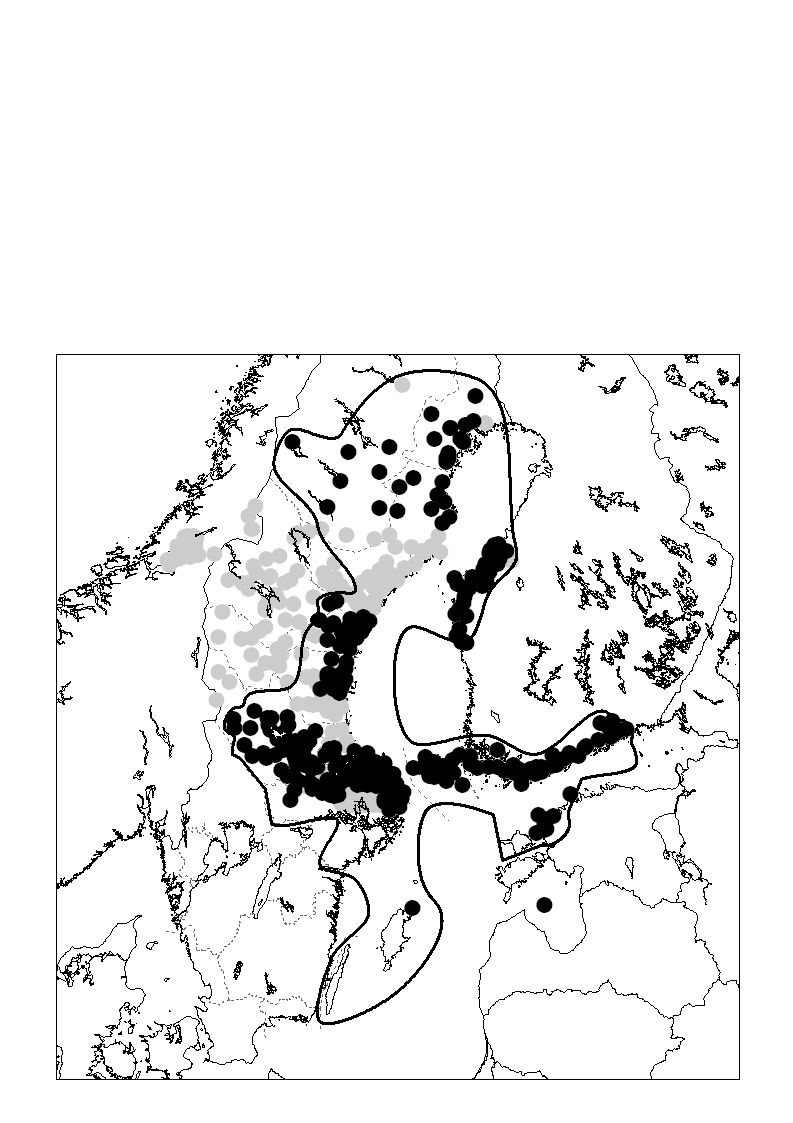
\includegraphics{figures_mod/image29}
\caption{Core areas of preserved dative use according to \citet{Reinhammar1973}.}
\label{map:29}

\end{figure}

\section{Conservative features of the Peripheral Swedish area}

Many of the conservative features of the Peripheral Swedish area are well-known and have been studied in detail. Most obviously, perhaps, is the retention of considerable parts of the morphology that were discarded in Central Scandinavian fairly early on.Thus, the old case system is at least partly preserved in several areas; this is particularly true for the dative case which is still alive in vernaculars in Dalarna, Härjedalen, Jämtland, Västerbotten and Norrbotten, with some remnants in Ångermanland and Medelpad (see \figref{map:29}). 

A three-way distinction between nominative, accusative, and dative is probably only found in the Ovansiljan area – the accusative case that has been claimed to exist in parts of Uppland is – or was – probably a general oblique case (Dahl \& Koptjevskaja-\citet{Tamm2006}). 

The vernaculars in Finland and Estonia do not feature the dative and accusative; one might perhaps think that the vicinity to Finnish and Estonian would favour the retainment of a complex case system. 

A three-gender system (rather than the two-gender system found in standard Danish and Swedish) has been generally preserved in the Peripheral Swedish vernaculars, but this is less significant, since it is true of most Peninsular Scandinavian vernaculars. 

In the pronoun system, one may note various forms of the 1\textsuperscript{st} person singular pronoun that contain the vowel \textstyleLinguisticExample{I, }such as \textstyleLinguisticExample{ik}, \textstyleLinguisticExample{ig}, \textstyleLinguisticExample{I}. It is somewhat unclear if this should be seen as a conservative feature or not – that is, whether the forms are derived directly from original “unbroken” forms such as Old Nordic \textstyleLinguisticExample{ek }or if they should be seen as reduced variants of “broken” forms like Standard Swedish \textstyleLinguisticExample{jag}. In any case, the \textstyleLinguisticExample{i}{}-forms are found, characteristically, in Norrbotten (although apparently restricted to Överkalix (Kx) in the north), most of Westrobothnian, all of Ovansiljan, and Malung (Vd). 

In verbal morphology, subject agreement is retained in Dalecarlian, in particular the Ovansiljan area, Northern Westrobothnian, and Norrbothnian. The distinction between singular and plural subjects is most widely marked but in Dalarna there is also special marking of the 1\textsuperscript{st} and 2\textsuperscript{nd} persons in the plural. It should be mentioned that verbs are also inflected for person and number in an area in Götaland (parts of Västergötland, Halland, and Småland) and in Gotland, Finland and parts of Estonia.

In phonology, the old \textstyleLinguisticExample{w}, corresponding to Central Scandinavian \textstyleLinguisticExample{v}, is retained, either only after consonants (including \textstyleLinguisticExample{h}, which later disappeared before \textstyleLinguisticExample{w/v}) or more generally in word-initial position (mainly Ovansiljan). Again, the same situation also obtains in parts of Götaland – much the same area as the one mentioned in the preceding paragraph but also including parts of Bohuslän. In another phonological development, Old Nordic \textstyleLinguisticExample{\=e} became \textstyleLinguisticExample{ä }in large parts of southern Scandinavia, but is retained in Norway, northern Bohuslän, northern Dalsland, Dalecarlian, Norrlandic and in the Trans-Baltic area (\citet[57]{Wessén1966}).

There are also a number of conservative syntactic features, some of which have not been properly described in the literature. I shall discuss two of them in the following sections.

\subsection{Infinitive constructions}
\label{bkm:Ref218337377}

Swedish employs an “infinitive marker” \textstyleLinguisticExample{att}, commonly pronounced [[254?]], which corresponds fairly well to English \textstyleLinguisticExample{to }with respect to its distribution. It is homographic to the complementizer \textstyleLinguisticExample{att} ‘that’ but in spoken language it is usually distinct from the latter, which is never reduced phonetically. Instead, the infinitive marker is homophonous with the reduced form of the conjunction \textstyleLinguisticExample{och} [ɔ], with which it is frequently confused. The two \textstyleLinguisticExample{att} also differ etymologically: the complementizer is considered to derive from the demonstrative pronoun \textstyleLinguisticExample{þat}, whereas the infinitive marker comes from the preposition \textstyleLinguisticExample{at} ‘to’ (cf. \sectref{sec:5.6}) and was first used in final constructions: 

\ea\label{}
\langinfo{Early Written Medieval Swedish}{}{}\\
\gll Han  är  i  sokn  farin,  siukum  \textbf{at} \textbf{hialpä.}\\
he  be.PRS  in  parish  go.PP  sick.DAT.PL  \textbf{INFM} \textbf{help.INF}\\
\glt ‘He has gone to the parish to help the sick.’ (Older Västgöta Law, \citet[136]{Wessén1956}) 
\z

In older forms of Swedish, the infinitive marker had a more restricted use than in Modern Swedish. In particular, we find bare infinitives as complements of adjectives as in:

\ea\label{}
\langinfo{Early Written Medieval Swedish}{}{}\\
\gll Bätra  är  dyrt  köpa  än  swälta.  \\
better  be.PRS  dearly  buy.INF  than  starve.INF  \\
\glt ‘It is better to buy dearly than to starve.’ (\citet[138]{Wessén1956})
\z

Wessén notes that in “Older Modern Swedish” the preposition \textstyleLinguisticExample{till} ‘to’ was frequently used as an infinitive marker. In fact, judging from the Cat Corpus material, cognates of this preposition are used very widely in vernaculars over most of Sweden (the old Danish provinces being an exception), and are in many cases the primary choice for an infinitive marker. The impression one gets is that \textstyleLinguisticExample{att, }when it does occur, is due to influence from the standard language. 

In addition, a few conservative vernaculars seem to retain the older pattern where the infinitive marker is used more sparingly. Compare the following adjective complement uses of infinitives from the Cat Corpus:

\ea\label{}
\langinfo{Älvdalen (Os)}{}{}\\
\gll E  war  do  fanta  me  it  so  litt\\
it  be.PST  then  devil\_take  me  NEG  so  easy\\
\gll \textbf{bigrip} \textbf{sig} o  kellinger,  itsä!\\
\textbf{understand.INF} \textbf{REFL} on  woman.PL  NEG\\
\glt  ‘It wasn’t easy, damn it, to understand women!’ (Cat Corpus)
\z

\ea\label{}
\langinfo{Nås (Vd)}{}{}\\
\gll Hä  va  då  innt  lätt  \textbf{begri´p} \textbf{sä} på  kvinnfôƚƚk  innt!\\
it  be.PST  then  NEG  easy  \textbf{understand.INF} \textbf{REFL} on  woman.PL  NEG\\
\glt ‘It really wasn’t easy to understand women!’ (Cat Corpus)
\z

\ea\label{}
\langinfo{\textit{Skelletmål} (NVb)}{}{}\\
\gll Hä  jer  väl  bäst  \textbf{pass} \textbf{sä.}\\
it  be.PRS  PRAG  best  \textbf{look\_out.INF} \textbf{REFL}\\
\glt ‘One had better look out.’ (Cat Corpus)
\z

\ea\label{}
\langinfo{Sävar (SVb)}{}{}\\
\gll Hä  tö  fäll  va  bäst  \textbf{akt}\textbf{  sä.}\\
it  ought\_to  PRAG  be.INF  best  \textbf{be\_careful\_about.INF} \textbf{REFL}\\
\glt ‘One had probably better look out.’ (Cat Corpus)
\z

These examples come from Dalecarlian and Northern Westrobothnian, the two most conservative regions in the Peripheral Swedish area. But \citet[99]{KällskogEtAl1993} also quote examples from Roslagen along the coast of Uppland, in slightly different syntactic contexts:

\ea\label{}
\langinfo{Väddö (Up)}{}{}\\
\gll de  håller  \textbf{spara}\\
it  keep.PRS  \textbf{save.INF}\\
\glt ‘it will keep if you save it [lit. it keeps to save]’
\z

\ea\label{}
\langinfo{Hållnäs (Up)}{}{}\\
\gll å  då  va  de  \textbf{fåljâs} åot\\
and  then  be.PST  it  \textbf{follow\_each\_other.INF} at\\
\glt ‘and then they had to go together’ 
\z

In other words, infinitive constructions are interesting in two ways: (i) the choice of infinitive marker is one feature where modern Standard Swedish differs from most vernaculars spoken in historical Sweden but is similar to Standard Danish and the vernaculars of the previous Danish provinces; (ii) the more restricted use of infinitive markers in general is still another conservative feature common to Dalarna and Västerbotten, extending also to Uppland. 

\subsection{Temporal subjunctions}

\citet{Vallmark1936} studied the distribution of temporal subjunctions in the Swedish dialect area. In modern spoken Standard Swedish the dominant translation of English \textstyleLinguisticExample{when} is \textstyleLinguisticExample{när}, which is also used as an interrogative adverb. A more formal or bookish alternative is \textstyleLinguisticExample{då}, whose major sense is ‘then’, and which is attested from Runic Swedish, where it appears to have been the primary choice. \textstyleLinguisticExample{När }started to be used as a subjunction in Written Medieval Swedish but was still relatively rare there. Its subsequent spread has not been complete: many conservative vernaculars lack it, or still use \textstyleLinguisticExample{då }as a natural alternative. Elfdalian goes its own way: \textstyleLinguisticExample{mes} (etymologically identical to Swedish \textstyleLinguisticExample{medan(s)} ‘while’) is used for singular events or periods in the past, \textstyleLinguisticExample{da(r)} (etymologically ‘there’) is used in other cases (Å\citet[152]{kerberg2012}). The Cat Corpus material on the whole confirms the picture given by Vallmark. Areas that retain \textstyleLinguisticExample{då} thus include the Dalecarlian area except Älvdalen; Norrland except southern Hälsingland, Gästrikland, most of Jämtland, \textit{Pitemål} and \textit{Nederkalixmål}; Ostrobothnia, Åboland and Nyland; Estonia; and northern Gotland (see \figref{map:30}). In Danish and Norwegian, \textstyleLinguisticExample{da} (etymologically the same as Swedish \textstyleLinguisticExample{då}) and \textstyleLinguisticExample{når} have a division of labour which resembles that between \textstyleLinguisticExample{als} and \textstyleLinguisticExample{wenn} in German. 

A similar story can be told about the verbs for ‘become’ (\citet{Markey1969}). In the late Middle Ages, the verb \textstyleLinguisticExample{bliva }(in Modern Swedish usually \textstyleLinguisticExample{bli}), with the original meaning ‘remain’ and emanating from Low German \textstyleLinguisticExample{blîwen}, started to take over the domain of the verb \textstyleLinguisticExample{varda} ‘become’ in Scandinavian. Again, the victory was only partial. While \textstyleLinguisticExample{bli }appears to reign supreme in most of Götaland (including Gotland), southern Finland and Estonia, even colloquial Standard Swedish as spoken in the Mälar provinces retains the alternative past tense form \textstyleLinguisticExample{vart} ‘became’ of \textstyleLinguisticExample{varda}, although all the other forms have disappeared. Most vernaculars of Svealand and Norrland also retain the supine form \textstyleLinguisticExample{vurti} (or similar). In some areas, however, the whole paradigm still exists (see \figref{map:32}), including large parts of Ovansiljan, Västerdalarna, Jämtland, Ångermanland, Västerbotten, Norrbotten, and Ostrobothnia.

The vernaculars of the Peripheral Swedish area preserve many lexical items that have been discarded in Standard Swedish. As an example of an item with a wide distribution, descendants of Old Swedish \textstyleLinguisticExample{fæghin }‘happy’ (cognate of English \textstyleLinguisticExample{fain}) may be mentioned as the standard counterpart of Swedish \textstyleLinguisticExample{glad}, e.g. Älvdalen \textstyleLinguisticExample{faingin}, Skellefteå \textstyleLinguisticExample{fajjen}, Färila \textstyleLinguisticExample{fäjjen}. (See \figref{map:32}.) What is less conspicuous are cases where some Swedish lexical item is missing from a vernacular and replaced by a synonymous word that also exists in Swedish. Consider the words for ‘find’ in Swedish. While \textstyleLinguisticExample{finna }is still quite viable in written Swedish, the natural alternative in most spoken varieties is \textstyleLinguisticExample{hitta}. Both these words were found with the same meaning in Written Medieval Swedish, although \textstyleLinguisticExample{finna} may reasonably be assumed to be the older word, with cognates in all branches of Germanic. Most pertinent to our context, we find \textstyleLinguisticExample{hitta} in the preface to the Upplandic Law:

\ea\label{}
\langinfo{Early Written Medieval Swedish}{}{}\\
\gll Hwat  ær  wi  \textbf{hittum} i  hans  laghsaghu\\
what  ever  we  \textbf{find.PRS.1PL} in  his  law.DAT\\
\gll ær  allum  mannum\\
that  all.DAT.PL  man.DAT.PL\\
\gll þarfflikt  ær  þæt  sætium  wir  i  bok  þæssæ.\\
useful  be.PRS  that  put.PRS.1PL  we  in  book  this.F.ACC\\
\glt ‘Whatever we find in his law that is useful for everyone we include in this book.’
\z

Turning now to the Cat Corpus, the Swedish version of the text contains three occurrences of the word \textstyleLinguisticExample{hitta} but none of \textstyleLinguisticExample{finna}, which is natural given the colloquial nature of the story. When checking how these are rendered in the other versions, we can see a widespread reluctance in the vernaculars to use the word \textstyleLinguisticExample{hitta}. At least nine versions use \textstyleLinguisticExample{finna} consistently, and about ten more do so in one or two cases of the three relevant ones. Except for Sotenäs (Bo), all these versions emanate from the northern side of \textstyleLinguisticExample{limes norrlandicus}, and among the more consistent cases we find, not unexpectedly, Älvdalen (Os) and the texts from the Northern Westrobothnian and Norrbothnian areas. In many of these texts, however, \textstyleLinguisticExample{hitta} shows up combined with the counterpart of the preposition \textstyleLinguisticExample{på} ‘on’ in the meaning ‘to think of, make up’:

\ea\label{}
\langinfo{Älvdalen (Os)}{}{}\\
\gll Wen  al  ig  itt  o  {i dag},  truä?\\
what  shall.PRS  I  find.INF  on  today  think.INF\\
\glt ‘What shall I think of today, I wonder.’
\z

It thus seems that \textstyleLinguisticExample{hitta} in its major use has never made its way into a significant number of Peripheral Swedish varieties. The natural conclusion would be that \textstyleLinguisticExample{hitta} was not part of the variety of Scandinavian which is the common ancestor of those varieties. In at least this respect, then, that language would differ from that of the Upplandic law. 

\begin{figure}[h]
%\includegraphics[height=.3\textheight]{filename.jpg}
\caption{Vernaculars with predominant \textstyleLinguisticExample{då }as temporal subjunction
 according to \citet{Vallmark1937}.  }
\label{map:6:30}
\end{figure}

\begin{figure}[h]
%\includegraphics[height=.3\textheight]{filename.jpg}
\caption{Degree of retainment of \textstyleLinguisticExample{varda} paradigm in the Swedish dialect area (\citet{Markey1969}). Black circles – full paradigm retained; grey circles – at least two forms retained; white circles – past tense only. }
\label{map:6:31}
\end{figure}

\begin{figure}[h]
%\includegraphics[height=.3\textheight]{filename.jpg}
\caption{(below) Degree of retainment
of \textstyleLinguisticExample{varda} paradigm
in the Swedish dialect area
(\citet{Markey1969}).}
\label{map:6:32a}
\end{figure}

\begin{figure}[h]
%\includegraphics[height=.3\textheight]{filename.jpg}
\caption{}
\label{map:6:32a}
\end{figure}

\begin{figure}[h]
%\includegraphics[height=.3\textheight]{filename.jpg}
\caption{Cognates of \textstyleLinguisticExample{fæghin} in the Cat Corpus (filled circles).}
\label{map:6:32b}
\end{figure}

\begin{figure}[h]
%\includegraphics[height=.3\textheight]{filename.jpg}
\caption{Distribution of \textstyleLinguisticExample{hitta} in Cat Corpus.}
\label{map:6:33}
\end{figure}
   
\section{The conservativity and innovativity indices}

We have looked at a number of “archaisms” and a number of innovations in the Peripheral Swedish area. Their distributions are not identical, but certain tendencies are visible and can be made even clearer by assigning two indices to each parish: one index of “conservativity” and one of “innovativity”, depending on how well the two types of features are represented in the vernacular in question. The definition of a conservative trait is one that is shared by the vernacular and the assumed common ancestor of all varieties in the Swedish dialect area, but which is not found in modern Standard Swedish. The definition of an innovative trait is one that is found neither in the assumed proto-language nor in modern Standard Swedish – and therefore must be assumed to have arisen through an innovation. 

The following features enter into the conservativity index:

\begin{itemize}
\item 

Preservation of original \textit{a} in positions where it has become \textit{å} in Swedish

\item 

Preservation of dative and/or accusative case in nouns

\item 

Preservation of original diphthongs

\item 

Preserved long stem vowels in cognates of Swedish \textit{natt} ‘night’ and \textit{döma} ‘judge’

\item 

Absence of temporal subjunction \textit{när}

\item 

No palatalization of \textit{k} and \textit{g} before front vowels in initial position

\item 

Absence of preposed definite article

\item 

Retainment of \textit{varda} paradigm

\item 

Preservation of \textit{w}
\end{itemize}
 

The following features go into the innovativity index:

\begin{itemize}
\item 

Presence of demonstratives of the type\textit{ han där} and \textit{he där}

\item 

Absence of neutral pronouns \textit{(h)ä(d)}

\item 

Presence of diphthongs \textit{ie} and \textit{yö}

\item 

Apocope

\item 

\textit{Pp} instead of \textit{mp }in words such as \textit{sopp} ‘mushroom’

\item 

Generic use of pronoun \textit{han}

\item 

Adjectival incorporation

\item 

Deletion of \textit{h}

\item 

\textit{(H)jär} ‘here’

\end{itemize}

The result is shown in Maps 34-35. 

\begin{figure}[h]
%\includegraphics[height=.3\textheight]{filename.jpg}
\caption{Distribution of conservative features in central and northern parts of the Swedish dialect
 area (darker circles -{}-higher conservativity index). }
\label{map:6:34}
\end{figure}

\begin{figure}[h]
%\includegraphics[height=.3\textheight]{filename.jpg}
\caption{Distribution of innovative features in central and northern parts of the Swedish
 dialect area (darker circles -{}-higher innovativity index). }
\label{map:6:35}
\end{figure}
 
 
As can be seen, the maps are similar enough for it not to be immediately obvious which map corresponds with the distribution of conservative vs. innovative features. From a visual inspection, conservativity and innovativity seem to be highly correlated. The correlation index turns out to be 0.62, which is perhaps not so impressive, but rises to 0.86 if we compare averages in dialect areas rather than values for individual parishes. The darkest areas of the maps are in Ovansiljan, northern Västerbotten and, to a lesser extent, Norrbotten. The most pronounced differences between the maps are found in Jämtland, which is more conservative than innovative, and Ostrobothnia, which is the other way around. 

What conclusion should be drawn from the similarity between the maps? In my opinion, the most parsimonious way of explaining the parallels between the conservative and the innovative features is that they originally had a shared larger distribution but were later pushed back by essentially the same kinds of processes. This means that the innovations must be old enough to have already been in place when these processes occurred. Given the general geographical picture, it appears that both the original spread of the innovative features and the later processes that obliterated them started in the same region, viz. in the Mälar provinces. 

Now, an objection may be raised that the choice of features is somewhat arbitrary. As for the conservative traits, I have mainly tried to choose ones where there is enough reliable information to make mapping possible, but I do not think it is possible to choose a set of features that would give a radically different picture. For the innovative features, the situation is a bit different. Here, I have to a certain degree deliberately chosen ones that fit the point of view I am arguing for. This is, I think, in fact legitimate insofar as I want to show that there is a coherent set of phenomena that show a definite pattern, suggesting a common history. Other innovations may not fit into that pattern, which can be seen as an indication of a different scenario. In particular, it does seem that certain phenomena spread, not from central Sweden, but rather from Norway. These include the use of preproprial articles and of \textstyleLinguisticExample{h}{}-genitives, two phenomena that most likely are connected with each other. 

\section{Notes on the historical background}
\subsection{Medieval Sweden}

According to the traditional view of Swedish history, during the Viking Age, if not earlier, the Svea ethnic group formed a kingdom with its centre in Uppland; this kingdom was fairly soon extended to also include the Göta ethnic group in central Götaland. developments in archaeology and history have modified this picture considerably. It is now thought that a stable central power was established in Sweden very gradually and probably not until the 13\textsuperscript{th} century. The existence of “kings” in Uppland from relatively early times seems well documented, but it is unclear how far their sphere of influence extended. During the 9\textsuperscript{th} and 10\textsuperscript{th} centuries, the town of Birka in Lake Mälaren (which was at this time part of the Baltic Sea) was the commercial centre of the Mälar region and was apparently part of a larger network including Hedeby in southern Denmark (present-day Schleswig-Holstein) and Kaupang in Norway. Around the turn of the millennium, Birka was replaced by Sigtuna farther to the east. The 11\textsuperscript{th} century is the time when most of the runic stones in Uppland were created. It appears that this was largely due to a “fashion” connected with the introduction of Christianity. There is evidence of Danish influence in Sigtuna during this period. According to the traditional account of the history of the Scandinavian languages, this was the time-point of the split between “East Nordic”, comprised of Danish and Swedish, and “West Nordic”, comprised of Norwegian and Icelandic. As I noted in \citet{Dahl2001}, the fact that Swedish and Danish seemed to go the same way – that is, that the same innovations were introduced in both Denmark and Sweden at the same time – is difficult to explain without assuming very intensive contact between the countries. It may be speculated that, in the Mälar provinces with Sigtuna as the centre, the introduction of Christianity was accompanied by the spread of a prestige dialect heavily influenced by Danish. 

The 12\textsuperscript{th} and 13\textsuperscript{th} centuries are somewhat paradoxical in the sense that the “Svea” kings were mainly based in Götaland, with power alternating between the leading families of Västergötland and Östergötland. It appears that since the royal title carried considerable prestige, it was a useful resource when consolidating the developing central power in Götaland even if it was associated historically with the Mälar provinces. At the same time, these provinces were less centralized, and the ruling group of magnates (\textstyleLinguisticExample{stormän}) there was apparently quite happy as long as the person who was nominally their King stayed in Götaland and did not interfere in their affairs. The process of Christianization went considerably faster and apparently more smoothly in Götaland than in Svealand. The fact that Svealand and Götaland had different monetary systems until the end of the 13\textsuperscript{th} century is another sign of the incomplete integration of the two regions. In fact, most of the visible events in Swedish history during this period took place in Götaland – one gets the impression that the Mälar provinces were some kind of backwater. At any rate, there is very little written documentation from this period. 

On the other hand, it does seem fairly clear that the Mälar provinces had a central part in one major economic and demographic development during this period, viz. the expansion of agriculture. \figref{map:36} shows the growth of permanently settled areas in Sweden from the Late Iron Age to the Late Middle Ages. As can be seen, it was during this period that large parts of the Peripheral Swedish area were settled. The same goes for the Swedish-speaking areas on the other side of the Baltic, which are not shown on the map. At least for the newly settled areas in Northern Sweden, it is probable that they received most of their new population from the Mälar provinces. Even areas that were already settled in the Iron Age, such as the peripheral parts of Uppland and the Middle Norrlandic provinces, greatly increased their population during this time (\citet{Broberg1990}), and it is reasonable to assume that there was considerable immigration from the central provinces. 

At least for the northernmost parts, the expansion seems to have continued during the first half of the 14\textsuperscript{th} century, when officially sanctioned colonization of the Lule and Pite river valleys took place, maybe in order to prevent Russian expansion plans in the area, and partly pushing back earlier Finnish settlements. In general, the expansion can be assumed to have been halted by the general agricultural crisis at the end of the Middle Ages, traditionally connected with the Black Death and a deterioration of the climate, and was not resumed until the 16\textsuperscript{th} century (\citet[248]{Myrdal2003}). Before this, however, other important things had happened.

Whereas the political leaders of Götaland had shown a certain lack of interest in Svealand in the 12\textsuperscript{th} and the beginning of the 13\textsuperscript{th} century, this changed under Birger Jarl, who was never King but effectively ruled Sweden as “jarl” during the years 1248-1266. He belonged to a leading family of Östergötland but is probably most well-known as the alleged founder of Stockholm, although his role in this may have been slightly exaggerated. (The continuous rise of the land had given Stockholm a very strategic position, since this was now the only entrance to Mälaren from the Baltic.)

What is clear is that Birger Jarl used quite brutal means to take control over the Mälar provinces, and that he realized the economic potential of this region, concluding among other things a treaty with the Hansa city Lübeck in order to promote the development of trade relations. The Mälar region was rapidly urbanized (see Map ). There were also considerable numbers of German merchants in the towns, and Low German was extensively used. German immigrants were also attracted to the Central Swedish mining district (“Bergslagen”), which was gradually growing in importance. A major factor in this development was the copper mine in Falun in southern Dalarna. At the same time, the previously quite important production of iron from bog and lake ore in northern Dalarna lost its significance. This may have contributed to the isolation of this area which in its turn may have cemented the linguistic differences between the Dalecarlian vernaculars and the rest of the Swedish dialect area. 

In the 14\textsuperscript{th} century, Denmark’s political influence grew, and in 1389, Denmark, Norway and Sweden were united in the Kalmar Union, which officially lasted until 1521, although in practice, Sweden was out of control for long periods. 

Turning now to linguistic developments during the Middle Ages, there is a virtual break in the record between the runic stones of the 11\textsuperscript{th} century and the first longer texts in Latin script in the 13\textsuperscript{th} century, although there is evidence for a continuous tradition of writing with runes (mainly on wood). From the 13\textsuperscript{th} century there are mainly provincial laws, the first longer text in Latin script emanating from the Mälar provinces is the Upplandic Law, which was promulgated by the King in 1296. (“Dalalagen” may be the oldest text from Svealand but its status is unclear.) 

The centre of the development of Written Medieval Swedish seems to have been Östergötland, more specifically the south-west part around the town of Vadstena, which was also the origin of the ruling families of the province. \citet[53]{Wessén1966} says that the Written Medieval Swedish was coloured by the Östergötland dialect\footnote{ “fornsvenskt skriftspråk är östgötskt färgat; det är väsentligen Vadstenaspråk” }, but one may surmise that it was the language of the élite that played the major role rather than that of the rank-and-file population. There has been little discussion of possible social variation in the language during this period, but given that society was highly stratified and that the ruling groups had intimate connections outside the area, it is to be expected that there were quite significant differences between the social classes. But Written Medieval Swedish, in particular the language of the legal texts, may also reflect older writing traditions.

There is relatively little dialectal variation in the provincial laws. This could be taken as an indication of the absence of such variation also in the spoken language, but in my opinion it rather suggests that there was in fact a relatively standardized way of writing such documents. We should therefore not expect, for example, the Upplandic Law to reflect spoken 13\textsuperscript{th} century Upplandic to any great extent. After all, it was produced by a royal commission (headed by Birger Persson, father of Saint Birgitta, recently appointed the Patron Saint of Europe). 

The strongest factor determining the further development of Swedish was undoubtedly the urbanization process and the development of trade relations. The strong influence of Low German on all the Scandinavian languages during this period, especially the vocabulary, is well known. Undoubtedly, the population of many Swedish towns was ethnically quite mixed, with a large proportion of Germans. It is also often pointed out that at least in Stockholm there was a fairly large number of Finnish speakers. It is highly probable that special urban varieties would have arisen in the Swedish towns and would have differed quite considerably from the ways people spoke in the surrounding countryside. Scholars such as Elias \citet{Wessén1954} have spoken of a “mixed language” as a result of German-Swedish contacts. But it is also likely that there were other non-local influences, since the population of the rapidly growing towns in the 13\textsuperscript{th} and 14\textsuperscript{th} century Mälar provinces would have also been recruited from other parts of Sweden. Birger Jarl’s taking control of the Mälar provinces must also have meant a movement of people from Östergötland to Stockholm and other towns in the area, and this may have especially had consequences for the prestige variety.

In addition, the role of Danish has probably been underestimated. The 19\textsuperscript{th} century scholar Esaias Tegnér, Jr. voiced the opinion that “even if, as is natural, Swedish received many loans directly from German during the Low German period…, it is the Danish influence during the period of the Kalmar union which to a quite essential extent has contributed to the establishment of such Low German words and to the form in which they appear”.\footnote{ “En granskning af de tyska lånorden i vårt språk har bibragt mig det intrycket, att om ock svenskan naturligtvis under den lågtyska perioden (intill reformationstiden) mottagit många lån omedelbart från tyskan, så är det likväl i ganska väsentlig grad danskarnas inflytande i Sverige under Kalmarunionens tid, som bidragit därtill att dylika lågtyska ord blivit bofasta hos oss och att de uppträda i den form, som vi finna dem hava.” (\citet[159]{Tegnér1889})} Tegnér points to the high degree of correspondence between the Low German grammatical and lexical elements in Danish and Swedish and to the fact that the same deviations from the original Low German forms tend to show up in both languages. Such differences that are found, he says, are usually attributable to later High German influences. I checked Tegnér’s claims by looking at the words listed as Low German loans in \citet{Hellquist1922}; as it turns out, a very high proportion (perhaps something like 90 per cent) do exist or have existed also in Danish. Scholars after Tegnér, however, have not paid too much attention to his hypothesis. \citet{Wessén1954} is sceptical: according to him, the high degree of correspondence, which he does not deny, can be explained by the common “cultural and linguistic preconditions” for borrowings in Danish and Swedish. I would personally tend to side with Tegnér on this issue. It is, furthermore, possible to establish quite a long list of points where Standard Swedish and urban Central Swedish join Standard Danish against most of the vernaculars in Peninsular Scandinavia, at least those north of the Southern Swedish/East Danish dialect area, such as the restructured gender system, the feminine definite suffix\textit{ {}-}\textstyleLinguisticExample{en}, the use of \textstyleLinguisticExample{att} (rather than \textstyleLinguisticExample{till}) as an infinitive marker and \textstyleLinguisticExample{man} as a generic pronoun, consistent preposed placement of possessive pronouns etc. 

It is commonly said that Standard Swedish arose from the dialects of the Mälar region, but it is often not made clear exactly which these dialects were. \citet[67]{KällskogEtAl1993}, in their discussion of the similarity between Standard Swedish and Upplandic, claim that the base for the former is to be found in medieval “high-status dialects, primarily Upplandic and \textit{östgötska} [the speech of Östergötland]”.\footnote{ “Stommen i detta språk utgjordes av folkmål med hög status, främst uppländska och östgötska…”} Thus, they say, it is not the case that Upplandic has been influenced by the standard language in Stockholm and Uppsala, it is rather the other way around. The Swedish expression they use for ‘high-status dialects’, “folkmål med hög status”, sounds almost like an oxymoron, given that “folkmål” is usually understood as denoting rural, non-standard varieties. In fact, their claim does not make a lot of sense if the flow of influence is not supposed to go from rural to urban varieties. In the next section, we shall look more closely at the dialect situation in Uppland.

\begin{figure}[h]
%\includegraphics[height=.3\textheight]{filename.jpg}
\caption{Growth of permanently  settled areas between approx. 800CE and 1350CE. }
\label{map:6:36}
\end{figure}

\begin{figure}[h]
%\includegraphics[height=.3\textheight]{filename.jpg}
\caption{Cities and towns in the Mälar region  in the late 13th century. }
\label{map:6:37}
\end{figure}

\begin{figure}[h]
%\includegraphics[height=.3\textheight]{filename.jpg}
\caption{Distribution of population in present-day Uppland.}
\label{map:6:39}
\end{figure}

 
\begin{figure}[h]
%\includegraphics[height=.3\textheight]{filename.jpg}
\caption{Uppland with “high-activity” areas  and medieval churches (black circles represent churches built 1000-{}-1250, grey circles churches built 1250-1500; left hatching  {}-{}- hundreds with {\textgreater}20 runic stones, right hatching  {}-{}- {\textgreater}50 per cent land with tax-relief in the mid 16\textsuperscript{th} century).}
\label{map:6:38}
\end{figure}

  

\subsection{Uppland}

To understand the dialectological situation in Uppland, it is of some importance to relate it to the administrative and demographic structure of the province.

The present-day province of Uppland has, strictly speaking, never functioned as an administrative unit. The judicial province (\textstyleLinguisticExample{lagsaga}) of Uppland that was created in 1296 also included the province of Gästrikland, and was formed by merging three so-called “folklands”, Fjädrundaland (Fjärdhundraland), Tiundaland, and Attundaland. These names mean “the land of four (ten, eight) hundreds” and refer to the number of \textstyleLinguisticExample{hundare}\textstyleLinguisticExample{,}\footnote{ The word \textit{hundare} corresponds etymologically to English \textit{hundred}\textit{,} used in medieval England as a term for a division of a shire The \textit{hundare} were later on identified with the judicial districts called \textit{härad}.} smaller administrative units, suggesting that the names were created as a bureaucratic measure from above rather than developing naturally. The coastal region nowadays called Roslagen had a somewhat uncertain status: it was divided into two halves, referred to as “Norra Roden” and “Södra Roden”, and loosely attached to Tiundaland and Attundaland, respectively. 

The population of Uppland has always been unevenly distributed. \figref{map:39} shows the present-day situation, with a heavy concentration in the urban areas around Stockholm and Uppsala. The medieval distribution was not that different, in fact. The hatched areas in \figref{map:38} (after \citet{Broberg1990}) show the following indicators of social stratification (and thus, presumably the areas with the greatest economic activity and densest population) in earlier times: (i) the hundreds with more than 20 runic stones, (ii) the hundreds which had more than 50 per cent land with tax-relief (that is, land owned by the state, the church or the nobility) in the mid 16\textsuperscript{th} century. It is somewhat remarkable that these two indicators coincide almost completely, and are not too different from what we find today. 

\figref{map:38} also shows the medieval churches in the area, according to the database of the Swedish National Heritage Board (\href{http://www.raa.se}{{www.raa.se}}). These data are of some interest because they show a possible model for the way linguistic innovations may have spread in this period. We can see that there is a concentration of early churches in the southern part of the hatched area, whereas church construction in the Late Middle Ages took place to a much larger extent in the peripheral areas.

The conclusion that can be drawn is that medieval Uppland, like Uppland of today, can be understood as having consisted of a centre in the middle south, in the areas adjacent to Lake Mälaren, and a periphery around it. Crucially, this persistent division cross-cuts the old administrative division into folklands, as can be seen when comparing \figref{map:38}-\figref{map:39} with \figref{map:40}. The structure of Uppland is somewhat like (half) a pizza, with each folkland representing one slice, all of which meet in the most densely populated area in the south in the immediate vicinity of the medieval towns Uppsala and Sigtuna. Each folkland itself thus consists of a central and a peripheral part. 

 The first and in some ways still most complete account of the Upplandic dialects is that of \citet{Kruuse1908}.\footnote{ Kruuse says that he bases his account on word lists collected in a survey led by A. Erdmann, in addition to various written works. (The later fate of these word lists is unclear.) } Kruuse is somewhat hesitant to divide Uppland into dialect areas, being well aware that “the area of one linguistic feature very seldom coincides with the area of another, and strictly speaking we cannot speak of a certain number of dialects with definite borders”. After having stated this reservation, he presents a division of the province into four areas, based on a number of important isoglosses. There is a map provided with Kruuse’s article, but it shows the isoglosses rather than the areas – neither Kruuse nor anybody else seems to have drawn a map of the areas themselves, so \figref{map:40} is my own reconstruction from the description in Kruuse’s text. 

A different division is given by \citet[1194]{Hesselman1920} in his article on Upplandic dialects in the encyclopedia \textstyleLinguisticExample{Nordisk familjebok}. He proposes to divide the Upplandic vernaculars “in three larger groups, whose borders by and large follow those of the ancient folklands”.\footnote{ “En god indelning är den, som sammanför upplandsmålen i tre större grupper, hvilkas gränser i stort sedt följa de gamla uppländska folklandens.” } This statement is echoed in later treatments. Thus, in \citet[75]{KällskogEtAl1993}, it is said that Uppland can be divided “into three dialect areas, which to some extent coincide” with the folklands.\footnote{ “Landskapet Uppland kan grovt delas in i tre dialektområden som i någon mån sammanfaller med de tre s.k. folklanden från vikingatid och medeltid…” } The change from “by and large” to “to some extent” may reflect a certain uneasiness on part of the authors. In their ensuing presentation, however, the names of the folklands are used as labels of the three areas, with which they are in practice identified. In my opinion, such a practice is rather misleading. As can be seen from \figref{map:40}, the placement of the borders of the folklands, does not coincide very well with the areas proposed by Kruuse, and indeed, if one looks at the borders of individual phenomena, they tend not to honour the actual folkland borders. What is particularly important here is that three of Kruuse’s areas that “to some extent” coincide with the folklands (Areas 1-3) are actually mainly located on their periphery, while Kruuse’s Area 4 equals the demographic and economic centre of the province, which as we have seen, also includes the pivot points of all three folklands. Note that Kruuse’s Area 4 is wholly included in the central area indicated in \figref{map:38} and in fact follows its borders relatively closely, except in the east. This does not warrant the conclusion that Kruuse’s areas directly reflect the demographic and economic situation in the Middle Ages. The explanation is rather that the centre-periphery division of Uppland has been relatively constant over the last millennium and that it is this division that underlies the modern dialectological make-up of Uppland, being a result of the expansion of innovations from a centre towards a periphery as much as an ancient division into subprovinces. In particular, some of the borderlines drawn by Kruuse may be snapshots of a moving boundary.

\citet[77]{Wessén1966}, having first pointed to the possibility of an influence of “German sound formation and German linguistic habits” on medieval Stockholm speech, says that medieval documents suggest that the spoken language in Stockholm was “to a striking extent” coloured by Central Swedish and Götamål (see \sectref{sec:2.3.2}). (He explains this by immigration from the “inner Mälar provinces”, but does not say where the Göta influence would come from.)

Among the traits characterizing parts of Uppland, there is a subset which shows some interesting and partly baffling characteristics. To start with, most treatments, beginning with Kruuse (or even earlier, in \citet{Rydqvist1868}), tell us that there have been changes in the pitch accent systems in parts of Uppland: the acute accent has been generalized in the northeast (the eastern part of Kruuse’s Area 2), while the grave accent is generalized in large parts of southern Uppland and also in the eastern part of Södermanland (most of Kruuse’s Area 4 and parts of his Area 1, see \figref{map:41}). The generalized grave accent is discussed in some detail in \citet{Nyström1997}.\footnote{ It is not always clear if the generalization means that all words are pronounced with a grave accent or that just more of them are than in the standard language. Thus, Nyström enumerates some standard minimal pairs such as \textit{ánden} ‘the duck’: \textit{ànden} ‘the spirit’ and says that they are all pronounced with a grave accent, and then adds that “also polysyllabic words such as \textit{betàla} ‘pay’, \textit{indiàner} ‘indians’…” are pronounced “more often” with a grave accent. } (For an account of the present-day situation, see \citet{Ericsson2006}). Nyström mentions two logical possibilities: either the grave accent was productive at the time when the definite article became an affix (see \sectref{sec:3.1.4}) and monosyllabic words became bisyllabic through the insertion of a “svarabhakti” vowel, or the generalization is a later innovation, taking place some time between the changes just mentioned and the mid 19\textsuperscript{th} century, when the phenomenon was first documented. In the latter case, which he seems to lean towards, it is plausible to assume, he says, that the generalized grave accent was also found in the urban varieties spoken in Stockholm (as was also suggested by \citet{Otterbjörk1982}) and that maybe Stockholm was in fact the origin of the development. if the contiguous area shown in \figref{map:41} could not include its geographical centre, Stockholm, this would be hard to explain “from the point of view of dialect geography”. A possible scenario would then be as follows: the “massive Low German influence” in the city during the late Middle Ages would have triggered the coalescence of the two pitch accents, and this would then have spread to neighbouring areas. Later on, the pitch accent distinction would have been re-introduced in Stockholm during the expansion of the city from the 18\textsuperscript{th} century onwards, as a combined result of the influx of people from other parts of the country and the rise of a national spoken standard. In the context of our discussion, this hypothesized development is highly interesting in that it illustrates how innovations from a centre could be canceled by later spreads from the same centre. In fact, there are a few more features that have a rather peculiar distribution in the Mälar area and which could be ascribed to similar processes. 

One such feature is the preservation of \textstyleLinguisticExample{k} before initial front vowels, reported by \citet{Kruuse1908} (he gives examples such as \textit{kepp} ‘stick’ and \textit{körä} ‘drive’ from the Vätö vernacular). This feature was found in areas almost enclosing Stockholm (see \figref{map:41}) but has probably more or less disappeared by now. It certainly looks as a conservative feature, but the donut shape of the area would rather suggest an expansion from Stockholm outwards. In the speech of the capital, it might be due to foreign, possibly Danish, influence.

The other feature to be noted here is the definite endings of feminine nouns. In Written Medieval Swedish, the definite form of a word such as \textstyleLinguisticExample{bok} ‘book’ was \textstyleLinguisticExample{bokin}. In the modern vernaculars of most parts of Sweden and Norway, feminine words would take a definite suffix\textit{ {}-a} or\textit{ {}-}\textstyleLinguisticExample{i}, but there is an area to the north and south of Lake Mälaren where the ending is\textit{ {}-}\textstyleLinguisticExample{en}. In \figref{map:41}, the borderlines of this area are shown in accordance with \citet{Modéer1946}. This is often seen as a conservative feature, but the fact that it is also found in Denmark and the South Swedish dialect area, as well as in Standard Swedish, suggests that it could also be the result of an import from the south into the Stockholm area, from which it then expanded. In this connection, it is not irrelevant that the \textit{{}-en} ending tends to be connected with a breakdown of the old three-gender system and the rise of the new two-gender one – a development which is common to Stockholm speech and varieties in Denmark and Southern Sweden.

It may be seen as a difficulty for this hypothesis that the \textit{{}-en} area extends as far as Gästrikland in the north. On the other hand, the distribution of the \textit{{}-}\textit{en} ending is not too different from that of the generalized grave accent, as described by Kruuse, which goes at least as far north as the border between Uppland and Gästrikland.

It is not excluded, however, as assumed by \citet[239]{LindströmEtAl2006}, that even if there is influence from the south in the high-prestige varieties, the\textit{ {}-}\textstyleLinguisticExample{en} ending in the more peripheral parts of the area is a conservative trait.

As was noted above, the settlement of the Peripheral Swedish area took place mainly during the period between 1200 and 1350. If the assumption that the Mälar provinces were the major contributors to this expansion, we might expect the Peripheral Swedish vernaculars to reflect the varieties that were spoken in those provinces in the 13\textsuperscript{th}{}-14\textsuperscript{th} centuries. This would also be in accordance with the view expounded above in \sectref{sec:6.1}, which included the assumption that at least the more standard varieties of the present-day Mälar provinces would preserve the traits of those varieties to a significantly lesser extent. While the phenomena that were at the focus of interest in Chapters 3{}-5 are hardly found in the Mälar provinces at all, there are, as we have already seen, quite a few other traits characteristic of the Peripheral Swedish vernaculars that also show up in at least parts of Uppland and even further south, at least in earlier times. One might hope that the geographical distribution of those traits in the Mälar provinces would tell us something about the origin of the people who settled the periphery. What we see, however, is that the traits in question tend to show up in the peripheral parts, that is, primarily northern and eastern Uppland – this goes for innovations such as the distribution of \textstyleLinguisticExample{h}{}-pronouns, medial affrication, and the use of \textstyleLinguisticExample{han} as a generic pronoun, and for conservative traits such as post-position of possessive pronouns, omission of infinitive markers, retained consonant clusters such as \textstyleLinguisticExample{mb }(as in\textstyleLinguisticExample{ lamb} ‘lamb’)\textit{ }and various others. It is less likely that these somewhat sparsely populated parts of Uppland were the major source for the emigration to the Peripheral Swedish area – rather, they were themselves at least partly settled during the same period (\citet{Broberg1990}). The settlers will have come primarily from the more populous regions in the southern and western parts of Uppland, and the reason that there are not more similarities between the vernaculars of those areas and the ones in the Peripheral Swedish has to be that those similarities were obliterated under external influence. 

In their treatment of the critical historical period in the Mälar provinces, \citet{LindströmEtAl} argue for a somewhat different picture. According to them, the resistance against Birger Jarl’s strivings to control the Mälar provinces was concentrated in the southwestern part of Uppland – Fjädrundaland (Fjärdhundraland) (which also may have included parts of Västmanland at the time). They argue that this area is characterized by a linguistic conservatism, assumed to reflect the unwillingness of the medieval population to accept foreign innovations. Moreover, they say that there is evidence that the emigration to the peripheral areas was concentrated in this area: “From a purely linguistic point of view there are several common traits to these newly settled regions and precisely the peculiar dialect of the Fjärdhundra area.”

These claims are a bit unexpected in the light of what I have just said about the distribution of linguistic traits in Uppland. The empirical evidence they provide also turns out to be a bit thin. The trait that they discuss in some detail\footnote{ The other trait they mention is the “pure å-sound for old short {\textgreater}o{\textless}” (“det rena å-ljudet för gammalt kort {\textgreater}o{\textless}” (\citet[315]{LindströmEtAl2006}). I am not sure what this refers to, possibly to the pronunciation of the feminine plural ending -\textit{o}\textit{r}.} is the definite feminine noun ending \textit{{}-en} discussed above, which is in their opinion a conservative trait in Fjädrundaland. Even if we assume that they are right on this point, the\textit{ {}-}\textstyleLinguisticExample{en} ending can hardly be used as evidence for the connection between Fjädrundaland and the peripheral areas, since the feminine definite suffix generally ends in a vowel rather than in\textit{ {}-}\textstyleLinguisticExample{n} in the Peripheral Swedish vernaculars except the vernaculars spoken in Finland.  In most of the area, the general ending is\textit{ {}-a}, the exception being the Ovansiljan area, where it is\textit{ {}-}\textstyleLinguisticExample{i/-e }or (nasalized)\textit{ {}-}\textstyleLinguisticExample{\k{i}}\textstyleLinguisticExample{/-e;}. In this respect, there is a connection between Ovansiljan, coastal vernaculars in Roslagen (Uppland) and Södertörn (Södermanland) as well as Gotland, where the ending\textit{ {}-}\textstyleLinguisticExample{i} is also found. Given that\textit{ {}-}\textstyleLinguisticExample{i} is also found as a feminine definite ending in some vernaculars in the inner parts of Norway, the total picture of the distribution of feminine definite suffixes is rather confusing. 

In fact, the Ovansiljan area shares other traits with the coastal areas of Uppland and Södermanland that are not found further north in Sweden, including the diphthongs \textstyleLinguisticExample{ie} and \textstyleLinguisticExample{yö}, corresponding to Swedish long \textstyleLinguisticExample{e} and \textstyleLinguisticExample{ö}, and the disappearance of the \textstyleLinguisticExample{h} phoneme, although the last-mentioned feature is admittedly probably a late innovation in the Dalecarlian area. In any case, the linguistic evidence for an early strong connection between south-western Uppland and Dalarna, as suggested by \citet[237]{LindströmEtAl2006}, and as might prima facie seem natural from the geographical point of view, is rather scanty.\footnote{\citet[237]{LindströmEtAl2006} also indirectly admit this by saying that if the contact between Uppland and Dalarna had not been “cut off” by the immigration to the high-mobility mining district, the connection would have been “much more apparent” (“mycket mer uppenbart”).}

 

\begin{figure}[h]
%\includegraphics[height=.3\textheight]{filename.jpg}
\caption{Kruuse’s dialect areas and the Upplandic folklands}
\label{map:6:33}
\end{figure}

\begin{figure}[h]
%\includegraphics[height=.3\textheight]{filename.jpg}
\caption{Kruuse’s dialect areas and the Upplandic folklands.}
\label{map:6:40}
\end{figure}

 
\begin{figure}[h]
%\includegraphics[height=.3\textheight]{filename.jpg}
\caption{Some mysterious dialect phenomena in the Mälar area.}
\label{map:6:41}
\end{figure}

 
 
\chapter{Concluding discussion}

What we have seen in this book is a variety of developments within the grammar of noun phrases in the vernaculars of the Peripheral Swedish area. Some of these developments are astonishingly uniform across this vast area, suggesting an early origin. But at the same time we find diversity in details, and in some domains, perhaps most strikingly in the marking of possessive constructions, a bewildering number of alternative ways of expressing the same content. 

What can we find here that is of interest beyond the purely dialectological description of phenomena? 

Let us begin with a look at the grammaticalization of definite articles. This is a topic that has been studied in some detail, but the particular patterns we find in the Peripheral Swedish area are relatively unusual typologically and have not been studied from a cross-linguistic or diachronic point of view. It was shown in Greenberg’s classical work (\citet{Greenberg1978}) that definite articles can develop beyond what we would normally think of as their final stage of development, the “full-blown” definite article as we find it for instance in English. In the cases discussed by Greenberg, the articles eventually develop into general affixes on nouns, carrying gender and number information. Another possible further stage is found in the “specific” articles in Austronesian languages (see \sectref{sec:3.1.3}). In Peripheral Swedish vernaculars, we now see another development: definite articles – or definite suffixes on nouns – are extended to a number of uses commonly associated with articleless indefinites – non-delimited (“partitive”) uses, uses with quantifiers and low-referentiality uses of singular count nouns. I hypothesized in \chapref{chap:3} that these developments, for which the clearest parallels are found in Moroccan Arabic, are mediated by generic uses of definite noun phrases, which are more pervasive in the Peripheral Swedish vernaculars than in Central Scandinavian. Evidence from Romance, in particular Italian and Italian vernaculars, was given in support of this. 

As I argued in \citet{Dahl2003}, there have been several different grammaticalizations of definite articles in the North Germanic area, and in a large part of the area, this led to competition between preposed and suffixed articles, with different solutions in different varieties. The notion of a “buffer zone” which was used in \citet{Stilo2004} to refer to the more general phenomenon of a typologically “inconsistent” zone between two areas with consistent typological patterns.  may be applied here.

In the Peripheral Swedish area, the suffixed articles are in general the strongest, the preposed being rather marginal, but we also find “non-standard” developments of demonstratives into preposed definites, a somewhat neglected topic in the literature. 

Adjective incorporation, which is another pervasive phenomenon in the Peripheral Swedish area, represents a type of incorporation which differs from other more well-known cases such as noun incorporation. Most notably, it is in many varieties obligatory in the sense that it is the only way of combining an adjective with a definite noun. Regrettably, the origin of the incorporation construction remains rather obscure, and due to the lack of data from earlier periods we may never be able to find out exactly how it came about. It does seem, however, that the incorporating construction arose through a process in which combinations of weak attributed adjectives with apocopated endings and definite head nouns were reinterpreted as compounds. In the vernaculars where incorporated adjectives compete with syntactic constructions, the division of labour between the alternatives is reminiscent of that between, for example, preposed and postposed attributive adjectives in Romance, in that incorporated and preposed adjectives tend to be chosen primarily from the set of “prototypical” adjectives identified by \citet{Dixon1977}. Further research is needed to elucidate the principles by which choices between alternative attributive constructions are made in the languages of the world.

A common feature to the phenomena studied in this book is that these are innovations, relative to older forms of North Germanic, and are usually more or less restricted to the Peripheral Swedish area or parts of it. This also means that as the standard language – Swedish – advances or at least increases its influence on local varieties, the features in question tend to retreat and eventually disappear. This is a kind of situation which has not received due attention in the literature on grammatical change (see (\citet{Dahl2004}) for a discussion). What is peculiar about it is that it represents a seeming reversal of the original grammaticalization process, and could thus be said to be a kind of degrammaticalization – a notion which has usually been taken to necessarily involve a development from grammatical to lexical morphemes. More concretely: in some language variety, a grammatical construction is extended to a new use, but after some time this use disappears under the pressure of some neighbouring language variety in which the original change never took place. An interesting problem then is what exactly happens if the reversal takes place gradually rather than all at once – is this process in any way comparable to the original grammaticalization?

There is in fact some evidence to suggest that this is the case. More specifically, if we look at the extended uses of definite forms in the Peripheral Swedish area, there is at least one fairly clear case where the contexts which survive longest when the uses are disappearing are those that most probably were the first to appear when the extension took place. It was suggested in \chapref{chap:3} that the non-delimited uses of definite forms developed out of generic uses of such forms. It was also noted that there are intermediate cases where it is possible to choose between a generic noun phrase and an indefinite one, and that such cases are presumably the bridgehead for the further expansion of definites into the non-delimited territory. For example, both in Standard Italian and Italian vernaculars, definite noun phrases corresponding to English bare NPs are more likely to show up in habitual contexts. Thus, \REF{336}(a) is more natural than (b).

\ea\label{}
\langinfo{\label{bkm:Ref173317986}Italian}{}{}\\
\ea {
\gll Papà  beve  \textbf{la} \textbf{birra} ogni  mattina.\\
father  drink.PRS.3SG  \textbf{DEF} \textbf{beer} every  morning\\
\glt ‘Father drinks beer every morning.’ 
}

\ex {
father  PROG.3.SG  drink.GER  \textbf{DEF} \textbf{beer} exact  hour\\
\glt ‘Father is drinking beer right now.’ (Pier Marco Bertinetto, pers.comm.)
}
\z 
\z

But in a similar way, in the vernacular of Sollerön (Os), \REF{54}, repeated here, the choice of the definite form induces a habitual interpretation:

\ea\label{ex:54}
\langinfo{Sollerön (Os)}{}{}\\
\gll An  drikk  \textbf{mjotji.}\\
he  drink.PRS  \textbf{milk.DEF}\\
\glt ‘He drinks milk.’ (questionnaire)
\z

The difference between the two cases is that for the vernacular of Sollerön, we have reason to assume that \REF{54} represents a receding use, that is, it is likely that the definite forms were used more generally in non-delimited contexts, whereas there is no such evidence for Italian – rather, we have to see Italian as a language which has undergone only the initial stages of the extension of definite marking that we see in the Peripheral Swedish area. 

It is not unreasonable that the contexts first hit by an expanding construction should also be the last ones to remain when the use of that construction contracts. More empirical evidence is needed, however, to establish whether this is a general phenomenon. I want to mention here a somewhat similar case from the literature on language change. In their discussion of Cappadocian Greek, \citet{ThomasonEtAl}, quoting \citet{Dawkins1916}, note that the use of the definite article has “declined drastically”. That this has taken place under the influence of Turkish rather than independently is seen from the fact that the Greek article is retained “only in the single morphosyntactic context where Turkish marks definiteness – on direct objects (i.e., in the accusative case)”. This is not a perfect parallel, and it is also not clear that the accusative in Turkish is a marker on definiteness on direct objects rather than a direct object marker on definite NPs. However, what it shows is the following. Differential marking of definite and indefinite objects commonly arises as an extended use of some case marker or adposition, e.g. a marker of indirect objects. But as we see here, there is another possibility where, under the influence of patterns in a neighbouring language, such marking is the result of shrinking the domain of use of a grammatical morpheme. 

A somewhat related problem arises with the incorporated adjectives. As we have seen, in some areas, adjectival incorporation is restricted to a few “prototypical” adjectives such as ‘big’ and ‘new’. At least in the Ovansiljan area, this appears to be a fossilized state of a more general construction which was used more indiscriminately with definite attributive adjectives, and which has been pushed back by a competing construction (with a demonstrative pronoun in the function of preposed article). The question is if this is the only way in which such lexically restricted incorporation can arise. In some Romance languages, some “prototypical” adjectives, when preposed to a noun, behave in a way that looks very much like the incorporated adjectives of Peripheral Swedish in that the final ending may be elided, as in Spanish \textit{un gran hombre} ‘a great man’ (as compared to \textit{un hombre grande }‘a big man’, with the adjective in a non-reduced form). In the absence of evidence that this has been a more general process, it seems most natural to assume that it is a process that has hit these particular adjectives exclusively. Likewise, it is questionable whether adjectival incorporation has ever been a more general process for instance in the varieties of Norwegian where it occurs with a few adjectives such as \textit{ny} ‘new’. It would thus seem that there is more than one path to the synchronic state in which prototypical adjectives enter into a tighter relationship with a head noun. What I have said here does not preclude that there may be other aspects of the developments that make the patterns in Scandinavian and Romance differ (such as a differentiation in meaning between the preposed and postposed variants). 

The other field for which this investigation may be relevant is the history of the Scandinavian languages. Traditional accounts of this history tend to see it as a linear development in which the various vernaculars grow out of relatively unified older stages; for the ones spoken within the original Swedish provinces, it is usually assumed that they derive from what is referred to as \textit{fornsvenska} or “Old Swedish”, which was gradually differentiated into Svea and Göta vernaculars. However, the traits that were involved in this differentiation, such as the lengthening of short syllables, are relatively late and can be attributed to the period after Birger Jarl’s taking control of the Svea provinces – which among other things is reflected in the fact that these developments were only partly implemented in the Peripheral Swedish area. On the other hand, a large number of innovations, including the ones which this book focuses on, are widespread in the same area and also sometimes other more central parts of the old Svea provinces. Historically, some of these developments, such as the innovations of the pronoun system, can be shown to go back to medieval times, and must thus be the result of an early spread in the Svea area of influence. Since these developments show a very different geographical pattern from the innovations that differentiated Svea vernaculars from the Göta ones, it is unlikely that they took place at the same time or spread along the same routes. Rather, I would argue, we should assume that they are older, having spread during a period when the influence from the south had not yet become very strong in the Mälar provinces, from which they were later pushed back. The development of the language of the Mälar region has thus not been linear in the sense that the modern varieties of that region are to be seen as direct descendants of the varities spoken there in the early Middle Age. If this is the case, one may wonder why it has not been obvious to earlier researchers. It may be noted that the assumption of a linear development fits well with the traditional view of Sweden as having always had a natural political and economic center in Svealand. The more recent view, that the main center of power has at times been located in Götaland, can be more easily combined with a non-linear view of linguistic developments. It may also be the case that the focus on sound change in traditional historical linguistics has detracted attention from phenomena of a more grammatical (particularly syntactic) character, phenomena which the Peripheral Swedish developments tend to demonstrate.

I thus hope to have demonstrated that the study of grammatical phenomena in traditional non-standardized varieties can uncover typologically interesting patterns as well as suggest paths of development and spread of linguistic phenomena. 


 
\chapter{Appendix: quotations from older texts}
\section{Some cases of extended uses of definite articles in Written Medieval Swedish}



 
\subsection*{Mistha klöffwana}
 
\begin{quotation}
%\begin{styleBodyTextFirst}
Misther falken klöffwana, Tha tak paper oc \textstyleLinguisticExample{tänth elden thär j} oc bren the thaana som klöffwen wil aff falla, oc smör sidhan äffther mädh honagh oc bint bombas thär wm j nyo dagha etc:-

%\end{styleBodyTextFirst}

\end{quotation}
[S7], \#142

\subsection*{Göra en sten som tänder eld aff spwteno} 
\begin{quotation}

%\begin{styleBlockQuoteHeading}

%\end{styleBlockQuoteHeading}

%\begin{styleBodyTextFirst}
Tak osläktan kalk tw lod, tuciam som ey är tilredh ij lod, salpeter ij lod, brennesten ij lod, camfora ij lod, calamitam ij lod, Stötis alth ganskans granth oc sammanblandis sictandis gönom en haardwk. Sidan läth thet alth j en posa aff nyth oc täth lärofft trykkiandis harth samman oc täth före knytandis, sidan läg then posan j ena leer krwko, oc eth lok lwtera tättelika oc starkelika affwan wpp swa ath jngen ande kan wthkomma, oc säth swa pottona äller leerkrwekona j oghnen \textit{görandis eldhen} wmkringh, oc när alt är bränth wthtakes oc ypnas krwkan oc tw findher alth wara giorth j en steen som tändher eld aff sig när som spwttas pa honom...

%\end{styleBodyTextFirst}

%\begin{styleBodyTextFirst}
Sidhan tak then kalken vth oc mal smaan som grannaste myöl, Sidhan läth thz myölith j glasith mz hwilko plägha distilleras hängiandis thz j en kätil affwan wathnith tw twär fingher, Swa ath thz ey taker wathnith, oc \textit{gör elden} wndy kätillen, swa smälter qwekselffwens kalker j the warmo bastwffwonne, oc flyther j glaseno, 

\end{quotation}
[S7], \#154
%\end{styleBodyTextFirst}

%\begin{styleTextkrper}
\begin{quotation}


%\end{styleTextkrper}
 
…tha gik then goda Blandamær\\
och løstæ allæ the fanger ther\\
wæræ, riddare och swenæ,\\
badæ fatigæ och rikæ,\\
och \textit{stikkade} swa \textit{elden} j borgenæ och brende henne nidh j røter.

\end{quotation}
[S27]

\section{The presumed oldest attestation of an extended use of a definite article in Dalecarlian}

\begin{quotation} 
%“
… Ötwerd tarwer ok / sosse tita / full /\\
misusmör ok skiwåråsod / \\
\textit{Lunssfiskren} / Qwotta / Miokblötu wridäl / …\\
ålt såmå gäwe gwot mod.%”
\\
\end{quotation}
 

Swedish translation (Björklund (1994: 166)): ”Aftonvard tarvar också, såsom tina, full, messmör och (skivor å såd?), surfisk(en), grisar, mjölkblöta, knotskål, alltsamman give gott mod.”

\section{A medieval Norwegian text demonstrating the use of preproprial articles (Diplomatarium Norvegicum XVI:94)}

\begin{quotation} 

Thet se ollum godom monnum kunnokt sem þetta bref sia\\
æder høra at ek Aslak Aslaksson wæt þet firi gudi sant wara\\
at Andris Ormsson gud hans sæil haui war at allo skilgætæn ok\\
swa hans synir Orm ok \textbf{han Olaf} jtem hørdæ ok ek ofta ok\\
morgom sinnom at þe brødernæ Ormer ok \textbf{han Olaf Andrissa}\\
syni wora rætta aruinga æftir \textbf{hænne Groa Aslaks dotter} badhe\\
aff \textbf{hænnæ Groa} fyrda ok sua af \textbf{hanom Guduluæ Clæmætssyni}\\
bonde \textbf{henna Groa} fyrda þa hørde ek þøm þet oftæ lyusa til san-\\
nanda hær om sæter ek mit insigle firi þetta bref.
\end{quotation}

 (Year: c. 1430. Location: unknown.)

 %
\chapter{Text sources}

\begin{enumerate}
\item[\sqbrSenum]  
%\begin{styleSource}
“Öfversättning af Den förlorade sonen” Jämten 1964, 119--20. [Translation of The Prodigal Son]. 

%\end{styleSource}
\item[\sqbrSenum]  
%\begin{styleSource}
\label{bkm:Ref154219978}Äldre Västgötalagen (c. 1220) (\textsc{ftb}) [Older Västgöta Law]

%\end{styleSource}

\item[\sqbrSenum]

%\begin{styleSource}
\label{bkm:Ref151372879}Arngart, Olof. 1968. The Middle English Genesis and Exodus. Lund studies in English, 36. Lund: Gleerup. [Quoted after \citet{Allen1997}.]

%\end{styleSource}
\item[\sqbrSenum]

%\begin{styleSource}
\label{bkm:Ref137879837}Arvidsjaurs kommuns hemsida (http://www.arvidsjaur.se/sve/kommun/forvaltningar/kultur\_fritid/barnkultur/bondska/bondska\_naturen.asp) [Homepage of Arvidsjaur municipality]

%\end{styleSource}

\item[\sqbrSenum]

%\begin{styleSource}
\label{bkm:Ref150329670}Bergvall, Frans, Nyman, Åsa and Dahlstedt, Karl-Hampus. 1991. Sagor från Edsele. Skrifter utgivna genom Dialekt- och folkminnesarkivet i Uppsala. Ser. B, Folkminnen och folkliv, 20. Uppsala: Dialekt- och folkminnesarkivet. [Folktales from Edsele (Åm)]

%\end{styleSource}

\item[\sqbrSenum]

%\begin{styleSource}
\label{bkm:Ref154213744}Bonaventuras betraktelser över Kristi leverne (\textsc{ftb}) [translation of Bonaventure’s Meditationes Vitæ Christi, about 1400]. 

%\end{styleSource}

\item[\sqbrSenum]

%\begin{styleSource}
\label{bkm:Ref137881255}\label{bkm:Ref155341449}Bondakonst. A translation (about 1515) by Peder Månsson of Lucius Junius Moderatus Columella’s De re rustica. (\textsc{ftb}) 

%\end{styleSource}

\item[\sqbrSenum]

%\begin{styleSource}
\label{bkm:Ref137883429}Codex Bureanus [medieval Swedish manuscript, second half of 14th century, containing a collection of legends, “Fornsvenska legendariet”] 

%\end{styleSource}

\item[\sqbrSenum]

%\begin{styleSource}
\label{bkm:Ref141167264}\label{bkm:Ref150315907}Ekman, Kerstin. 2000. Rattsjin. [The dog.] Älvdalen: Juts böcker. [Translation by Bengt Åkerberg of Kerstin Ekman’s novel \textit{Hunden}]\textit{.} (Älvdalen Os)

%\end{styleSource}
\item[\sqbrSenum]

%\begin{styleSource}
\label{bkm:Ref137881221}En bröllopsdikt från 1736, Nederluleå socken. Publicerad av Bengt Hesselman. Norrbotten 1929, 33--43. [A wedding poem from Nederluleå (Ll) 1736.]

%\end{styleSource}

\item[\sqbrSenum]

%\begin{styleSource}
\label{bkm:Ref150587790}En byskomakares historia. Upptecknad av Herman Geijer. Svenska landsmål. Svenska landsmål och svenskt folkliv 1920, 6--20. (Kall Jm) [A village shoemaker’s story transcribed by Herman Geijer]

%\end{styleSource}
\item[\sqbrSenum]

%\begin{styleSource}
\label{bkm:Ref155589051}En jakt. Dalarna, Älvdalens socken. Sagesperson: Hård Alfred Eriksson, f. 1906. Inspelningsår: 1984. In Thelin, Eva and Språk- och folkminnesinstitutet. 2003. Lyssna på svenska dialekter! : cd med utskrifter och översättningar. Uppsala: Språk- och folkminnesinstitutet (\textsc{sofi}), pp. 20--21. (Älvdalen Os) [A hunting story from Älvdalen by Hård Alfred Eriksson, b. 1906]

%\end{styleSource}

\item[\sqbrSenum]

%\begin{styleSource}
\label{bkm:Ref154220139}Erikskrönikan [medieval Swedish chronicle, first half of 14th century]

%\end{styleSource}

\item[\sqbrSenum]

%\begin{styleSource}
Et mässer ien juolnot, a Christmas poem by Anna Dahlborg, b. 1879. \textsc{ulma} 37541 (Älvdalen Os)

%\end{styleSource}
\item[\sqbrSenum]

%\begin{styleSource}
\label{bkm:Ref154302565}Från Stöde i Medelpad. Trollkunniga finnar i Lomarken. Av A.G. Wide, 1877 (\textsc{ulma} 88:53). Svenska Landsmål och Svenskt Folkliv III.2:186--189. (Stöde Md) [Finnish magicians in Lomarken, text by A.G. Wide]

%\end{styleSource}
\item[\sqbrSenum]

%\begin{styleSource}
\label{bkm:Ref137882894}Fäbodlivet i gamla tider. Berättad av Vikar Margit Andersdotter i Klitten, född 26 april 1852. (\textsc{ulma} 10149). (Älvdalen Os) [Shieling life in old times, told by Vikar Margit Andersdotter from Klitten, b. 1852]

%\end{styleSource}
\item[\sqbrSenum]

%\begin{styleSource}
\label{bkm:Ref137882216}Han Jåck-gubben. Af kyrkoh. A.H. Sandström (Från Öfver-Kalix i Västerbotten). Svenska landsmål och svenskt folkliv III.2:32--34. (Överkalix Kx) [Text from Överkalix written by the Rev. A.H. Sandström]

%\end{styleSource}

\item[\sqbrSenum]

%\begin{styleSource}
\label{bkm:Ref150576370}Hjelmström, Anna. 1896. Från Delsbo: Seder och bruk, folktro och sägner, person- och tidsbilder upptecknade. Bidrag till kännedom om de svenska landsmålen ock svenskt folkliv. 11:4. 1896. Stockholm. [Texts from Delsbo (Hä)]

%\end{styleSource}

\item[\sqbrSenum]

%\begin{styleSource}
\label{bkm:Ref154213910}Holmberg, Karl Axel. 1990. Siibooan berettar: bygdemål från Sideby, Skaftung och Ömossa i Österbotten. Stockholm \& Vasa: Almqvist \& Wiksell International, Scriptum. [Texts from (Sideby SÖb)]

%\end{styleSource}
\item[\sqbrSenum]

%\begin{styleSource}
\label{bkm:Ref150065702}\label{bkm:Ref261882727}Jonsson, Linda. 2002. Mormålsbibeln. [The Bible in Mormål.] Mora: Mora hembygdslag. [Bible texts translated into various village varieties from Mora parish (Os)] 

%\end{styleSource}

\item[\sqbrSenum]

%\begin{styleSource}
\label{bkm:Ref173049435}Larsson, Hjalmar. 1985. Kunundsin kumb: lesubuok o dalska. Älvdalen. (Älvdalen Os) [The King is Coming: An Elfdalian Reader]

%\end{styleSource}
\item[\sqbrSenum]

%\begin{styleSource}
Letter from Peder Throndssön, “Lagrettemand” in Österdalen, Norway. Diplomatarium Norvegicum 9:795.\\
\url{http://www.dokpro.uio.no/}

%\end{styleSource}
\item[\sqbrSenum]

%\begin{styleSource}
\label{bkm:Ref150578023}Lidman, Sara. 1953. Tjärdalen [’The tar pit’, a novel]. Stockholm: Bonnier.

%\end{styleSource}

\item[\sqbrSenum]

%\begin{styleSource}
\label{bkm:Ref169951680}Lite om min båndom å ongdom, by Anders Ahlström. In En bok om Estlands svenska, del 3B: Estlandssvenskar berättar. Dialekttexter med översättning och kommentar. Stockholm: Kulturföreningen Svenska Odlingens Vänner 1990. 79--85. [Text from Ormsö (Es)]

%\end{styleSource}

\item[\sqbrSenum]

%\begin{styleSource}
\label{bkm:Ref154213694}Lyckönskningsdikt av Jacob Danielsson till Gustavus A. Barchæus disputation ‘De Fortitudine Mulierum’ försvarad i Upsala den 19 juni 1716 under presidium av professor Joh. Upmarck. ) H101--102. [Congratulatory poem from a doctoral defense in Uppsala 1716]

%\end{styleSource}
\item[\sqbrSenum]

%\begin{styleSource}
\label{bkm:Ref160604331}Lyckönskningsdikt till Olof Siljeström Larssons (dalecarlus) dissertation ‘De Lacu Siljan’, försvarad i Uppsala den 13 juni 1730 under presidium av Andreas Grönwall. H197. [Congratulatory poem from a doctoral defense in Uppsala 1730]

%\end{styleSource}

\item[\sqbrSenum]

%\begin{styleSource}
\label{bkm:Ref155341402}Nampnlos och Falantin. (Kritische Ausgabe mit nebenstehender mittelniederdeutscher Vorlage, herausgegeben von Werner Wolf. SFSS Bd 51. Uppsala 1934.) [Medieval novel, translated from Low German.]

%\end{styleSource}
\item[\sqbrSenum]

%\begin{styleSource}
\label{bkm:Ref154203595}Nordlinder, E. O. Bärgsjömål. Anteckningar från Bärgsjö socken i Hälsingland på socknens mål (1870-talet). 1909. Svenska landsmål och svenskt folkliv 1909.39--77. [Texts from Bergsjö (Hä)]

%\end{styleSource}

\item[\sqbrSenum]

%\begin{styleSource}
\label{bkm:Ref137882336}Norsk Tekstarkiv [Norwegian Text Archive]\\
\url{http://www.hit.uib.no/nta/}

%\end{styleSource}
\item[\sqbrSenum]

%\begin{styleSource}
\label{bkm:Ref137881523}Nya Testamentet 1526 [Translation of the New Testament into Swedish 1526].

%\end{styleSource}

\item[\sqbrSenum]

%\begin{styleSource}
\label{bkm:Ref159658122}Om seende. Från Luleå i Västerbotten. Svenska landsmål och svenskt folkliv III.2, 43--44. [Text from Luleå (Ll)]

%\end{styleSource}
\item[\sqbrSenum]

%\begin{styleSource}
\label{bkm:Ref137881441}Pentateuchparafrasen [Pentateuch paraphrasis] (about 1335). (\textsc{ftb})

%\end{styleSource}

\item[\sqbrSenum]

%\begin{styleSource}
\label{bkm:Ref154213836}Recording from Edefors (Ll) on the website of \textsc{daum}\\
\url{http://www2.\textsc{sofi}.se/\textsc{daum}/dialekter/socknar/edefors.htm}

%\end{styleSource}
\item[\sqbrSenum]

%\begin{styleSource}
\label{bkm:Ref154557175}Recording made by L. Levander of Erkols Anna Olsdotter in Åsen 1917. (Älvdalen Os)

%\end{styleSource}
\item[\sqbrSenum]

%\begin{styleSource}
\label{bkm:Ref154220979}Runic stone (Sö 164) from Spånga, Råby (Sö).

%\end{styleSource}

\item[\sqbrSenum]

%\begin{styleSource}
\label{bkm:Ref137881417}Siälinna Tröst. [A translation (about 1460) of the Low German text Seelentrost.] (\textsc{ftb})

%\end{styleSource}

\item[\sqbrSenum]

%\begin{styleSource}
\label{bkm:Ref150065761}Steensland, Lars. 1989. Juanneswaundsjila: Johannesevangeliet på älvdalska. [The Gospel of John in Elfdalian] Knivsta: L. Steensland. (Älvdalen Os)

%\end{styleSource}
\item[\sqbrSenum]

%\begin{styleSource}
\label{bkm:Ref154221412}\label{bkm:Ref154302630}Stensjö-Kråka. Av Alfred Vestlund (1891--1954) efter N O Höglund i Järkvissle f. 1859 (\textsc{ulma} 1631). In \citet[17--19]{Hellbom1981}. [Text from Liden (Md)]

%\end{styleSource}
\item[\sqbrSenum]

%\begin{styleSource}
\label{bkm:Ref223343666}Strånde å sjoen, by Edvin Lagman. In En bok om Estlands svenska, del 3B: Estlandssvenskar berättar. Dialekttexter med översättning och kommentar. Stockholm: Kulturföreningen Svenska Odlingens Vänner 1990.  61--66 [Text from Nuckö (Es)]

%\end{styleSource}
\item[\sqbrSenum]

%\begin{styleSource}
Text written down in 1874 by the clergyman O.K. Hellzén, a native of Njurunda (\textsc{ulma} 88:53). It has been published at least twice: in Svenska Landsmål och Svenskt folkliv III.2 .175--185 and in \citet[92--107]{Hellbom1981}. I am here using Hellbom’s spelling. (Njurunda Md)

%\end{styleSource}
\item[\sqbrSenum]

%\begin{styleSource}
Thelin, Eva. 2003. Lyssna på svenska dialekter cd med utskrifter och översättningar [Listen to Swedish dialects – a CD with transcriptions and translations]. Uppsala: Språk- och folkminnesinstitutet (\textsc{sofi}).

%\end{styleSource}

\item[\sqbrSenum]

%\begin{styleSource}
Transcribed text by Alfred Vestlund (1891--1954) originating from N.O. Höglund in Järkvissle (Md), born in 1859 (\textsc{ulma} 1631).

%\end{styleSource}

\item[\sqbrSenum]

%\begin{styleSource}
\label{bkm:Ref137880753}Transcribed text from Ersmark (NVb) (\textsc{ulma} 26833) 

%\end{styleSource}

\item[\sqbrSenum]

%\begin{styleSource}
\label{bkm:Ref137882624}Transcribed text from Hössjö (SVb) (speaker Oskar Norberg) (\textsc{daum}4245).

%\end{styleSource}

\item[\sqbrSenum]

%\begin{styleSource}
\label{bkm:Ref137880773}Transcribed text from Svartlå, Överluleå (Ll) (speaker: Pettersson,Thorsten) (\textsc{daum} 4164)

%\end{styleSource}

\item[\sqbrSenum]

%\begin{styleSource}
\label{bkm:Ref154203986}Två rättegångsmål. Av G.F.A. Palm, på Bonäsmål 1876 (\textsc{ulma} 90:42:1). Svenska landsmål III.2.118--119 (1881--1946). [Texts from Mora (Os)]

%\end{styleSource}
\item[\sqbrSenum]

%\begin{styleSource}
\label{bkm:Ref137879614}\label{bkm:Ref261512115}Vidhemsprästens krönika. [The chronicle of the Vidhem priest.]\\
A chronicle from about 1280 found together with the Younger Västgöta Law. (\textsc{ftb}) 

%\end{styleSource}
\item[\sqbrSenum]

%\begin{styleSource}
\label{bkm:Ref150067493}\label{bkm:Ref150327539}Wennerholm, John, ed. 1996. Många av Spegel Annas historier jämte hennes levnadshistoria författad av Per Johannes [Various stories by Spegel Anna and her life-story told by Per Johannes]. Tällnäs: J. Wennerholm. (Leksand Ns). 

%\end{styleSource}

%%%\end{listLFOxxleveli}
\end{enumerate}

\begin{itemize}
\item[\textsc{ftb}]
  Fornsvenska textbanken [Old Swedish Text Bank]: \url{http://www.nordlund.lu.se/Fornsvenska/Fsv Folder/index.html} 

\item[\textsc{daum}]
  Dialekt-, ortnamns- och folkminnesarkivet i Umeå [Dialect Archive in Umeå] 

\item[\textsc{ulma}]
 refers to the Dialect Archive in Uppsala. 

\item[H]
  Hesselman, Bengt and Lundell, Johan August. 1937. Bröllopsdikter på dialekt och några andra dialektdikter från 1600- och 1700-talen. Nordiska texter och undersökningar, 10. Stockholm: Geber.\textbf{Källtext - }an Old Swedish corpus comprising about 2 million words, available at \url{http://spraakbanken.gu.se/} (partly coinciding with \textsc{ftb})
\end{itemize}
 
\chapter[Text sources]{\rmfamily Text sources}

%\begin{listLFOxxleveli}
\item 

%\begin{styleSource}
“Öfversättning af Den förlorade sonen” Jämten 1964, 119-20. [Translation of The Prodigal Son]. 

%\end{styleSource}
\item 

%\begin{styleSource}
\label{bkm:Ref154219978}Äldre Västgötalagen (c. 1220) (FTB) [Older Västgöta Law]

%\end{styleSource}

\item 

%\begin{styleSource}
\label{bkm:Ref151372879}Arngart, Olof. 1968. The Middle English Genesis and Exodus. Lund studies in English, 36. Lund: Gleerup. [Quoted after \citet{Allen1997}.]

%\end{styleSource}
\item 

%\begin{styleSource}
\label{bkm:Ref137879837}Arvidsjaurs kommuns hemsida (http://www.arvidsjaur.se/sve/kommun/forvaltningar/kultur\_fritid/barnkultur/bondska/bondska\_naturen.asp) [Homepage of Arvidsjaur municipality]

%\end{styleSource}

\item 

%\begin{styleSource}
\label{bkm:Ref150329670}Bergvall, Frans, Nyman, Åsa and Dahlstedt, Karl-Hampus. 1991. Sagor från Edsele. Skrifter utgivna genom Dialekt- och folkminnesarkivet i Uppsala. Ser. B, Folkminnen och folkliv, 20. Uppsala: Dialekt- och folkminnesarkivet. [Folktales from Edsele (Åm)]

%\end{styleSource}

\item 

%\begin{styleSource}
\label{bkm:Ref154213744}Bonaventuras betraktelser över Kristi leverne (FTB) [translation of Bonaventure’s Meditationes Vitæ Christi, about 1400]. 

%\end{styleSource}

\item 

%\begin{styleSource}
\label{bkm:Ref137881255}\label{bkm:Ref155341449}Bondakonst. A translation (about 1515) by Peder Månsson of Lucius Junius Moderatus Columella’s De re rustica. (FTB) 

%\end{styleSource}

\item 

%\begin{styleSource}
\label{bkm:Ref137883429}Codex Bureanus [medieval Swedish manuscript, second half of 14th century, containing a collection of legends, “Fornsvenska legendariet”] 

%\end{styleSource}

\item 

%\begin{styleSource}
\label{bkm:Ref141167264}\label{bkm:Ref150315907}Ekman, Kerstin. 2000. Rattsjin. [The dog.] Älvdalen: Juts böcker. [Translation by Bengt Åkerberg of Kerstin Ekman’s novel \textit{Hunden}]\textit{.} (Älvdalen Os)

%\end{styleSource}
\item 

%\begin{styleSource}
\label{bkm:Ref137881221}En bröllopsdikt från 1736, Nederluleå socken. Publicerad av Bengt Hesselman. Norrbotten 1929, 33-43. [A wedding poem from Nederluleå (Ll) 1736.]

%\end{styleSource}

\item 

%\begin{styleSource}
\label{bkm:Ref150587790}En byskomakares historia. Upptecknad av Herman Geijer. Svenska landsmål. Svenska landsmål och svenskt folkliv 1920, 6-20. (Kall Jm) [A village shoemaker’s story transcribed by Herman Geijer]

%\end{styleSource}
\item 

%\begin{styleSource}
\label{bkm:Ref155589051}En jakt. Dalarna, Älvdalens socken. Sagesperson: Hård Alfred Eriksson, f. 1906. Inspelningsår: 1984. In Thelin, Eva and Språk- och folkminnesinstitutet. 2003. Lyssna på svenska dialekter! : cd med utskrifter och översättningar. Uppsala: Språk- och folkminnesinstitutet (SOFI), pp. 20-21. (Älvdalen Os) [A hunting story from Älvdalen by Hård Alfred Eriksson, b. 1906]

%\end{styleSource}

\item 

%\begin{styleSource}
\label{bkm:Ref154220139}Erikskrönikan [medieval Swedish chronicle, first half of 14th century]

%\end{styleSource}

\item 

%\begin{styleSource}
Et mässer ien juolnot, a Christmas poem by Anna Dahlborg, b. 1879. ULMA 37541 (Älvdalen Os)

%\end{styleSource}
\item 

%\begin{styleSource}
\label{bkm:Ref154302565}Från Stöde i Medelpad. Trollkunniga finnar i Lomarken. Av A.G. Wide, 1877 (ULMA 88:53). Svenska Landsmål och Svenskt Folkliv III.2:186-189. (Stöde Md) [Finnish magicians in Lomarken, text by A.G. Wide]

%\end{styleSource}
\item 

%\begin{styleSource}
\label{bkm:Ref137882894}Fäbodlivet i gamla tider. Berättad av Vikar Margit Andersdotter i Klitten, född 26 april 1852. (ULMA 10149). (Älvdalen Os) [Shieling life in old times, told by Vikar Margit Andersdotter from Klitten, b. 1852]

%\end{styleSource}
\item 

%\begin{styleSource}
\label{bkm:Ref137882216}Han Jåck-gubben. Af kyrkoh. A.H. Sandström (Från Öfver-Kalix i Västerbotten). Svenska landsmål och svenskt folkliv III.2:32-34. (Överkalix Kx) [Text from Överkalix written by the Rev. A.H. Sandström]

%\end{styleSource}

\item 

%\begin{styleSource}
\label{bkm:Ref150576370}Hjelmström, Anna. 1896. Från Delsbo: Seder och bruk, folktro och sägner, person- och tidsbilder upptecknade. Bidrag till kännedom om de svenska landsmålen ock svenskt folkliv. 11:4. 1896. Stockholm. [Texts from Delsbo (Hä)]

%\end{styleSource}

\item 

%\begin{styleSource}
\label{bkm:Ref154213910}Holmberg, Karl Axel. 1990. Siibooan berettar: bygdemål från Sideby, Skaftung och Ömossa i Österbotten. Stockholm \& Vasa: Almqvist \& Wiksell International, Scriptum. [Texts from (Sideby SÖb)]

%\end{styleSource}
\item 

%\begin{styleSource}
\label{bkm:Ref150065702}\label{bkm:Ref261882727}Jonsson, Linda. 2002. Mormålsbibeln. [The Bible in Mormål.] Mora: Mora hembygdslag. [Bible texts translated into various village varieties from Mora parish (Os)] 

%\end{styleSource}

\item 

%\begin{styleSource}
\label{bkm:Ref173049435}Larsson, Hjalmar. 1985. Kunundsin kumb: lesubuok o dalska. Älvdalen. (Älvdalen Os) [The King is Coming: An Elfdalian Reader]

%\end{styleSource}
\item 

%\begin{styleSource}
Letter from Peder Throndssön, “Lagrettemand” in Österdalen, Norway. Diplomatarium Norvegicum 9:795.\\
\url{http://www.dokpro.uio.no/}

%\end{styleSource}
\item 

%\begin{styleSource}
\label{bkm:Ref150578023}Lidman, Sara. 1953. Tjärdalen [’The tar pit’, a novel]. Stockholm: Bonnier.

%\end{styleSource}

\item 

%\begin{styleSource}
\label{bkm:Ref169951680}Lite om min båndom å ongdom, by Anders Ahlström. In En bok om Estlands svenska, del 3B: Estlandssvenskar berättar. Dialekttexter med översättning och kommentar. Stockholm: Kulturföreningen Svenska Odlingens Vänner 1990. 79-85. [Text from Ormsö (Es)]

%\end{styleSource}

\item 

%\begin{styleSource}
\label{bkm:Ref154213694}Lyckönskningsdikt av Jacob Danielsson till Gustavus A. Barchæus disputation ‘De Fortitudine Mulierum’ försvarad i Upsala den 19 juni 1716 under presidium av professor Joh. Upmarck. ) H101-102. [Congratulatory poem from a doctoral defense in Uppsala 1716]

%\end{styleSource}
\item 

%\begin{styleSource}
\label{bkm:Ref160604331}Lyckönskningsdikt till Olof Siljeström Larssons (dalecarlus) dissertation ‘De Lacu Siljan’, försvarad i Uppsala den 13 juni 1730 under presidium av Andreas Grönwall. H197. [Congratulatory poem from a doctoral defense in Uppsala 1730]

%\end{styleSource}

\item 

%\begin{styleSource}
\label{bkm:Ref155341402}Nampnlos och Falantin. (Kritische Ausgabe mit nebenstehender mittelniederdeutscher Vorlage, herausgegeben von Werner Wolf. SFSS Bd 51. Uppsala 1934.) [Medieval novel, translated from Low German.]

%\end{styleSource}
\item 

%\begin{styleSource}
\label{bkm:Ref154203595}Nordlinder, E. O. Bärgsjömål. Anteckningar från Bärgsjö socken i Hälsingland på socknens mål (1870-talet). 1909. Svenska landsmål och svenskt folkliv 1909.39-77. [Texts from Bergsjö (Hä)]

%\end{styleSource}

\item 

%\begin{styleSource}
\label{bkm:Ref137882336}Norsk Tekstarkiv [Norwegian Text Archive]\\
\url{http://www.hit.uib.no/nta/}

%\end{styleSource}
\item 

%\begin{styleSource}
\label{bkm:Ref137881523}Nya Testamentet 1526 [Translation of the New Testament into Swedish 1526].

%\end{styleSource}

\item 

%\begin{styleSource}
\label{bkm:Ref159658122}Om seende. Från Luleå i Västerbotten. Svenska landsmål och svenskt folkliv III.2, 43-44. [Text from Luleå (Ll)]

%\end{styleSource}
\item 

%\begin{styleSource}
\label{bkm:Ref137881441}Pentateuchparafrasen [Pentateuch paraphrasis] (about 1335). (FTB)

%\end{styleSource}

\item 

%\begin{styleSource}
\label{bkm:Ref154213836}Recording from Edefors (Ll) on the website of DAUM\\
\url{http://www2.sofi.se/daum/dialekter/socknar/edefors.htm}

%\end{styleSource}
\item 

%\begin{styleSource}
\label{bkm:Ref154557175}Recording made by L. Levander of Erkols Anna Olsdotter in Åsen 1917. (Älvdalen Os)

%\end{styleSource}
\item 

%\begin{styleSource}
\label{bkm:Ref154220979}Runic stone (Sö 164) from Spånga, Råby (Sö).

%\end{styleSource}

\item 

%\begin{styleSource}
\label{bkm:Ref137881417}Siälinna Tröst. [A translation (about 1460) of the Low German text Seelentrost.] (FTB)

%\end{styleSource}

\item 

%\begin{styleSource}
\label{bkm:Ref150065761}Steensland, Lars. 1989. Juanneswaundsjila: Johannesevangeliet på älvdalska. [The Gospel of John in Elfdalian] Knivsta: L. Steensland. (Älvdalen Os)

%\end{styleSource}
\item 

%\begin{styleSource}
\label{bkm:Ref154221412}\label{bkm:Ref154302630}Stensjö-Kråka. Av Alfred Vestlund (1891-1954) efter N O Höglund i Järkvissle f. 1859 (ULMA 1631). In \citet[17-19]{Hellbom1980}. [Text from Liden (Md)]

%\end{styleSource}
\item 

%\begin{styleSource}
\label{bkm:Ref223343666}Strånde å sjoen, by Edvin Lagman. In En bok om Estlands svenska, del 3B: Estlandssvenskar berättar. Dialekttexter med översättning och kommentar. Stockholm: Kulturföreningen Svenska Odlingens Vänner 1990.  61-66 [Text from Nuckö (Es)]

%\end{styleSource}
\item 

%\begin{styleSource}
Text written down in 1874 by the clergyman O.K. Hellzén, a native of Njurunda (ULMA 88:53). It has been published at least twice: in Svenska Landsmål och Svenskt folkliv III.2 .175-185 and in \citet[92-107]{Hellbom1980}. I am here using Hellbom’s spelling. (Njurunda Md)

%\end{styleSource}
\item 

%\begin{styleSource}
Thelin, Eva. 2003. Lyssna på svenska dialekter cd med utskrifter och översättningar [Listen to Swedish dialects – a CD with transcriptions and translations]. Uppsala: Språk- och folkminnesinstitutet (SOFI).

%\end{styleSource}

\item 

%\begin{styleSource}
Transcribed text by Alfred Vestlund (1891-1954) originating from N.O. Höglund in Järkvissle (Md), born in 1859 (ULMA 1631).

%\end{styleSource}

\item 

%\begin{styleSource}
\label{bkm:Ref137880753}Transcribed text from Ersmark (NVb) (ULMA 26833) 

%\end{styleSource}

\item 

%\begin{styleSource}
\label{bkm:Ref137882624}Transcribed text from Hössjö (SVb) (speaker Oskar Norberg) (DAUM4245).

%\end{styleSource}

\item 

%\begin{styleSource}
\label{bkm:Ref137880773}Transcribed text from Svartlå, Överluleå (Ll) (speaker: Pettersson,Thorsten) (DAUM 4164)

%\end{styleSource}

\item 

%\begin{styleSource}
\label{bkm:Ref154203986}Två rättegångsmål. Av G.F.A. Palm, på Bonäsmål 1876 (ULMA 90:42:1). Svenska landsmål III.2.118-119 (1881-1946). [Texts from Mora (Os)]

%\end{styleSource}
\item 

%\begin{styleSource}
\label{bkm:Ref137879614}\label{bkm:Ref261512115}Vidhemsprästens krönika. [The chronicle of the Vidhem priest.]\\
A chronicle from about 1280 found together with the Younger Västgöta Law. (FTB) 

%\end{styleSource}
\item 

%\begin{styleSource}
\label{bkm:Ref150067493}\label{bkm:Ref150327539}Wennerholm, John, ed. 1996. Många av Spegel Annas historier jämte hennes levnadshistoria författad av Per Johannes [Various stories by Spegel Anna and her life-story told by Per Johannes]. Tällnäs: J. Wennerholm. (Leksand Ns). 

%\end{styleSource}

%%%\end{listLFOxxleveli}

FTB = Fornsvenska textbanken [Old Swedish Text Bank]: \url{http://www.nordlund.lu.se/Fornsvenska/Fsv Folder/index.html}

DAUM = Dialekt-, ortnamns- och folkminnesarkivet i Umeå [Dialect Archive in Umeå]

ULMA refers to the Dialect Archive in Uppsala.

H = Hesselman, Bengt and Lundell, Johan August. 1937. Bröllopsdikter på dialekt och några andra dialektdikter från 1600- och 1700-talen. Nordiska texter och undersökningar, 10. Stockholm: Geber.\textbf{Källtext - }an Old Swedish corpus comprising about 2 million words, available at \url{http://spraakbanken.gu.se/} (partly coinciding with FTB)

% copy the lines above and adapt as necessary
 

%%%%%%%%%%%%%%%%%%%%%%%%%%%%%%%%%%%%%%%%%%%%%%%%%%%%
%%%                                              %%%
%%%             Backmatter                       %%%
%%%                                              %%%
%%%%%%%%%%%%%%%%%%%%%%%%%%%%%%%%%%%%%%%%%%%%%%%%%%%%
\backmatter
\phantomsection%this allows hyperlink in ToC to work
\addcontentsline{toc}{chapter}{List of references}
\printbibliography %change to the name of your bib file
\clearpage
   
\addcontentsline{toc}{chapter}{Index} 

\phantomsection%this allows hyperlink in ToC to work
\addcontentsline{toc}{section}{Name index}
\ohead{Name index} 
\printindex 
  
\phantomsection%this allows hyperlink in ToC to work
\addcontentsline{toc}{section}{Language index}
\ohead{Language index} 
\printindex[lan] 
  
\phantomsection%this allows hyperlink in ToC to work
\addcontentsline{toc}{section}{Subject index}
\ohead{Subject index} 
\printindex[sbj]

\end{document} 

%%%%%%%%%%%%%%%%%%%%%%%%%%%%%%%%%%%%%%%%%%%%%%%%%%%%
%%%                                              %%%
%%%                  END                         %%%
%%%                                              %%%
%%%%%%%%%%%%%%%%%%%%%%%%%%%%%%%%%%%%%%%%%%%%%%%%%%%%

% you should be able to create a pdf from this file 
% with the following command 
% xelatex lsp-skeleton.tex
% If this does not work, please get in contact with 
% Language Science Press
